\documentclass[15pt,letterpaper]{article}
\PassOptionsToPackage{hyphens}{url}

\usepackage{booktabs}
\usepackage{caption}
\usepackage{siunitx}
\usepackage{tikz}
\usepackage{subcaption}

\usepackage{setspace}
\doublespacing
\usepackage[]{natbib}
\bibliographystyle{apalike}
% \bibliographystyle{plainnat}

% === MARGINS ===
\addtolength{\hoffset}{-0.75in} 
\addtolength{\voffset}{-1.25in}
\addtolength{\textwidth}{1.5in} 
\addtolength{\textheight}{2.25in}

% == ENVS ==
\newenvironment{tightcenter}{%
  \setlength\topsep{0pt}
  \setlength\parskip{0pt}
  \begin{center}
}{
  \end{center}
}

% == PACKS ==
\usepackage{color,soul}
\usepackage{graphicx} % to use pngs in tex (include graphix)
\usepackage{calc} % To scale \pagewidth with \real{float}
\usepackage{pgfplots} % To draw histogram

\pgfplotsset{
  compat=1.17, 
colormap/viridis
} % request specific version of pgfplots

\usepackage{calc} % to use \real for text -> numeric
\usepackage{pgf} % to store numeric variables
\usepackage{subcaption} % to place two figures horizontally
\usepackage{caption} % to refer subfigure
\renewcommand{\thesubfigure}{(\alph{subfigure})}
\captionsetup[sub]{labelformat=simple}
\captionsetup[table]{font={stretch=1.2}}  % adjust line space in captions of TABLE and FIGURES
\captionsetup[figure]{font={stretch=1.2}}  


\usepackage{tikz}
\usetikzlibrary{automata,positioning}
\usetikzlibrary{arrows.meta, positioning, automata}
\usetikzlibrary{spy}
\usetikzlibrary{shadows}
\usetikzlibrary{arrows,positioning,shapes.geometric} % for dnn flowchart


\tikzset{
  font={\fontsize{10pt}{0}\selectfont}}
\usepackage{forest}
\tikzset{
  Decision/.style = {%
    draw,
    line width=1.4pt
  },
  Lottery/.style = {%
    draw,
    line width=1.4pt
  },
  Outcome/.style = {%
    circle,
    minimum width=3pt,
    fill,
    inner sep=0pt
  }
}
\usepackage{csquotes}
\usepackage{lipsum}
\usetikzlibrary{arrows.meta,automata,positioning} % to draw directed-weighted-graph


\usepackage{amsmath, amssymb, latexsym} % NN
\usepackage{tikz}% NN
\usetikzlibrary{decorations.pathreplacing}% NN
\usetikzlibrary{fadings}% NN


\usepackage{xltabular}
\usepackage{booktabs}

\usepackage[breakable, skins]{tcolorbox} % to add factual asepct inside a frame

\usepackage[title]{appendix}

%to prevent page and footnotes swalloen by the table


% == Checkmarks == 
\usepackage{bbding}
\usepackage{pifont}
\usepackage{wasysym}
\usepackage{amssymb}
% ================

% == BIBS ==
% \usepackage{natbib}

\usepackage{diagbox}

\usepackage[bottom]{footmisc}

\usepackage[
  hidelinks,
  pdftex, 
  bookmarksopen=true, 
  bookmarksnumbered=true,
  pdfstartview=FitH, 
  breaklinks=true, 
  urlbordercolor={0 1 0}, 
  citebordercolor={0 0 1}]
  {hyperref}

\usepackage[ruled,vlined,linesnumbered]{algorithm2e}
\SetKwFor{For}{for (}{) $\lbrace$}{$\rbrace$}

%%% Coloring the comment as blue
\newcommand\mycommfont[1]{\footnotesize\ttfamily\textcolor{blue}{#1}}
\SetCommentSty{mycommfont}

\SetKwInput{KwInput}{Input}                % Set the Input
\SetKwInput{KwOutput}{Output}   
\usepackage{algpseudocode}% http://ctan.org/pkg/algorithmicx
\usepackage{varwidth}% http://ctan.org/pkg/varwidth


\usepackage{titlesec}

\setcounter{secnumdepth}{4}

\titleformat{\paragraph}
{\normalfont\normalsize\bfseries}{\theparagraph}{1em}{}
\titlespacing*{\paragraph}
{0pt}{3.25ex plus 1ex minus .2ex}{1.5ex plus .2ex}

\usepackage{fancyvrb}
\usepackage{fvextra}
\usepackage{mdframed} % Add this in your preamble

% == SPACES == 

% == CMMDS ==
\newcommand{\tit}{
\Large \bf
% Industry, Committee, and Lobbying - Uncovering
% Congressional Stock Trading using Graph Data
Unveiling Congressional Stock Trades: An Industry and Committee-Focused Analysis with Graph Neural Networks and Large Language Models
}
\newcommand\spacingset[1]{\renewcommand{\baselinestretch}
{#1}\small\normalsize}

% To draw embedding layer
\newcommand*{\xMin}{0}%
\newcommand*{\xMax}{6}%
\newcommand*{\yMin}{0}%
\newcommand*{\yMax}{9}%
% To draw conv output
\newcommand*{\xMinOut}{10}%
\newcommand*{\xMaxOut}{11}%
\newcommand*{\yMinOut}{1}%
\newcommand*{\yMaxOut}{8}%


% == VARS == 
\pgfmathsetmacro{\heatmap}{1}

\makeatletter
\setlength{\@fptop}{0pt}
\makeatother

% == START (PageCounter, Mode)
\begin{document}

\spacingset{1.25}

\setcounter{page}{0}
\vspace{-.1in}

% == TITLE (includes DraftDate)
{\title{
    \tit
  }
  \author{
    Suyeol Yun
  \thanks{Master Student, Department of Political Science, MIT. Email: \href{mailto:syyun@mit.edu}{syyun@mit.edu}\\
  % **The reproducible code and data can be found at the following link: \href{https://github.com/syyunn/efd}{https://github.com/syyunn/efd}.
  }
  }
  \maketitle
}

\thispagestyle{empty}
\vspace{-.1in}

\begin{abstract}

  % In this paper, I reassess a specific claim made in a previous study that a U.S. Congressperson’s stock trading behavior is not significantly associated with their committee assignments. Instead, I present evidence to support the notion that Congresspersons demonstrate an industry specialization in their stock trading, which tends to align with the industries relevant to their committee assignments. This alignment suggests that, whether intentional or unconscious, a Congressperson's legislative specialization can influence their personal financial decisions.
  % My analysis, conducted using graph neural networks on a graph-structured dataset that captures a range of legislative activities, confirms that the excess return of Congresspersons is not widespread, but rather confined to a select few. This finding provides compelling evidence that Congresspersons' stock trading is primarily based on an industry-level understanding, rather than specific firm-level information.  
  % To unravel this complex relationship, I apply the Graph Neural Network Explainer, an algorithm designed to demystify the inner workings of neural networks. By performing an ablation study on the predictions made by the Graph Neural Network, I identify which types of congressional activities are most influential in predicting stock trading behavior.  
  % My findings challenge the assumptions of the specific prior study and present a more nuanced understanding of Congressional stock trading behavior. This study adds depth to our understanding of the intersection between financial interests and legislative roles, suggesting the need for more comprehensive research and policy considerations regarding financial ethics in public service.

% In this paper, I revisit a claim from a previous study asserting that a U.S. Congressperson's stock trading behavior lacks significant associations with their committee assignments and firm-level lobbying on bills. I challenge this view by presenting evidence suggesting that Congresspersons tend to exhibit industry specialization in their stock trading, aligning with the industries pertinent to their committee assignments.
% To explore this relationship, I employ a graph-structured dataset that comprehensively encapsulates a variety of legislative activities. Leveraging the Graph Neural Network (GNN), I elucidate the complex interplay between congressional activities and stock trading behavior.
% Through an ablation study on the GNN's predictions, I identify the committee assignment of a congressperson and firm-level lobbying on specific bills as crucial factors in predicting a congressperson's specific stock choices.
% This research thus offers a fresh perspective that aligns more closely with traditional literature on committee specialization, demonstrating that such legislative roles also significantly influence a congressperson's stock trading behavior. This finding underscores the relevance of committee-level specialization in understanding the financial decisions of Congresspersons.

% In this study, I delve into the dynamics of congressional stock investments, revealing abnormal and asymmetrical excess returns. This suggests the potential influence of privileged information. Contrary to prior studies, I found that a congressperson's stock portfolio significantly mirrors stocks tied to their committee assignments, leveraging a novel graph-structured dataset. By employing a graph neural network, I discovered that committee assignments and firms' lobbying activities are predictive of congresspersons' stock choices. Furthermore, the use of GNNExplainer provided interpretative insights into these predictions. This research prompts a reevaluation of the motivations underpinning congressional service, indicating that personal financial gains could significantly influence decision-making. Additionally, it uncovers intriguing behavioral variations in stock trading among congresspersons. These variations could reflect individual characteristics or systemic factors within our political and financial systems, offering an intriguing avenue for further research.

% In this study, I delve into the dynamics of congressional stock investments,
%  uncovering abnormal excess returns. These findings suggest the potential influence of privileged information, 
%  indicating that certain insights not available to the general public might be impacting these investment decisions. 
%  Contrary to prior studies, I found that a congressperson’s stock portfolio significantly mirrors stocks tied to their committee assignments, 
%  leveraging a novel graph-structured dataset. By employing a graph neural network, I discovered that committee assignments and firms’ lobbying activities are predictive of congresspersons’ stock choices. 
%  Furthermore, the integration of a Large Language Model (LLM) Agent for link prediction tasks provided additional evidence, indicating that committee-level information, when combined with firms' lobbying efforts towards bills assigned to such committees, serves as an informative predictor.
%  This underscores the imperative for ongoing investigations into electoral accountability and the necessity to ensure that personal gains do not overshadow the pursuit of public welfare.

In this study, I delve into the dynamics of congressional stock investments, uncovering notable instances of abnormal excess returns. These instances are particularly pronounced with some legislators and specific stock transactions, emphasizing the timing of such activities. The findings suggest that information related to congressional activities, particularly industry-level information gathered through committee assignments, might be influencing these investment decisions. This observation deviates from previous research, as a significant correlation was identified between congresspersons' stock portfolios and stocks linked to their committee assignments, analyzed using a novel graph-structured dataset. The study involved the use of a Large Language Model (LLM) Agent for link prediction tasks to theorize about potential informative connections within this data. A subsequent deployment of a graph neural network (GNN) further corroborated the predictive value of committee assignments and firms' lobbying activities for congresspersons' stock choices. These results highlight the necessity of a deeper investigation into the motivations behind congressional service, pointing to a potential interplay between legislative activities and personal financial decision-making. This research underscores the importance of scrutinizing electoral accountability and ensuring that personal motivations do not overshadow the pursuit of the public good.












\end{abstract}
\clearpage

% == INTRO ==
\section{Introduction}
\spacingset{2} % gives a slightly more margin between abstract and introduction
% [MOTIVATION]

In democratic societies, electoral accountability is a central mechanism through which politicians, vested with the power to make significant public decisions, remain answerable for their actions \citep{besley2006,fearon1999,ferejohn1986}.
However, the intermingling of public service and personal financial interests can blur the lines of accountability. A key question arises: how closely intertwined are a politician's personal financial gains and their public service role? Are these two realms neatly partitioned, or do they bleed into each other?

% The theory of moral hazard is particularly relevant when examining the actions of individuals who are shielded from the consequences of their decisions, as they may behave differently than if they were to bear the full brunt of their actions \citep{holmstrom1979}. This issue assumes critical importance in the political sphere, specifically in the context of congressional stock trading.
Elected officials, due to their privileged access to non-public information and regulatory power, could potentially leverage this advantage for personal financial gains through strategic stock trades. Such behavior may lead to potential conflicts of interest and raises questions about the fairness and transparency of our political and financial systems. This dynamic underscores the necessity for a rigorous theoretical and empirical exploration of the stock trading behaviors of politicians, to ensure the accountability and integrity of those serving in public office.

Public choice theory complements this perspective by challenging the assumption of a distinct separation between the public and private spheres of a politician's life, as suggested by \cite{buchanan1984}.
The theory suggests that individuals aim to maximize their personal utility in both their public and private roles.
Building on this, we must consider that the actions of politicians are not solely influenced by their public roles and responsibilities, but also by their personal interests and ambitions. The public service that elected officials provide and their private financial gains are not separate spheres, but interconnected dimensions of their life. In fact, they might leverage their public role to augment their personal finances.

Building on this perspective, our research taps into the broader literature in American politics that investigates the motivations of congresspersons. The prevailing wisdom holds that elected representatives primarily seek re-election \citep{mayhew1974congress}. They typically strive to achieve this goal by crafting effective public policies and securing influence within Congress \citep{fenno1977}. However, our study underscores that the realm of personal financial gain, although often less examined, can be an important facet of a congressperson's behavior.

Given these motivations, the financial behavior of politicians, particularly their stock trading activities, warrants closer examination. The trading activities of U.S. Congresspersons offer a unique opportunity to investigate the relationship between public service and personal financial interests. By analyzing the stock trading patterns of Congresspersons and their legislative activities, we can gain valuable insights into the potential conflicts of interest and the implications for electoral accountability.

So far, this issue of financial behavior among politicians has been explored from various angles. Legal scholars have examined the use of political intelligence for profit and the potential for insider trading within the political sphere \citep{jerke2010,bainbridge2010}. These studies highlight the challenges of designing legal and enforcement structures to prevent and deter such behavior. 
% Additionally, research by \cite{lim2009} provides an indirect test of corruption in Congress by comparing wealth accumulation among U.S. House members and the general public. Their findings suggest that representatives accumulate wealth about 50 percent faster than expected, raising questions about the sources of this wealth accumulation and its implications for political integrity.
While these legal studies provide valuable insights, there has also been attention given to anecdotal approaches that explore specific instances of insider trading by politicians. For example, \cite{schweizer2011} presents a series of case studies that highlight how politicians and their associates have profited from insider stock tips, land deals, and cronyism. These accounts, while informative, underscore the need for a more systematic and empirical investigation of stock trading behavior among politicians, moving beyond individual anecdotes to a broader analysis of patterns and trends.

Recognizing this need to a broader analysis of patterns and trends, researchers have turned to the excess return approach, which has been used in the broader literature on insider trading, to assess whether politicians achieve abnormal returns on their investments.
The excess return approach provides a foundation for understanding how informational advantages may lead to excess returns in financial markets \citep{jeng2003, ivkovic2005, seasholes2009}. 
% For example, \cite{jeng2003} estimated the returns to insider trading from a performance-evaluation perspective, while \cite{ivkovic2005} examined the information content of the geography of individual investors' common stock investments. \cite{seasholes2009} similarly tested whether individual investors excel in investing in local non-S\&P 500 companies. 
Building on this excess-return approach, several studies have specifically examined the stock trading activities of U.S. Congresspersons. 

For example, \cite{zi24} and \cite{zi11} conducted pioneering research in this area, analyzing the common stock investments of members of the U.S. Senate and House of Representatives, respectively. Their findings suggest that members of Congress achieve abnormal returns on their stock investments, raising questions about the potential use of privileged information in their trading decisions.

However, the notion that members of Congress achieve excess returns on their investments has been challenged by other researchers. \cite{eg13} call into question the consensus that members of Congress trade with an information advantage. They reinterpret existing studies of congressional stock trading between 1985 and 2001 and conduct their own analysis of trades in the 2004–2008 period. Their findings challenge the notion of ``widespread'' insider trading in Congress, concluding that in neither period do members of Congress trade with an information advantage. Furthermore, they conduct the first analysis of members' portfolio holdings, showing that between 2004 and 2008, the average member of Congress would have earned higher returns in a passive index fund. 

The studies that employ the ``excess return" approach to analyze congressional stock trading in the U.S. typically focus on the ``average'' performance of Congresspersons as a whole \citep{zi24, zi11}. This approach aggregates the stock trading activities and returns of all members of Congress, calculating an average excess return for the entire group. 
While this methodology provides insights into the overall trading performance of Congress as a collective entity, it may not fully capture the individual-level behavior of specific politicians. By aggregating the data and calculating average returns, the approach may mask variations in the trading behavior of individual members of Congress. 

As a result, instances of potentially unethical trading behavior by specific politicians, who may leverage privileged information for personal financial gain, could be obscured within the average calculations. This limitation is particularly relevant in light of anecdotal findings, such as those presented by \cite{schweizer2011}, which highlight case studies of individual politicians who have allegedly profited from insider stock tips. These accounts underscore the need for a more granular examination of stock trading behavior at the individual level, moving beyond the analysis of average excess returns for the entire group of Congresspersons.

Additionally, the excess return approach on congressional stock trading mostly adopts a calendar time-based synthetic portfolio approach \citep{syn1, syn2, eg13}, which involves buying and selling stocks according to the Congressperson's decisions and then selling them a year later. This methodology obscures the importance of the ``timing'' aspect of such Congresspersons' stock trading, an aspect already well-highlighted by researches like \cite{schweizer2011} and \cite{tahoun2014}. 

By focusing on calendar time and ignoring the timing of trades, these studies may miss critical insights into the potential exploitation of non-public information by individual politicians. This underscores the need for further research and alternative methodologies that take into account both the individual-level trading behavior and the timing of trades to provide a more comprehensive understanding of congressional stock trading practices.

In this regard, my research aims to delve deeper into the stock trading activities of individual Congresspersons, estimating the excess return of each Congressperson-ticker level transaction for buy-sell cycle of such transactions. 
Throughout this estimation, the findings of this study lend further support to the conclusions drawn by \cite{eg13}. Their research found no widespread evidence of excess returns among Congresspersons, suggesting that insider trading is not a pervasive issue within the U.S. Congress. However, they noted that certain anomalies did exist, implying that a few individual Congresspersons could potentially be generating excess returns on specific tickers.
% This granular analysis allows for a more precise examination of individual trading behavior, shedding light on potentially questionable activities that might otherwise be concealed within broader, aggregate assessments.
% These transaction cycles begin with a series of iterative purchases up to a certain point, after which they transition into a series of sales. 
% Take, for instance, the alleged well-timed trading activity of Senator Ron Wyden, involving the stock of Applied Materials Inc. (AMAT). Wyden's transactions with AMAT stock were executed in synchronization with U.S. legislative activity to subsidize the semiconductor industry in 2021. By estimating the excess return of Wyden's buy/sell transactions of AMAT stock, we can gain a clearer understanding of whether the timing of these transactions could potentially suggest the use of privileged information.
In line with these observations, my estimation also shows a positively skewed distribution of excess returns. While negative excess returns are limited, positive excess returns span a wider range and include some notable outliers. 
This suggests that while most Congresspersons do not achieve significant excess returns, a small number of individuals may be generating substantial positive returns on trade of specific tickers. 
% This lends further credence to the idea that a few individual Congresspersons could potentially be leveraging their informational advantages for financial gain.% Consequently, this approach will offer a much-needed transparency to congressional stock trading, allowing for the identification of any potentially unethical trading behavior.

In addition, the breadth and depth of political connections, and their financial implications for both firms and politicians, have been extensively examined across a wide range of literature.  Political connections have been shown to significantly impact firm value \citep{roberts1990,khwaja2005,goldman2009}, and politicians have been found to derive financial benefits from them \citep{diermeier2005,lim2009,querubin2013}. \cite{boller1995} even demonstrated that members of the United States Congress regularly purchase common stock in companies that they regulate through legislation, highlighting the direct intersection between political activities and financial decision-making.

Following this line of inquiry, \cite{eg14} delved further into the topic, attempting to understand why congressional stock transactions generally appeared to be low in profitability. Their research suggested that transactions with a ``political connection'', such as local ties or connections from campaign contributions, performed better than transactions without such connections. 
% This revelation implies that political connections could facilitate a certain kind of information arbitrage where politicians can leverage their privileged knowledge obtained from their positions and legislative activities in their stock transactions.

% However, they also found no significant evidence that members disproportionately invest in companies related to their committee assignments. This curious observation raises an intriguing question, given the well-established theory of committees specialization within their statutory jurisdiction or by their bill referral, and member's specialization in such topics (Patterson, 1959; King, 1994). It also contrasts with the assertion made by Boller (1995) about the regularity of Congress members purchasing stock in companies they regulate.
% In addition, Eggers and Hainmueller further explored this topic in a subsequent research paper published in 2014. They sought to answer the question of why the profitability of congressional stock transactions appeared to be generally low, as revealed in their 2013 study. Their findings suggested that transactions with a political connection, such as local ties or campaign contributions, performed better than transactions without such connections.
% This finding provides suggestive evidence that political connections could create an environment conducive to a certain kind of information arbitrage. Politicians, through their privileged knowledge acquired from their positions and legislative activities, might be able to use these connections to their advantage in their stock transactions.
However, \cite{eg14} also argues that they found no evidence that members disproportionately invest in companies to which they are connected through their committee assignments, despite finding such behaivors in local-connection or campaign finance connections. This introduces \textit{a new puzzle}, which stands in contrast with the well-established findings regarding committees' specialization in various topics within their authority conferred by statutory jurisdiction \citep{myers2009} or by their bill referral \citep{king1994}.
Congressional members are known to specialize in such topics \citep{asher1974}, leveraging their unique knowledge and expertise to influence legislative outcomes \citep{10.2307/40709444, 10.2307/2111156, kiewiet1991logic, krehbiel1992information, curry2018knowledge}. Thus, the conflicting findings surrounding the link between committee assignments and members' stock trading activities warrant further exploration, to enrich our understanding of congressional stock trading.

% The nature of committee assignments and the specialized knowledge they confer have been a central focus of legislative studies, with scholars recognizing their critical role in shaping legislative outcomes and individual member's behavior \citep{king1994,patterson1970}. Despite this, the connection between these committee assignments and stock trading behavior remains underexplored, presenting an interesting avenue for this research.

In this regard, I re-examine the relationship between legislative activities and their stock transactions, using graph-structured data. This approach is motivated by the nature of the data I collected, which shows that 60\% of the Senators' stock transactions are mostly ETFs or mutual funds, which are typically targeted at specific industries, not individual firms.
Previous research, such as the study conducted by \cite{eg14}, focused on estimating the impact of firm-level lobbying or committee-assignment of bills lobbied by specific firms on the increase of that specific firm's weight in a congressperson's portfolio. However, this approach does not account for a congressperson's specialization in industry-level knowledge, gained through their committee assignments, and the potential utilization of such industry-level knowledge in shaping their personal investment portfolio.


To address this gap, I collected data that captures diverse aspects of legislative activities - such as firms' lobbying on specific bills, bills' assignment to specific committees, and committee membership of congresspersons - alongside with congresspersons' stock trading data. I sourced this data from various relevant platforms, such as Lobbyview \citep{kim2018}, Senate \& House's financial disclosures, and Congress website\footnote{\url{https://www.congress.gov/}}.

This dataset inherently presents as a Heterogeneous Graph (Hetergraph), characterized by diverse types of nodes and a complex web of edges representing different relationships. 
Given the high-dimensional nature of this network data, encompassing around 50,000 nodes and 260,000 edges, I utilized a Large Language Model (LLM) Agent to autonomously perform link prediction tasks. 
The Agent's role was to predict the existence of a ``buy-sell" transactional connection between legislators and stock tickers. In its iterative process, the Agent was encouraged to develop and stack hypotheses or theories that might aid in generalizing findings. Interestingly, this approach revealed that industry-level specialization, derived through the bills lobbied by companies, could be a significant predictor of these transactional connections. This insight contributes to understanding the complex interplay between legislative influence and stock market activities.


In order to verify such hypothesis generated by the LLM Agent, 
I conducted an analysis capable of revealing a clear resemblance between the two. To substantiate this relationship statistically, I conducted a one-sided paired t-test \citep{hsu2014paired} aimed at determining whether the mean cross-entropy value measuring the similarity between the industry distribution of a congressperson's stock transactions and the industry distribution of their assigned committees was significantly smaller than that of their unassigned committees.

% In the paired t-test, each pair consisted of the average cross-entropy value for a congressperson's assigned committees and the average cross-entropy value for their unassigned committees.

The result of the one-sided paired t-test shows that a congressperson's stock trading pattern significantly resembles the industry distribution of their assigned committees more than that of non-assigned committees. This finding is in stark contrast to the conclusions drawn by \cite{eg14}, highlighting one of the novel contributions of this research in understanding the relationship between committee assignments and stock trading behavior among Congress members.

One possible explanation for the significant similarity between a congressperson's stock transactions and the industry specialization of their assigned committees may lie in the intersection of personal expertise and the congressional committee assignment process. Congresspersons often have backgrounds or interests in specific industries, leading to committee assignments that reflect these specializations \citep{10.2307/40709444, 10.2307/2111156, kiewiet1991logic, krehbiel1992information, curry2018knowledge}. This could naturally extend to their financial investments, with a congressperson who has a background or vested interest in, for example, technology being more likely to invest in technology-related stocks. Additionally, serving on a committee gives congresspersons privileged access to industry-specific information and insights, potentially informing and influencing their investment decisions in those sectors.

% However, it is crucial to consider alternative explanations and potential confounding factors. The concept of homophily, which suggests that people with similar characteristics are more likely to associate with each other, could play a role here. The congressperson might have been drawn to both their committee assignment and specific industry investments due to inherent interests or external factors such as the dominant industries in their district. It's also possible that both committee assignments and investment decisions could be influenced by external factors like market trends, policy interest, or campaign contributions from certain industries. Thus, while the observed correlation is intriguing, further research and rigorous controls are required to ensure these alternative explanations are adequately accounted for.

While this research arrives at a conclusion that is diametrically opposed to that of \cite{eg14} regarding the importance of committee assignments in shaping a congressperson's investment portfolio, it aligns with the broader trend in the study of congressional stock trading. The work of \cite{eg14} is valuable in that it moves beyond the traditional excess return approach and instead seeks to identify meaningful associations between various factors that could influence a congressperson's choice of stocks, such as PAC donations, district-level connections, or committee assignments.

In a similar vein, this study emphasizes the need to understand how legislative activities in general, which encompass a vast and complex network of information flows and interactions, can impact a congressperson's choice of specific stocks. These activities include firms lobbying on bills of particular interest to them, the referral of these bills to specific committees based on statutory and historical jurisdiction, and the assignment of congresspersons to these committees based on their expertise.

% This approach is further justified by public choice theory, which posits that Congresspeople possess hybrid identities as both public and private entities \citep{buchanan1984}.
Given that individual investors often experience failures \citep{barber2000,barberis2003}, it is reasonable to assume that Congresspeople may also face similar failures when investing as individuals, rather than utilizing privileged information as public figures. This underscores the importance of studying the direct relationship between congressional activities and stock trading patterns, rather than relying solely on tests of excess returns.





In this regard, this research proposes a more fundamental approach to study these behaviors, directly tackling the problem from an information perspective. The aim is to test whether congressional activities, which are often centered around legislative activities, provide information to predict each Congressperson's specific ticker transactions. To achieve this, a predictive model is designed that takes into account a variety of factors tied to each Congressperson's legislative activities. This will include elements such as the committees they are assigned to, the bills being legislated through those committees, and the potential interests of various firms or industries related to those bills. The goal is to ascertain whether these factors can reliably predict a Congressperson's transaction with a specific ticker at a specific time. 
% These relationships include firms lobbying on bills of particular interest to them, the referral of these bills to specific committees, and the assignment of congresspersons to these committees. 

% For example, if a Congressperson, as posited by Public Choice Theory \citep{buchanan1984}, seeks to maximize personal utility, they may be motivated to transact with tickers of specific firms they are legislating about.% Although proving intentionality is challenging, it is worth investigating whether such legislation is connected to their stock transactions. Numerous finance papers suggest that individual investors often fail in their investments (Barber \& Odean, 2000; Barber, Lee, Liu, \& Odean, 2009; Barberis \& Thaler, 2003). Public choice theory posits that Congresspeople possess indivisible hybrid identities as public and private entities, which could result in investment failures (Buchanan \& Tollison, 1984). Consequently, it is essential to look beyond excess returns and examine the relationship between congressional activities and stock trading activities in general.

% This research, therefore, conducted a paired t-test to test whether there exists significant difference of similarities (defined by cross entropy) between that NAICS Code distribution of firms transacted by congresspeople and that of committee among two different paired groups - one is the similarty between committees that the specific congressperson assinged to, the other one is that congressperson are not assigned to

% Therefore, this research proposes a more fundamental approach to study these behaviors, directly tackling the problem from an information perspective. The aim is to test whether congressional activities, which are often centered around legislative activities, provide an information to predict each Congressperson's specific ticker transactions.
% To achieve this, I design a predictive model that takes into account a variety of factors tied to each Congressperson's legislative activities. This will include elements such as the committees they are assigned to, the bills being legislated through those committees, and the potential interests of various firms or industries related to those bills. The goal is to ascertain whether these factors can reliably predict a Congressperson's transaction with a specific ticker at a specific time.
% For example, if a Congressperson, as posited by Public Choice Theory (Buchanan and Tollison, 1984), seeks to maximize personal utility, they may be motivated to transact with tickers of specific firms they are legislating about. 

% In order to effectively capture congressional activities, data has been collected and organized using a heterograph, which is a graph structure that incorporates different types of nodes and edges (Zhu et al., 2020). This graph-structured data represents various entities and their relationships, including the connections between firms lobbying for specific bills, the oversight of bills by particular committees, the assignment of Congresspersons to those committees, and the classification of companies within their respective industries. 

% In order to effectively capture the complex nature of congressional activities, I have collected and organized data using a heterograph, a type of graph structure that incorporates different types of nodes and edges. This graph-structured data is particularly useful for representing various entities and their relationships, which are inherent in the legislative process.
% Each of these elements can be represented as nodes in the heterograph, with edges indicating the relationships between them. For example, an edge can represent a firm lobbying on a bill, a bill being referred to a committee, or a congressperson being assigned to a committee.
% Therefore, the heterograph structure allows for the inclusion of multiple types of relationships, or edges, between the same pair of nodes. This is crucial in our context, where a congressperson can have multiple types of connections to a committee or a bill.

Pursuing the approach of \cite{eg14}, this research endeavors to predict the specific stock transactions of given congresspersons. If these transactions can be forecast using the graph-structured data, it implies that congressional activities contain vital information that can explain their stock trading patterns. Such a finding is significant as it highlights a potentially strong association between a congressperson's legislative activities and their stock transactions.

% The predictive task, in this case, is modeled as a link prediction task. Essentially, this task aims to ascertain the presence or absence of links (edges) between a congressperson (node) and a specific stock ticker (node). Successfully predicting the presence of an edge would mean that a relationship exists between a congressperson's legislative activities and their likelihood to transact with a specific stock ticker.

In conducting this prediction task, the research successfully trained a Graph Neural Network (GNN) model \citep{gnn1,gnn2, gnn3, gnn4}, achieving an accuracy of 0.81 and an AUC-ROC score of 0.89. These results indicate that congressional activities provide substantial information to explain the stock choices of congresspersons, further supporting the hypothesis of a significant correlation between legislative activities and stock transactions.


To understand the varying contribution of different types of edges in the heterograph to the prediction task, an ablation study was also conducted. It systematically removed particular edge types from the training and calculated the Shapley values \citep{shapley1,shapley2,shapley3}, which measure the contribution of each edge type to the prediction. This study found that a congressperson's committee assignments and firm-level lobbying on bills were the most important factors contributing to the model's predictive power. Interestingly, this finding contradicts Eggers and Haimuller's (2014) conclusion, which argued that there's no significant evidence that firm-level lobbying on bills and a congressperson's committee assignments explain the weight of specific stocks in their portfolio.

Furthermore, to address the black-box nature of GNN predictions \citep{bb1, bb2, bb3}, this research incorporates the use of GNNExplainer \citep{gex}. This tool allows for the identification of the most critical nodes and edges for each prediction, which in turn enhances the interpretability of the model. It provides a clearer understanding of the reasons behind the model's prediction regarding the existence of an edge (transaction) between the congressperson and the ticker nodes. I will provide examples illustrating this interpretive capability, demonstrating how it brings greater transparency to the decision-making process of the GNN model. This step is crucial in reinforcing the trustworthiness and understandability of the model, and in promoting its practical applicability in real-world scenarios.


To summarize, this research contributes to the field in several significant ways.
First, it corroborates the findings of \cite{eg13} by affirming the absence of widespread excess returns in congressional stock trading.
Second, it reveals the presence of asymmetrically high excess returns when congresspersons earn, as opposed to when they incur losses. 
Third, the incorporation of a Large Language Model (LLM) Agent for autonomous theorization in this study marks a pioneering step towards utilizing LLMs as automatic theory builders, potentially revolutionizing theoretical development in the field.
Fourth, this study emphasizes the application of graph-structured data and implements a predictive analysis using a Graph Neural Network (GNN). The adoption of GNN enables a richer understanding of the relationship between congressional activities and stock transactions. 

Unlike conventional predictive modeling that merely relies on independent feature vectors, this approach integrates the topological properties of the network into the prediction task.
Finally, the research underscores the significance of a congressperson's committee assignments and firm-level lobbying in explaining the choice of stock transactions. This conclusion contradicts some previous studies, but aligns more closely with traditional literature on the influence of committee specialization and firm-level lobbying.
In addition, this investigation redirects the traditional discourse on congressional motivation. Traditional research predominantly emphasizes the public career aspirations of congresspersons, such as re-election and the pursuit of sound public policies. However, the findings of this study reveal a marked similarity between a congressperson's legislative activities and their stock transaction patterns. This correlation necessitates an expansion of the current understanding of congresspersons' motivations, acknowledging the potential influence of personal financial success on their legislative behavior.

% By using a heterograph, we can capture the multifaceted nature of these relationships in a way that traditional tabular data structures cannot.
% This enables a more nuanced analysis of how these various factors may influence a congressperson's stock trading behavior.

% To operationalize this research, I employ a Graph Neural Network (GNN) (Scarselli et al., 2008) for the predictive task. 
% The use of a Graph Neural Network (GNN) in this research is primarily motivated by its unique ability to process and analyze graph-structured data effectively (Bronstein et al., 2021). The legislative landscape is inherently networked and interconnected, with complex interactions that are well-captured by a graph structure.
% By leveraging the rich, interconnected information present in the heterograph, GNNs can provide a more nuanced understanding of how various factors within the legislative landscape may influence a congressperson's stock trading behavior.

% % Traditional linear or non-linear models, which are designed to work with tabular data, are not equipped to handle the complexity and interconnectedness inherent in a graph structure. These models operate on the assumption of independence among observations, which is often violated in networked data like a heterograph where entities (nodes) are explicitly interrelated (edges).

% The task that the GNN is tranined for is to predict, given a pair consisting of a Congressperson and a ticker, whether the Congressperson will transact with that specific ticker. This is a binary classification task, with the outcome being either a transaction or no transaction.





% The strength of a GNN lies in its capability for representation learning (Bengio et al., 2013), enabling it to transform raw, complex data about entities (such as Congresspersons, firms, and bills) into meaningful, numerical representations. These representations, or embeddings, capture essential features and relationships of the entities within the legislative landscape, making GNNs particularly well-suited for this task.
% Moreover, GNNs excel at learning these embeddings and aggregating them (Hamilton et al., 2017). Crucially, these learned representations are tailored to be most effective for the specific downstream task they are applied to. In the context of this research, the downstream task is binary classification, where the goal is to predict whether a given Congressperson transacted with a specific ticker on a specific date. By leveraging the strengths of GNNs in processing graph-structured data and dynamically learning representations that effectively capture the local structure of each node and edge within the graph, this research aims to provide a more comprehensive understanding of the relationship between congressional activities and stock trading behavior, shedding light on the potential influences that drive these transactions.


% Building on this, the power of a Graph Neural Network (GNN) resides in its capability for representation learning (Bengio et al., 2013), wherein it learns to transform the raw, complex data about entities (like Congresspersons, firms, and bills) into a meaningful, numerical representation. These representations, or embeddings, capture essential features and relationships of the entities within the legislative landscape, making GNNs particularly well-suited for the task at hand.

% Finally, GNNs excel not only at learning these embeddings but also at aggregating them (Hamilton et al., 2017). Importantly, these learned representations are tailored to be most effective for the specific downstream task they are applied to. In the context of this research, the downstream task is binary classification, where the goal is to predict whether a given Congressperson transacted with a specific ticker on a specific date. By leveraging the strengths of GNNs in processing graph-structured data and dynamically learning representations that effectively capture the local structure of each node and edge within the graph, this research aims to provide a more comprehensive understanding of the relationship between congressional activities and stock trading behavior, shedding light on the potential influences that drive these transactions.

% Notably, studies by Ziobrowski et al. (2004, 2011) exemplify this approach, where the researchers investigate the average excess returns of Senators and House Representatives, respectively.







% The investment behavior of congressmen has always been a topic of interest for researchers as it raises concerns about conflicts of interest \citep{TAHOUN201486} and insider trading \citep{Kim2012TheLT}. Members of Congress have access to privileged and confidential information, such as pending legislation, government contracts, and upcoming regulations. 
% If members of Congress use this information to make investments, it can be seen as unfair and unethical as they have an advantage over other market participants who do not have access to this information. 
% Furthermore, 
% If members of Congress use their positions to gain financial benefits, it can be seen as a breach of public trust and may undermine the integrity of the democratic system.

% Numerous studies have analyzed the investment behavior of Congress members, primarily focusing on measuring their excess returns. Research by \cite{zi11} and \cite{zi24} discovered that Senators and House representatives earn more than the market and enjoy excess returns, while a study by \cite{eg13} found that they do not.

% These studies attempt to prove the existence of insider trading by measuring Congress members' excess returns, which involves calculating their average yearly return on investment. The approach assumes that, all else being equal, Congress members' returns should not exceed the market's average return, represented by index funds like the S\&P 500.

% However, this method has been criticized because the main interest lies in whether Congress members use their knowledge gained from congressional activities for personal investment, rather than whether they enjoy excess returns or not. As a result, excess return is merely considered indirect evidence. In the preliminary section, the paper will present real-world cases in which Senators appear to have relevant knowledge but fail to enjoy excess returns.

% Moreover, previous literature has primarily focused on measuring the average performance of the Senate \citep{zi11} or House \citep{zi24} at the chamber level. However, it is reasonable to expect significant variations in behavior between individuals due to the different sources of congressional knowledge they acquire during their activities. Therefore, unlike prior research that solely relies on the securities transaction data of Congress members without specifying the source of congressional knowledge that could affect their investment behavior, this paper incorporates the source of congressional knowledge as a covariate in the analysis.

% For instance, interest groups are known to influence the legislative process by revealing their policy preferences and lobbying lawmakers \citep{smith}. They also provide policy information, political intelligence, and legislative assistance to policymakers \citep{hall_deardorff_2006}. Additionally, Congress members are often assigned to multiple committees, where they oversee specific topics and organized interests. Consequently, members of Congress have access to detailed industry and firm-level information that can help them understand policy preferences and the potential impact of certain legislation or political events on specific firms or industries. All this information can be considered congressional knowledge that may affect their financial investments.

% To capture this congressional knowledge, the paper employs graph-structured data\footnote{In network science, the terms "graph" and "network" are often used interchangeably to refer to a collection of nodes and edges, where the edges represent some sort of relationship or interaction between the nodes.}\footnote{Unlike the usual tabular data used in most political science research, graph-structured data has the advantage of including the relationship between covariates in the form of connected edges between two nodes.} that encompasses the interactions between Congress members, committees, firms, and bills in terms of their legislative and lobbying activities.
% % The interactions between different types of entities are illustrated in Figure \ref{fig:graph2} and the actual graph data is shown in Figure \ref{fig:graph4}.

% % \begin{figure}[h]
% %   \centering
% %   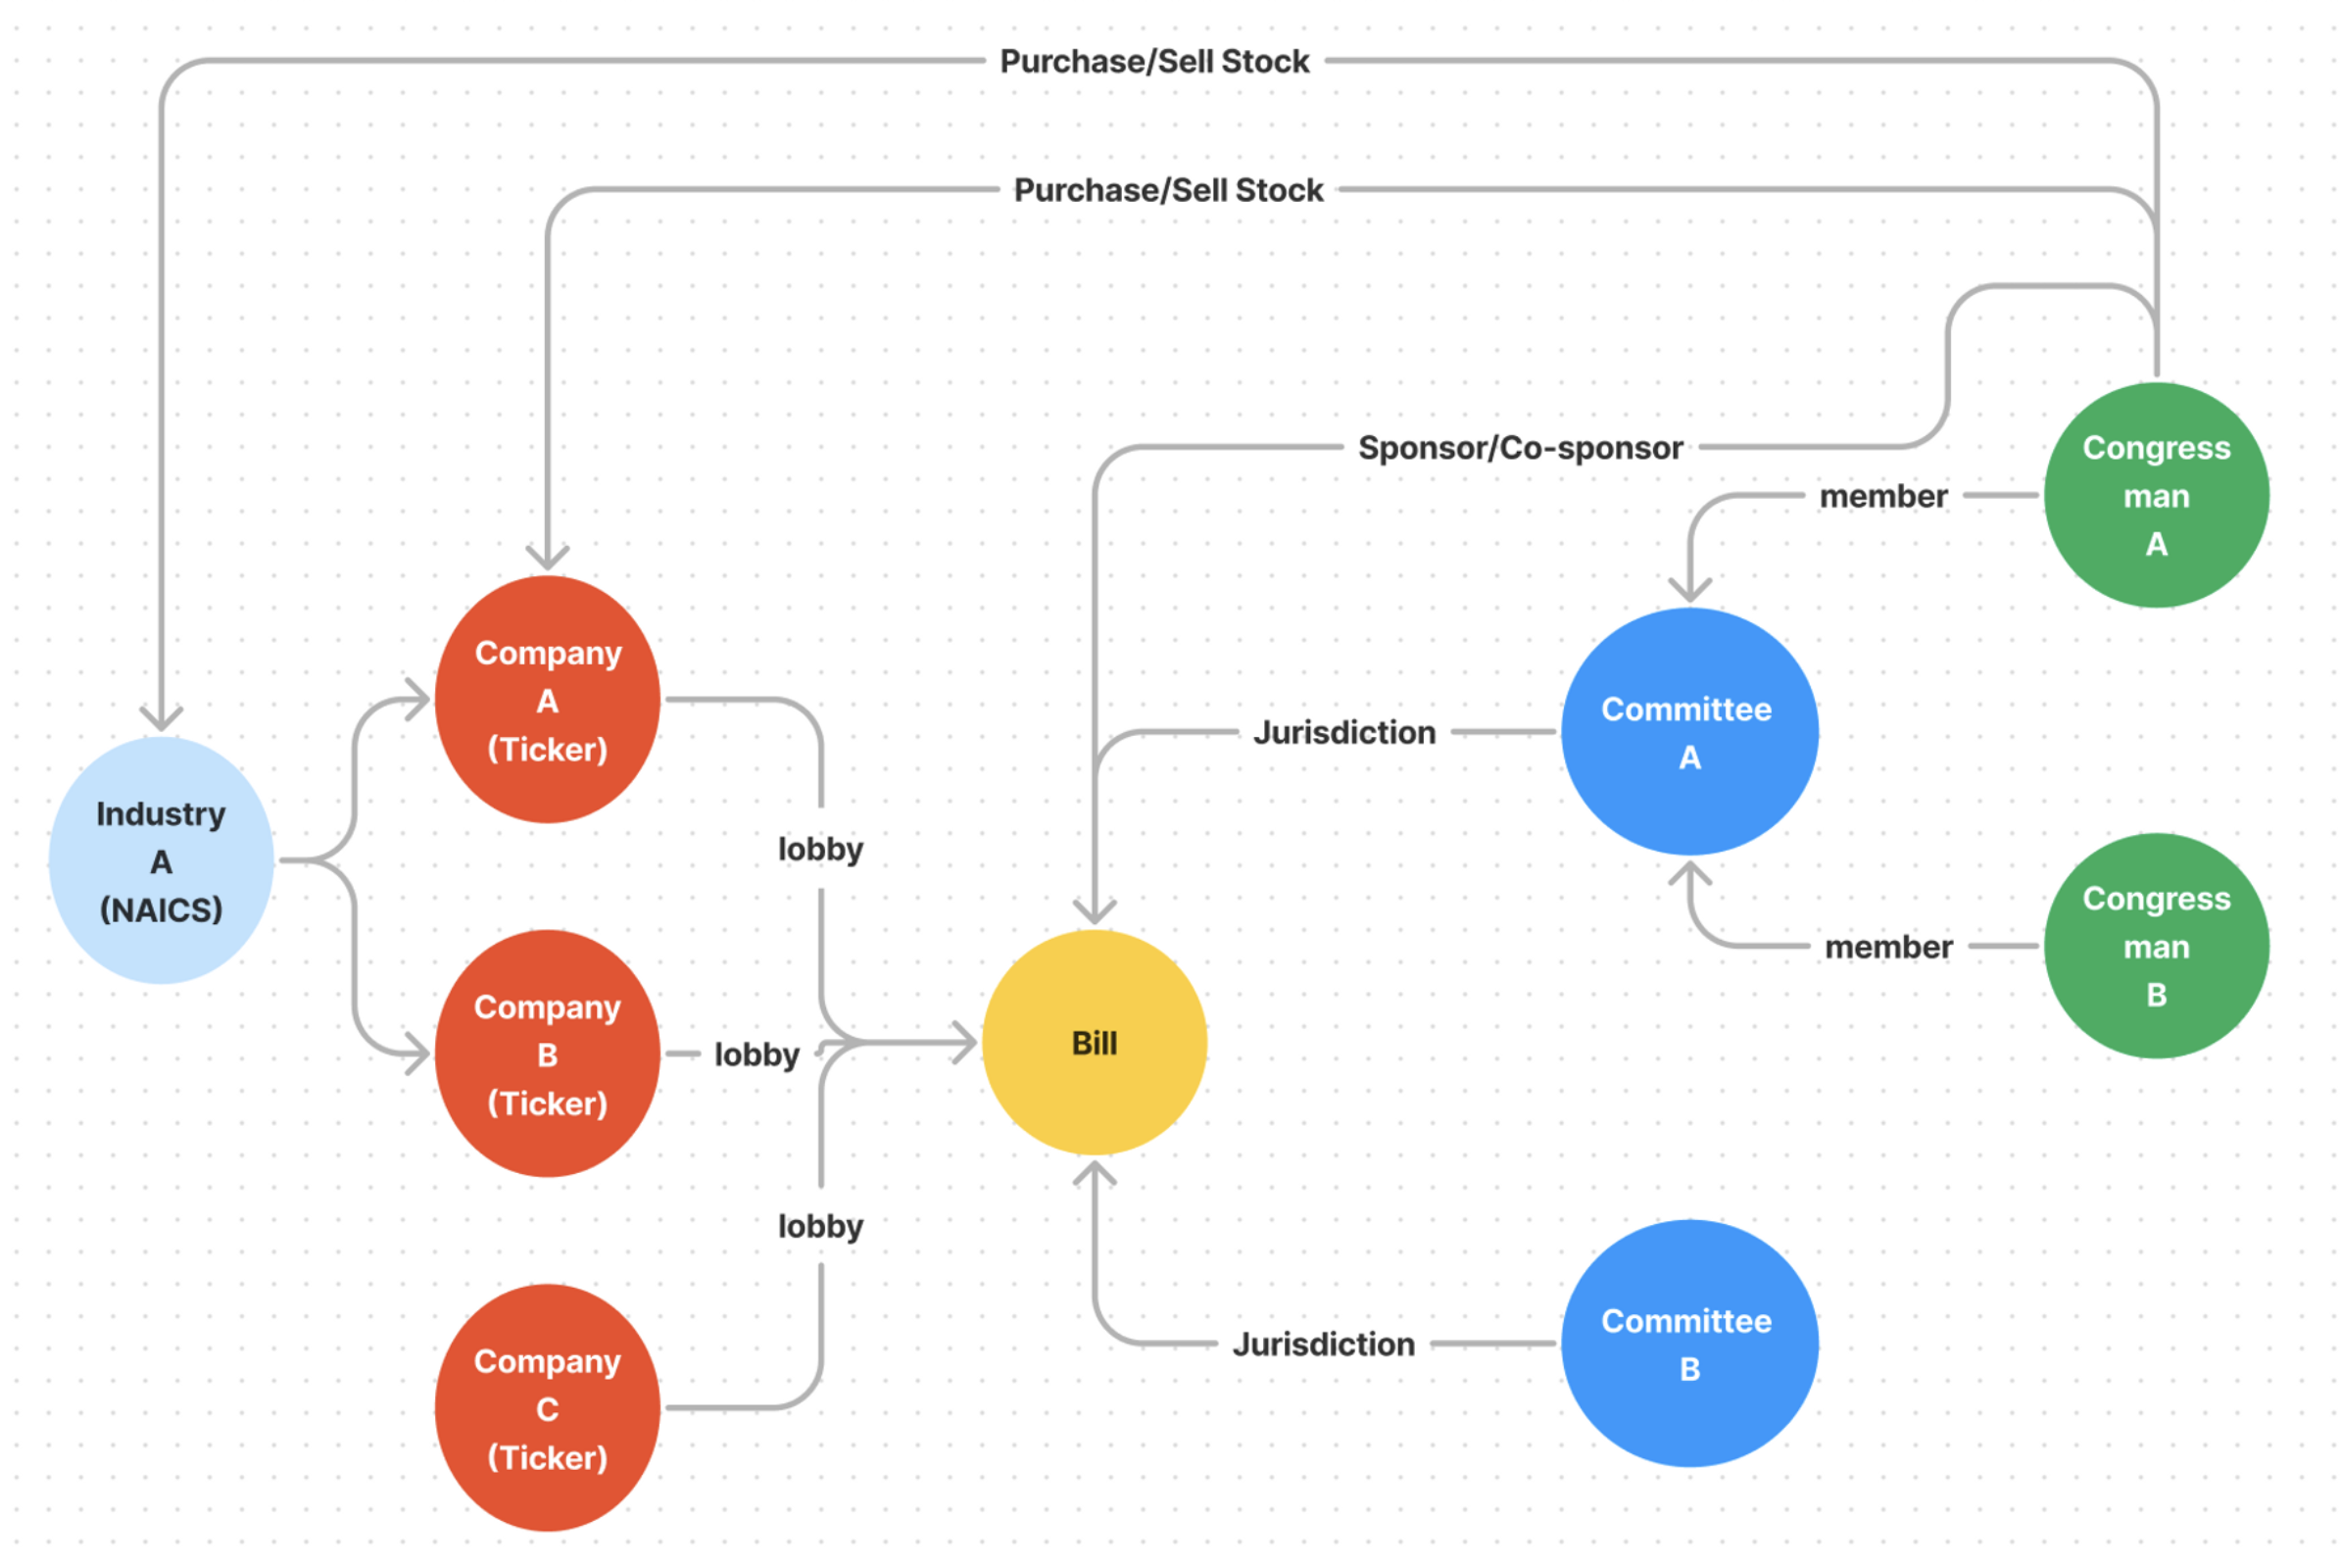
\includegraphics[width=0.75\textwidth]{imgs/graph2.png}
% %   \caption{The graph-structured data captures the congressional knowledge and includes the interactions between different types of entities.}
% %   \label{fig:graph2}
% % \end{figure}

% % \begin{figure}[h]
% %   \centering
% %   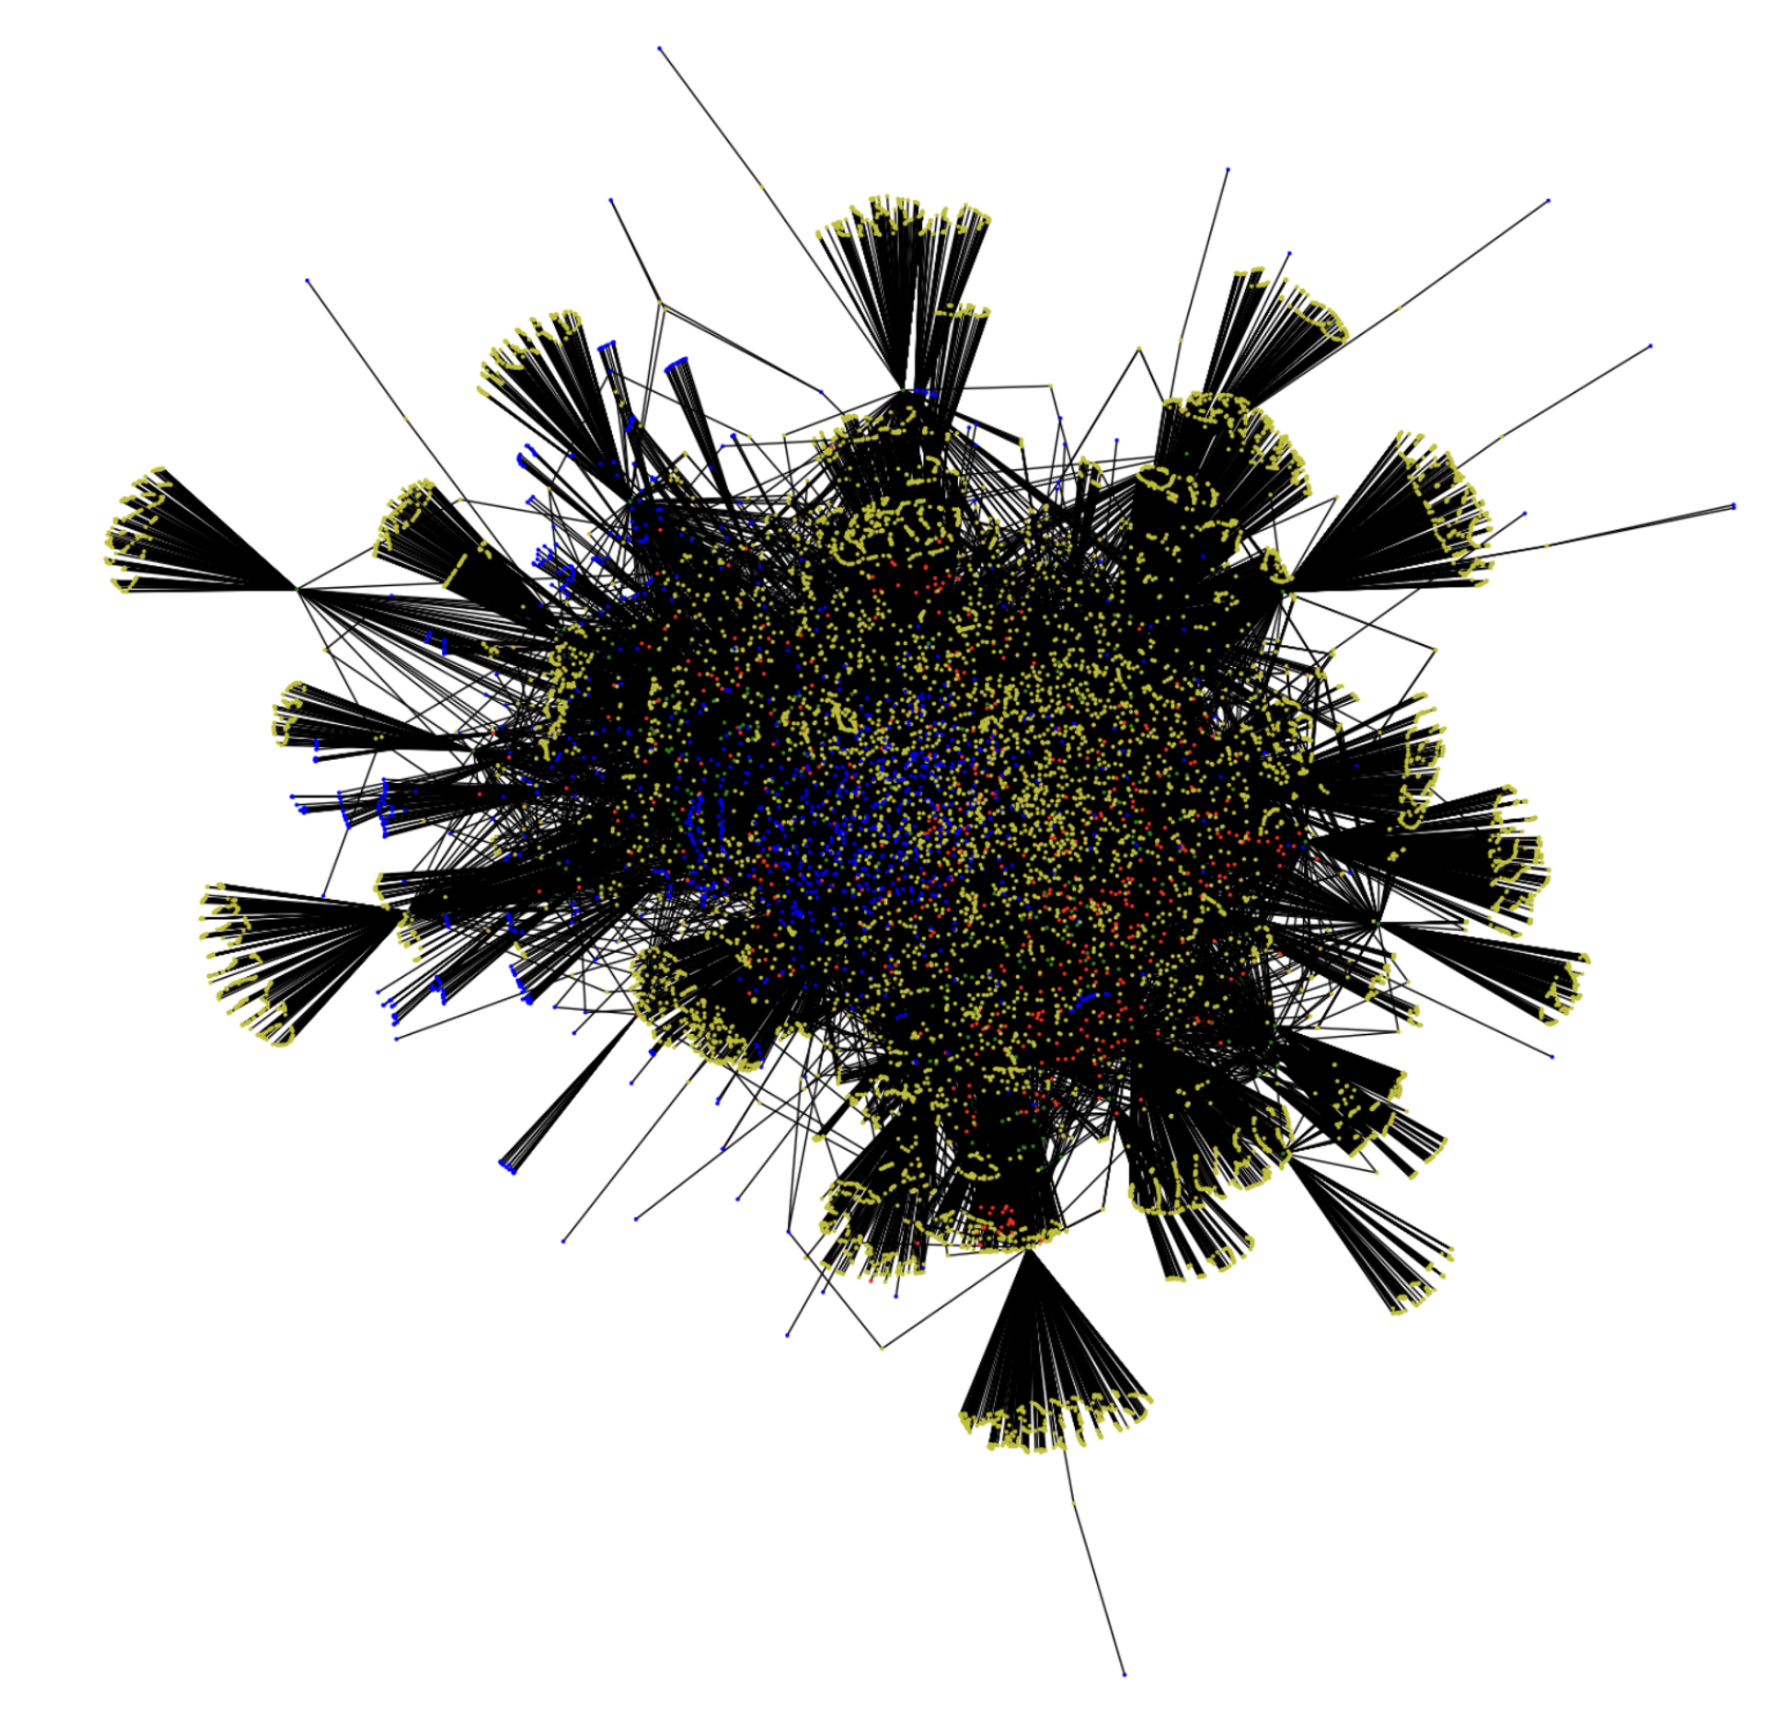
\includegraphics[width=0.75\textwidth]{imgs/graph4.png}
% %   \caption{In the graph-structured data, the yellow, blue, green, and red nodes represent bills, firms, committees, and Congressmen, respectively.}
% %   \label{fig:graph4}
% % \end{figure}


% To examine whether Congress members utilize the knowledge acquired through their positions for personal stock trading, this study estimates the causal effect of committee assignments on their stock transaction patterns. Specifically, the study investigates how being assigned to a particular committee influences the similarity between the NAICS code distribution of a Congress member's portfolio and that of the assigned committee. This is because committee assignments equip Congress members with essential expertise in specific issue areas or industries \citep{Asher1974CommitteesAT}.

% If the transaction patterns of Congress members become more similar to the industry-level information within a committee after being assigned to that committee, it would suggest that they are using their congressional knowledge for personal investment purposes.

% % As an empirical example, Figure \ref{fig:graph5} provides a diagram of Senator Ron Wyden and his NAICS code distribution of personal trading, compared with that of his assigned committee, the Senate Finance Committee (SSFI), and the Senate Banking Committee, of which he is not a member.
% % I calculated the cross-entropy between Ron Wyden's NAICS code distribution of personal trading and that of his assigned committee, the Senate Finance Committee (SSFI), which is 0.717, and that of the Senate Banking Committee (SSBK), of which he is not a member, which is 3.311. A lower cross-entropy value indicates that the two probability distributions are closer in terms of their similarity. Therefore, in Ron Wyden's case, the cross-entropy is a good measurement of the similarity between the committee and the Senator.

% % \begin{figure}[h]
% %   \centering
% %   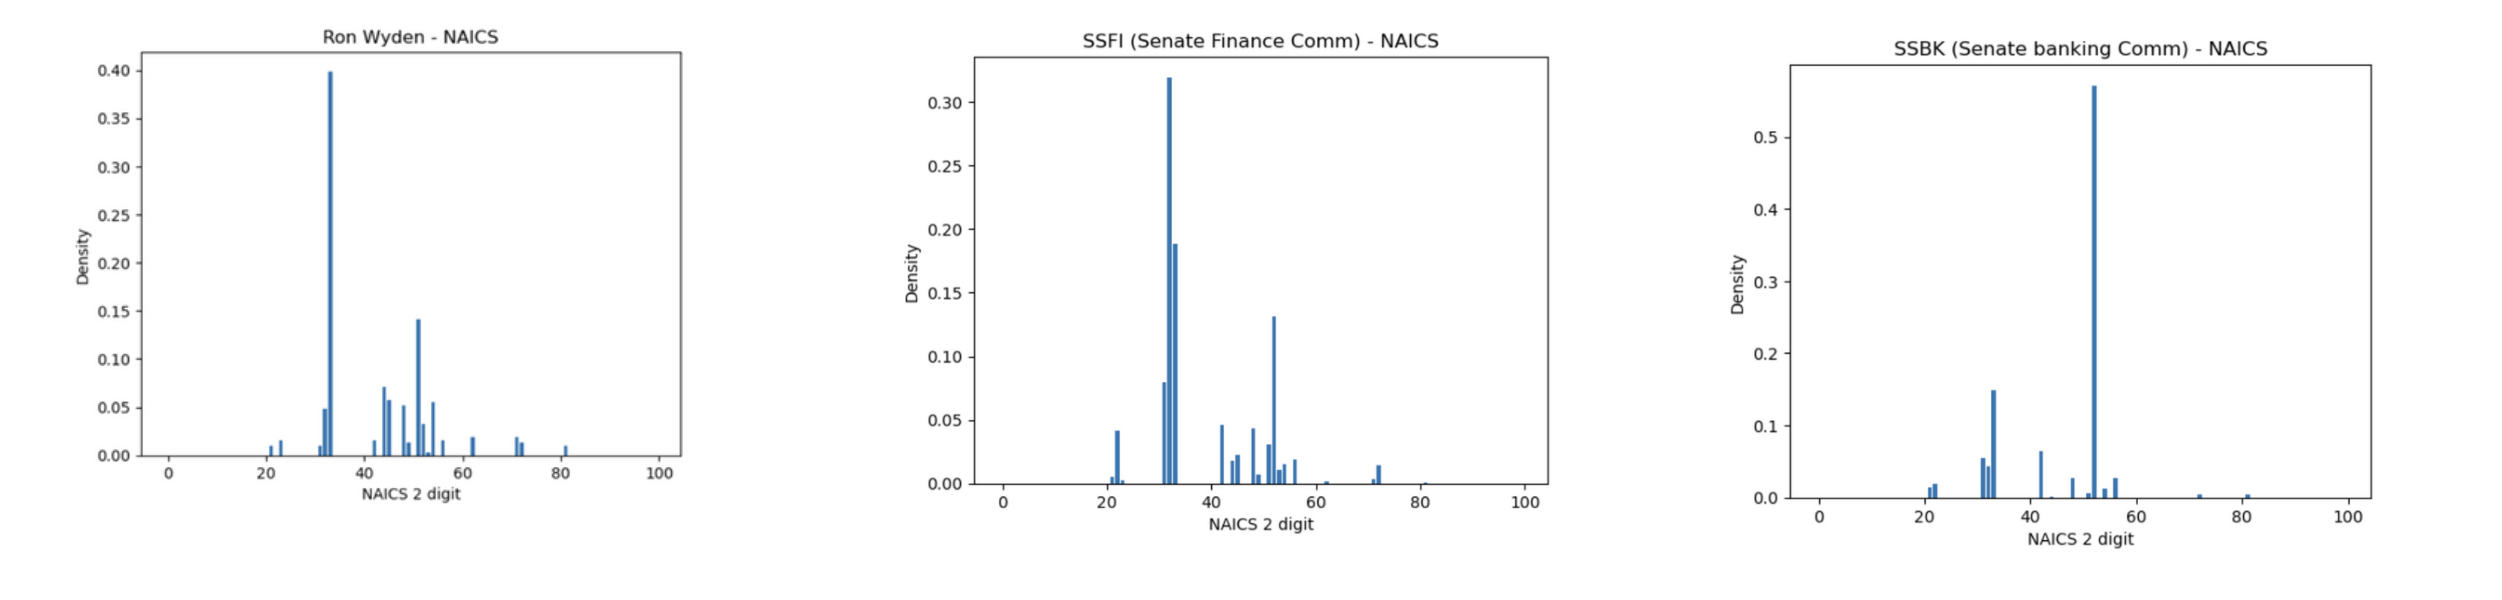
\includegraphics[width=1\textwidth]{imgs/naics.png}
% %   \caption{NAICS code distribution of Senator Ron Wyden's personal trading, compared with that of his assigned committee, the Senate Finance Committee (SSFI), and the Senate Banking Committee, of which he is not a member.}
% %   \label{fig:graph5}
% % \end{figure}


% The primary focus of this study is to estimate the conditional average treatment effect (CATE) of how a Senator's committee assignment affects the similarity between the Senator's and the assigned committee's NAICS code distribution. To estimate this, it is crucial to control for confounding variables that can influence both committee assignment and a Senator's investment behavior. The study assumes that the graph-structured data, which includes information on which firms lobby on which bills, which bills are assigned to which committees, and which Senators are members of which committees, provides all the necessary information to explain a Senator's assignment to a particular committee and their securities transactions. To support this assumption with empirical evidence, the paper will present a preliminary analysis.

% However, unlike widely used tabular data, graph-structured data cannot be directly employed to estimate a quantity of interest through a model. Since the estimation involves mathematical operations over continuous variables, graph data, being a collection of discrete objects, does not have defined operations. Nonetheless, the research emphasizes the importance of using graph-structured data, as it can encompass additional information that explains the relationships between different entities in the network during interactions in congressional activities. To overcome this computational challenge, this paper utilizes Graph Neural Networks (GNN) to learn the appropriate numerical representation specific to each Senator, who resides as a node in the graph. This representation is a numeric vector and is expected to include all the information available from the graph-structured data to explain both a Senator's stock trading behavior and their committee assignment.
% % Finally, by denoting the learned representation of Senator $i$ as $h_i = \phi_{GNN}(i, G)$, the study can estimate the conditional average treatment effect (CATE) by learning estimators for both $\mu_0(h_i) \equiv \mathbb{E}\left[Y_i \mid H=h_i, T_i=0\right]$ and $\mu_1(h_i) \equiv \mathbb{E}\left[Y_i \mid H=h_i, T_i=1\right]$, and using the formula $\text{CATE}(h_i) = \mu_1(h_i) - \mu_0(h_i)$. This allows the study to estimate the effect of committee assignment on the similarity between a Senator's and the assigned committee's NAICS code distribution, while controlling for potential confounders through the learned representation $h_i$.
% % For the estimator of $\mu_0(h_i)$ and $\mu_1(h_i)$, the study will use the Treatment Agnostic Regression Network (TARNet) \citep{tarnet}, which extends T-learners \citep{tlearner} with additional layers of neural networks that learn a shared representation of $h_i = \phi_{GNN}(i, G)$ for the treatment and control groups in a balanced way. By doing so, the neural network can effectively perform its regression task to estimate CATE, even though $h_i$ is asymmetrically distributed between the treatment and control groups.

% There are a total of 62 different committees, and CATE is estimated for each committee separately. By evaluating these CATE values, the paper aims to quantitatively evaluate how committee assignment heterogeneously affects Senators' behavior across committees and among Senators themselves.
% % In addition, it is necessary to control for the confounders to estimate the effect correctly. I assume that the graph-structured data, which includes interactions between firms, bills, committees, and congressmen, and their stock transactions includes all possible confounders that affect committee assignments and their impact on the dependent variable, which is the industry-level similarity between the committee and the congressmen's portfolio. However, in terms of methodology, the question remains about how to control graph-structured data to estimate the treatment effect. Unlike tabular data with numeric values in each item, graph-structured data is a discrete object and thus cannot be computed in typical models.
% % However, thanks to recent developments in representational learning and neural networks, a specific architecture of neural network (called a ``Graph Neural Network'') can learn a good numeric representation of each node by considering its connection with its neighboring nodes in the graph.

% % To determine what constitutes a ``good'' representation of graph-structured data, one can evaluate whether the representation performs the downstream task effectively, which in this case is estimating CATE. The Graph Neural Network learns a representation, denoted as $\phi_{GNN}(X)$, for a given graph-structured data $X$, and I use $\phi_{GNN}(X)$ to estimate the effect of committee assignments on the dependent variable. However, because $\phi_{GNN}(X)$ will be a highly non-interpretable covariate that encodes complex interactions included in the graph, I use meta-learners \citep{metalearner} to estimate CATE using $\phi(X)$. Meta-learners are a family of estimators that combine supervised learning, also known as ``base-learners'', in a specific way while allowing the base learners to take any form, including neural networks. 
% % In this case, I use the Treatment Agnostic Regression Network (TARNet) \citep{tarnet}, which extends T-learners \citep{tlearner}, which is a variant of meta-learners, with additional layers of neural networks that learn a shared representation of $\phi(X)$ for the treatment and control groups in a balanced way. By doing so, the neural network can effectively perform its regression task to estimate CATE, even though $\phi(X)$ is complex, while jointly learning the balanced representation of $\phi(X)$.


% The paper aims to make two main contributions. Firstly, it substantively proves the existence of insider trading by explicitly showing that committee membership changes affect Congressmen's investment behavior to become similar to the information available from the committee. Secondly, it demonstrates a novel methodological approach to estimate causal quantities using graph-structured data by leveraging representation learning via Graph Neural Network. Therefore, the paper proposes a model and learning scheme that combines a Graph Neural Network and meta-learners to learn CATE, conditioning on the output of the Graph Neural Network. 
% % However, the common limitation of these studies is that they do not specify the exact source of congressional knowledge and how that knowledge influences their investment behavior.

% % Although many studies have investigated the investment behavior of congressmen, there are still gaps in the literature. \cite{zi11} and \cite{zi24} found that Senators and House representatives beat the market and enjoy excess returns while \cite{eg13} found that they don't. 
% % However, the common limitation of current work is that they don't specify the exact source of congressional knowledge and how that knowledge affects their behavior.

% % The biggest problem in this line of research is about how to prove they ``do'' invest with which ``privileged knowledge''.
% % The main issue in this area of research is how to prove that politicians are using their inside knowledge to make investments. Just because they make a lot of money from their investments doesn't necessarily mean they are using privileged information. However, many high-profile cases have linked this knowledge to their committee assignments, sponsoring of bills, or their home state and potential connections to local businesses. Therefore, future research should focus on developing a reliable method to track down the sources of this privileged knowledge that is more closely linked to investments that show abnormally high returns. This will help to identify which politicians are involved in unethical financial practices and how they are doing it.


% % In my initial research, I analyzed the excess return for each transaction made by Senators with specific stocks, comparing the return on investment to the federal reserve rates. The results, shown in Figure \ref{fig:agg-ex-r}, suggest that Senators do not generally make significant excess returns from their trading, which is consistent with the findings of \cite{eg13}. However, I did find a few outliers who made substantial gains, some of which have been reported by journalists, while others have not been publicly exposed. An important finding from these outliers is that committee information seems to enable some Senators to enjoy unusually high returns from their trading. 
% % For instance, Senator Ron Wyden from Oregon traded three semiconductor industry stocks, namely AMAT, KLAC, and AVGO, and gained a significant excess return of 170\%, 115\%, and 70\%, respectively (refer to Figure \ref{fig:agg-ex-r}). What stands out is that he bought all three stocks on the same day, April 6, 2020, during a time when the market was falling due to concerns about the pandemic's impact on the economy. He then sold all three stocks on the same day, April 6, 2021, after President Biden proposed a \$50 billion boost to the US chips industry. It is reasonable to assume that Senator Ron Wyden, being the chair of the Senate finance committee, had prior knowledge of this issue before it was made public. This is because the Senate finance committee introduced the bill ``S.3933 - CHIPS for America Act'' after the announcement on June 10, 2020.

% % As another example, Senator Ron Wyden made a 38\% ROI from his investment in an American wine producing company (Constellation Brand, Inc. - Ticker: STZ) when the Trump administration imposed additional tariffs on wines imported from Europe.
% % Since the Senate finance committee has jurisdiction over trade, it is reasonable to assume that Senator Ron Wyden had prior knowledge of this issue before it was made public.

% % In addition, David Perdue, a former senator from Georgia, obtained an estimated excess return of 10\% from his investment in BWX Technologies Inc., a company that supplies nuclear components to the US Navy. What is notable is that he made consecutive purchases of the stock that turned into sales after he was named chairman of the Senate Armed Services Subcommittee on Seapower.

% % \begin{figure}[h]
% %   \centering
% %   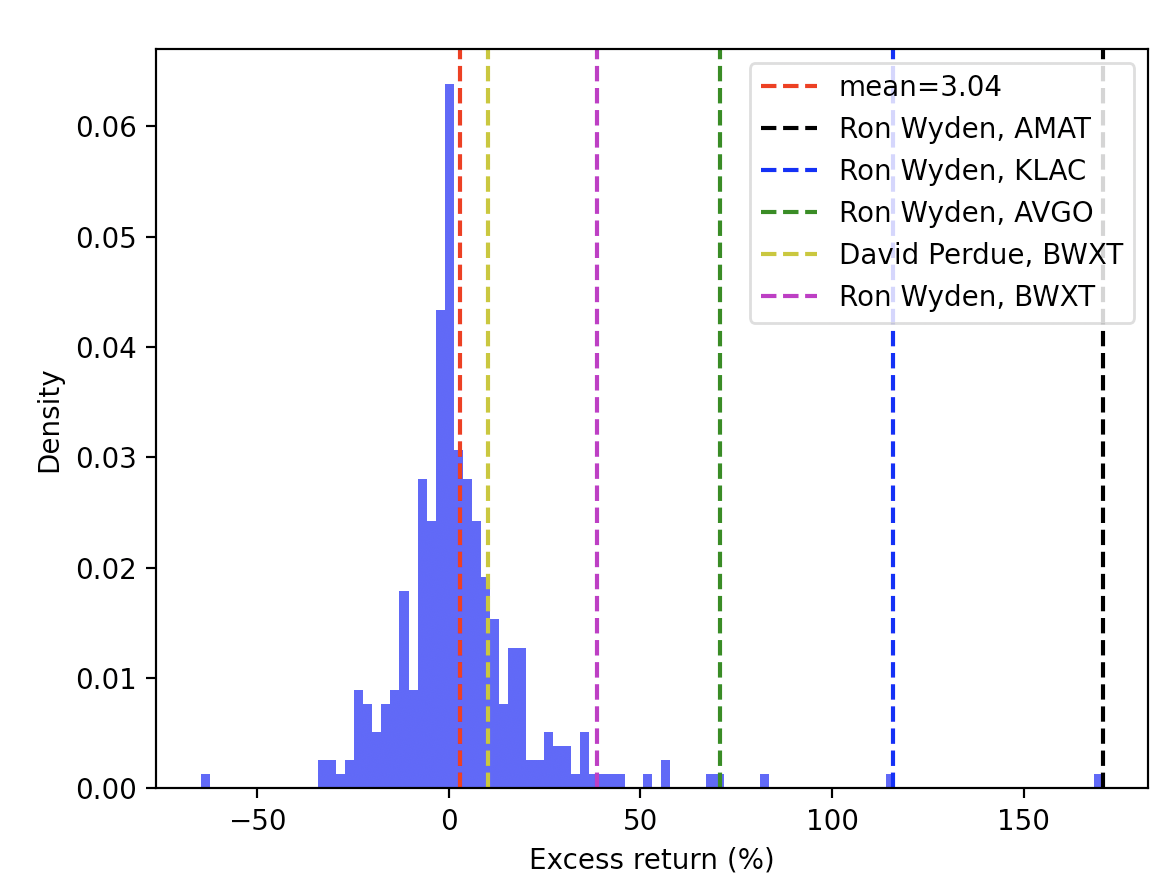
\includegraphics[width=1\textwidth]{imgs/ex-r/aggregate.png}
% %   \caption{Distribution of mean of each distribution of excess return for $333$ distinct pairs of (Senator, Ticker).}
% %   \label{fig:agg-ex-r}
% % \end{figure}

% % \begin{figure}[h]
% %   \centering
% %   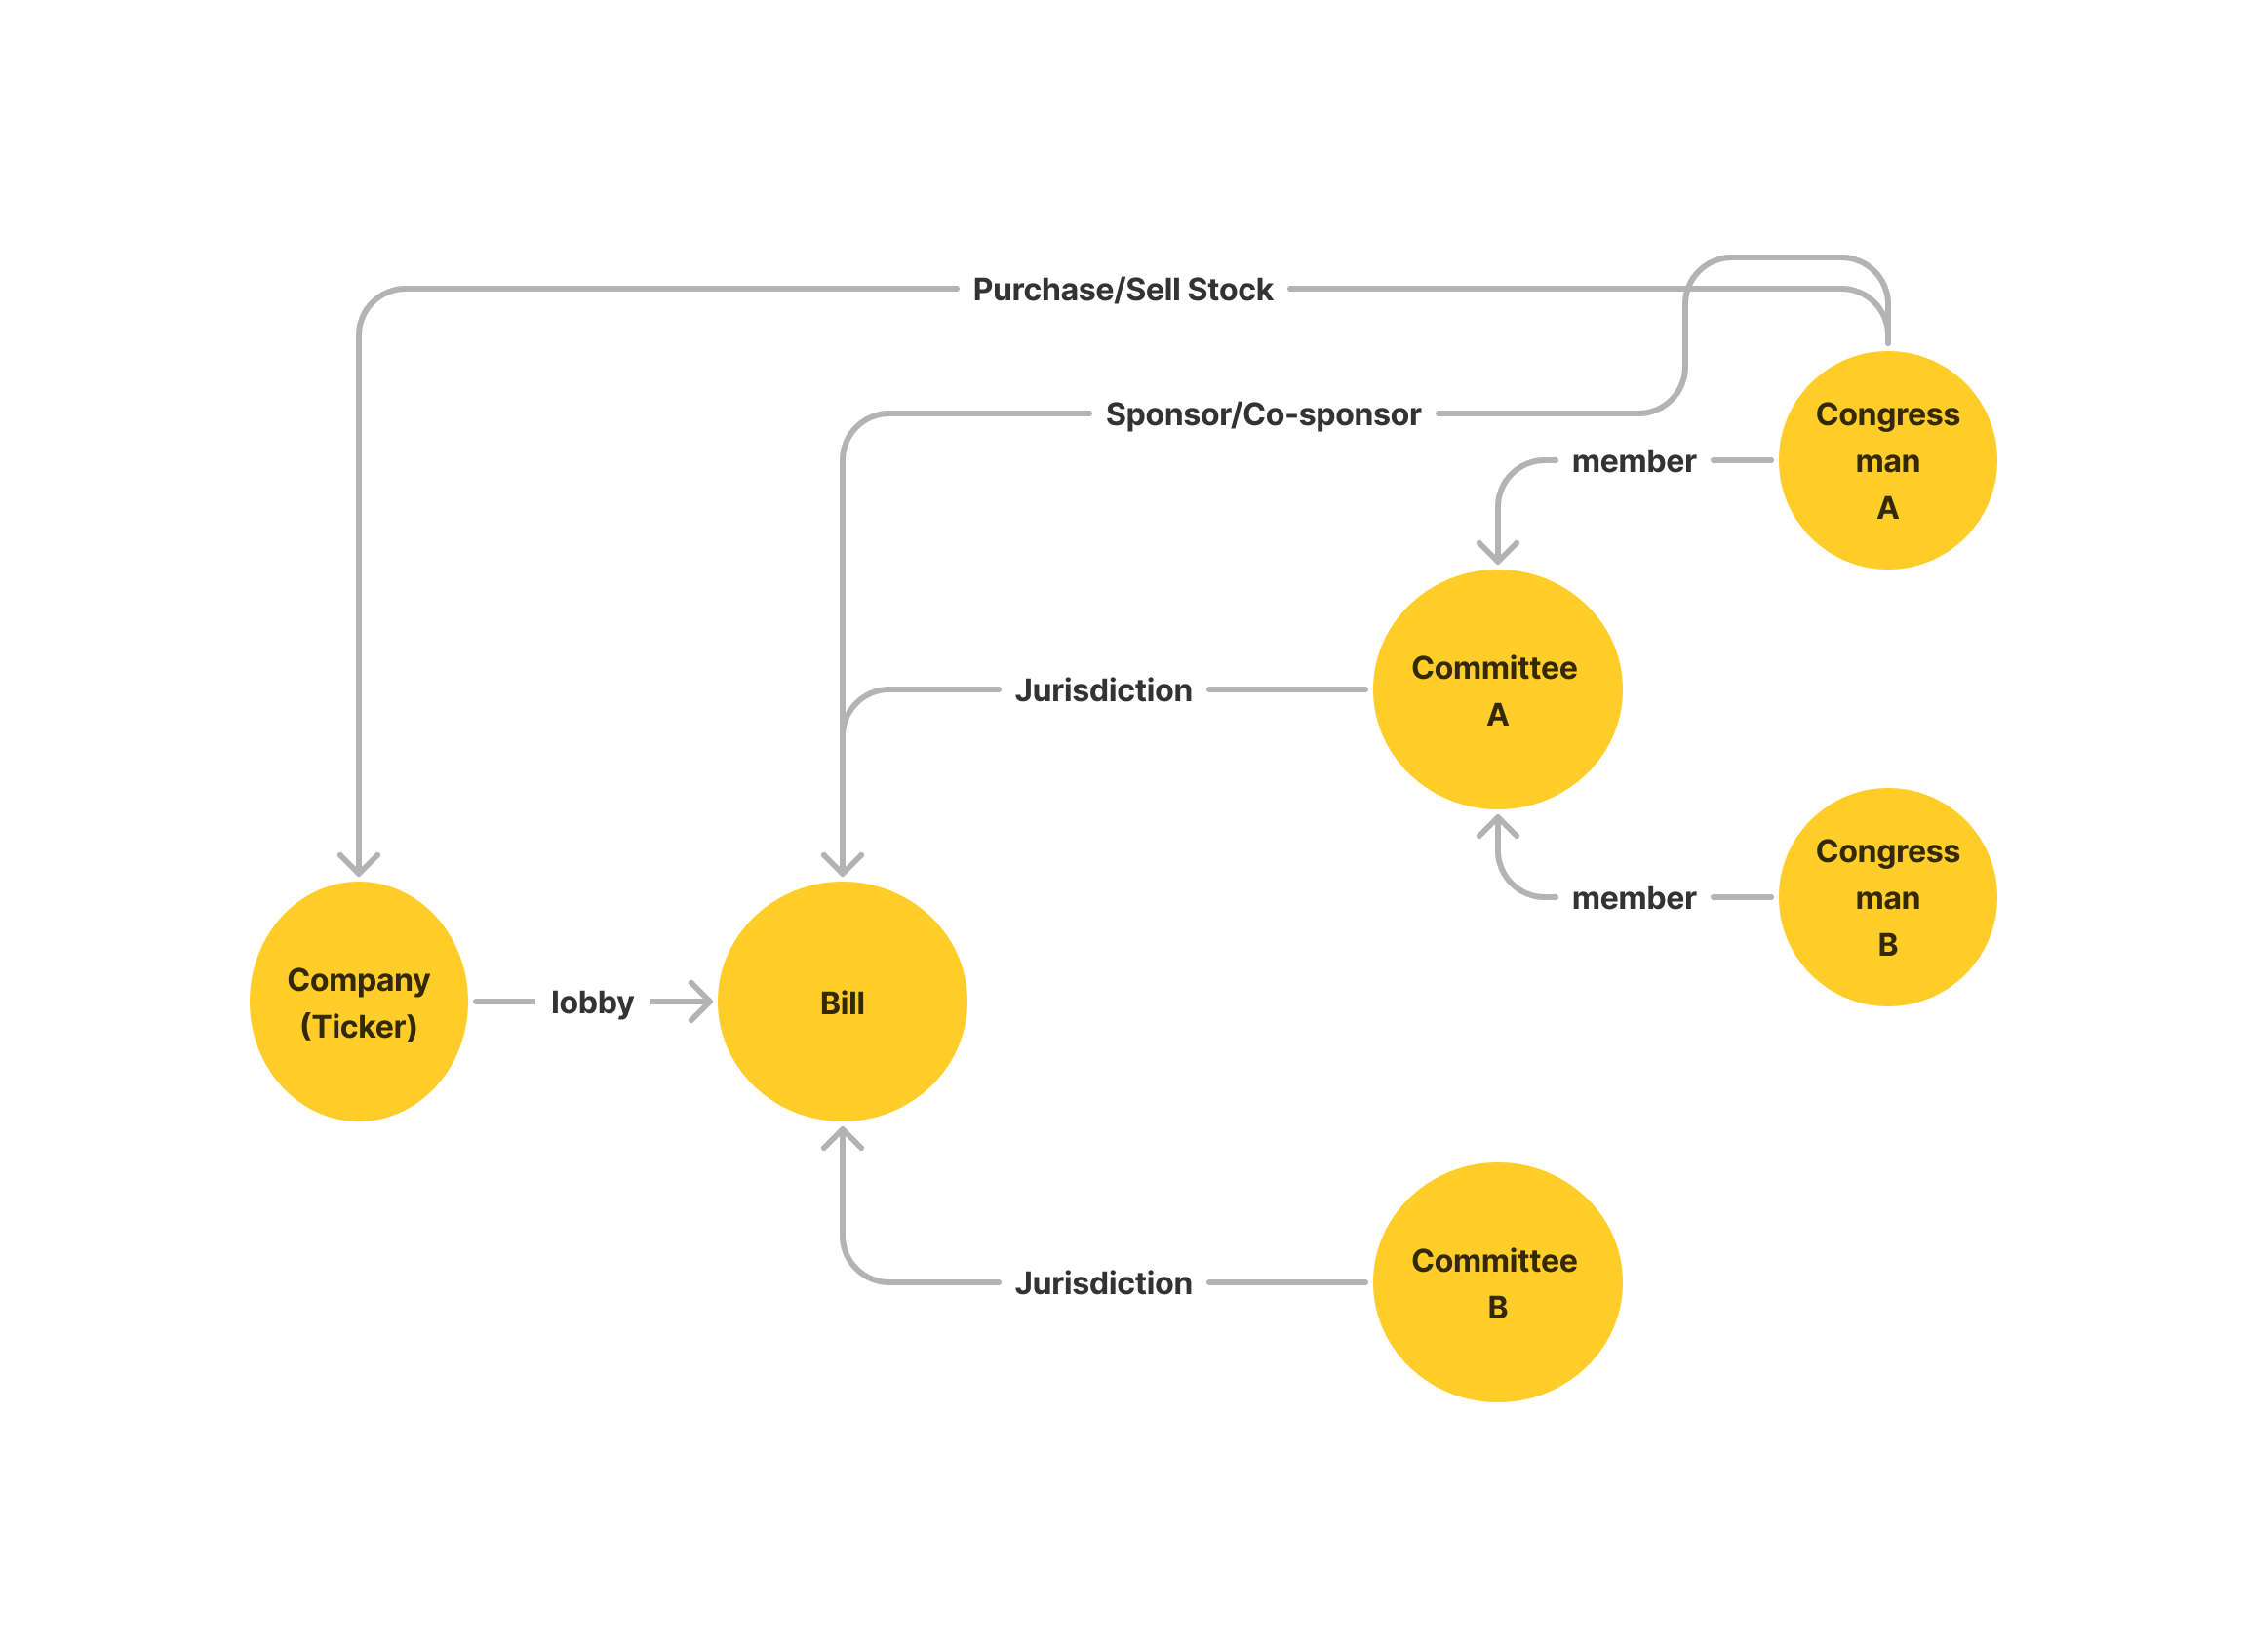
\includegraphics[width=1\textwidth]{imgs/cgd.png}
% %   \caption{Interaction graph between committees, bills, companies, and congressmen in congressional investment.}
% %   \label{fig:cbd}
% % \end{figure}


\section{Estimating Excess Returns of Congressional Stock Trading} \label{ex-r}

\footnote{Reproducible code for this section is available at \url{https://github.com/syyunn/efd/blob/main/anlys/cashout/fifo-rd-fed-pppsss-include-etf.py}}The broader literature on insider trading has long explored the information advantages that certain individuals, such as corporate insiders or well-connected investors, may possess when trading in the stock market. For example, \cite{jeng2003} estimated returns to insider trading from a performance-evaluation perspective, while \cite{ivkovic2005} studied the information content of the geography of individual investors' common stock investments. These studies highlight the importance of understanding the impact of information asymmetry and potential insider trading in financial markets.

Despite the extensive research on insider trading in general, the application of this approach to congressional stock trading has been limited. In the context of congressional stock trading, previous studies, such as those conducted by \cite{zi24}, \cite{zi11} and \cite{eg13}, have predominantly used calendar-time based portfolio approaches \citep{hdz07} to estimate excess returns. This involves creating synthetic buy and sell portfolios \citep{syn1,syn2} that mimic congresspersons' stock purchases and sales but sell or buy such stocks after a year. 
  This approach, however, neglects the importance of transaction timing, which is a crucial aspect of insider trading \citep{tahoun2014,schweizer2011}. It does not account for the short-term fluctuations in stock prices that congresspersons might anticipate based on their access to privileged information. Congresspersons could potentially profit from these expected fluctuations by strategically timing their transactions using their privileged knowledge.  This presents a severe limitation in understanding the true extent of potential insider trading among U.S. members of Congress.

In addition, averaging excess returns across congresspersons may not capture the full extent of insider trading within the inner circle of Washington D.C. politics. \cite{schweizer2011} provided anecdotal evidence of politicians and their friends profiting from insider stock tips, 
while \cite{lim2009} studied corruption and wealth accumulation in Congress, and \cite{jerke2010} and \cite{bainbridge2010}
examined the use of political intelligence for insider trading with several anecdotes. 
These case studies suggest that certain congresspersons might engage in insider trading with specific firms or industries,
 which would be overlooked in an aggregate analysis.

In this section, therefore, I aim to address these limitations by estimating the excess returns at the congressperson-ticker level, with a focus on the life cycle of each buy/sell chain of specific tickers consecutively transacted by a congressperson. This approach offers a more granular analysis of potential insider trading among U.S. members of Congress, allowing us to better evaluate whether widespread insider trading exists at the congressperson-ticker level. By doing so, we build upon both the general insider trading literature and the existing research on congressional stock trading, contributing to a more comprehensive understanding of the potential information advantages leveraged by politicians in the stock market and the importance of transaction timing.

\subsection{Data}\label{sen-data}

To estimate excess returns at the congressperson-ticker level, I first needed to compile comprehensive data on the stock transactions of U.S. members of Congress. I obtained this data by scraping the Senate Financial Disclosure website\footnote{\url{https://efdsearch.senate.gov/search/home/}}, which provides detailed information about the stock transactions made by congresspersons, including the date, ticker symbol, and the amount of each transaction.

The resulting dataset consists of 25,023 transactions, spanning a period from January 1, 2014, to August 5, 2022. These transactions involve 74 distinct Senators and 2,114 distinct tickers. Among these tickers, around 40\% (832) are individual company-level tickers, such as AAPL for Apple Inc. and AMAT for Applied Materials Inc., while the remaining 60\% (1,282) are ETFs or mutual funds, like QQQ for Nasdaq-100 index funds or IHI for U.S. Medical Devices ETF.
This prevalence of industry-level security transactions suggests that Congresspersons often trade based on broader industry trends, rather than focusing solely on specific firms. This observation urges a recalibration of current literature \citep{zi11,zi24, eg13, eg14}, which tends to focus predominantly on firm-level stock trading behavior. Instead, it highlights the necessity of broadening our perspective, embracing a more comprehensive unit of analysis that extends beyond the firm-level, to include industry or theme-level stock trades.

For each transaction, I added the Volume Weighted Average Price (VWAP) in USD acquired from a commercial stock data API \footnote{\url{https://polygon.io/stocks}}. VWAP is a widely used trading benchmark \citep{vwap1, vwap2, vwap3} that represents the average price at which a security is traded throughout the day, weighted by the volume of each trade. By using VWAP, I obtained a representative price for each stock transaction, taking into account the varying trading volumes and prices during the entire trading day.
However, the Senate Financial Disclosure data is range-censored in terms of the ``amount'', which represents the value of the stock transaction for that date. The amount is reported as one of the following ranges in Table \ref{tb:rg}.

\begin{table}[h]
  \centering
  \begin{tabular}{c}
  \hline
  Amount Range (USD) \\
  \hline
  1,001 - 15,000 \\
  15,001 - 50,000 \\
  50,001 - 100,000 \\
  100,001 - 250,000 \\
  250,001 - 500,000 \\
  500,001 - 1,000,000 \\
  1,000,001 - 5,000,000 \\
  5,000,001 - 25,000,000 \\
  \hline
  \end{tabular}
  \caption{Range of the min-max amount of each stock transaction.}
  \label{tb:rg}
\end{table}



\begin{figure}[h]
  \centering
  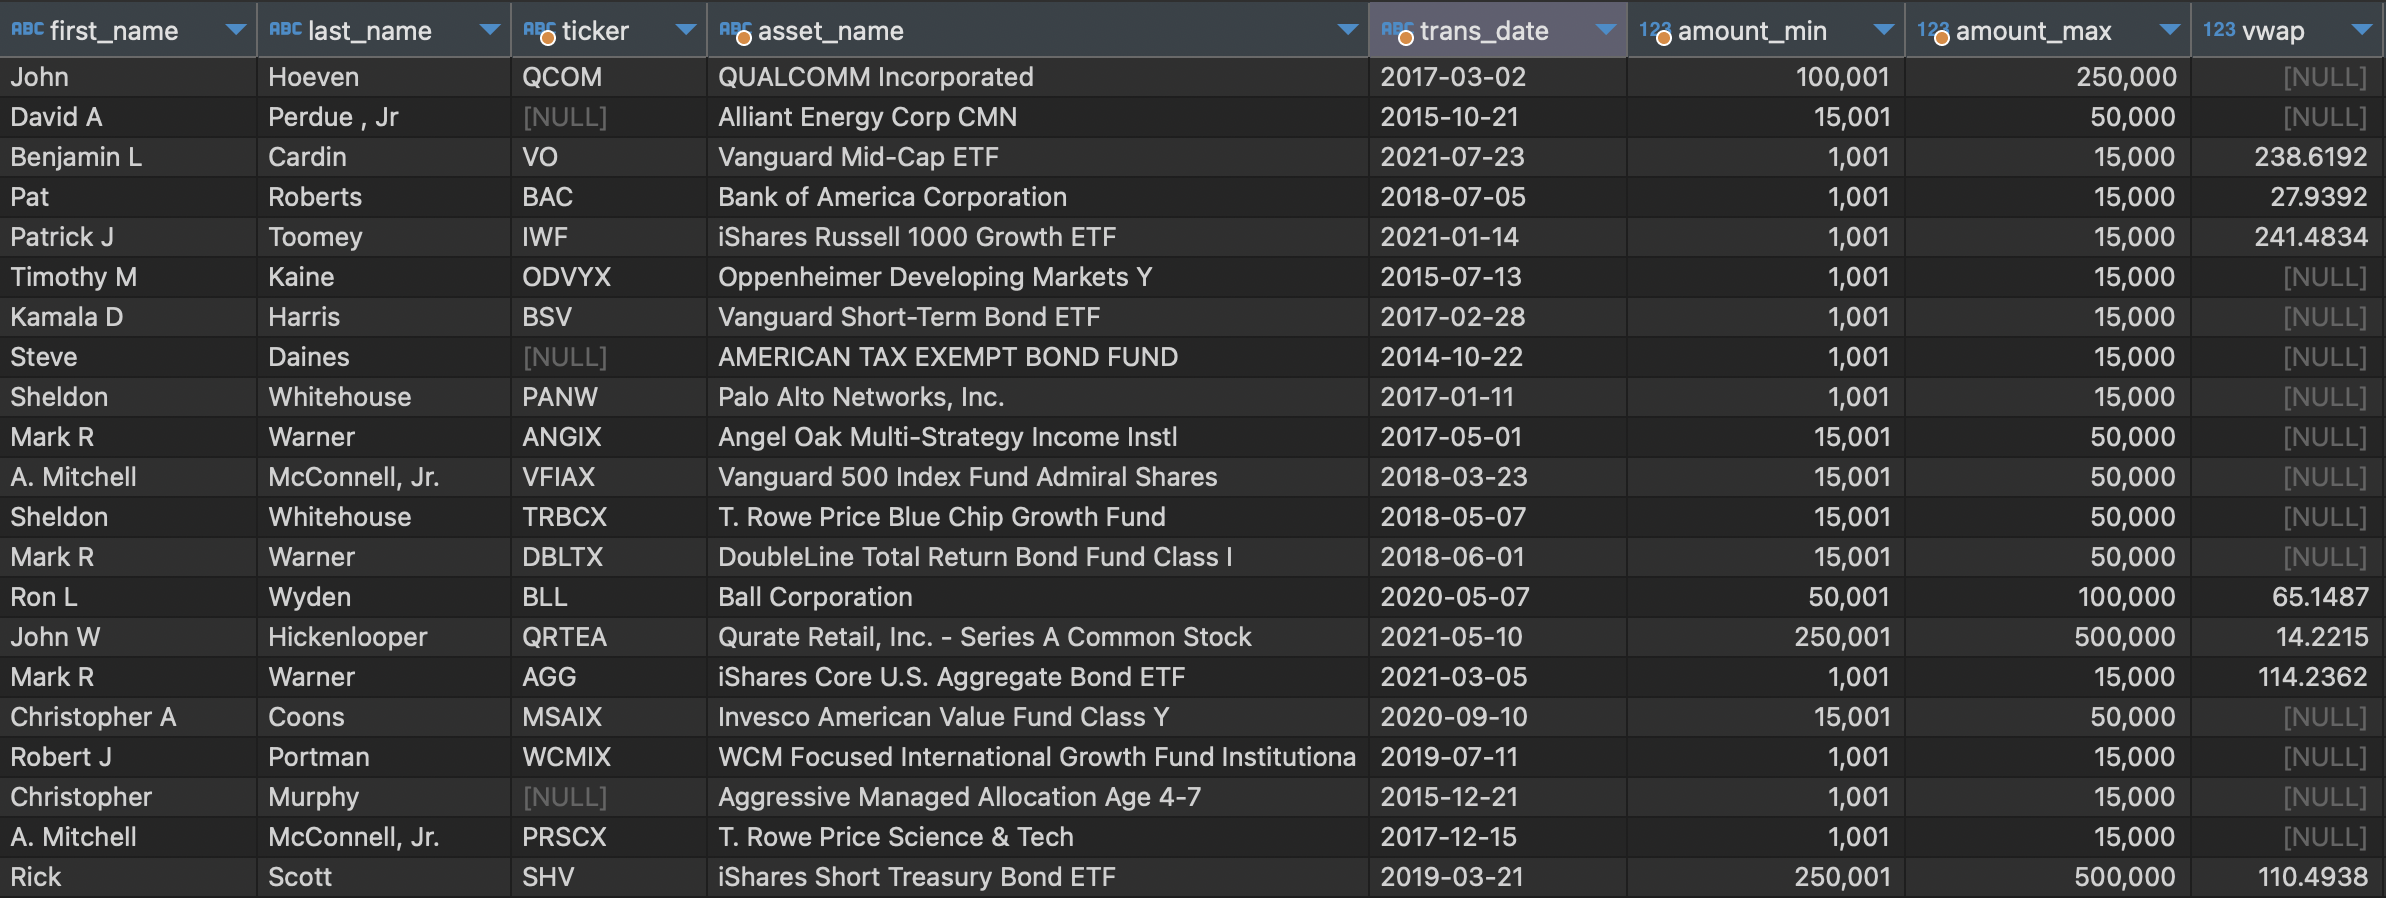
\includegraphics[width=1\textwidth]{imgs/tb-trans.png}
  \caption{\textbf{Senator's Stock Transactions Data (Compiled)} The table shows the compiled stock transactions data which includes the name, ticker, date, amount min/max, and VWAP for each transaction.}
  \label{fig:trans-example}
\end{figure}

It is important to note that not all of the transactions have a clear ticker because some assets are not publicly traded on an exchange (See ``NULL'' values in ticker field in Figure \ref{fig:trans-example}). Additionally, not all transactions have VWAP values, as not all tickers or asset names have available stock price data from the data provider (See ``NULL'' values in vwap column in Figure \ref{fig:trans-example}). This may lead to some limitations in the analysis, but the dataset still provides a rich source of information for understanding potential insider trading among U.S. members of Congress. An excerpt of a few rows of such compiled transaction data is provided in Figure \ref{fig:trans-example}.

\subsection{Uncanny Timing of Congressional Stock Trading} \label{uct}

Firstly, I gained insights into the mechanisms behind their trading decisions by reviewing news articles. For example, there were several media reports\footnote{Theo Wayt, ``US Sen. Ron Wyden boosts chipmakers while his wife buys their shares'', New York Post, May 20, 2021, \url{https://nypost.com/2021/05/20/us-sen-ron-wyden-boosts-chipmakers-while-his-wife-buys-their-shares/}}\footnote{ Alicia Parlapiano, Adam Playford, and Kate Kelly, ``These 97 Members of Congress Reported Trades in Companies Influenced by Their Committees'', The New York Times, Sept. 13, 2022, \url{https://www.nytimes.com/interactive/2022/09/13/us/politics/congress-members-stock-trading-list.html}}
regarding Ron Wyden's semiconductor stocks trading.
I searched for Senator Ron Wyden's stock transactions with a NAICS code beginning with 334, which indicates computer and electronic product manufacturing.
I found that three different tickers (AMAT, AVGO, KLAC) of the transactions that met this condition have a commonality in that they all started on the same date, April 6th, 2020, and ended on either April 6th or April 16th, 2021. Furthermore, all of them follow a similar pattern of multiple purchases followed by sales after certain critical points, such as $Purchase-Purchase- \hdots - Purchase \text{ } |  \text { } Sales - Sales - \hdots - Sales$ as shown in Fig \ref{fig:trans}.

\begin{figure}[h]
  \centering
  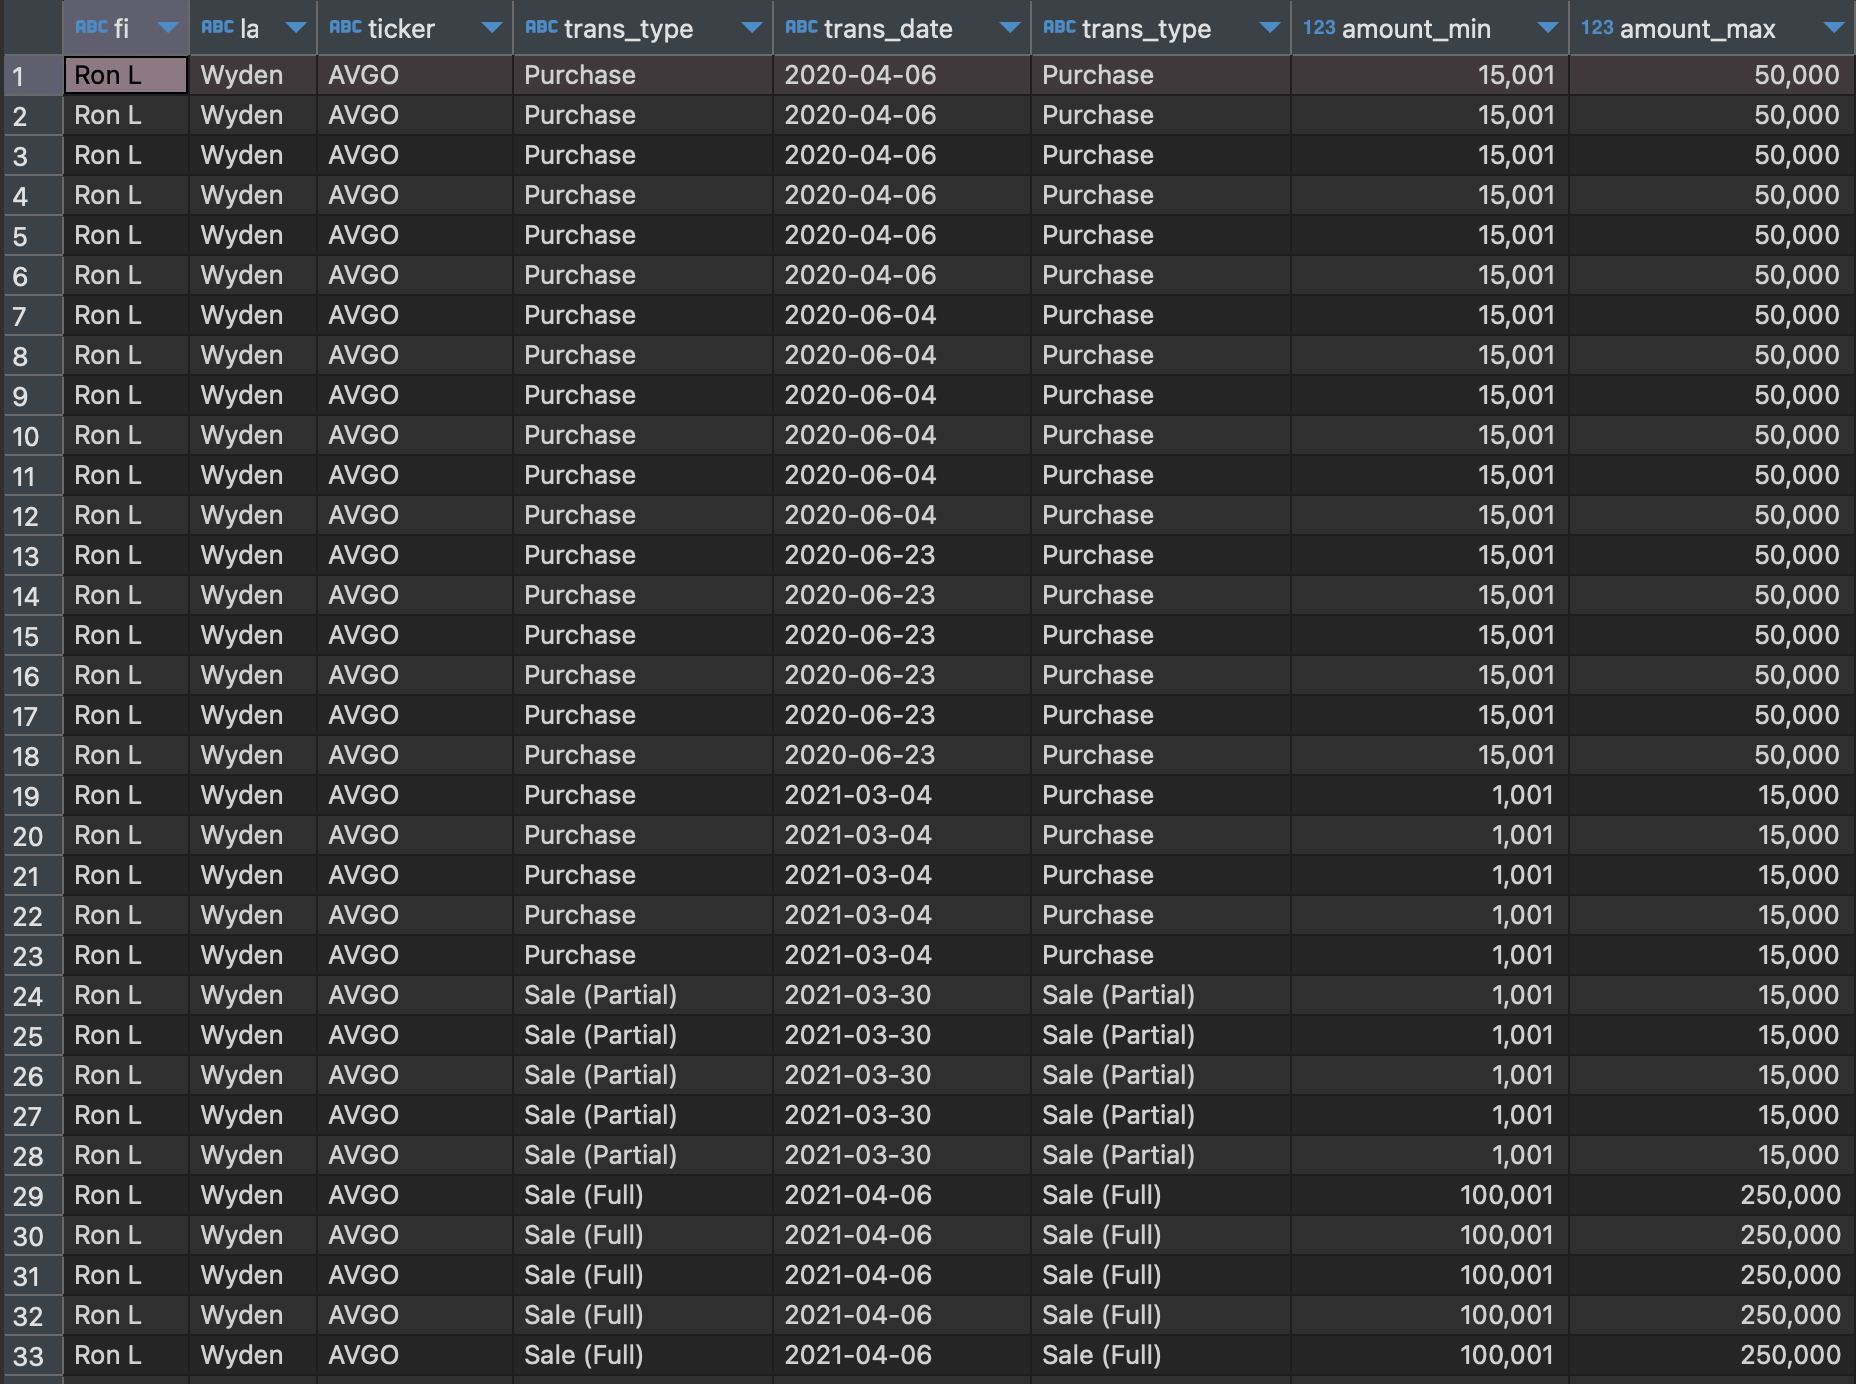
\includegraphics[width=1\textwidth]{imgs/trans.png}
  \caption{\textbf{Senator Ron Wyden's stock transactions for Broadcom Inc. (Ticker: AVGO)} The transactions exhibits a pattern of multiple purchases followed by sales after certain critical points, spanning from April 6th, 2020 to April 6th, 2021.}
  \label{fig:trans}
\end{figure}

On April 1st, 2021, President Biden announced a plan to invest \$50 billion to boost the U.S. chip industry\footnote{Alex Leary and Paul Ziobro, ``Biden Calls for \$50 Billion to Boost U.S. Chip Industry'', The Wall Street Journal, March 31, 2021, \url{https://www.wsj.com/articles/biden-urges-50-billion-to-boost-chip-manufacturing-in-u-s-11617211570}}. After this announcement, Senator Ron Wyden sold all of his semiconductor stocks. This suggests that members of Congress may have access to not only legislative information but also the publicization of such information that can potentially move the stock market beforehand. This enables them to not just design their portfolio, but also determine when to buy and when to sell, with some anticipation of specific events and their impact on the market.

As shown in the example of Ron Wyden, importance of timing in the context of political insider trading is emphasized by scholars like \cite{tahoun2014} and \cite{schweizer2011}. 
Accordingly, this research proposes to integrate such timing considerations into the analysis of excess returns. Specifically, we will adopt an approach that recognizes the life-cycle of transactions, starting from consecutive purchases and ending with consecutive sales. This methodology will be detailed further in Section \ref{subsq}, ensuring that our analysis is cognizant of both the decision to invest in specific stocks and the timing of these decisions.






\subsection{``Purchsaes-then-Sales'': Sub-sequences of Congressional Stock Transactions} \label{subsq}

Based on the observation introduced in Section \ref{uct}, I partitioned each transaction sequence into sub-sequences, where each sub-sequence consists of consecutive purchase transactions followed by consecutive sale transactions, all arranged in chronological order as illustratively shown in Figure \ref{fig:transaction_partition}. 
This kind of sub-sequence partitioning is based on the assumption that if congressional investments involve insider trading—using privileged knowledge—there should be a timing of both the beginning and end of the investment that is driven by a certain event \citep{event1, event2}. Specifically, the event of interest would be one that, upon being publicized, moves the stock market into a different phase. In the case of insider trading, we would expect to see a pattern where a congressperson accumulates a long position in a stock ahead of a positive event and subsequently monetizes that position by selling the stock after the event becomes public and positively impacts the stock price. Conversely, a congressperson may sell a stock ahead of a negative event and avoid losses when the event becomes public and negatively impacts the stock price.

It is important to note that in this analysis, we are only considering the case of congresspersons taking long positions and subsequently selling those positions, as this is the type of transaction that is reported in Financial Disclosure reports. In these reports, there are no ``stock-shorting'' transactions, which involve betting against a stock and profiting from its decline. As such, our partitioning approach focuses on identifying sub-sequences of consecutive purchases followed by consecutive sales, which may reflect the use of privileged knowledge to take advantage of market-moving events and realize profits from long positions.

\begin{figure}[ht]
  \centering
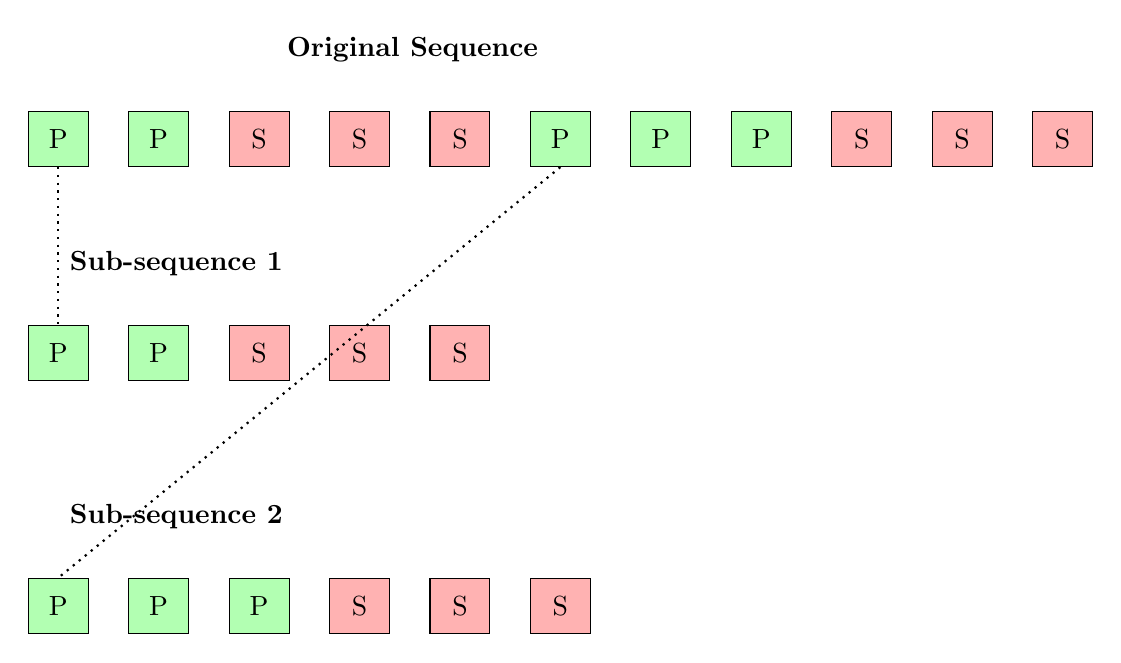
\begin{tikzpicture}[node distance=0.5cm, auto]
  \tikzstyle{purchase} = [rectangle, draw, fill=green!30, text width=1.5em, text centered, minimum height=2em]
  \tikzstyle{sale} = [rectangle, draw, fill=red!30, text width=1.5em, text centered, minimum height=2em]

  % Original sequence
  \node [purchase] (p1) {P};
  \node [purchase, right=of p1] (p2) {P};
  \node [sale, right=of p2] (s1) {S};
  \node [sale, right=of s1] (s2) {S};
  \node [sale, right=of s2] (s3) {S};
  \node [purchase, right=of s3] (p3) {P};
  \node [purchase, right=of p3] (p4) {P};
  \node [purchase, right=of p4] (p5) {P};
  \node [sale, right=of p5] (s4) {S};
  \node [sale, right=of s4] (s5) {S};
  \node [sale, right=of s5] (s6) {S};

  % Sub-sequence 1
  \node [purchase, below=of p1, yshift=-1.5cm] (sp1) {P};
  \node [purchase, right=of sp1] (sp2) {P};
  \node [sale, right=of sp2] (ss1) {S};
  \node [sale, right=of ss1] (ss2) {S};
  \node [sale, right=of ss2] (ss3) {S};

  % Sub-sequence 2
  \node [purchase, below=of sp1, yshift=-2cm] (sp3) {P};
  \node [purchase, right=of sp3] (sp4) {P};
  \node [purchase, right=of sp4] (sp5) {P};
  \node [sale, right=of sp5] (ss4) {S};
  \node [sale, right=of ss4] (ss5) {S};
  \node [sale, right=of ss5] (ss6) {S};

  % Labels
  \node [above=of p1, xshift=4.5cm, font=\bfseries] (origLabel) {Original Sequence};
  \node [above=of sp1, xshift=1.5cm, font=\bfseries] (sub1Label) {Sub-sequence 1};
  \node [above=of sp3, xshift=1.5cm, font=\bfseries] (sub2Label) {Sub-sequence 2};

  % Dotted line
  \draw [dotted, thick] (p1.south) -- (sp1.north);
  \draw [dotted, thick] (p3.south) -- (sp3.north);

% % Arrows
% \draw [->, thick] (origLabel.south) -- ++(0, -0.5cm) -| (sub1Label.north);
% \draw [->, thick] (origLabel.south) -- ++(0, -0.5cm) -| (sub2Label.north);
\end{tikzpicture}
\caption{Partitioning of transaction sequences into sub-sequences based on consecutive purchase and sale transactions.}
\label{fig:transaction_partition}
\end{figure}
% Based on this observation, I developed an algorithm to calculate the excess returns for each (Senator, Ticker) pair. Unlike previous literature \citep{zi11, zi24, eg13} that computes excess returns at the year-chamber level, such as the excess return of the Senate or House over a specific year, I hypothesized that insider trading occurs in a time-specific manner. Therefore, it should be estimated accordingly, rather than a year-based approach. As a result, I selected all transaction chains that start with multiple purchases followed by sales within six months of the transition from purchase to sale.

Through the partitioning process, I obtained a total of 435 sub-sequences spanning across 358 unique combinations of Senator-Ticker pairs.
Each sub-sequence represents a long position taken by a senator in a specific stock and is characterized by a start date and an end date.
The start date corresponds to the date of the first purchase transaction in the sub-sequence, and the end date corresponds to the date of the last sale transaction in the sub-sequence. The duration of each sub-sequence, measured in days, represents the length of time the senator held the long position. 
On average, senators held such long positions for approximately 340 days, and around 65\% of these positions were held for less than a year. The frequencies of durations for all subchains are illustrated in Figure \ref{fig:erfin}.


\begin{figure}[h]
  \centering
  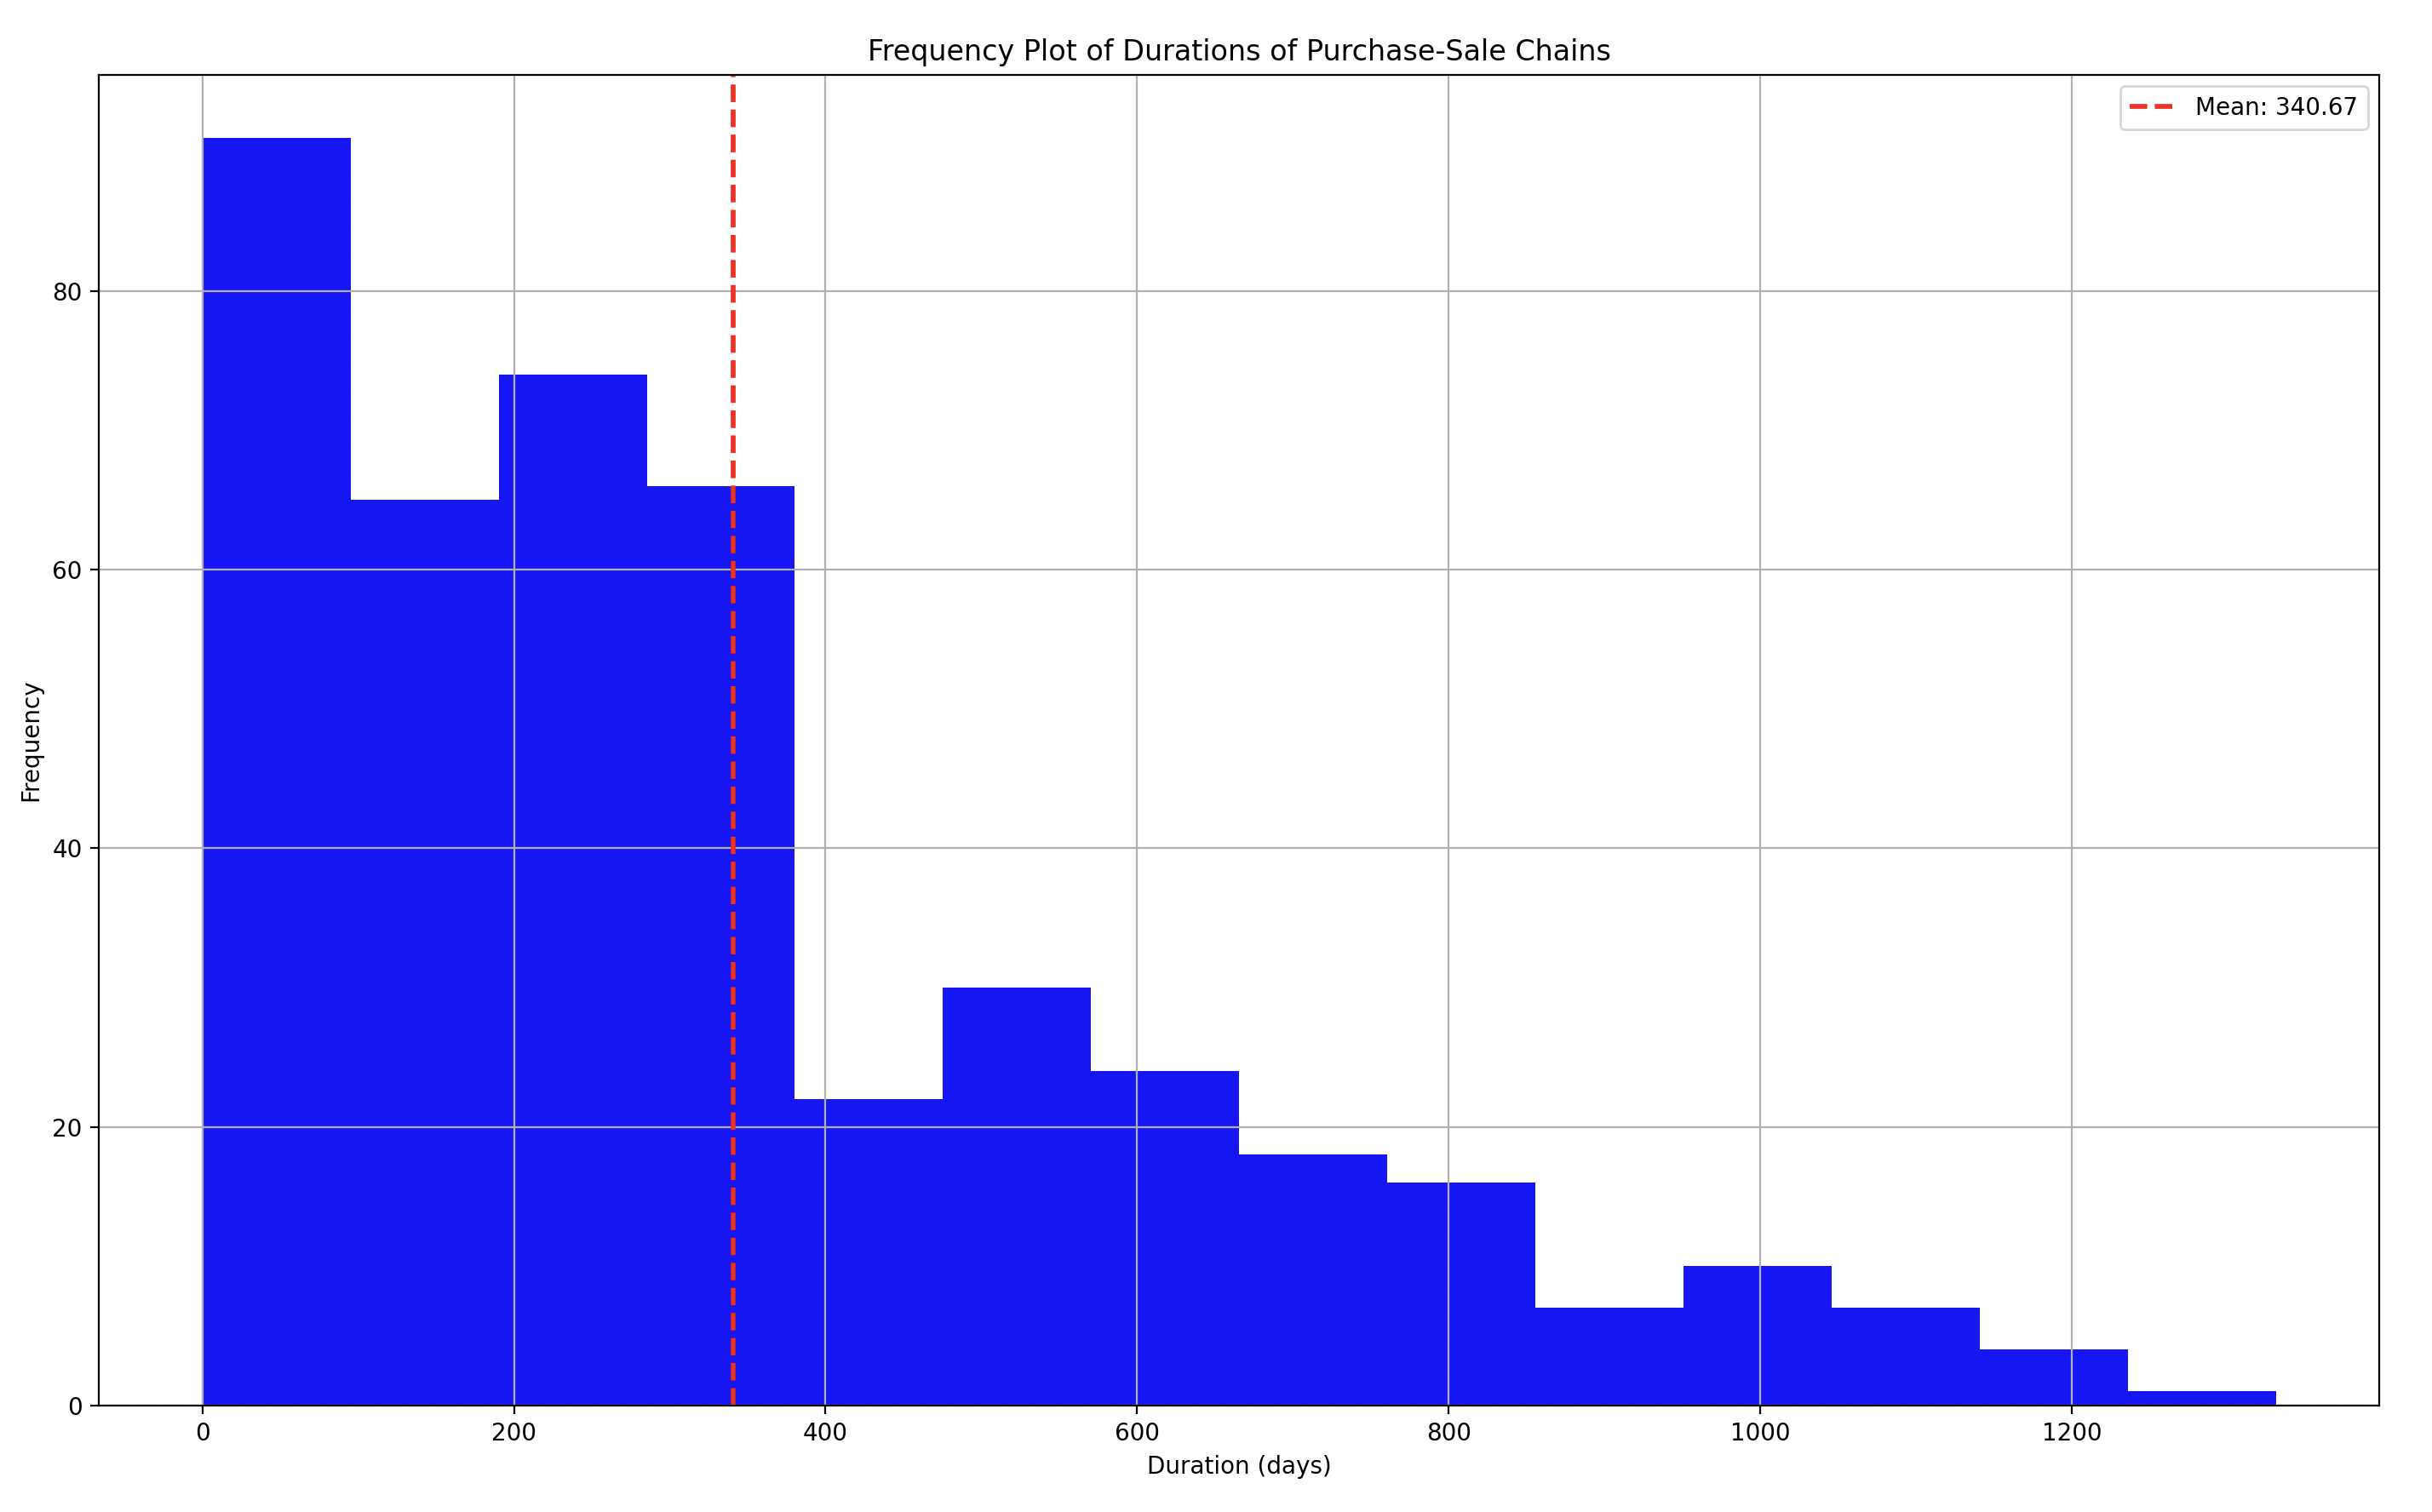
\includegraphics[width=1\textwidth]{imgs/long-du.png}
  \caption{\textbf{Frequencies of durations of long positions held by congressmen at the Senator-Ticker level} The durations are measured in days and represent the length of time between the start and end dates of each subchain. The mean duration of holding such long positions is approximately 340 days. Notably, around 65\% of these long positions are held for less than a year}
  \label{fig:erfin}
\end{figure}

\subsection{Estimating Excess Returns of Sub-sequences} \label{excess}

Estimating the excess return of the 435 sub-sequences, which were acquired following the procedure described in Section \ref{subsq}, presented a methodological challenge due to the nature of the Finance Disclosure data. The data provides only the ``minimum and maximum'' range of amounts spent on purchasing or selling each ticker on a specific day as illustrated in Table \ref{tb:rg}, rather than exact transaction amounts. To address this challenge and estimate the excess returns for each Purchase-Sale sub-sequence, the following approach was taken:

1. \textbf{Random Sampling of Transaction Amounts}: For each transaction (purchase or sale) within a sub-sequence, an amount was randomly sampled from a uniform distribution with support equal to the minimum and maximum range of the transaction amount provided in the data.

2. \textbf{Estimation of Shares Bought or Sold}: The sampled amount was divided by the volume-weighted average price (VWAP) of the stock on the corresponding transaction date to estimate the number of shares bought or sold by the congressperson.

3. \textbf{Creating Settled Pairs}: Within each sub-sequence, settled pairs of buy-sell transactions are identified. A settled pair consists of one unit of a buy transaction matched with one unit of a subsequent sell transaction. The pairing process is based on a first-in/first-out principle, meaning that stocks purchased earlier are matched first to sales, before those bought later. This ensures that the sale always occurs after the purchase. Multiple settled pairs can be created within a single sub-sequence.

4. \textbf{Computing Profit Return Rate for Each Settled Pair}: For each settled pair, the profit return rate is calculated as the relative profit or loss from the buy-sell transaction. The profit return rate is computed using the formula:
\[ \text{Profit Return Rate} = \frac{\text{Sale Price} - \text{Purchase Price}}{\text{Purchase Price}} * 100\]
where ``Sale Price'' is the price at which the stock was sold, and ``Purchase Price'' is the price at which the stock was purchased.

5. \textbf{Penalizing the Profit Return Rat with Fed Reserve Rate}: The profit return rate for each settled pair is then penalized by the average Federal Reserve Rate during the holding period of that specific pair. The holding period is defined as the time interval between the purchase date and the sale date of the settled pair. The penalized return, or ``excess return'' for each pair is calculated as:
\[ \text{Excess Return } = \text{Profit Return Rate} - \text{Average Federal Reserve Rate} \]
The Average Federal Reserve Rate represents the risk-free rate of return that could have been earned from a risk-free investment during the same holding period.

6. \textbf{Averaging Excess Returns}: The final excess return for the entire sub-sequence is computed by averaging the excess returns of all the individual pairs of settled buy-sell transactions within the sub-sequence. This approach provides a comprehensive measure of the excess return for the sub-sequence, accounting for profit ratio above the risk-free rate of return for each holding period.


By following this approach, the excess return of each sub-sequence was estimated while accounting for the limitations of the available data. Using the Federal Reserve Rate as the baseline for comparison is a more conservative approach because it represents a risk-free rate of return \citep{fed1, fed2} that is typically higher than the interest rates offered by most savings accounts. As a result, the excess return is measured against a higher baseline, potentially lowering the final estimation result and providing a more cautious assessment of the excess return earned by the congressperson.

To assist in understanding the concepts explained previously, I am presenting the estimated excess return distributions for Senator Ron Wyden’s sub-sequences involving two different companies: Applied Materials Inc. (AMAT), which provides manufacturing equipment, services, and software to the semiconductor industry, and Marriott International Inc. (MAR), a global hotel brand. These distributions were computed using the random sampling method explained earlier, where the randomness is inherited from the uniform random sampling of transaction amounts from the provided minimum and maximum ranges.
It is important to note that each sub-sequence is uniquely identified not only by the congressperson-ticker level but also by the start and end dates of the sub-sequence.
\begin{figure}[htbp]
  \centering
  \begin{subfigure}[t]{0.45\textwidth}
  \centering
  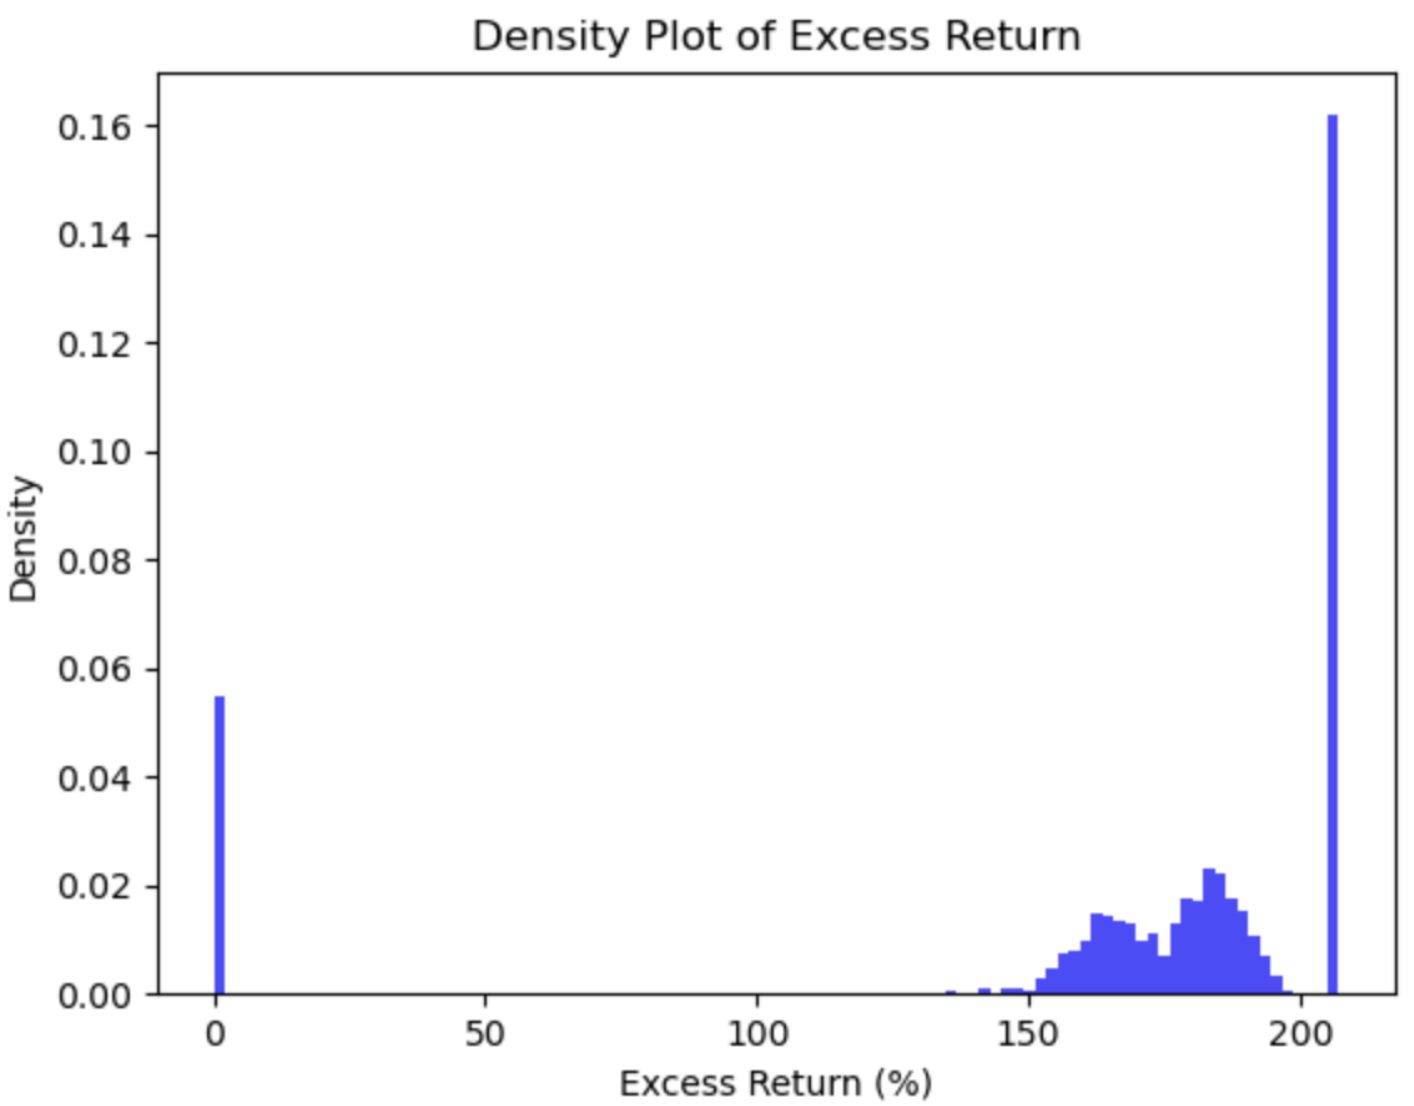
\includegraphics[width=\textwidth]{imgs/RWAMAT.png}
  \caption{Ron Wyden's excess returns from transactions involving Applied Materials Inc. (AMAT) from April 2020 to April 2021.}
  \label{fig:er_klac}
  \end{subfigure}
  \hfill
  \begin{subfigure}[t]{0.45\textwidth}
  \centering
  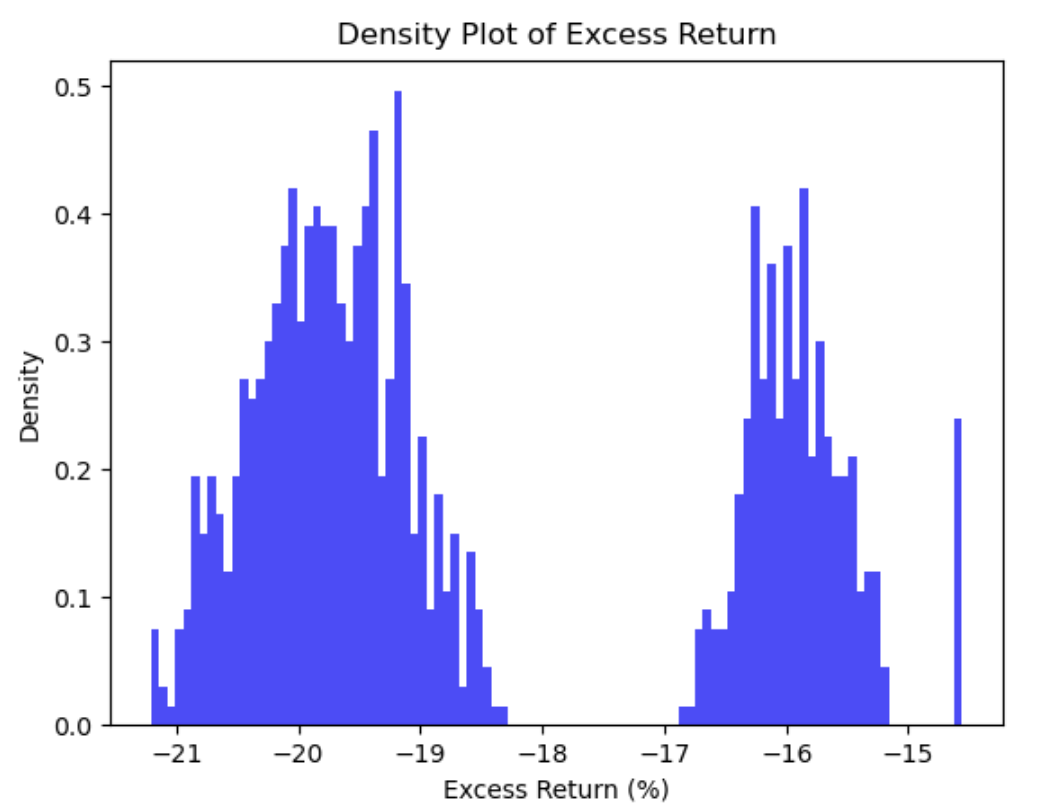
\includegraphics[width=\textwidth]{imgs/RWMAR.png}
  \caption{Ron Wyden's excess returns from transactions involving Marriott International Inc. (MAR) from May to August 2020.}
  \label{fig:er_mar}
  \end{subfigure}
  \caption{Estimated Excess return distributions of Senator Ron Wyden's transactions for AMAT and MAR
  }
  \label{fig:er}
  \end{figure}

  In Figure \ref{fig:er}, the mean of the excess return distributions for Senator Ron Wyden's sub-sequences involving AMAT and MAR are 166.30\% and -18.43\%, respectively. 
  As we can see, even the same senator sometimes achieves great excess returns while also experiencing failures. 
  In a similar vein, I collected the mean values of the excess return distributions for all 435 subsequences, which are presented in Figure \ref{fig:erfin}.

\begin{figure}[h!]
  \centering
  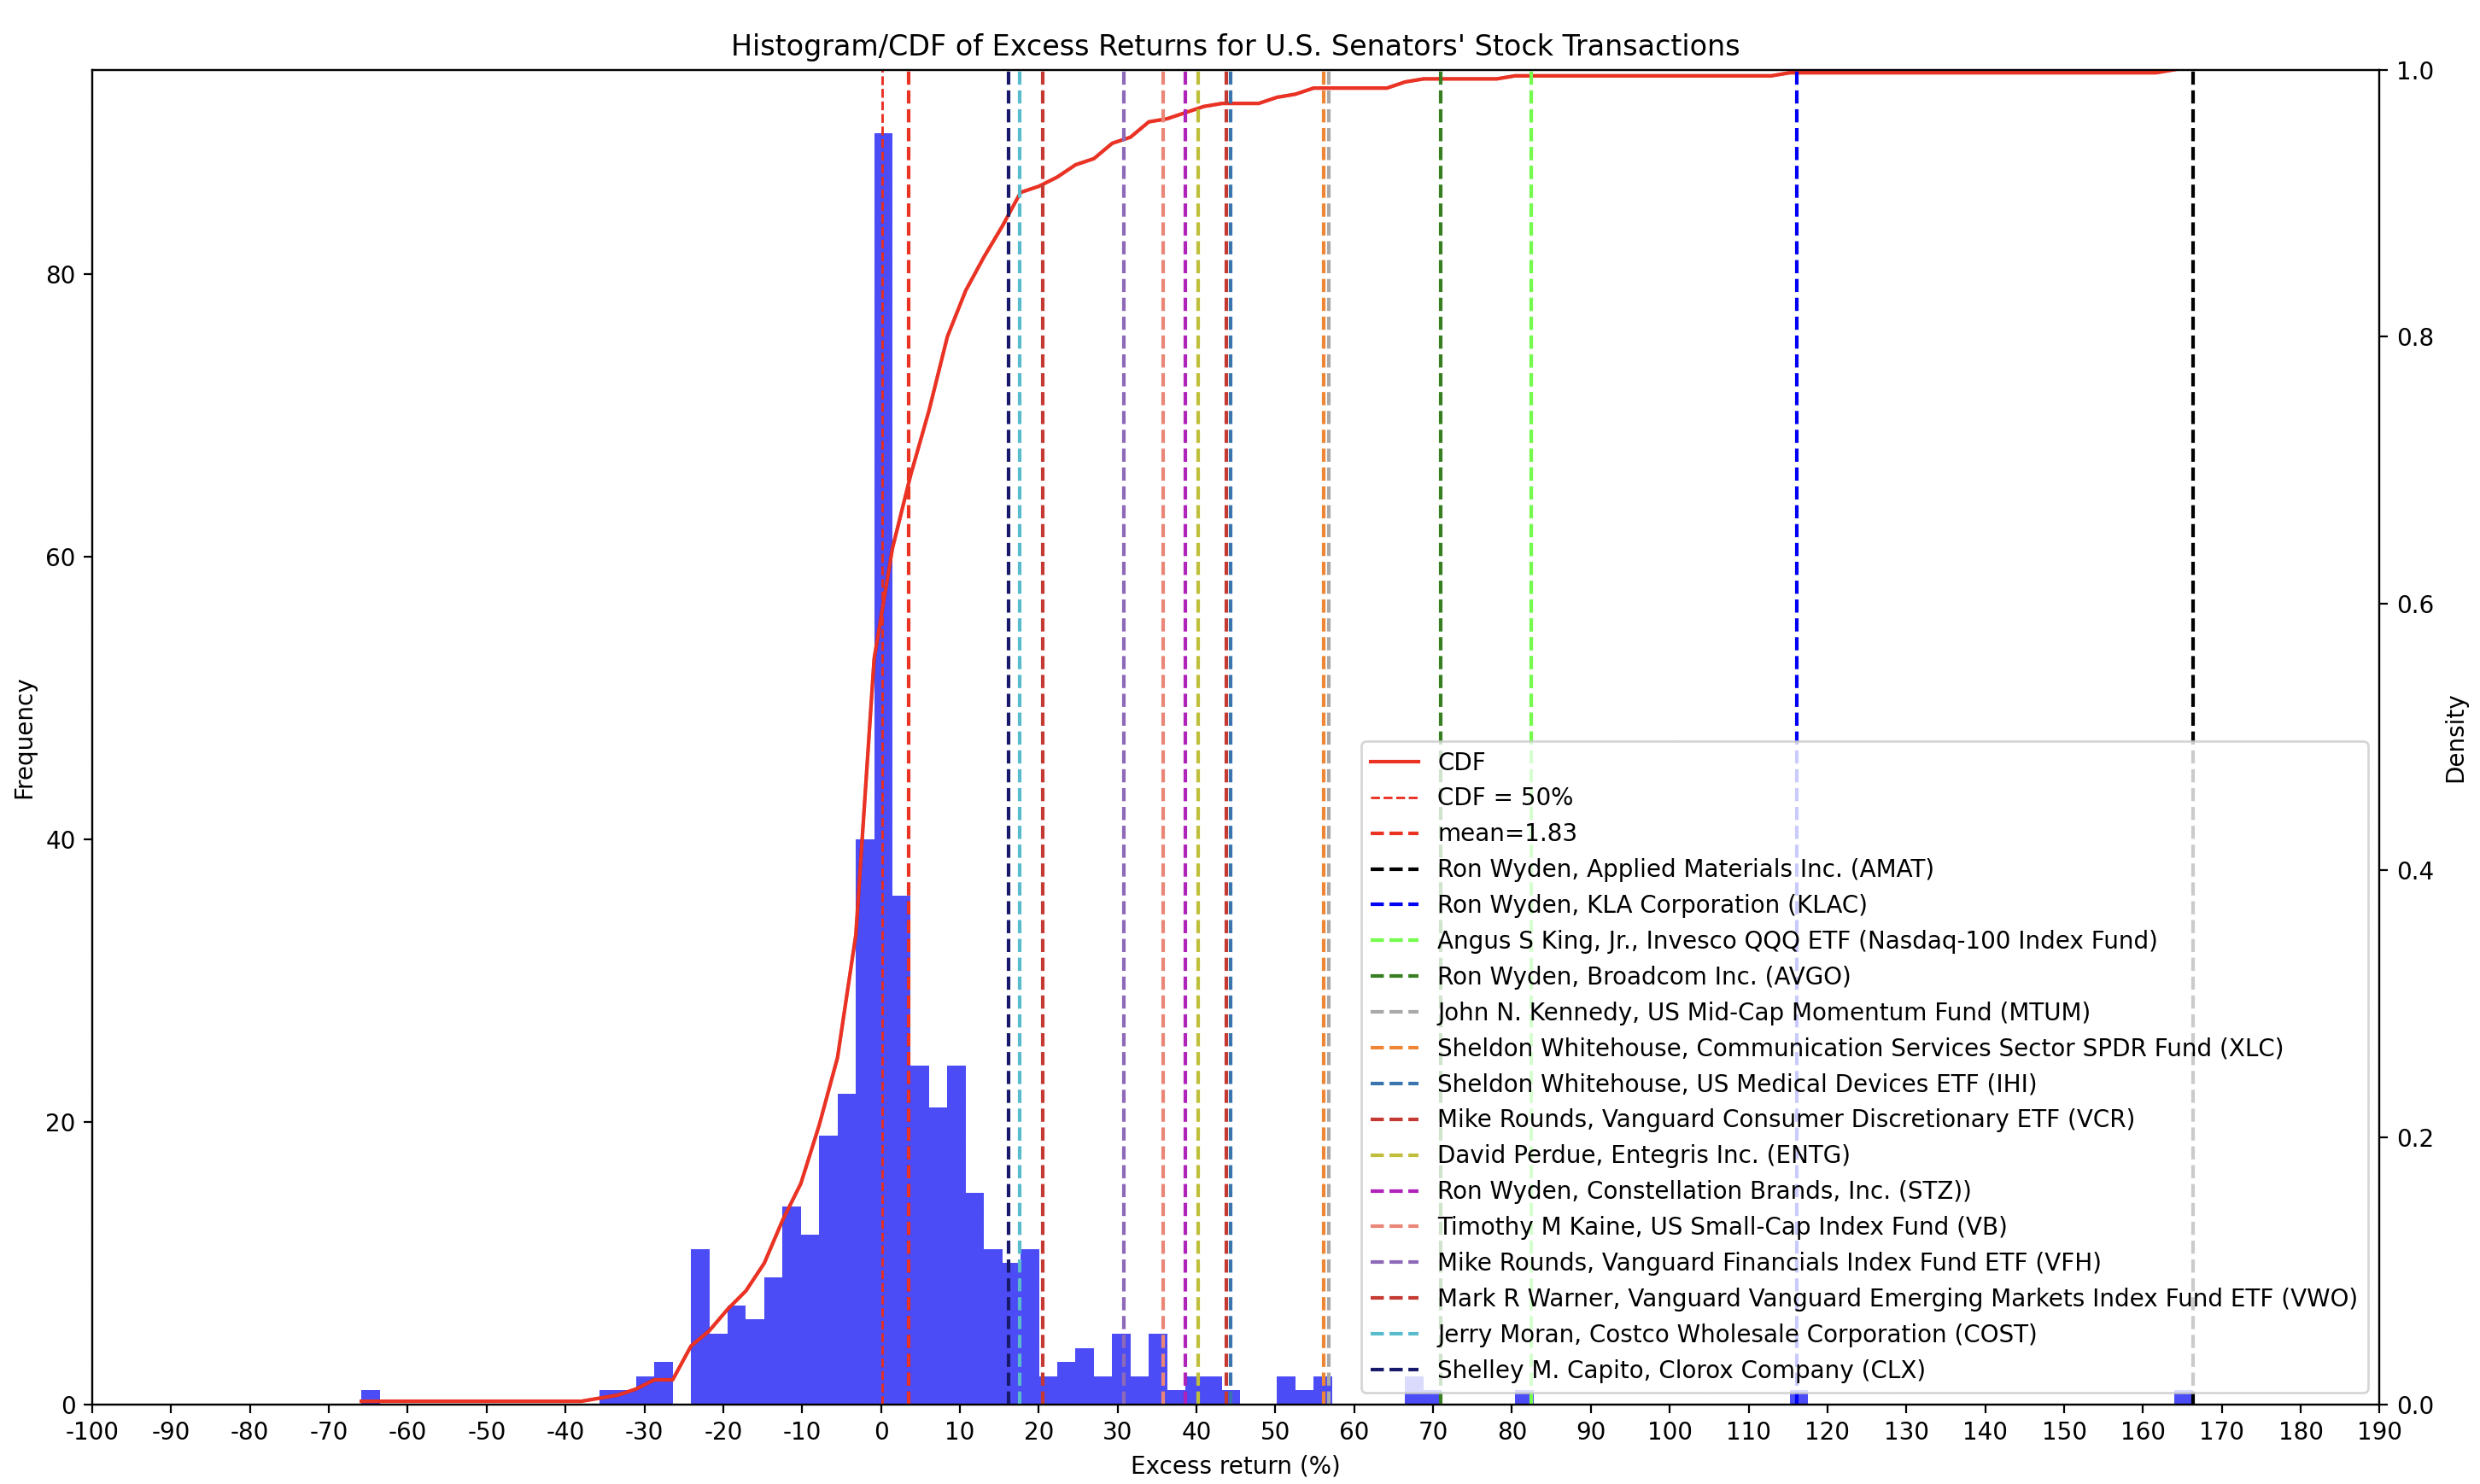
\includegraphics[width=1\textwidth, height=0.5\textheight]{imgs/ERFin3.png}
  \caption{Distribution of Senators' Mean of Estimated Excess Returns Distribution.}
  \label{fig:erfin}
\end{figure}

In Figure \ref{fig:erfin}, among the mean estimated excess returns, Ron Wyden's semiconductor-related stocks like Applied Materials Inc (AMAT), KLA Corp. (KLAC), and Broadcom Inc. (AVGO) are highly ranked, scoring from 80\% to 166\% of excess returns. These transactions have already been spotlighted by the media, as introduced in Section \ref{uct}. This suggests that this method can reveal such dubious transactions spotlighted by the media, ranking them as acquiring high-performing excess returns.

What is noticeable is that the cumulative density of the excess return distribution reaches 0.5 when the excess return is 0. It means that not all transactions of Senators are always successful, but it's more like random whether they actually acquire positive excess profit. This finding aligns more with the results from \cite{eg13} than those of \cite{zi24} and \cite{zi11}, suggesting that Senators are more like mediocre investors who align with the literature about failing individuals as investors, as explained in broad finance literature such as \cite{barberis2003}, and \cite{barber2000}.

However, one thing that is important to notice is that the distribution in Figure \ref{fig:erfin} scores a skewness of 2.804, which means the tail on the right side of the distribution is longer. This indicates that compared to the case of Senators losing money, at least in situations where they are acquiring excess return from it, they may be more related to some privileged knowledge that can back up the performance of such stock transactions. The presence of the long tail suggests that, in some cases, Senators might be involved in transactions that benefit from privileged knowledge, as \cite{eg14} suggest, which could be originating from their political connections, including connections established through Political Action Committee (PAC) donations or district-level affiliations with the firms in question.

% In conclusion, this random-sampling method suggests a way to estimate the excess return of each transaction, overcoming the range-censored nature of Financial Disclosure Data. Also, the results reassure the findings of Eggers and Hainmueller (2013) that Senators may be mediocre investors in general. However, in some cases, as Eggers and Hainmueller (2014) suggest, they might be involved in transactions that leverage privileged knowledge, as evidenced by the longer tail in the distribution of excess returns.

While the current findings provide valuable insights into the nature of congressional stock trading, it is essential to delve deeper into the fundamental relationship between congressional activities and stock transactions. In order to gain a better understanding of the underlying factors that drive congressional stock trading behavior and the potential impact of privileged information on investment decisions among lawmakers, we need to explore an approach that quantifies the predictive power embedded in the congressional activities and assesses the extent to which these activities are associated with stock transactions.

It is worth noting that this approach is not entirely novel, as \cite{eg14} have already studied the connections between congressional-related activities and the specific firm's stock transactions of a congressperson. Their research examined factors such as PAC contributions, lobbying and geographical connections based on district, and congressperson's committee membership and firm-level lobbying, to determine whether these factors could predict a congressperson's stock transactions.

Given that the innate difficulty in identifying the intention behind such transactions \citep{zi11,zi24, eg13, eg14}, due to the limited information available or the more fundamental challenge of distinguishing between a congressperson's private and public life \citep{buchanan1984}, it is essential to examine how dynamically these transactions are connected with congressional activities in terms of information. 
% Understanding to what extent these transactions are predictable would provide us with valuable insights into the potential influence of political connections and privileged information on investment decisions among lawmakers.

One possible avenue for this exploration is to represent congressional activities as a graph, which can effectively capture the complex relationships between various actors and actions \citep{g1, g2} within the legislative process. Graph-based representations are well-suited for modeling the interconnected nature of congressional activities, taking into account not only the individual actions of Congress members but also the broader context of committee memberships, lobbying efforts by firms on specific bills of their interest, the referral of bills to specific committees, and the assignment of Congresspersons to certain committees.

\cite{eg14} studied the impact of such factors, particularly committee membership and firm-level lobbying on bills,  on stock transactions at a binary level, considering whether or not this information existed for each congressperson-stock pair. However, congressional activities are more complex and interconnected, with various entities involved in these relationships simultaneously rather than in isolation. For example, multiple firms in the semiconductor industry, such as Intel, Qualcomm, Broadcom, Apple, and IBM, participate in lobbying efforts for bills related to their sector, like the CHIPS Act (H.R.4346 117th Congress) or FABS Act (S.2107 117th Congress). These activities are governed by specific congresspeople within particular committees, and all this information collectively can forms the detailed context in which a congressperson transacts stock.

In addition, as explained in Section 2.1, a congressperson's securities transactions are not limited to individual firm levels. In fact, 60\% of these transactions involve exchange-traded funds (ETF) or mutual funds that target a wide range of specific industries such as wireless communication, medical devices, or mid-cap or small-cap companies. Therefore, the full context of a congressperson's stock transactions extends beyond individual companies to encompass broader industry trends and movements.

In light of this, the next section will introduce a newly compiled dataset that captures congressional activities as a whole, in the form of graph-structured data. I will then demonstrate how this graph-structured data can be useful, for example, by directly computing the similarity between a committee's industry-level specialization and the industry-level distribution of a congressperson assigned to that committee in Section \ref{sec:ce}. Additionally, I will present a method for modeling the predictive task, which can directly take graph-structured data as input using Graph Neural Networks in Section \ref{sec:gnn}. 
An array of analyses using graph-structured data will enhance our comprehension of the intricate relationships between congressional activities and stock transactions. This approach will offer more profound insights into the potential influence of privileged information acquired through congressional activities on lawmakers' investment decisions.





% In this context, Graph Neural Networks (GNN) emerge as a promising technique to analyze such graph-based representations of congressional activities. GNNs are designed to learn meaningful patterns from complex graph structures, enabling them to uncover hidden relationships and interactions among nodes in the graph. This ability to capture and process the topological information of graphs allows GNNs to effectively model the interconnected nature of congressional activities and their potential influence on stock trading decisions.

% In the following sections, we will outline the methodology and preliminary results of this novel application of GNN in studying the predictive power of congressional activities in relation to stock trading. By leveraging the capabilities of GNN, we aim to provide a deeper understanding of the role of political connections and privileged information in shaping lawmakers' investment behavior and shed light on the extent to which such factors may impact the performance of their stock transactions.

% % As shown in Figure 5, it appears that Senator Ron Wyden may have access to legislative information regarding bills that could impact both the semiconductor and hospitality industries. During the 117th Congress, which coincides with Senator Ron Wyden's transaction involving AMAT, the company lobbied for two bills: S.2107 FABS Act and S.749 American Innovation and Jobs Act. Both bills include provisions that provide subsidies to the semiconductor industry. Additionally, during the 117th Congress, which overlaps with Senator Ron Wyden's transaction involving MAR, the company lobbied for two bills: S.477 Hospitality and Commerce Job Recovery Act of 2021, which extends tax credits to assist the hospitality and restaurant industry, and S.1519, which grants awards to hotel owners. It is worth noting that this legislative information likely flowed from the firms' lobbying efforts directed towards the Senate Finance Committee, which oversees the bills listed.
% \begin{figure}[htbp]
%   \centering
%   \begin{subfigure}[t]{0.45\textwidth}
%   \centering
%   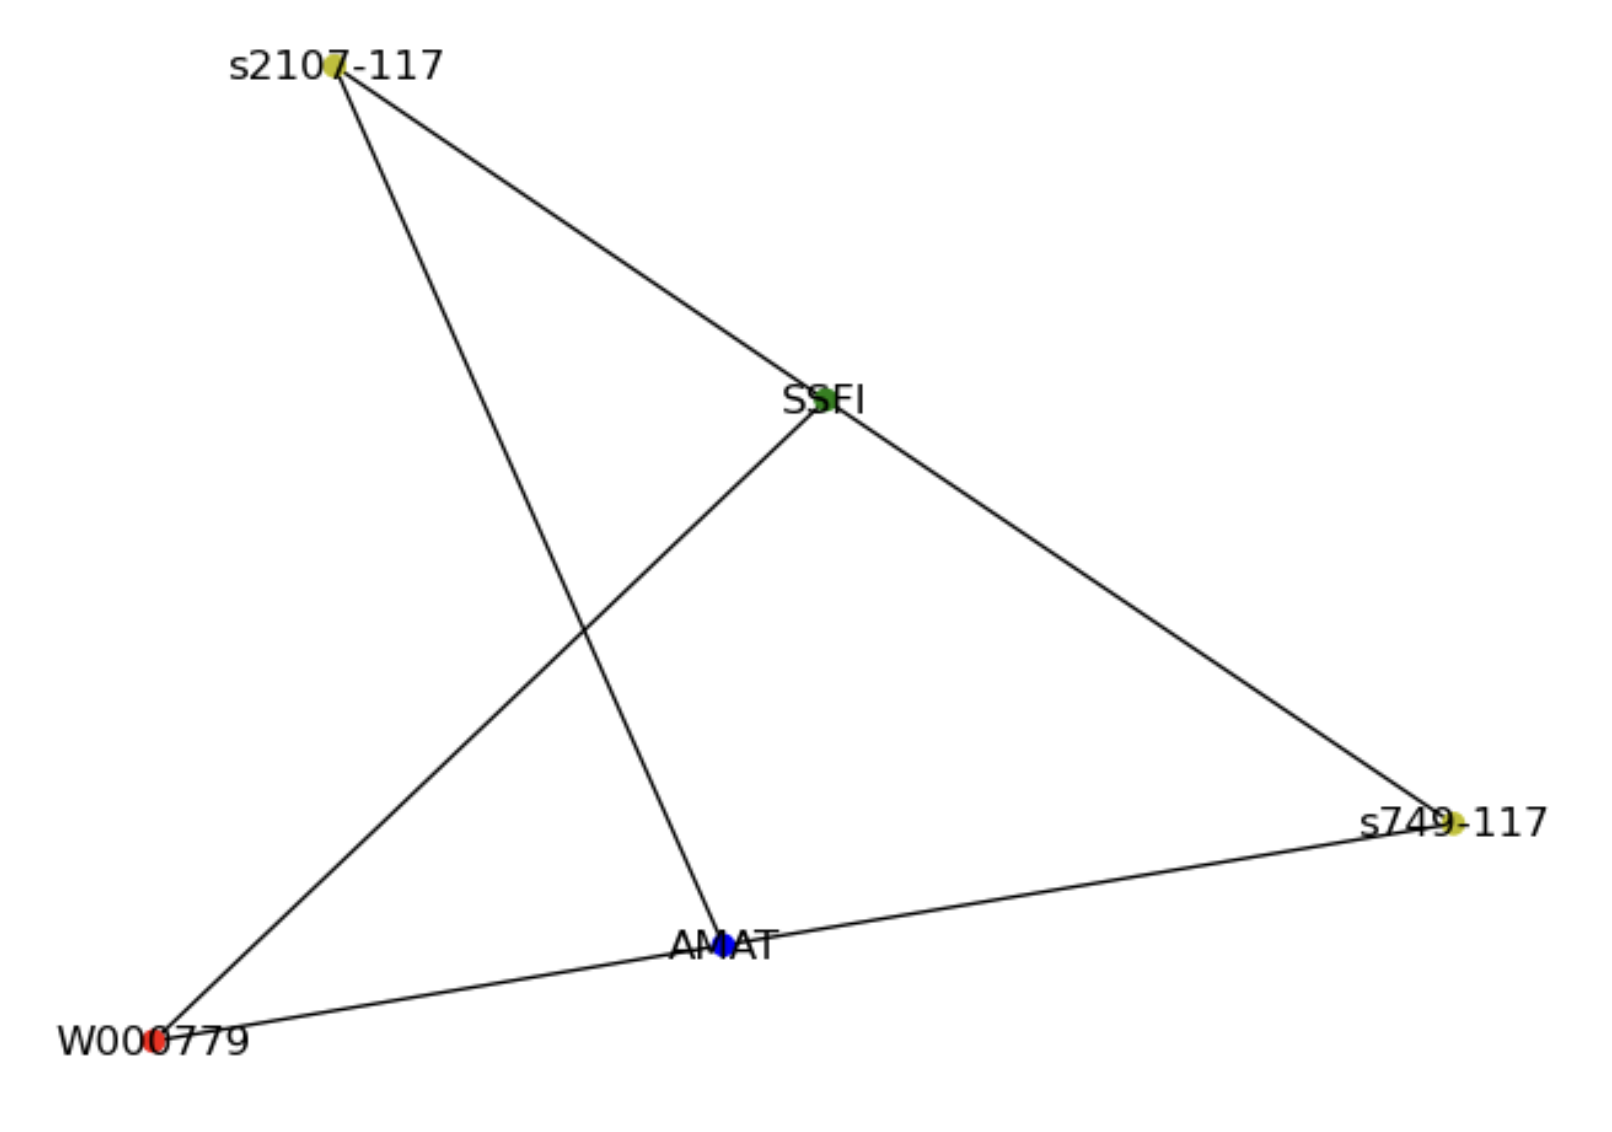
\includegraphics[width=\textwidth]{imgs/AMATDAG.png}
%   \caption{Subgraph extracted from the congressional network that is in close proximity to Senator Ron Wyden's purchase or sale transaction involving AMAT.}
%   \label{fig:er_klac}
%   \end{subfigure}
%   \hfill
%   \begin{subfigure}[t]{0.45\textwidth}
%   \centering
%   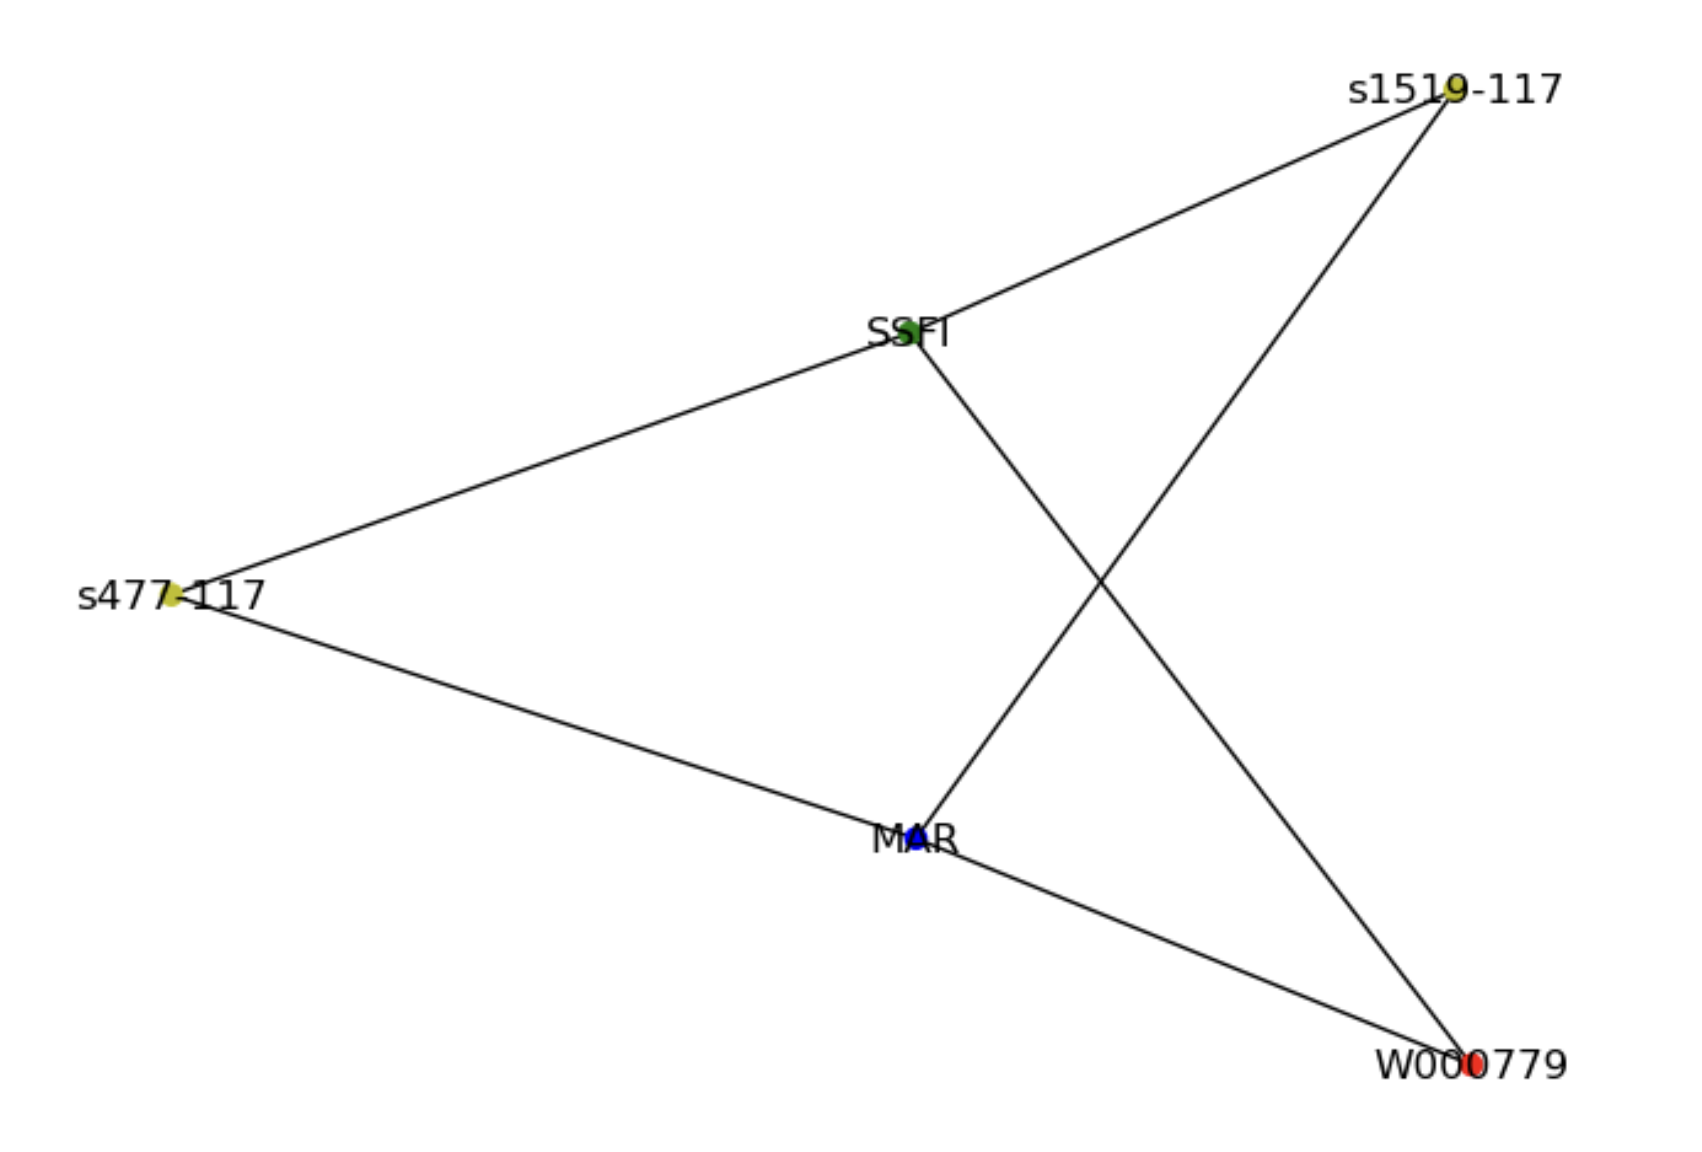
\includegraphics[width=\textwidth]{imgs/RWMAR2.png}
%   \caption{Subgraph extracted from the congressional network that is in close proximity to Senator Ron Wyden's purchase or sale transaction involving MAR.}
%   \label{fig:er_mar}
%   \end{subfigure}
%   \caption{Potential Access to Legislative Information by Senator Ron Wyden Regarding Bills Impacting Semiconductor and Hospitality Industries during the 117th Congress
%   }
%   \label{fig:er2}
% \end{figure}




% Based on both Figure \ref{fig:er} and Figure \ref{fig:er2}, we can conclude that although Senator may have access to legislative information about certain industries, it is not always possible to profit from it due to external factors that the legislative information from congressional activity cannot explain. This example provides suggestive evidence as to why a simple excess return approach cannot provide a persuasive argument that proves or disproves the existence of insider trading.  

% Finally, I provide a distribution of the mean estimated excess return for each (Senator, Ticker) pair in Figure \ref{fig:erfin}. The plot shows that only a few transactions are acquiring abnormal positive profits over 50\%, and almost half of them record negative returns. This statistic is consistent with the findings reported by \cite{eg13}, which suggests that there is little evidence of systematic abnormal returns for members of Congress. 

% However, thanks to the current approach that delves more into the Senator and Ticker level, we can conclude that it is hard to deny that a few transactions are acquiring abnormally high returns connected to the relevant legislative information that is accessible during congressional activity.


% \subsection{Committees: A Channel for Legislators to Acquire Industry-Specific Information}\label{comm}
% Based on multiple anecdotes and observations, I hypothesize that legislators acquire industry-specific information from their committee assignments that they may use for personal investments. For example, Senator Ron Wyden's semiconductor stock transactions involving multiple tickers in the same industry, such as AMAT, AVGO, and KLAC, can be explained by this hypothesis. These companies lobbied for bills relevant to the semiconductor industry, and the industry-level preferences and possible impacts of legislation on the semiconductor industry were aggregated in the Senate Finance Committee, which oversees such bills. As a member of the Senate Finance Committee, Ron Wyden acquired a more detailed understanding of how vital these bills were to the industry, and may have timed his transactions accordingly.
% I also provide an additional illustration that shows how the preferences of the semiconductor industry were focused on the Senate Finance Committee during the 117th Congress in Figure \ref{fig:semi}. The NAICS code 334413 indicates Semiconductor and Related Device Manufacturing, which involves companies such as Qualcomm (QCOM), Intel (INTC), IBM (IBM) and Advanced Micro Devices (AMD), lobbying for bills such as the American Innovation Act (S2992-117) and FABS Act (S2107-117) that are closely related to the subsidization of semiconductor manufacturing facilities. Relevant companies such as Apple Inc. and IBM, with NAICS codes of 334220 Wireless Communications Equipment Manufacturing and 334118 Computer Equipment Manufacturing, respectively, are direct customers of these semiconductor chips for manufacturing smartphone and computer hardware. The bills in which these companies have an interest are assigned to the Senate Finance Committee as well.



% As another example, I provide how the Senate Banking Committee (SSBK) serves as a channel for different financial companies to project their lobbying interests over bills. NAICS codes starting from 52 generally relate to the financial industry in Figure \ref{fig:ssbk}. For instance, Wells Fargo (WFC) and AIG are lobbying for H.R.1996 - SAFE Banking Act of 2021, which prohibits a federal banking regulator from penalizing a depository institution for providing banking services to a legitimate cannabis-related business. Capital One Inc. (COF) and MetLife Inc. (MET) are lobbying for H.R.4616, which allows for the transition of certain financial contracts away from the London Interbank Offered Rate (LIBOR). These bills are all funneled through the Senate Banking Committee, thus a committee member of SSBK is more likely to be equipped with in-depth knowledge of the financial industry.

% \subsection{Causal Quantity of Interest: Effect of Committee Membership on Trading Behavior}

% In Section \ref{comm}, illustrative examples were provided to suggest that committee assignments can influence a congressman's financial behavior by utilizing industry-level specialized information funneled through the committee. Building on this insight, I propose a Directed Acyclic Graph (DAG) in Figure \ref{fig:dag} that captures the hypothesized causal relationships between committee assignments, congressional knowledge, and financial behavior. Specifically, I expect that Congressional Knowledge before joining a committee will act as a confounder, influencing both the committee assignment and financial behavior. After joining the committee, Congressional Knowledge will mediate the effect of the committee assignment on financial behavior. At the outcome level, I expect that the industry distribution of a senator's portfolio after joining the committee will become more similar to that of the committee. The industry distribution of the committee will be evaluated by examining the firms' industry distribution lobbying for bills assigned to that committee.

% \begin{figure}[h]
%   \centering
%   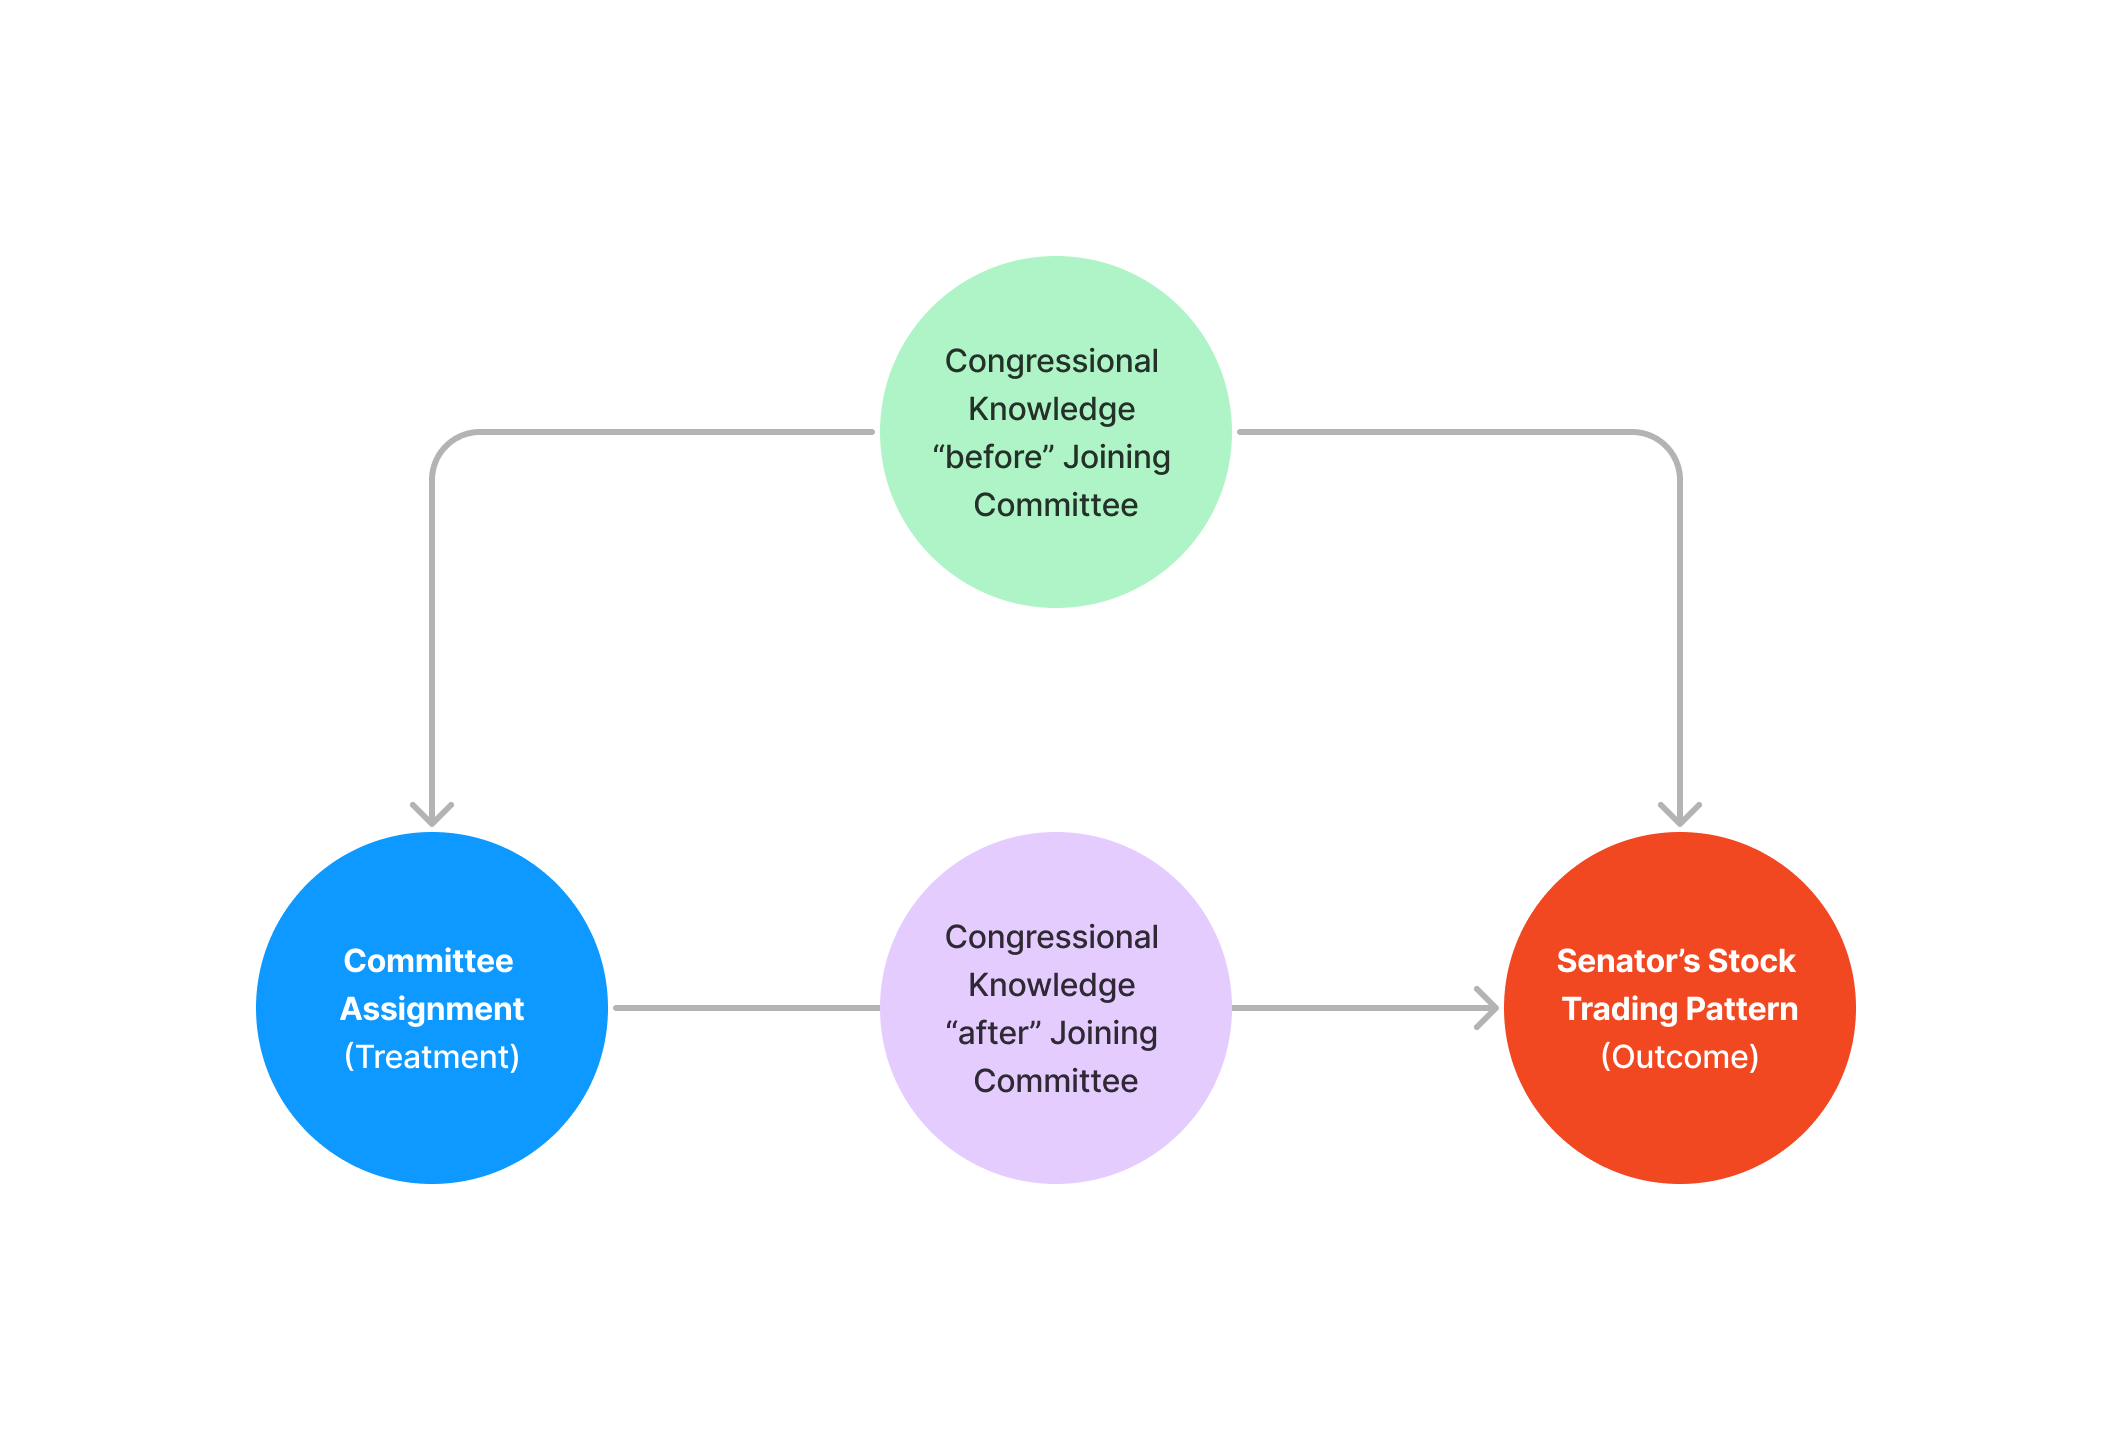
\includegraphics[width=1\textwidth]{imgs/causaldag.png}
%   \caption{Causal diagram that demonstrates how committee assignments affect the congressmen's transaction behavior}
%   \label{fig:dag}
% \end{figure}

% To justify the measurement of the outcome variable as a similarity between the industry-level distribution of a senator's stock trading portfolio and that of the committee, I analyzed the stock trading portfolio and its NAICS code distribution for Senator Ron Wyden, as well as those of the Senate Finance Committee (SSFI) and Senate Banking Committee (SSBK) over the 117th Congress, as shown in Figure 8. I calculated the discrete probability distribution of the collection of 2-digit level NAICS codes for each entity, and used cross-entropy to measure the similarity between the Senator and each committee's NAICS code distribution. The results indicate that the cross-entropy between Senator Ron Wyden's NAICS code distribution and that of SSFI is 0.71, while the cross-entropy between Senator Ron Wyden's NAICS code distribution and that of SSBK is 3.31. 
% A smaller cross-entropy value signifies a more similar distribution, indicating that Senator Ron Wyden's NAICS code distribution is closer to that of SSFI than SSBK. This supports the hypothesis that committee assignments influence a senator's investment choices, as Ron Wyden is a member of SSFI but not a member of SSBK.

% \begin{figure}[ht]
%   \centering
%   \begin{subfigure}[b]{0.3\textwidth}
%     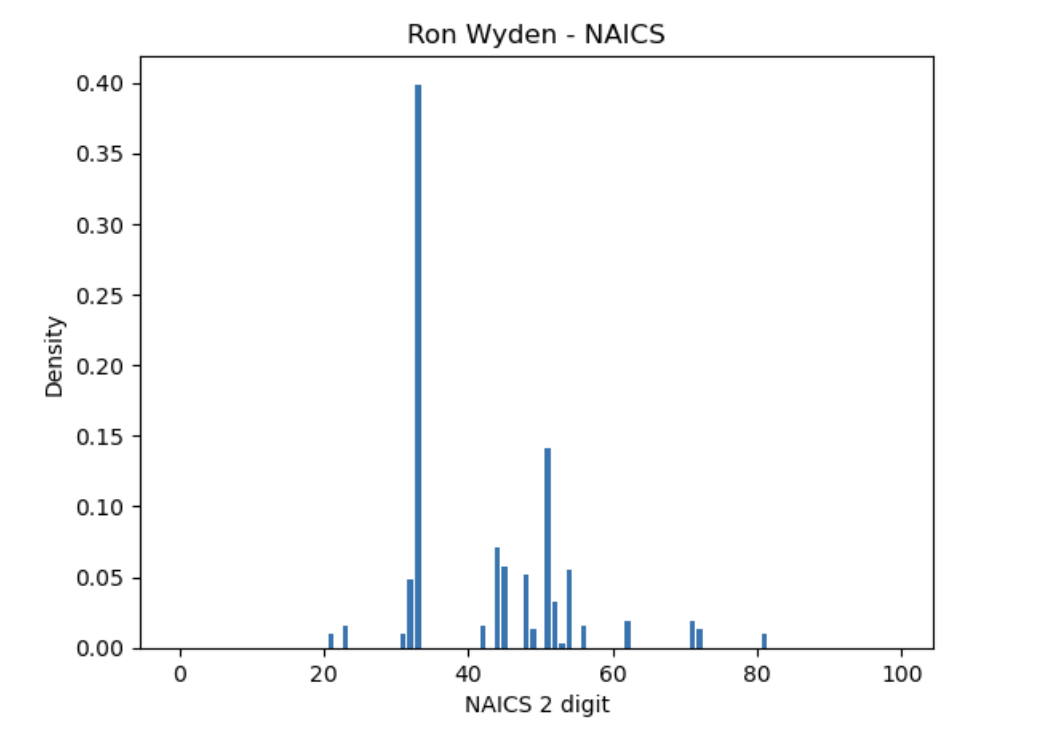
\includegraphics[width=\textwidth]{imgs/naics1.png}
%     \caption{NAICS code distribution of Senator Ron Wyden's stock portfolio over the 117th Congress.\\}
%     \label{fig:subfig1}
%   \end{subfigure}
%   \hfill
%   \begin{subfigure}[b]{0.3\textwidth}
%     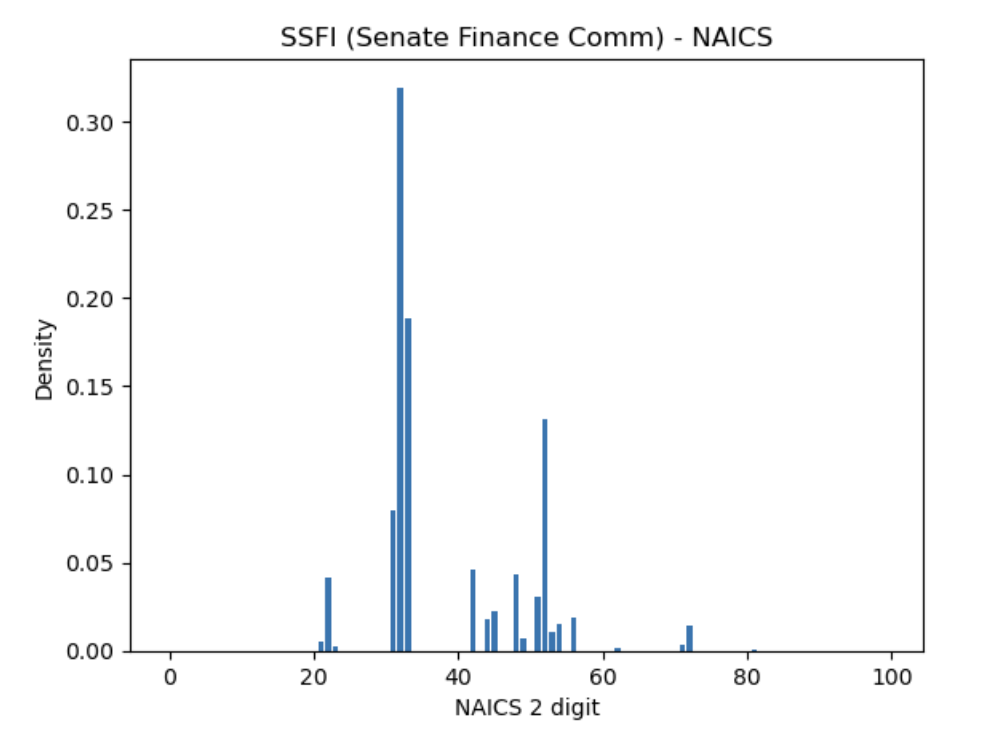
\includegraphics[width=\textwidth]{imgs/naics2.png}
%     \caption{NAICS code distribution of firms lobbying for bills assigned to Senate Finance Committee in the 117th Congress.}
%     \label{fig:subfig2}
%   \end{subfigure}
%   \hfill
%   \begin{subfigure}[b]{0.3\textwidth}
%     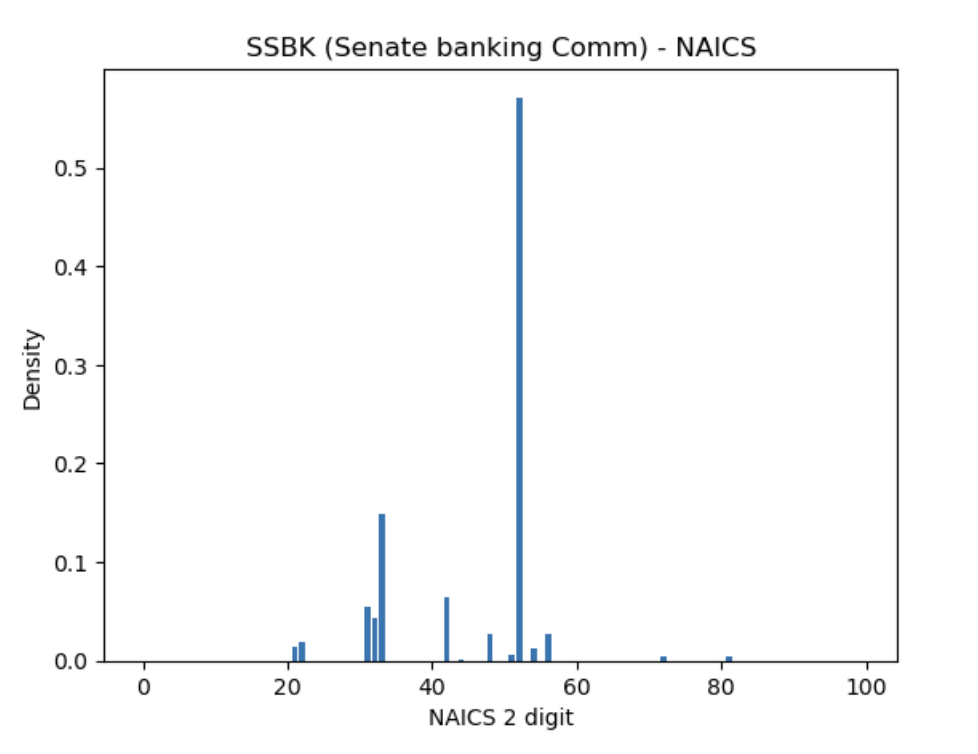
\includegraphics[width=\textwidth]{imgs/naics3.png}
%     \caption{NAICS code distribution of firms lobbying for bills assigned to Senate Banking Committee in the 117th Congress.}
%     \label{fig:subfig3}
%   \end{subfigure}
%   \caption{NAICS code distribution of Senator and Committees.}
%   \label{fig:mainfig}
% \end{figure}

% Therefore, I conclude that by estimating the causal effect of committee assignment on the cross-entropy between committees and senators, we can determine whether the information funneled through committee in congressional activity, after joining such committee, affects congressmen's trading behavior or not, provided that we properly control for the level of congressional knowledge before joining the committee.

% Then there exists a remaining question: how to measure congressional knowledge ``before'' joining a committee? Before proceeding, I assume that the congressional network $G$ described in Section \ref{data} is a comprehensive source of relevant information, meaning that it is sufficient to satisfy the backdoor-adjustment criterion for correctly estimating the causal effect of committee assignment on the outcome. However, although $G$ includes this sufficient information, we need to separate the congressional knowledge ``before'' and ``after'' joining the committee. Additionally, there is another challenge: $G$ is a discrete object that cannot be directly used in any model to estimate the quantity of interest in its raw format. To overcome these challenges, I suggest using Graph Neural Network (GNN) to learn the corresponding numerical representations that correspond to the congressional knowledge ``before'' joining the committee.

% Figure \ref{fig:gnn} briefly illustrates how Graph Neural Networks (GNN) work. Given an original graph whose nodes are represented as $x_i$, we learn the corresponding numeric representation of $x_i$, which is $h_i \in \mathbb{R}^k$, by aggregating information from the neighboring nodes. In the case of $x_2$, for example, we aggregate information from its neighbors $(x_1, x_5, x_6)$ to generate $h_2$. Over the layers of the neural network, this process is repeated until we learn the representation that achieves the best performance in the downstream task, in this case estimating the potential outcomes.
% \begin{figure}[h]
%   \centering
%   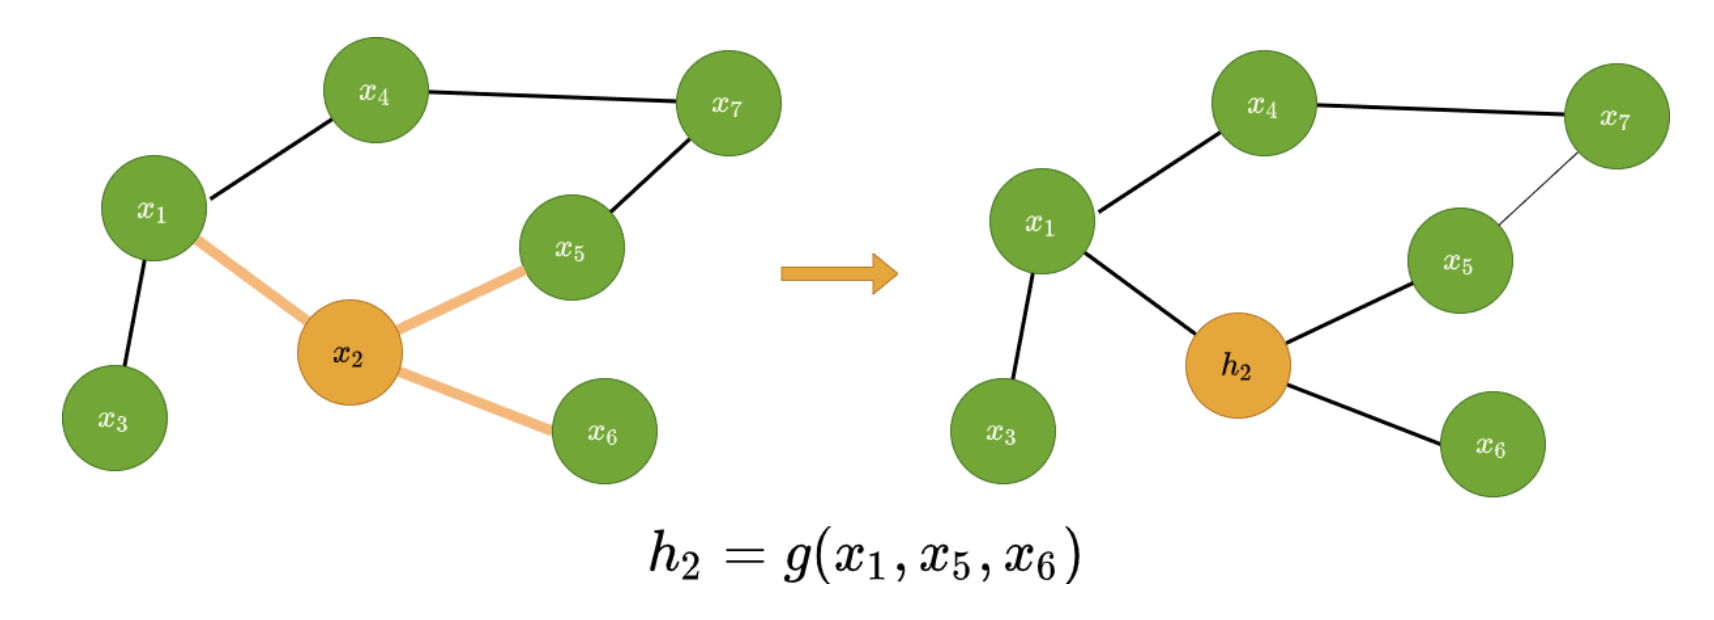
\includegraphics[width=1\textwidth]{imgs/howGNN.png}
%   \caption{A brief illustration of how Graph Neural Networks (GNN) work is presented below. The diagram is borrowed from \url{https://theaisummer.com/gnn-architectures/}}
%   \label{fig:gnn}
% \end{figure}

% Then general idea to learn the representation of congressional knowledge before joining a committee is to prepare additional nodes that encode the information of each congress, and learn the joint representation that aggregates a senator's information and those of congresses before joining such committees, as illustrated in Figure \ref{fig:daggnn}.

% \begin{figure}[h]
%   \centering
%   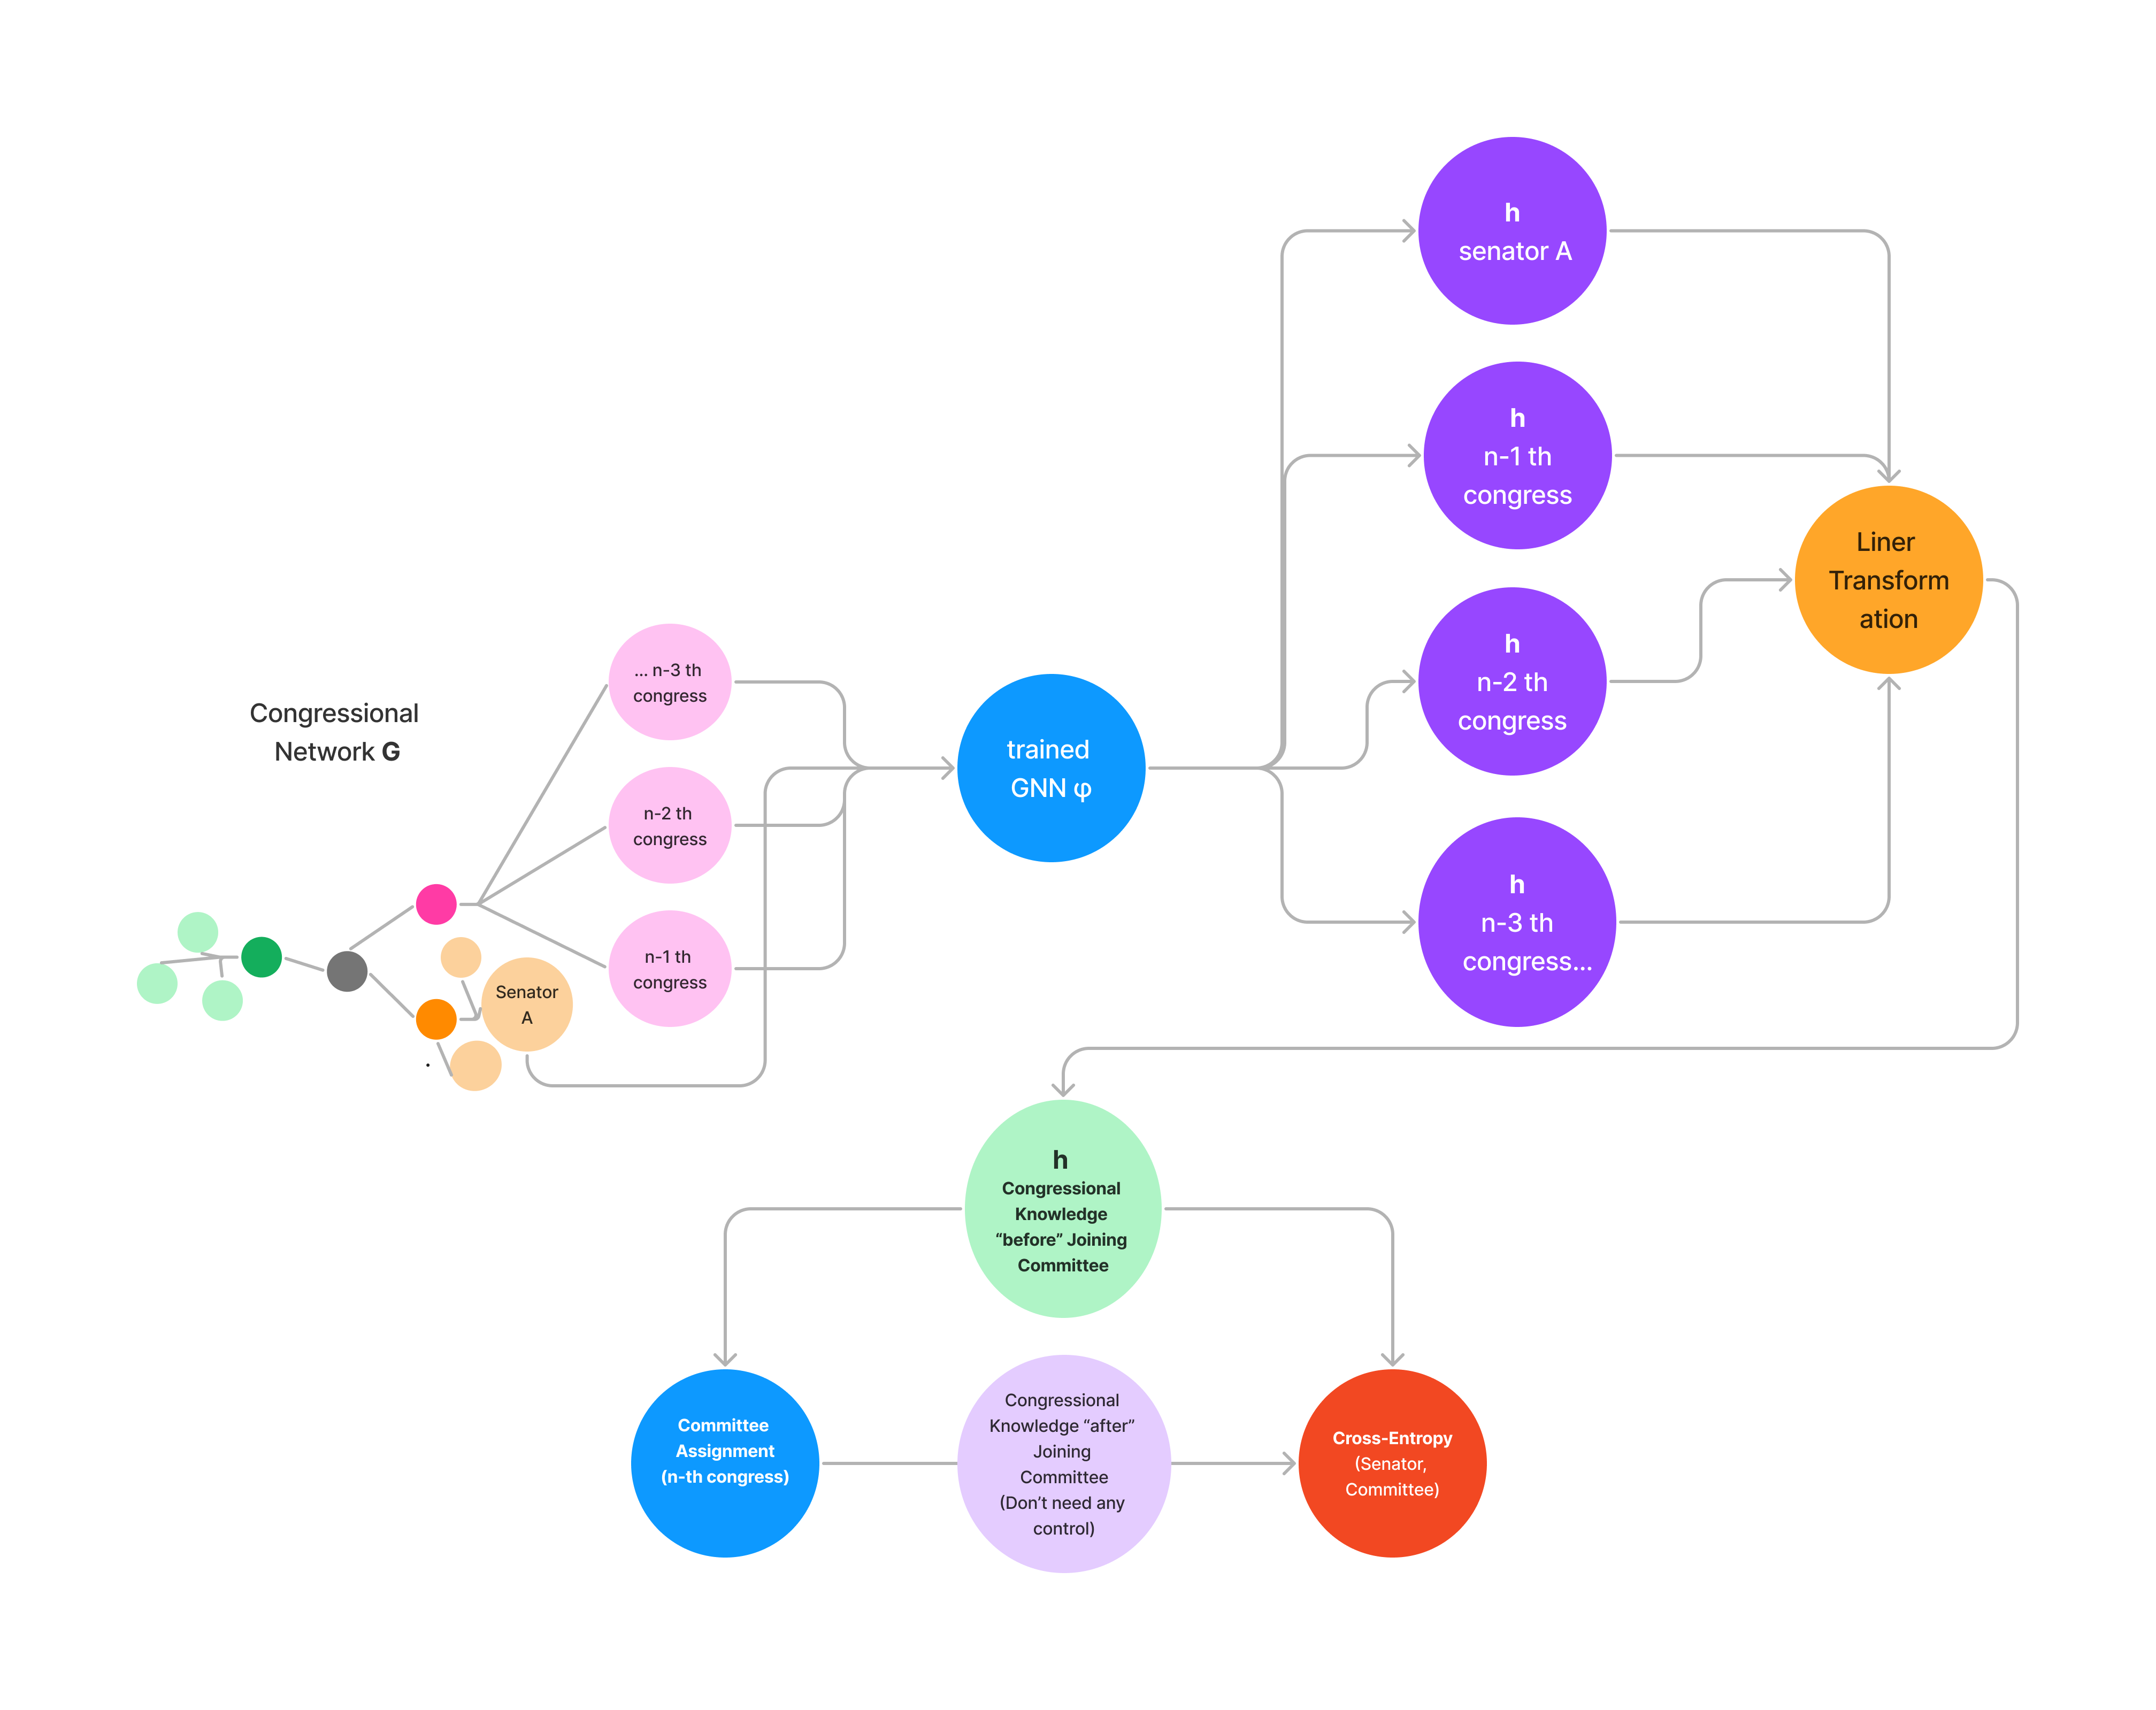
\includegraphics[width=1\textwidth]{imgs/daggnn.png}
%   \caption{An illustration of how to utilize GNN to learn the numeric representation of congressional knowledge before joining a committee}
%   \label{fig:daggnn}
% \end{figure}

% \subsection{Estimation of CATE}

% Finally, by denoting the learned representation of Senator $i$'s congressional knowledge before joining the committee at time $t$ as $h_i = \phi_{GNN}(i, G; t-1)$, the study can estimate the conditional average treatment effect (CATE) by learning estimators for both $\mu_0(h_i) \equiv \mathbb{E}\left[Y_i \mid H=h_i, T_i=0\right]$ and $\mu_1(h_i) \equiv \mathbb{E}\left[Y_i \mid H=h_i, T_i=1\right]$, and using the formula $\text{CATE}(h_i) = \mu_1(h_i) - \mu_0(h_i)$. This allows the study to estimate the effect of committee assignment on the similarity between a Senator's and the assigned committee's NAICS code distribution, while controlling for potential confounders through the learned representation $h_i = \phi_{GNN}(i, G)$.
% For the estimator $\mu_0(h_i)$ and $\mu_1(h_i)$, the study will use the Treatment Agnostic Regression Network (TARNet) \citep{tarnet}, which extends T-learners \citep{tlearner} with additional layers of neural networks that learn a shared representation of $h_i = \phi_{GNN}(i, G; t-1)$ for the treatment and control groups in a balanced way. By doing so, the neural network can effectively perform its regression task to estimate CATE, even though $h_i$ is asymmetrically distributed between the treatment and control groups.

% \begin{figure}[h]
%   \centering
%   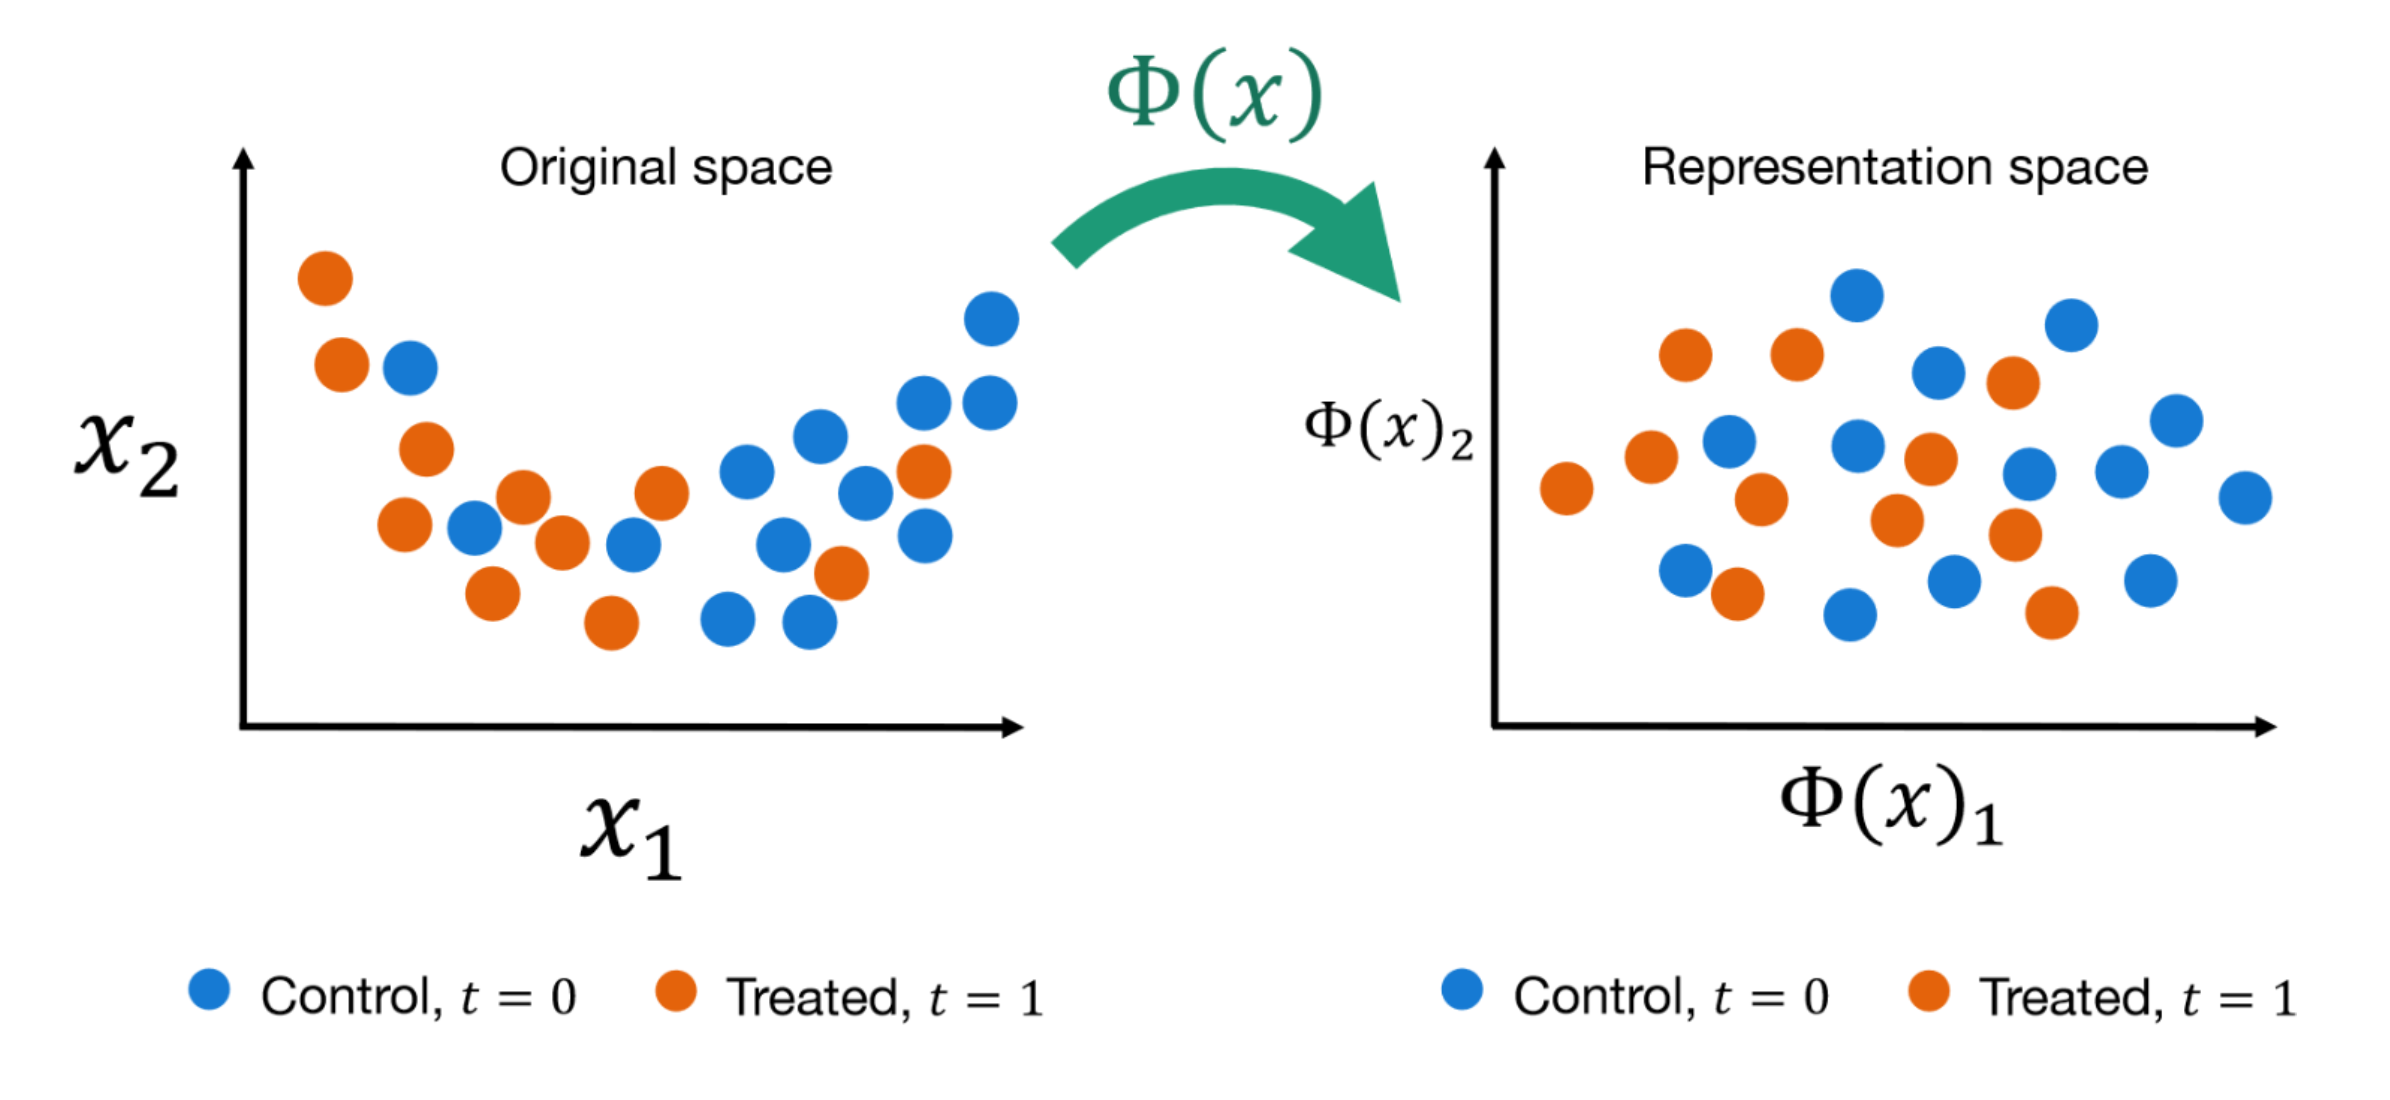
\includegraphics[width=1\textwidth]{imgs/balancing.png}
%   \caption{An illustration of how balancing works using TARNet's shared representation. The diagram is borrowed from \citep{koch}.}
%   \label{fig:bal}
% \end{figure}

% The necessity of adding an additional balancing layer is quite straightforward. For a given committee, the number of senators assigned to that committee is relatively small compared to those who are not assigned to it. By incorporating additional layers with appropriate loss functions, it is expected that $h_i$ will be mapped into a more balanced space, where $\phi_{\text{balancing}}(h_i; T=0)$ and $\phi_{\text{balancing}}(h_i; T=1)$ are evenly distributed as illustrated in Figure \ref{fig:bal}. 

% \subsection{Evaluation of CATE}
% There are a total of 62 different committees, and CATE is estimated for each committee separately using the transaction information of 95 Senators across various congresses, spanning from the 114th to the 117th Congress. By evaluating these CATE values, the paper aims to quantitatively assess how committee assignments heterogeneously affect Senators' behavior across committees and among the Senators themselves.
% \section{Conclusion and Contributions}

% The paper aims to make two main contributions. Firstly, it substantively proves the existence of insider trading by explicitly showing that committee membership changes affect Congressmen's investment behavior to become similar to the information available from the committee. Secondly, it demonstrates a novel methodological approach to estimate causal quantities using graph-structured data by leveraging representation learning via Graph Neural Network. Therefore, the paper proposes a model and learning scheme that combines a Graph Neural Network and meta-learners to learn CATE, conditioning on the output of the Graph Neural Network. 


% % From the previous section on data, I described a large network that captures congressional activities in general. Let me denote this network as $G$, which includes different types of nodes and edges as explained in Tables \ref{tab:nodes} and \ref{tab:edges}\footnote{Formally, this type of network that includes different types of nodes and edges is called a heterograph}. 

% % After analyzing the initial results, I have decided to investigate how committee membership impacts the trading behavior of Congressmen. Typically, each Congressmen is assigned to one or two committees, which are responsible for overseeing the legislation on a specific topic or bill. Companies that have a stake in the legislation have varying levels of interest and involvement, and this relationship is illustrated in Figure 2.

% % If the Lobbyview data is merged with my transaction data, it would be able to capture the 
% %  between bills, committees, companies, and Congressmen. Since these interactions can be represented as structured graph data, I plan to use a Graph Neural Network (GNN) for predictive analysis. The GNN will predict a Congressmen's investment in a specific stock using a graph network that includes information on bills, companies lobbying on those bills, committees with jurisdiction over those bills, and the Congressmen assigned to those committees.

% % A Graph Neural Network (GNN) is a type of neural network that can analyze graph-structured data. The main reason for using GNN in our research is because the data we are analyzing has a graph structure, representing different types of entities interacting with each other. Unlike traditional tabular data, graph data has a unique structure that requires a special type of model to process it. GNN can leverage the benefits of neural networks to encode complex patterns and dependencies in the graph data to effectively predict the quantity of interest, in our case the probability of stock trading of Congressmen. GNNs are also suitable for large-scale data analysis as the network involve a massive amount of data, with over 200,000 bills and 70,000 companies represented as nodes and their interactions as edges. GNNs can efficiently process such large-scale data by analyzing localized neighborhoods around each node.

% % Task-wise, I plan to use a Graph Neural Network (GNN) to perform a link prediction task. The input data will be a graph consisting of bills, companies, committees, and congressmen. The aim of the link prediction task is to predict which stock transactions are most likely to occur for a given congressman based on the interactions between these entities represented as a graph.

% % In addition, to make the GNN more interpretable, I will use a GNNExplainer \citep{gnne}, which will identify a subgraph that maximizes the mutual information with the GNN's prediction. 
% % Using the GNNExplainer will make the prediction task more interpretable, allowing us to understand how specific interactions between certain entities in the graph are likely to affect the prediction of stock transactions.
% % For example, for the prediction of Ron Wyden's semiconductor stock trading introduced in Section \ref{prelim}, I would expect GNNExplainer to provide a list of companies lobbied for CHIPS for America Act, like Samsung Electronics, Apple, Applied Materials, TSMC, QUALCOMM, Microsoft, Intel along with his committee memebership to the Senate Finance Committee as the ground of this prediction.
% % This information would help us understand why Ron Wyden made such trade.

% % \section{Conclusion}
% % The current literature lacks research on the specific information sources that lead to congressmen's stock transactions. Therefore, my research goal is to address this gap by identifying the source of information that instigated these transactions. To achieve this, I plan to merge the stock transaction data I collected with lobbyview data, which will allow me to capture the level of importance of committees to companies with lobbying activities.

% % Currently, I am merging this data and planning to use GNN for predictive analysis. However, before proceeding with deep learning using GNN, I am interested in knowing if there are other commonly used methods by political scientists to predict something with graph-structured data input. For my research, I will be using network data as input to predict each congressperson's stock trading activity.

% % Furthermore, I am seeking feedback on whether there are any ``causal-like'' estimands that can help achieve my research goal of identifying the primary source of information that congresspeople use. Currently, my approach using GNN with GNNEXplainer is purely predictive analysis and lacks a causal approach in a statistical sense. If there are any causal estimands that can help me achieve my goal, I would like to explore those avenues.

% % I have shared this research proposal with Insong, who agrees with my motivation and method. He is familiar with GNN as he has been working on a project using GNN with KAIST for over a year. I would like to know if this research direction would be persuasive for a political science paper in general.

% % Additionally, I am open to any straightforward advice to improve my research proposal. I am still in the early stages of my research, and I would appreciate any feedback to help me refine my approach. Please do not hesitate to share your thoughts.

\section{Graph-Structured Data for Representing Congressional Activities}\label{sec:data} \footnote{Reproducible code for this section is available at \url{https://github.com/syyunn/gnnex/blob/main/data/graph.ipynb}}
% The data utilized in this study is a congressional network that records the legislative activities of Senators and their investment behavior. The network is created by merging data from LobbyView with Senate financial disclosures. It contains details about the Senators' buying/selling of company stocks, the dates of these transactions, their committee assignments during specific Congresses, the bills that are being lobbied by companies, and which bills are assigned to which committee. The firms are classified according to NAICS codes, as shown in Figure 
The data utilized in the following sections forms a large, complex network that is categorized as a heterograph or heterogeneous graph. This structure captures congressional activities through different types of nodes and edges, thereby encapsulating the multi-faceted nature of these activities. 
% The dataset, represented as a heterograph, consists of various types of nodes and edges that incorporate transaction data, detailing Senate and House members' stock buying and selling activities, along with the specific dates of those transactions. 
This heterograph encompasses information on congressional activities, such as committee assignments, bills being lobbied by firms, bill assignments to committees, and firms classified under specific NAICS codes. The detailed specifications of the node types can be found in Table \ref{tab:nodes}, while the edge types are described in Table \ref{tab:edges}.
% , encompassing the connections between firms and their respective NAICS codes.
Different types of nodes and their relationships, captured by different types of edges, are provided in Figure \ref{fig:cbd}.
The process of data collection from disparate sources and the subsequent disambiguation and merging of entities are elaborated upon in Appendix \ref{app:disambiguation}.
Additionally, Appendix \ref{app:par} provides a detailed explanation of a more modern approach to extracting structured data from collected financial disclosure PDFs. In this approach, I utilized a Large Language Model (LLM) to aid in the extraction process. The specifics of how the LLM was employed are discussed in detail within the appendix.

\begin{table}[h!]
  \centering
  \caption{Heterograph (Nodes)}
  \label{tab:nodes}
  \begin{tabular}{@{}llll@{}}
  \toprule
  Node Type & N & Period & Source \\ \midrule
  Firm (Ticker) & 4,202 & - & Lobbyview \& Finance Disclosure \\
  Bills & 47,767 & 110-117th Congress & Lobbyview \\
  Congressperson & 2,431 & 113-118th Congress & Lobbyview \& Finance Disclosure \\
  Committee & 556 & - & Lobbyview \\
  NAICS code & 744 & - &  naics.com \\ 
  \bottomrule
  Total & 55,700 & - & - \\
  \bottomrule

  \end{tabular}
\end{table}

\begin{table}[h!]
  \centering
  \caption{Heterograph (Edges)}
  \label{tab:edges}
  \begin{tabular}{@{}llll@{}}
  \toprule
  Edge Types & N & Period & Source \\ \midrule
  Congressperson- Buy/Sell- Firm (Ticker) & 24,675 & [2013-01-24, 2023-03-08] & Finance Disclosure \\
  Firm (Ticker) - Lobby On - Bill & 148,487 & [2016-01-02, 2022-02-24] & Lobbyview \\
  Ticker- Classified as - NAICS Codes & 4,147 & - & Finance Disclosure \& naics.com \\
  Bill- Referred to - Committee & 75,626 & [2016-01-05, 2021-12-17] & Lobbyview \\
  Congressperson- Assigend to - Committee & 11,698 & 115-117th Congress & Finance Disclosure \& Lobbyview \\ 
  \bottomrule
  Total & 264,633 & - & - \\
  \bottomrule
  \end{tabular}
  \end{table}

\begin{figure}[h!]
  \centering
  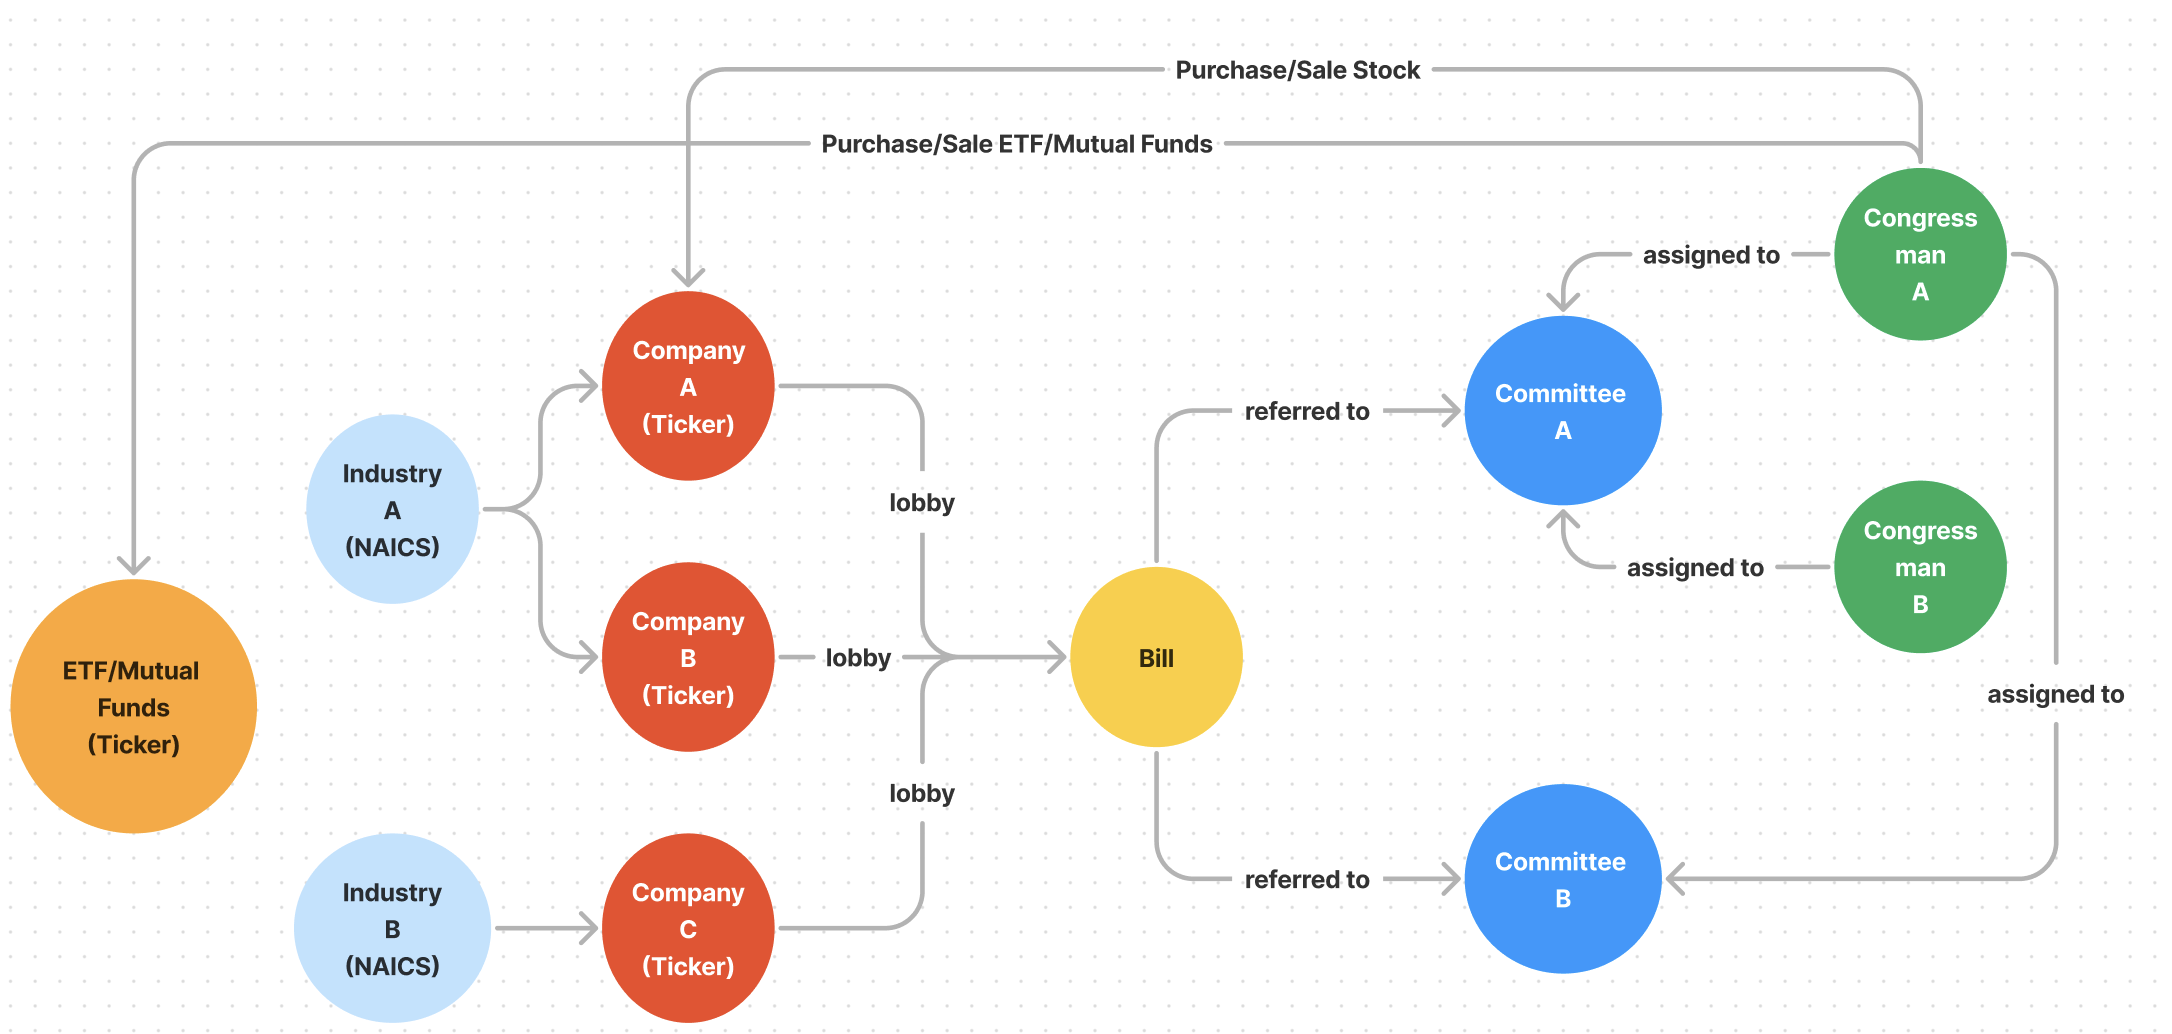
\includegraphics[width=1.0\textwidth]{imgs/etfmf.png}
  \caption{The network data includes various types of nodes and edges that represent different entities and interactions within the congressional activities and investment behavior of Congresspersons.}
  \label{fig:cbd}
\end{figure}

To provide a more concrete understanding of the data, Figure \ref{fig:trip} displays a subgraph related to Senator Ron Wyden's transaction in Trip Advisor stock (Ticker: TRIP). 
This subgraph illustrates the relationships between Senator Ron Wyden's congressional activities, including his membership in the Senate Finance Committee, his involvement with a specific bill related to airport improvements, and the economic sectors represented by NAICS codes, thereby providing insights into how these activities could potentially influence or be influenced by his stock transactions.

\begin{figure}[h]
  \centering
  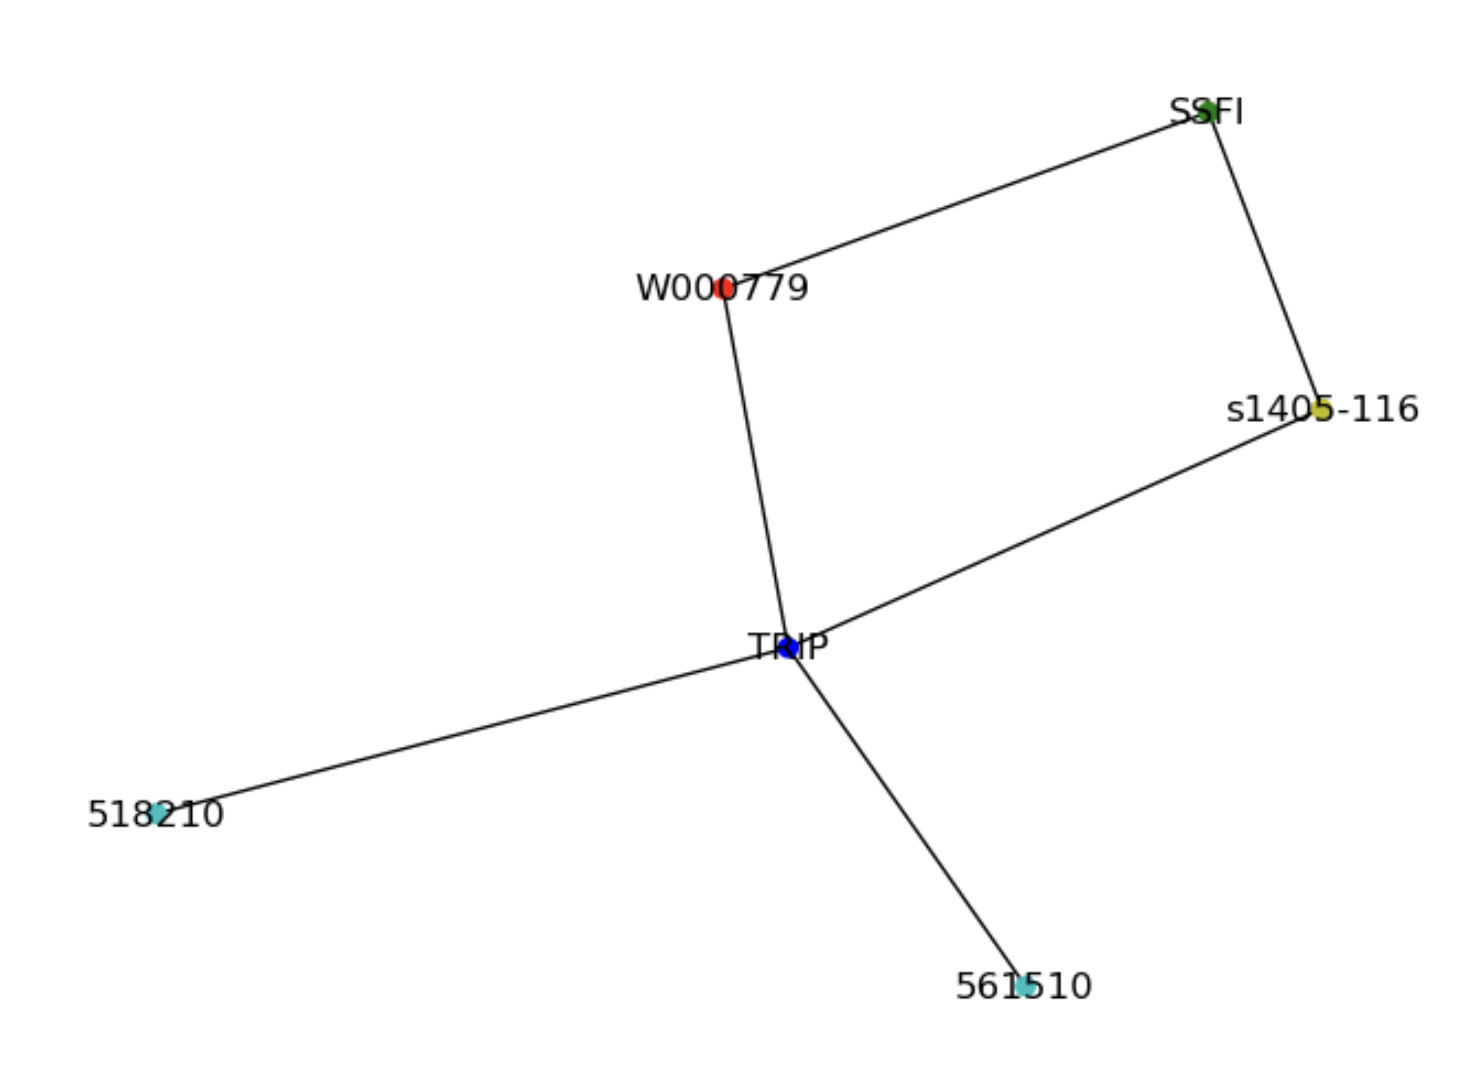
\includegraphics[width=1\textwidth]{imgs/trip.png}
  \caption{\textbf{A subgraph illustrating the congressional network related to the transaction of Senator Ron Wyden's Trip Advisor stock.} The node labeled W000779 corresponds to Ron Wyden's bioguide-id, which is a unique identifier provided by Congress for each senator. SSFI represents the Senate Finance Committee, of which Ron Wyden is a member. S1405-116 is a bill in the 116th Congress that revises requirements for the airport improvement program and pilot program for passenger facility charges at nonhub airports. The node labeled 518210 represents the NAICS Code for Data Processing, Hosting, and Related Services, while 561510 represents Travel Agencies.}
  \label{fig:trip}
\end{figure}

% In addition to the subgraph related to Senator Wyden's transactions, I also provide two more subgraphs in Figure \ref{fig:semi} and Figure \ref{fig:ssbk} to further aid understanding. These figures capture the industry-level congressional activities, illustrating how firms project their interests through lobbying to specific bills, and how committees oversee such bills. These subgraphs collectively demonstrate how firm/industry-level specific interests are funneled through lobbying to bills and aggregated to specific committees, ultimately conveying this information to congresspersons assigned to those committees. By examining these interconnections, we can gain a deeper understanding of the potential influences on stock transactions made by members of Congress.

% \begin{figure}[h!]
%   \centering
%   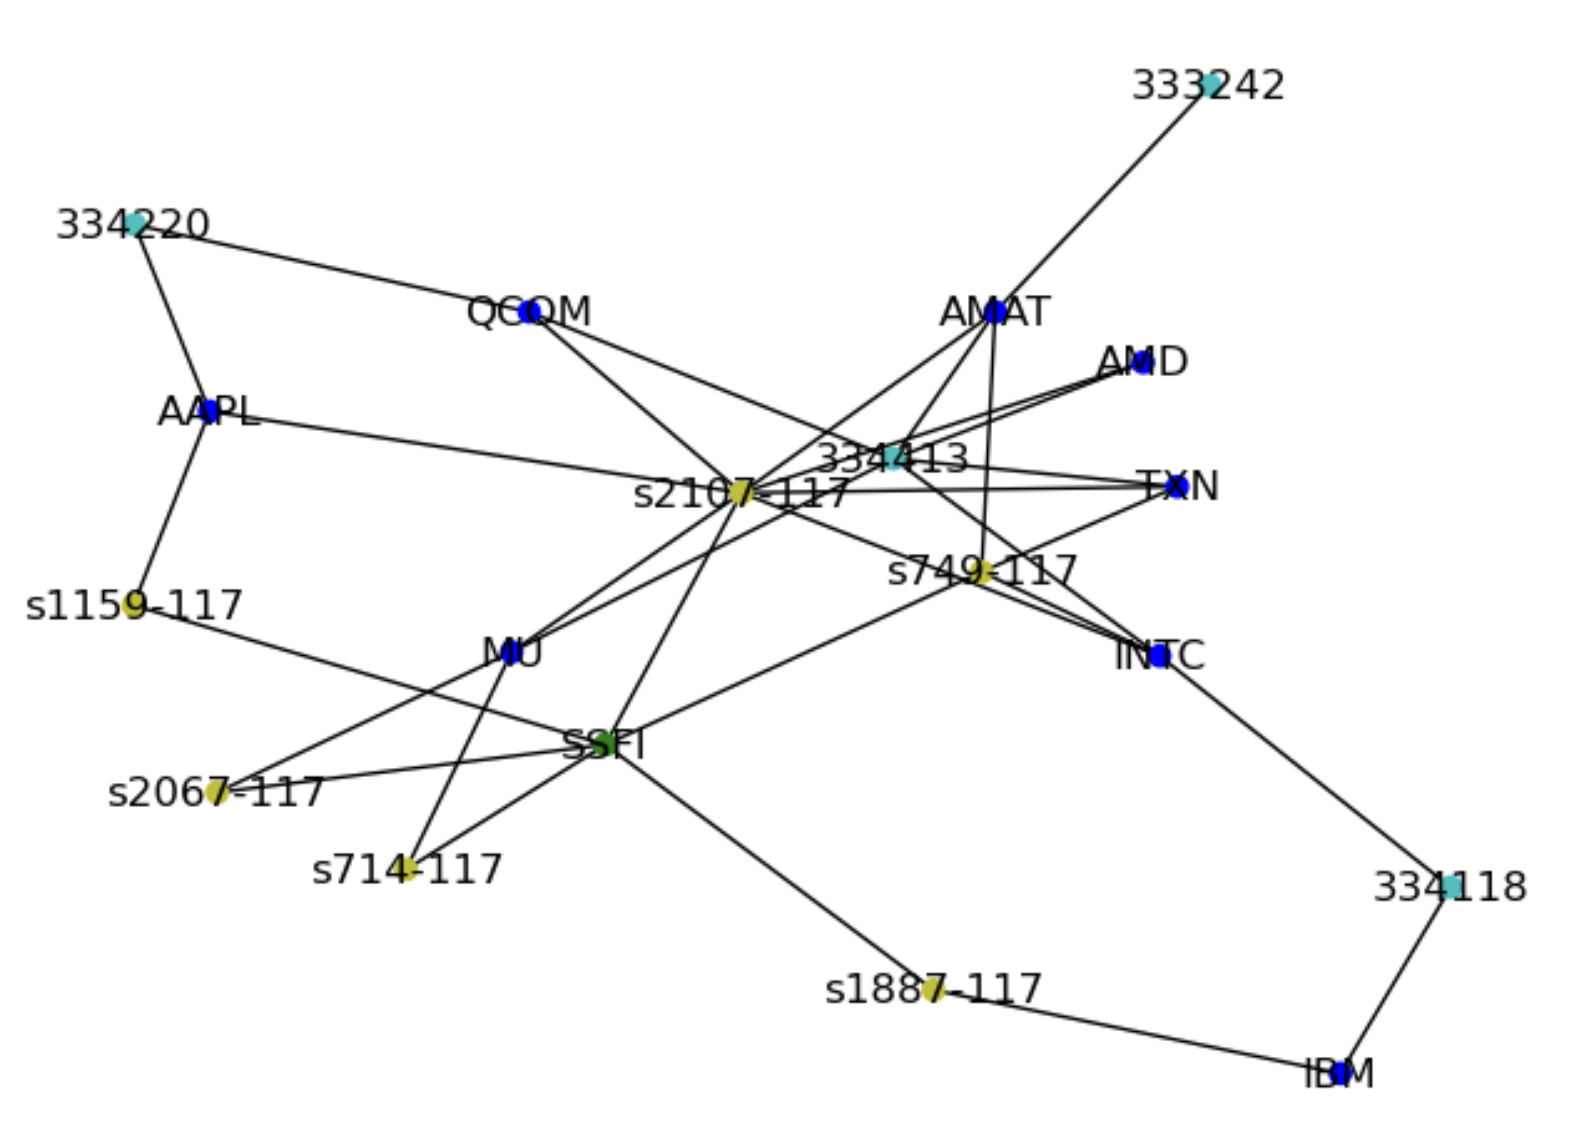
\includegraphics[width=1\textwidth]{imgs/semic.png}
%   \caption{\textbf{Subgraph capturing how the semiconductor industry's interests were funneled through the Senate Finance Committee during the 117th Congress} The NAICS code 334413 indicates Semiconductor and Related Device Manufacturing, which involves companies such as Qualcomm (QCOM), Intel (INTC), and Advanced Micro Devices (AMD), lobbying for bills such as S.2107 FABS Act and S.749 American Innovation and Jobs Act that are closely related to the subsidization of semiconductor manufacturing facilities. Relevant companies such as Apple Inc. and IBM, with NAICS codes of 334220 Wireless Communications Equipment Manufacturing and 334118 Computer Equipment Manufacturing, respectively, are direct customers of these semiconductor chips for manufacturing smartphone and computer hardware. The bills in which these companies have an interest are assigned to the Senate Finance Committee as well.
%   }
%   \label{fig:semi}
% \end{figure}

% \begin{figure}[h!]
%   \centering
%   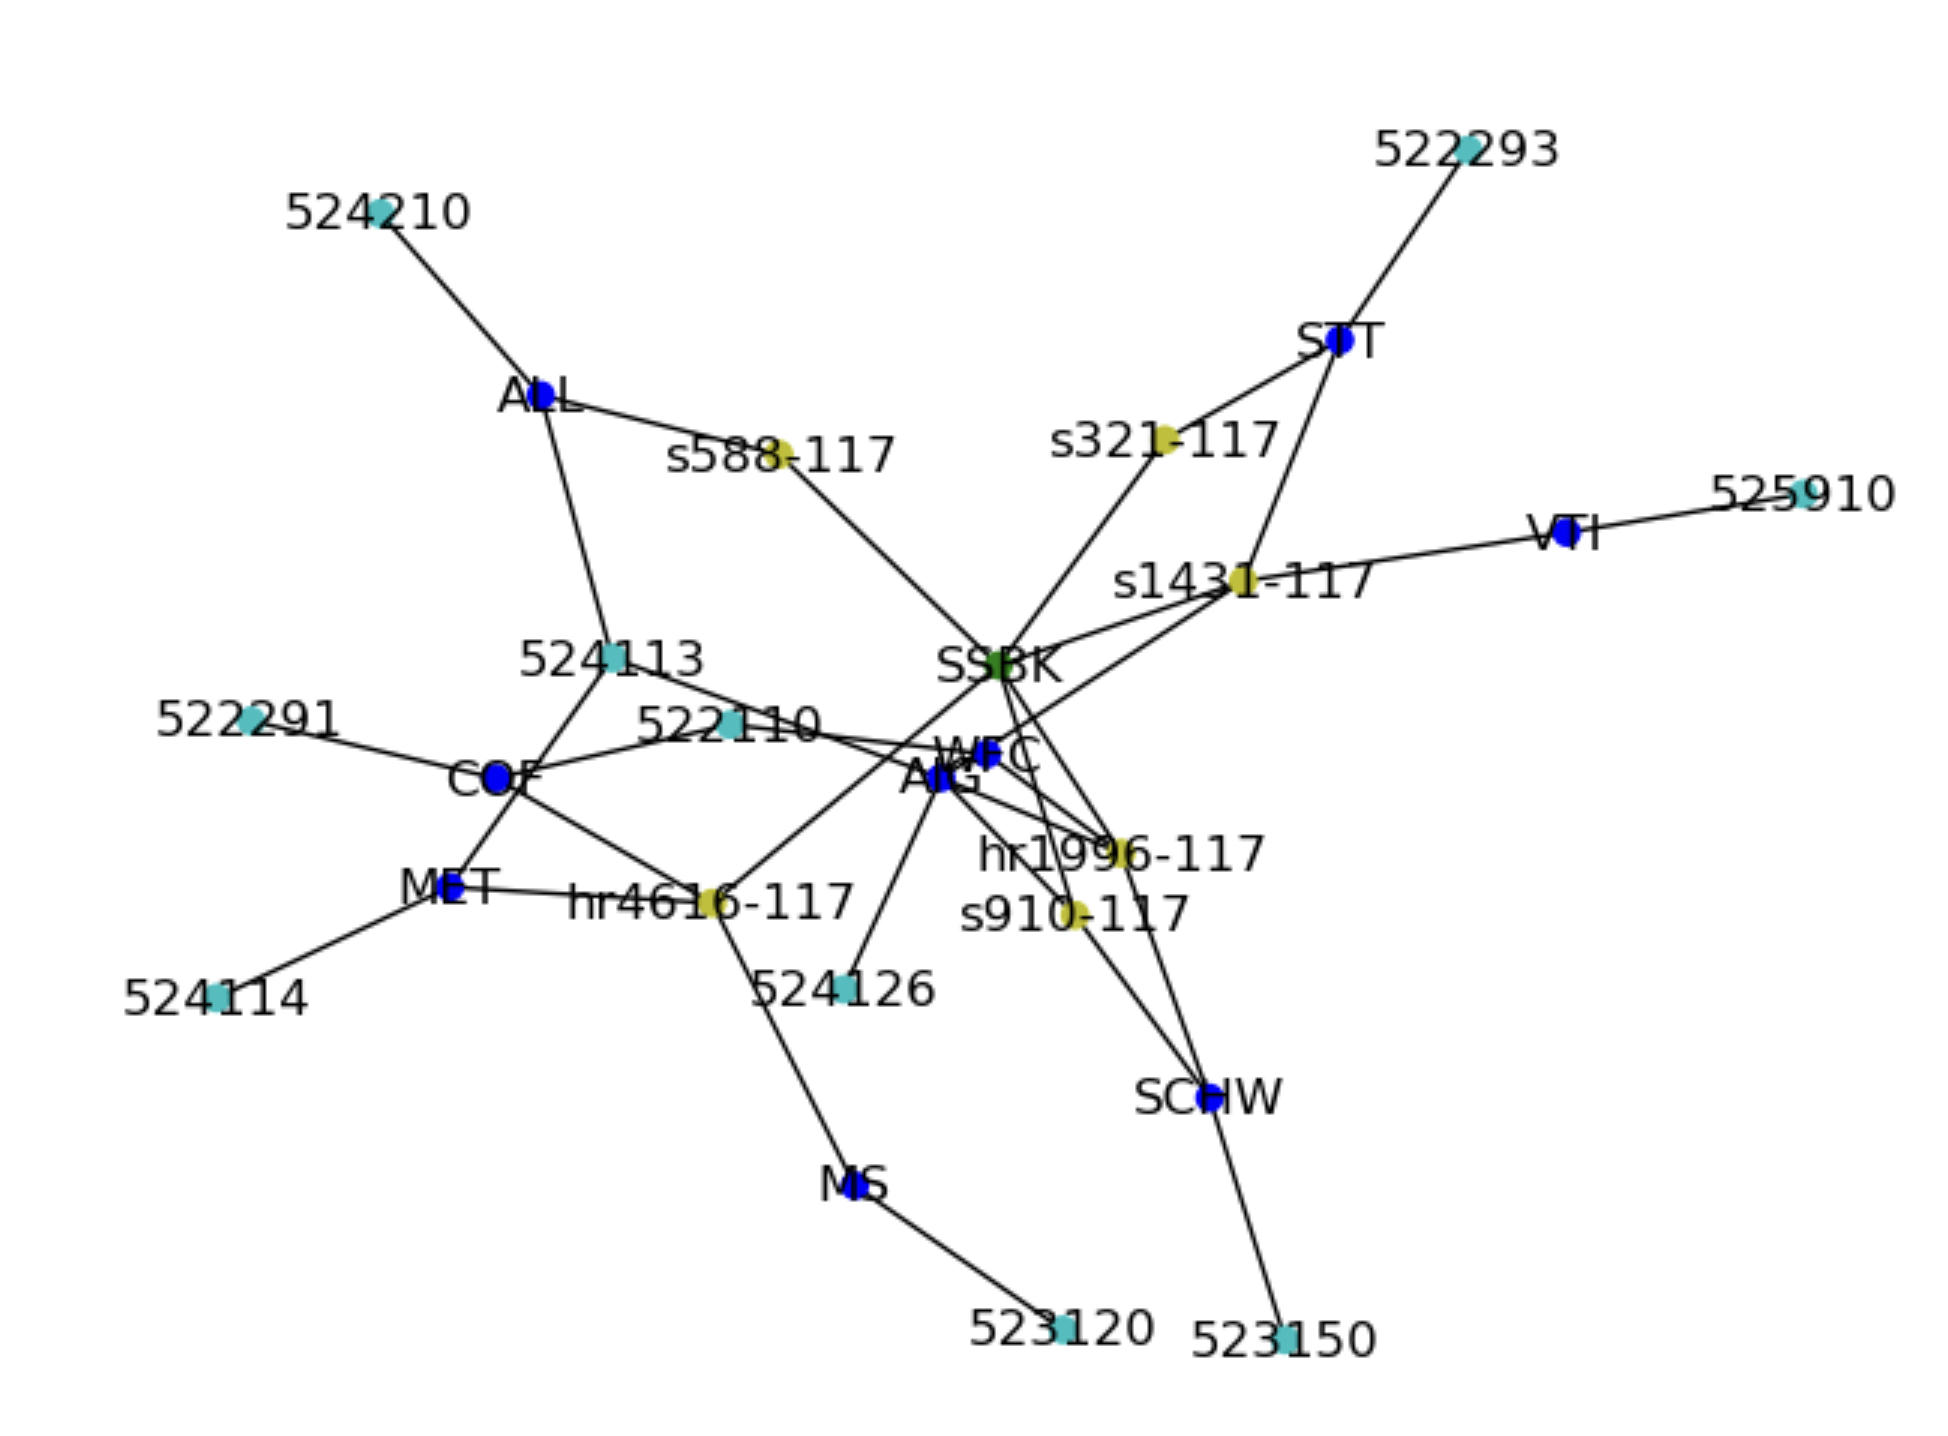
\includegraphics[width=1\textwidth]{imgs/SSBKs.png}
%   \caption{\textbf{Subgraph capturing how the financial industry's interests were funneled through the Senate Banking Committee during the 117th Congress} the Senate Banking Committee (SSBK) serves as a channel for different financial companies to project their lobbying interests over bills. NAICS codes starting from 52 generally relate to the financial industry in Figure \ref{fig:ssbk}. For instance, Wells Fargo (WFC) and AIG are lobbying for H.R.1996 - SAFE Banking Act of 2021, which prohibits a federal banking regulator from penalizing a depository institution for providing banking services to a legitimate cannabis-related business. Capital One Inc. (COF) and MetLife Inc. (MET) are lobbying for H.R.4616, which allows for the transition of certain financial contracts away from the London Interbank Offered Rate (LIBOR). These bills are all funneled through the Senate Banking Committee, thus a committee member of SSBK is more likely to be equipped with in-depth knowledge of the financial industry.
%   }
%   \label{fig:ssbk}
% \end{figure}

\section{Identifying Informative Predictors in Congressional Stock Trading Using an LLM Agent}

This section delves into the design of a link prediction task aimed at identifying key features and information within network data that are informative for predicting congressional stock trading. 
I employ an emerging tool - a Large Language Model (LLM) agent - notable for its ability to reason and act autonomously. 
By tasking this LLM agent with performing link prediction tasks across various legislator-ticker pairs, I assess the likelihood of transactions based on available network data. 
This approach leverages the agent's advanced reasoning capabilities to analyze connections within the graph structured data explained in Section 3, providing insights into the dynamics of congressional stock trading behavior.
% I find that the LLM agent can be particularly beneficial in analyzing high-dimensional network data, utilizing its discretion to stack up its own understanding and reflections on which features are beneficial to perform such a link prediction task.

\subsection{High-Dimensional Complexity and Theorization in Network Data}

In this section, I justify the use of a Large Language Model (LLM) agent in our study. The primary motivation for employing an LLM agent is to identify important features that can explain congressional stock trading behaviors in an interpretable manner. This task becomes particularly challenging with high-dimensional data, a common characteristic of graph-structured data. Unlike traditional tabular data, graph-structured data often involves large adjacency matrices that are highly dimensional, scaling as \( N^2 \) with \( N \) being the number of nodes \citep{Ward2011NetworkAA}.
This high dimensionality poses distinct challenges in data analysis and theorization, particularly when analyzing networks that capture societal phenomena \citep{Tang2012FeatureSW, Thi2013FeaturesEF}. 

In political science, handling high-dimensional data for tabular datasets has primarily 
been addressed using two methods: tree-based models and LASSO.
Tree-based models, as discussed in \cite{Montgomery}, are effective for detecting nonlinearities and interactions 
in datasets with many covariates. 
LASSO, as exemplified in \cite{lasso2}, is particularly beneficial for reducing model complexity by systematically identifying the most relevant predictors. This characteristic makes LASSO an effective tool for simplifying analyses in various domains, especially where reducing predictor dimensionality is crucial for clear interpretation.
These models are valued for their flexibility and ability to uncover complex relationships within data. 

However, for network data in political science, 
there is a noticeable gap in the methodology. 
The field currently lacks a widely agreed-upon approach to manage the high dimensionality inherent in graph-structured data \citep{Lazer2011NetworksIP,Ward2011NetworkAA}. 
The challenge of managing high dimensionality in graph-structured data is further intensified when using heterographs as predictors. Heterographs, characterized by their diverse node and edge types, offer a comprehensive data representation format for social phenomena. Despite this, they are infrequently employed in social network analysis. This underutilization is notable given their potential as a general framework for capturing the complexities of social interactions.

To address the challenges associated with the high dimensionality of graph-structured data, particularly when using heterographs as predictors in political science, this study introduces a novel method that leverages a Large Language Model (LLM) agent. The primary motivation behind employing an LLM agent is to effectively identify key features within the network—such as specific types of connections and combinations thereof—that can explain congressional stock trading behaviors in an interpretable manner.

The LLM agent's role in this context is to sift through the complex network data, pinpointing potential predictors that might otherwise be overlooked due to the data's high dimensionality. For example, it could be hypothesized that if a legislator assigned to a committee handles a significant number of bills targeted at a particular industry, this could be a strong predictor of whether that legislator engages in transactions of certain stock tickers related to the same industry.
The following sections will delve into a comprehensive explanation of what Large Language Models (LLMs) and LLM agents are, and the specific design of the theorizing agent being proposed.

\subsection{Large Language Models (LLMs) and LLM Agents}

Large Language Models (LLMs) are advanced AI systems capable of understanding, generating, and engaging with human language  \citep{Zhao2023ASO}. 
These models are trained on vast amounts of text data, allowing them to grasp a wide array of language patterns, nuances, and contexts. LLMs like OpenAI's GPT-3.5 and GPT-4 exemplify this technology's pinnacle \citep{Radford2018ImprovingLU}, demonstrating near-human-like reasoning abilities. These models can make decisions based on a complex understanding of language, context, and, to some extent, the logic and knowledge embedded in their training data \citep{Lampinen2022CanLM}.

One key characteristic of LLMs is their ability to generate coherent and contextually relevant text, making them particularly useful for a range of applications, from content creation to data analysis. In the realm of predictive modeling, LLMs stand out for their ability to process and interpret complex data structures in a way that mimics human cognitive processes \citep{Kojima2022LargeLM, Hayashi2019LatentRL}. 
This capability makes them highly valuable in fields like political science \citep{Luitse2021TheGT}, where interpreting intricate relationships within data is crucial.

Continuing from the foundational understanding of Large Language Models (LLMs), a notable trend in their application is the shift from using them as mere one-time question-answering systems to leveraging them in a more dynamic and interconnected manner. Expanding on this concept, the proposed approach seeks to enhance the problem-solving capabilities of LLMs by enabling them to dissect complex problems into a sequence of interconnected steps. This methodology facilitates a more detailed and systematic exploration of solutions, where each step builds on the insights gained from the previous one. By breaking down problems in this manner, LLMs can provide a more nuanced and comprehensive understanding of each component of the problem, leading to a potentially more effective and holistic solution \citep{cot, yao2023tree}.

In addition to the aforementioned step-by-step approach, there is an emerging trend of augmenting Large Language Models (LLMs) with a variety of tools, thereby enhancing their problem-solving capabilities. These augmented LLMs, or  ``LLM Agents'', are empowered to utilize these tools based on their own discretion and reasoning, choosing the most appropriate tool for a specific situation \citep{yao2023react}. For instance, an LLM augmented with web search tool can effectively invoke this tool as a part of its problem-solving process whenever it deems necessary.
Since LLM Agents are designed with an awareness of their own data cut-off points, recognizing the limitations in their training data up to a certain point in time. This self-awareness enables them to identify situations where their existing knowledge base may be insufficient. In such scenarios, an LLM Agent can decide to refer to external sources of data, such as the web or apis, to acquire more current and accurate information \citep{Qin2023ToolLLMFL, patil2023gorilla}. 

Then, how can we leverage these LLM Agents for theorizing and explaining complex phenomena such as congressional stock trading by letting them traverse over graph-structured data? This question opens up a new realm of possibilities in the application of LLM Agents. In the following section, I will propose a novel architecture that merges traditional machine learning techniques with the capabilities of LLM Agents. This hybrid approach aims to empower LLM Agents to not only analyze and interpret intricate data structures like graphs but also to generate their own explanations and hypotheses.

\subsection{Advancements in Designing Self-Learning LLM Agents}\label{llm-agent-lit}

The academic community and industry have shown considerable interest 
in exploring new applications of Large Language Models (LLMs), 
encountering unique challenges along the way. 
One significant issue is that LLMs, due to their immense parameter size 
and often proprietary nature, are difficult to fine-tune. 
While OpenAI offers fine-tuning options for the last few layers of models like GPT-3.5 and GPT-4, with user-prepared supervised input-output pairs, this process incurs additional costs and complexities.

Consequently, the focus has shifted towards designing learning experiences 
for LLMs that do not require traditional weight updates or parameter adjustments. 
This approach, known as ``no-derivative learning'', 
has rapidly evolved into a significant field of study \citep{yang2023large, zhu2023ghost, wang2023voyager}. 
It involves crafting system architectures that enable LLMs or LLM Agents to learn and achieve specific goals without altering their underlying LLM model weights.

A prime example of this method is the ``LLM as optimizer'' (OPRO) concept \citep{yang2023large}, which proposes no-derivative learning by creating a meta-prompt that is iteratively updated. The achievement of the task is scored, and this scoring is also conducted by LLM. This method demonstrates that prompts can evolve through self-evaluation or self-reflection, effectively allowing the LLM to function as an optimizer. This approach has been successfully applied to solve linear regression problems, showcasing the LLM's ability to operate in an optimizer-like capacity.

Furthermore, from the perspective of optimizing actions, \cite{shinn2023reflexion} introduced a verbally reflecting agent that generates task feedbacks. These feedbacks are then maintained in an episodic memory buffer, aiding the agent in making better decisions in subsequent trials. This concept of self-evaluation or self-reflection, through designing a meta-prompt that allows the agent to assess its own performance and store these reflections for future reference, has become another cornerstone of no-derivative learning.

Additionally, the \cite{wang2023voyager} presented a novel approach where embeddings of these reflections are stored in a vector database. 
This enables the utilization of similarity searches over vector space, enhancing the agent's ability to recall and act upon past experiences effectively. For instance, \cite{wang2023voyager} taught LLM Agents to play Minecraft by storing environment information as embeddings with corresponding skills as key-value pairs. These environment-skill pairs are retrieved based on the current environment, allowing the LLM Agent to augment its reasoning process with previously effective skill sets.

\subsection{Predictive Theorization with Self-Learning LLM Agents}

% The complex heterograph dataset comprising 55K nodes and 264K edges, incorporating 5 different types of nodes and edges. This heterograph encapsulates congressional activities, potentially influencing the stock trading behavior of congresspersons. The primary question is whether these activities affect stock trading and if it's possible to theorize or hypothesize about these behaviors, despite the data's high dimensionality and dense interconnections, which differ significantly from traditional tabular formats.
To analyze the dataset in Section \ref{sec:data}, 
a complex heterograph with 55K nodes and 264K edges featuring 5 distinct types of nodes and edges, 
we face a substantial challenge. This dataset, encapsulating a variety of congressional activities, 
offers insights into how these activities might influence the stock trading behavior of congresspersons. 
The central inquiry revolves around the impact of these activities on stock trading, aiming to develop theories or hypotheses about such behaviors. This endeavor is complicated by the dataset's high dimensionality and the dense interconnections of its heterograph structure, which markedly deviates from the simplicity of traditional tabular data formats.

As discussed in Section \ref{llm-agent-lit}, self-learning Large Language Model (LLM) Agents emerge as a promising solution to this challenge. By engaging these agents in iterative predictive tasks focused on the existence of links between legislator-ticker pairs, they can self-evaluate their performance. This process involves the agent assessing which observations within the dense graph data and which specific aspects of its topology or structure were pivotal in their problem-solving approach.

In this context, I propose an innovative methodology where the traditional task of link prediction is approached through a self-learning LLM Agent. This method entails having the Agent predict the presence or absence of a link for a given legislator-ticker pair. Following each prediction, the agent engages in self-reflection or evaluation, analyzing the reasons behind its success or failure in comparison to the ground truth.

This approach not only leverages the advanced capabilities of LLMs in handling high-dimensional data but also introduces a novel dimension of self-assessment and learning. It allows the LLM Agent to progressively refine its understanding and approach to the data, potentially uncovering significant insights about the relationship between congressional activities and stock trading behaviors. 

In the subsequent subsection, 
I will delve into the detailed design of this agent, elaborating on the specific tasks it was assigned and the methodology employed in its development. 
This will include a thorough explanation of how the agent operates, 
the nature of its self-learning and self-evaluating mechanisms, and the 
rationale behind how the agent organizes its memory in a manner that 
aids in formulating appropriate theories or hypotheses, 
which in turn facilitates its achievement of high accuracy in the link prediction task.


\subsubsection{Dual-Tool for the LLM Agent: GraphDB and MemoryDB Access}

In order to undertake the link prediction task within the complex heterograph dataset, I developed an LLM Agent endowed with two distinctive tools: Graph Database (GraphDB) Access and Memory Database (MemoryDB) Access as follows: 

\textbf{GraphDB Access:} This tool allows the agent to directly interact with the heterograph data from Section \ref{sec:data} stored in a GraphDB. The agent has the freedom to connect to this database and execute queries based on its own logic and requirements. For instance, it can formulate a query like``MATCH (l:Legislator)-[:Buy\_Sell] $\rightarrow$ (t:Ticker)-[:BELONGS\_TO] $\rightarrow$ (n:NAICS) 
RETURN t.ticker", which could retrieve a list of all stock tickers that a legislator has transacted in, provided these tickers belong to the same NAICS code industry classification as the Ticker of interest. This tool empowers the agent with the ability to dynamically explore and analyze the relational data stored in the graph database.

\textbf{MemoryDB Access:} The second key component is the MemoryDB Access, which allows the agent to connect with a Vector Database. This database serves as a repository for the agent's historical analysis and decision-making processes. Following each iteration of the link prediction task, the agent is programmed to self-generate feedback on its performance. This introspective process is informed by the agent's own logs and reasoning paths used during prediction.

From this self-reflection, the agent develops key-value pairs that encapsulate specific conditions and corresponding actions. The intention behind this mechanism is to create a set of principles that are not only applicable to the current scenario but also generalizable to future tasks. These principles are then converted into text-based dictionary formats, each paired with an OpenAI embedding that represents the textual description of the conditions. These embeddings, along with their associated condition-action pairs, are stored in the Vector Database.

This approach enables the agent to query the Vector Database for relevant decision-making criteria when faced with similar conditions in the future where the similarity is measured by the cosine similairy. Importantly, this system is designed to abstract away from specific legislator-ticker details, instead focusing on broader principles and strategies. By doing so, the agent is not just recalling past decisions but is actively learning and adapting its approach for improved predictive performance in future link prediction tasks.

Through this dual-tool system, the agent is equipped not only to access and analyze complex network data but also to learn from its experiences, improving its predictive accuracy and developing a more nuanced understanding of the underlying patterns and relationships within the data.

\subsubsection{Operational Details of the LLM Agent's Prediction and Reflection Pipeline}

This section elucidates the operational mechanics of the algorithm outlined in Algorithm \ref{alg:llm}, which governs the LLM Agent's functionality in the context of the link prediction task. The pipeline leverages GraphDB and MemoryDB tools, enabling the agent to iteratively perform predictions, evaluations, and self-reflections.

\vspace{5mm} % Adjust the '5mm' to the desired space

\begin{algorithm}[H]
  \caption{LLM Agent Prediction and Reflection Pipeline}
  \label{alg:llm}
  \SetAlgoLined
  % \KwResult{Improved agent prediction and reflection capabilities}
  LLM $\leftarrow$ initialize LLM with model specification\;
  $graphDB, memoryDB \leftarrow$ initialize database connectors\;
  $agent \leftarrow$ initialize agent with (LLM, graphDB, memoryDB)\;
  
  \ForEach{$(legislator, ticker, label)$ in $TrainDataset$}{
      $(pred, log) \leftarrow$ make\_pred$(legislator, ticker, agent)$\;
      $eval \leftarrow$ evaluate$(pred, label)$\;
      $reflection \leftarrow$ generate\_reflection$(log, eval, agent)$\;
      insert\_memory$(reflection, memoryDB)$\;
  }
  \end{algorithm}

\vspace{5mm} % Adjust the '5mm' to the desired space

\textbf{1. LLM Initialization with GPT-4-1106-preview (GPT4-Turbo):} The agent utilizes the LLM model specified as `gpt-4-1106-preview', commercially known as GPT4-Turbo. This model is chosen for its superior token-length limit, 128K, allowing the agent to process the largest possible context length among currently available GPT models by OpenAI. This extensive context handling capability is crucial for analyzing complex, high-dimensional data.

\textbf{2. Prediction Process:} The `make\_pred' function is executed by the agent using a prediction template. This template explicitly defines the task of link prediction, instructing the agent to determine the existence or non-existence of a link. The agent is guided to utilize specific data and tools. The template is available at Appendix \ref{app:log}.

\textbf{3. Evaluation Function:} The `evaluate' function returns a binary outcome – 1 for a successful prediction (correct link existence) and 0 for an unsuccessful one (incorrect prediction).

\textbf{4. Generation of Reflections:} Post-evaluation, the agent generates reflections in the form of a list of dictionaries, each containing 'condition' and `action' keys with their respective values. These reflections encapsulate the agent's reasoning and decision-making process in each prediction instance.
The reflection is executed by the agent using a reflection prompt template. The template is available at Appendix \ref{app:log}.

\textbf{5. Memory Insertion:} The `insert\_memory' function processes each `condition' in the reflection list, creating OpenAI embeddings for them. These embeddings, along with their associated actions, are then stored in the MemoryDB. This process facilitates the agent’s future recall and application of learned strategies and decisions.

An illustrative example demonstrating a complete cycle of this pipeline, specifically for the case of Ron Wyden's interaction with Applied Materials (AMAT), is provided in the Appendix \ref{app:log}. This example offers a practical insight into how the agent navigates through a single iteration of the prediction and reflection process.

\subsubsection{Assessment of the LLM Agent's Predictive Performance on Selected Cases}

I tested LLM Agent's capabilities on a carefully chosen subset of cases involving legislator-ticker pairs, 
with a focus on assessing its ability to predict transactional relationships. 
Due to the expansive nature of the dataset, which includes about 24K transaction edges, 
a full-scale analysis was constrained by both time and cost. A more practical approach was adopted, where the analysis was conducted on 20 cases, 
striking a balance between existent and non-existent transactional edges. This sample selection not only addressed resource limitations — costing approximately \$31 in total, averaging to \$1.55 per inference 
— but also adhered to a feasible time frame, with the entire process taking around 30 minutes, 
translating to roughly 1.5 minutes per case.

The top 10 Legislator-Ticker 
pairs, characterized by their 
unusually high excess returns as depicted in Figure \ref{fig:erfin}, were chosen. 
To maintain diversity among the legislators and to simulate a realistic scenario, only one pair per unique legislator was included. Additionally, for each legislator, a ticker with which they had no prior transactions was randomly selected to create a hypothetical `negative' edge. 
This approach not only facilitated a balanced examination of both positive and negative aspects of the transactional relationships but also allowed for a more fair understanding of the agent's predictive accuracy.

The selected cases are systematically detailed in Table \ref{tab:prediction_analysis}, 
providing an overview of the pairs analyzed and their respective classifications in terms of transaction existence. 
Following the detailed presentation of cases in Table \ref{tab:prediction_analysis}, the performance of the LLM Agent's predictions can be further elucidated by referencing the computed metrics, as outlined in Table \ref{tab:metrics}. 
This table presents the counts of True Positives (TP), True Negatives (TN), False Positives (FP), and False Negatives (FN), along with the calculated values for key performance indicators: Accuracy, Precision, Recall, and F1 Score.
% Overall, these metrics highlight the agent's strengths and weaknesses in its current predictive model. The moderate accuracy and balanced F1 Score suggest a fair level of performance, while the precision and recall indicate specific areas where further refinement and improvement could be beneficial. The insights gleaned from these metrics are crucial for guiding future enhancements to the agent’s predictive algorithms.

% This structured analysis offers valuable insights into the agent's performance in a controlled environment, highlighting its potential in navigating complex datasets while being mindful of practical constraints such as time and cost efficiency.

\begin{table}[h]
  \centering
  \caption{\textbf{Predictions on Legislator-Ticker Pairs using LLM Agent}}
  \begin{tabular}{|l|l|l|c|c|c|}
  \hline
  \textbf{Legislator} & \textbf{Ticker} & \textbf{Ticker Name} & \textbf{Pred} & \textbf{Label} & \textbf{Eval} \\
  \hline
  Ron Wyden & AMAT & Applied Materials & EXIST & EXIST & Accurate \\
  Ron Wyden & BKNG & Booking Holdings & EXIST & NON-EXIST & Inaccurate \\
  Angus King & QQQ & NASDAQ-100 & EXIST & EXIST & Accurate \\
  Angus King & CZR & Caesars Entertainment Inc & NON-EXIST & NON-EXIST & Accurate \\
  Sheldon Whitehouse & IHI & iShares US Medical Devices ETF & EXIST & EXIST & Accurate \\
  Sheldon Whitehouse & AVGO & Broadcom Inc. & NON-EXIST & NON-EXIST & Accurate \\
  Timothy Kaine & VB & Vanguard Small-Cap Index Fund & NON-EXIST & EXIST & Inaccurate \\
  Timothy Kaine & IJH & iShares Core S\&P Mid-Cap ETF & EXIST & NON-EXIST & Inaccurate \\
  David Perdue & DISCA & Warner Bros Discovery Inc & NON-EXIST & EXIST & Inaccurate \\
  David Perdue & XBI & SPDR S\&P Biotech ETF & EXIST & NON-EXIST & Inaccurate \\
  Mike Rounds & VCR & Vanguard Consumer Discretionary ETF & EXIST & EXIST & Accurate \\
  Mike Rounds & GLW & Corning Incorporated & EXIST & NON-EXIST & Inaccurate \\
  Jerry Moran & FB & Facebook & NON-EXIST & EXIST & Inaccurate \\
  Jerry Moran & RF & Regions Financial Corp & EXIST & NON-EXIST & Inaccurate \\
  Benjamin Cardin & XLC & Communication Services Select Sector & EXIST & EXIST & Accurate \\
  Benjamin Cardin & WMT & Walmart & EXIST & NON-EXIST & Inaccurate \\
  Shelley Capito & MSFT & Microsoft Corporation & EXIST & EXIST & Accurate \\
  Shelley Capito & SNE & Snap-On Inc & NON-EXIST & NON-EXIST & Accurate \\
  Pat Roberts & WMT & Walmart & EXIST & EXIST & Accurate \\
  Pat Roberts & CB & Chubb Limited & NON-EXIST & NON-EXIST & Accurate \\
  \hline
  \end{tabular}
  \label{tab:prediction_analysis}
  \end{table}

  \begin{table}[h]
    \centering
    \caption{\textbf{Performance Metrics of the LLM Agent's Predictions}}
    \begin{tabular}{|l|c|}
    \hline
    \textbf{Metric} & \textbf{Value} \\
    \hline
    True Positives (TP) & 7 \\
    True Negatives (TN) & 4 \\
    False Positives (FP) & 6 \\
    False Negatives (FN) & 3 \\
    \hline
    Accuracy & $\frac{TP + TN}{TP + TN + FP + FN} = \frac{7 + 4}{7 + 4 + 6 + 3} = 0.55$ \\
    Precision & $\frac{TP}{TP + FP} = \frac{7}{7 + 6} = 0.5385$ \\
    Recall & $\frac{TP}{TP + FN} = \frac{7}{7 + 3} = 0.7$ \\
    F1 Score & $2 \cdot \frac{\text{Precision} \times \text{Recall}}{\text{Precision} + \text{Recall}} = 2 \cdot \frac{0.5385 \times 0.7}{0.5385 + 0.7} = 0.6087$ \\
    \hline
    \end{tabular}
    \label{tab:metrics}
    \end{table}
  
The performance metrics of the LLM Agent, as detailed in Table \ref{tab:metrics}, clearly indicate that its current level of predictive accuracy and precision is suboptimal. 
The low accuracy and precision suggest that the agent is not yet sufficiently reliable, particularly due to its tendency to produce a significant number of false positives. 
This performance shortfall underscores the need for further refinement and training of the agent, especially considering the limited size of the dataset used for its evaluation.
It's important to recognize, however, that this outcome is largely influenced by the nature and scale of the dataset used for the learning task. The agent's training and evaluation were conducted on a relatively small set of data, comprising just 20 cases.

However, it is crucial to highlight the LLM Agent's innate ability to develop its own hypotheses and theorization through reflection. This capability is demonstrated by its continual generation of conditions, directing its focus on specific features by utilizing its memory module. This aspect of self-reflection and self-directed learning shows promise in the agent's development, indicating a capabilities of reasoning and adaptability. 
In the following subsection, I will delve deeper into the contents of the memory module, exploring and investigating the hypotheses and theories formulated by the agent during its learning process. This examination will shed light on the agent's internal reasoning mechanisms and its potential for growth and improved performance with further training and exposure to more extensive datasets.

\subsubsection{Exploration of the LLM Agent's Memory Module: Unraveling Internal Hypotheses and Theorizations}

During the training involving 20 distinct pairs of legislator and ticker data, the LLM Agent successfully generated and stored 27 unique condition-action pairs within its memory module. 
This accumulation of pairs indicates the agent's ability to recognize and adapt to a variety of scenarios. 
Below is one such example that illustrates how the agent operates:

\vspace{5mm} % Adjust the '5mm' to the desired space

\begin{mdframed}
\textbf{Example Condition-Action Pair:}

\textbf{Condition:} When a publicly traded company has lobbied on bills that are assigned to the committees a legislator is a member of.

\textbf{Action:} Investigate the bills lobbied by the ticker and their assignment to the legislator's committees using the following Cypher query: \texttt{`MATCH (t:Ticker)-[:LOBBY\_ON]->(b:Bill) MATCH (b)-[:ASSIGNED\_TO]->(c:Committee) WHERE c.id = `<committee\_id>' RETURN b.official\_title, b.id'}, and then predict 'EXIST' based on the relevance of the bills to the legislator's committee assignments.

\textbf{Interpretation of the Cypher Query:} This query extracts data from a graph database, focusing on the interaction between legislative committees and lobbying efforts by companies. Specifically, it identifies bills that a company (ticker) has lobbied for and which have been assigned to specific committees that a legislator is part of. By specifying a committee ID, the query returns the titles and IDs of relevant bills. This information is used to assess the potential influence of the company's lobbying efforts on the legislator, based on their committee involvement. 
If there's significant relevance found between the lobbying activities and the legislator's committee work, the agent predicts an `EXIST' relationship, suggesting a possible transactional or influential connection.
\end{mdframed}

\vspace{5mm} % Adjust the '5mm' to the desired space

Following the specific example provided above, for a broader understanding of the LLM Agent's learning and decision-making capabilities, GPT-4 was employed to summarize all 27 unique condition-action pairs. This synthesis allows for a convenient interpretation of the agent's internal hypotheses and theories, providing insights into its reasoning process:

\vspace{5mm} % Adjust the '5mm' to the desired space

\begin{mdframed}
  \subsection*{Consolidated Summary of Memory Pairs}
  % \textbf{Overview:} 
  % Over the course of training with 20 legislator-ticker pairs, the agent developed 27 unique memory entries. These entries, consolidated and categorized for clarity, represent the agent's learning and decision-making processes.
  
  \subsubsection*{Category: Legislative Committee and Ticker Lobbying Interactions}
  \textbf{Condition:} When a ticker (company) lobbies on bills related to a legislator's committee assignments.\\
  \textbf{Actions:} 
  \begin{itemize}
      \item Investigate lobbyist activities and committee assignments.
      \item Predict `EXIST' for a `BUY\_SELL' relationship based on bill-ticker-legislator committee overlaps.
  \end{itemize}
  \textbf{Cypher Query:} 
  \begin{verbatim}
  MATCH (t:Ticker)-[:LOBBY_ON]->(b:Bill)-[:ASSIGNED_TO]->(c:Committee),
        (l:Legislator)-[:COMMITTEE_ASSIGNMENT]->(c)
  WHERE t.ticker = '<Ticker>' RETURN b.official_title, b.id
  \end{verbatim}
  
  \subsubsection*{Category: ETF Sector and Legislative Committee Alignment}
  \textbf{Condition:} When an ETF's sector representation aligns with a legislator's committee memberships.
  \\ \textbf{Actions:}
  \begin{itemize}
      \item Predict `EXIST' for `BUY\_SELL' relationships considering sector overlap.
  \end{itemize}
  \textbf{Cypher Query:} 
  \begin{verbatim}
  MATCH (t:Ticker {ticker: '<ETF_Ticker>'})-[:BELONGS_TO]->(n:NAICS)
  RETURN n.desc
  \end{verbatim}
  
  \subsubsection*{Category: Broad Indirect Connections}
  \textbf{Condition:} Absence of direct `BUY\_SELL' relationship data and lack of explicit NAICS code overlaps.
  \\ \textbf{Actions:}
  \begin{itemize}
      \item Explore broader indirect connections like historical trading patterns, personal interests, or market trends.
  \end{itemize}
  
  \subsubsection*{Category: Industry-Specific Legislative Influence}
  \textbf{Condition:} Legislators with transactions in specific NAICS categories and companies lobbying on related bills.
  \\\textbf{Actions:}
  \begin{itemize}
      \item Investigate committee assignments relevant to the industry of a ticker.
      \item Predict `EXIST' based on industry interests and legislative influence.
  \end{itemize}
  \textbf{Cypher Query:} 
  \begin{verbatim}
  MATCH (l:Legislator)-[:COMMITTEE_ASSIGNMENT]->(c:Committee), 
        (t:Ticker)-[:LOBBY_ON]->(b:Bill)
  WHERE l.bioguide = '<bioguide>' AND t.ticker = '<Ticker>' 
  RETURN b.official_title, b.id
  \end{verbatim}
  
  \end{mdframed}

  \vspace{5mm} % Adjust the '5mm' to the desired space

  As evidenced in the above summary, the Agent demonstrates a capacity for generating decision-making frameworks autonomously. This process involves the identification of specific conditions under which relevant information is collected using Cypher queries, and subsequent decision-making based on these established conditions.
  
  This capability is not just a testament to the Agent's advanced analytical abilities but also opens up new possibilities in the realm of theory building. By allowing the LLM to stack memories and reflect upon them, researchers can derive nuanced insights and form hypotheses based on the model's internal decision-making patterns. This method showcases a novel way of leveraging Large Language Models for more than just data analysis, extending into the domain of theoretical development and hypothesis generation.
  
  Furthermore, the hypotheses formulated by the Agent lead us to an intriguing avenue for further exploration. The next phase of this study will focus on a detailed comparison between the industry codes of legislators' stock portfolios and those associated with their committee assignments. By examining these industry distributions and drawing on data from both the stock transactions and the committees' lobbying activities, the study aims to uncover any significant correlations that might suggest legislative influence in specific industry sectors. This comparison will be instrumental in understanding the extent to which committee assignments may affect or reflect congressional stock trading behaviors.
  
\vspace{5mm} % Adjust the '5mm' to the desired space

% The LLM Agent's memory module, containing 27 unique entries, demonstrates its capability to generate hypotheses and decide on actions under specific conditions. These entries, each a unique condition-action pair, can be broadly categorized and summarized to understand the agent's learning process. A decision tree-like structure would be an effective way to visualize this learning, although it's important to note that creating an actual decision tree from these entries would be complex and would require a detailed analysis of each condition and action. Below is a high-level summary of the agent's learning, organized in a decision tree-like format:

% Condition: Absence of Direct 'BUY_SELL' Relationship

% Action: Use indirect evidence like committee assignments and bill lobbying activities.
% Cypher Query: 'MATCH (l:Legislator {bioguide: '<bioguide>'})-[:COMMITTEE_ASSIGNMENT]->(c:Committee)<-[:ASSIGNED_TO]-(b:Bill)<-[:LOBBY_ON]-(t:Ticker {ticker: '<Ticker>'}) RETURN l.name, c.name, b.official_title, t.ticker'
% Condition: Broad Transactions Across Diverse Sectors

% Action: Predict 'EXIST' for 'BUY_SELL' relationships based on diverse interests.
% Cypher Query: None specific; general prediction based on behavioral patterns.
% Condition: Lobbying on Bills by Ticker Assigned to Legislator's Committees

% Action: Investigate the lobbyist activities and committee assignments.
% Cypher Query: 'MATCH (t:Ticker)-[:LOBBY_ON]->(b:Bill)-[:ASSIGNED_TO]->(c:Committee), (l:Legislator)-[:COMMITTEE_ASSIGNMENT]->(c) WHERE t.ticker = '<Ticker>' RETURN b.official_title, b.id'
% Condition: ETF's Sector Alignment with Legislator's Committees

% Action: Predict 'EXIST' based on sector overlap and committee memberships.
% Cypher Query: 'MATCH (t:Ticker {ticker: '<ETF_Ticker>'})-[:BELONGS_TO]->(n:NAICS) RETURN n.desc'
% Condition: Overlap in NAICS Sectors and No Direct 'BUY_SELL' Data

% Action: Predict 'EXIST' based on NAICS sector overlap.
% Cypher Query: None specific; prediction based on sector analysis.
% Condition: No Direct Evidence and No NAICS Code Overlaps

% Action: Consider broader indirect connections and historical trading patterns.
% Cypher Query: None specific; broader analysis beyond database entries.
% This summary provides an overview of the types of hypotheses and actions the LLM Agent has learned to generate. Each entry represents a unique scenario in which the agent determines the likelihood of a 'BUY_SELL' relationship, often employing Cypher queries to retrieve relevant data from the database. The agent shows an ability to adapt its strategies based on the available evidence, whether direct or indirect, and to utilize its memory module to guide its decision-making process in complex scenarios.






% In machine learning and particularly in tasks involving complex predictive modeling, the size and diversity of the training dataset play a crucial role in shaping the accuracy and generalizability of the model.
  
% A limited dataset may not provide a comprehensive representation of the varied and nuanced scenarios the model might encounter in a broader context. This restriction can lead to a model that is not thoroughly trained to handle diverse or rare occurrences, which in turn impacts its predictive accuracy and reliability.
  
% Therefore, while the current metrics provide valuable insights into the agent's present capabilities, they should be interpreted with an understanding of the constraints imposed by the limited training set. Expanding the dataset, introducing a wider range of scenarios, and incorporating more diverse data points could significantly enhance the agent's learning, leading to improvements in its predictive accuracy and overall utility.

% Network data, with its intricate web of relationships and interactions, requires more nuanced analytical tools that can effectively capture and analyze these dynamics. This gap underscores the need for innovative methods, like the LLM agent approach, which can navigate the complexities of network data and provide interpretable insights into phenomena such as congressional stock trading behaviors.










\section{Industry-level Similarities between Congresspersons and Committees}\label{sec:ce}

In this section\footnote{Reproducible code for this section is available at \url{https://github.com/syyunn/efd/blob/main/anlys/cycle/main9-transactions-desc-house-included.ipynb}}, I aim to examine the relationship between committee assignments and stock trading behavior among congress members, addressing the puzzle arising from \cite{eg14}'s findings. Despite their discovery of the role that political connections play in profitable transactions, they found no evidence that committee membership influenced investment decisions. This observation is strikingly contrary to the preponderance of literature highlighting the importance of committee assignments and the specialized knowledge they confer.

Numerous studies, such as \cite{patterson1970}, \cite{king1994}, and \cite{asher1974}, have focused on the role of committee assignments in shaping legislative outcomes, the impact of bill referral on committee specialization, and members' specialization in topics related to committees' jurisdiction, respectively. Further research reinforces this notion of committee assignments as platforms for leveraging congressperson's knowledge and expertise, as shown in \cite{10.2307/40709444, 10.2307/2111156, kiewiet1991logic, krehbiel1992information, curry2018knowledge}. The results of Egger and Hainmueller (2014) thus present a unique counterpoint, as they seem to contradict this prevailing understanding of committee roles in the legislative process.


Committee assignments provide congresspersons with unique access to information and resources related to specific industries and policy areas. As members of these committees, they are privy to the latest policy developments \citep{price1978policy}, market trends, and regulatory changes \citep{weiss1989congressional} that could potentially affect the performance of companies in the industries they oversee. The specialized knowledge and insights gained from participating in committee activities could inform their investment decisions and potentially influence their stock trading behavior. For example, they might be more inclined to invest in companies within their committee's jurisdiction due to their deeper understanding of the industry dynamics and future prospects. Furthermore, their committee roles could enable them to establish connections with industry stakeholders and gain access to non-public information that could potentially offer them an edge in making investment decisions.

% This section aims to provide more robust statistical evidence on the relationship between committee specialization and its potential implications on the stock trading behavior of Congress members by investigating the extent to which committee specialization resembles congresspeople's stock portfolio.
% I analyze the industry distributions of their stock transactions and committee assignments by computing the similarity between a committee's NAICS code distribution and that of the stocks transacted by the congressperson. 
% I compare the similarities between the congresspersons' stock transactions and the NAICS code distributions of committees they are assigned to against those they are not assigned to. 
This section aims to provide a more robust statistical examination of the correlation between committee specialization and the stock trading patterns of Congress members. Specifically, it probes the degree to which committee specialization mirrors the industry distribution of a Congress member's stock portfolio. This industry-focused analysis is justified by several observations and hypotheses:

1. As evidenced in Section \ref{sen-data}, approximately 60\% of the stock transactions by Senators involve ETFs or Mutual Funds. This indicates that congressional trading doesn't merely operate at the firm-level but extends to the industry-level, suggesting a possible connection between industry-specific knowledge and transaction behaviors.

2. On the data side, the graph-structured data introduced in Section \ref{sec:data} allows for the direct aggregation of industry-level committee specialization by tracing the link from firms lobbying on bills to the committees these bills are assigned to.

3. As shown in Figure \ref{fig:erfin}, many of the investments with high excess returns are industry-specific ETFs or Mutual funds. For instance, Senator Ron Wyden's collection of semiconductor stocks like AMAT, AVGO, and KLAC; Senator Mike Rounds' Financial Sector ETF; and Senator Sheldon Whitehouse's Medical Device ETFs. These observations underscore the need for an industry-level analysis that goes beyond firm-level stock trading.

In addition, the legal framework also favors an industry-level analysis. Following the STOCK Act 2012 and the corresponding Senate Ethics manual \citep{Boxer2012}, Congress members are prohibited from trading based on information obtained through their official duties. This suggests that leveraging not just firm-specific, but industry-level information garnered from congressional activities for trading is legally restricted. This study will hence scrutinize whether there exists a discernible pattern between committee specializations and industry-level stock transactions.

\subsection{Measuring Industry-level Specialization}

In this subsection, I will discuss the measurement of committee specialization in terms of industry-level specialization. By aggregating NAICS codes for the bills lobbied by various industries and those bills being referred to specific committees, I aim to quantify the industry-level specialization of each committee.

As an example, we can expect the Senate Banking Committee to have a higher degree of jurisdiction over banking-related issues, such as regulations tied to LIBOR (London Interbank Offered Rate) rates. This, in turn, would influence firms associated with NAICS codes related to banking (e.g., 52) to lobby the bills assigned to this committee more actively. This industry-level specialization can be effectively captured using the graph-structured data discussed in Section \ref{sec:data}. 
% Also, Figure \ref{fig:semi} and Figure \ref{fig:ssbk} from the previous section well illustrate industry-level specializations of Senate Fiinance and Banking committee for the semiconductor and banking industries, respectively.

To capture this industry-level specialization, I aggregate the North American Industry Classification System (NAICS) codes of each firm that is lobbying on each bill. These codes categorize each firm according to its primary business activity. I then look at the bills assigned to each committee. This allows to identify which industries - as represented by their NAICS codes - are most active in lobbying bills that fall under the purview of specific committees.
For instance, if a significant number of firms with the NAICS code for banking (52) are lobbying on bills assigned to the Senate Banking Committee, this would suggest a high degree of industry-level specialization of Senate Banking Committee on financial industry. This method of analysis, leveraging graph-structured data, allows us to explore the relationships between committee assignments, industries, and lobbying activities. 



To represent the committee-level specialization, I create a discrete probability distribution for each committee by aggregating the NAICS code distributions of firms that lobby bills assigned to those committees. Specifically, I count the occurrences of each NAICS code associated with firms that lobby bills referred to a particular committee. This method highlights the committee's industry focus, as it captures the concentration of lobbying efforts by firms within specific industries. Once we have the count-based frequency plot for each committee, we can easily convert it into a probability distribution function (PDF) by normalizing the counts with the total occurrences of all NAICS codes.

Similarly, to aggregate the NAICS code distribution of firms involved in each congressperson's stock transactions, we can simply count the occurrences of NAICS codes associated with all stock transactions executed by the congressperson (both purchases and sales). This provides a clear picture of the industries in which they invest, as the NAICS codes are derived from the firms whose stocks are being bought or sold by the congressperson in their stock transactions. We then normalize the count-based frequency plot with the total occurrences of all NAICS codes to obtain a PDF representing the congressperson's industry preferences.

% For both committee and congressperson, the aggregation of NAICS codes and the construction of discrete probability distributions based on the frequency of NAICS codes associated with lobbying activities and stock transactions provide insight into the industry preferences and focus areas.

As we've seen in Section \ref{excess}, the data used for estimating Senator's excess return shows that around 60\% of tickers are Exchange-Traded Funds (ETF)  or mutual funds, which are not single firms but representing certain industries or the stock market in general. For example, in Figure \ref{fig:erfin}, one of the highest excess returns, like the 45\% profit shown by Sen. Sheldon Whitehouse, is the ticker IHI, which is an ETF that invests in the US medical device market. Sen. Sheldon Whitehouse supported the Biden plan to fully utilize the Defense Production Act, increase the supply of necessary medical equipment and supplies\footnote{See \url{https://www.whitehouse.senate.gov/news/release/whitehouse-supports-biden-plan-to-fully-utilize-defense-production-act-increase-supply-of-necessary-medical-equipment-and-supplies}}. As shown, Senators do not always reflect their knowledge gained from congressional activities at the firm level but at the industry level. In either case, this measurement can effectively capture their level of specialization in certain industries in terms of their transaction patterns. By comparing the similarity between the two distributions, one from the committee and one from the congressperson, we can statistically test how similar they are to each other.

Subsequently, we measure the similarity between a congressperson's stock transactions' industry preference and a committee's industry specialization. This similarity can be quantified using cross entropy.
Cross-entropy is a useful statistical tool for determining the similarity between two distributions \citep{wu2018entropy, mao2013novel}, making it an ideal choice for comparing the distributions of NAICS codes for committee assignments and stock transactions. 
In this regard, for a given congressperson $i$ and committee $k$, the cross entropy $H_{ik}$ is computed as:

$$H_{i k}=-\sum_j P_{i, j} \log Q_{k, j}$$

Here, $P_{i,j}$ refers to the density of congressperson $i$'s trades in industry $j$ relative to all their transactions, and $Q_{k,j}$ denotes committee $k$'s specialization in industry $j$.

A lower cross entropy $H_{ik}$ suggests a higher similarity between the industry preference of congressperson $i$'s stock transactions and the industry specialization of committee $k$. This value is calculated at the congressperson-committee level, thereby providing an industry-level similarity measure between them.

Figure \ref{fig:density_plots} provides an example of this measurement for Sen. Sheldon Whitehouse's case. It displays the NAICS code distributions for Sen. Whitehouse's stock transactions, the Senate Finance Committee (SSFI), and the Senate Banking Committee (SSBK). The figure illustrates that the distribution of Sen. Whitehouse's stock transactions resembles the distribution of the Senate Finance Committee more closely than that of the Senate Banking Committee, highlighting the connection between his transactions and his committee assignments.

\begin{figure}[ht]
  \centering
  \begin{subfigure}[b]{0.3\textwidth}
      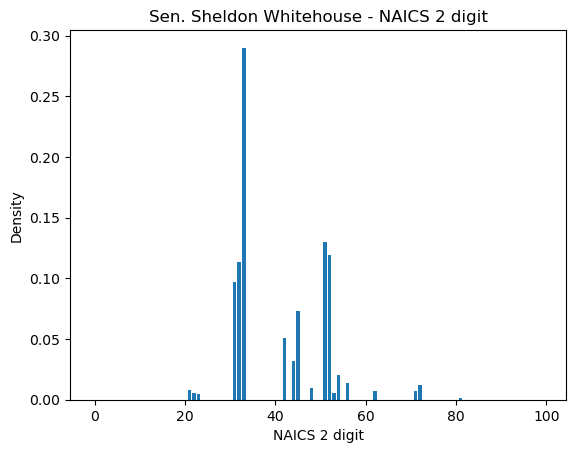
\includegraphics[width=\textwidth, height=0.2\textheight]{imgs/sheldonwhite.png}
      \caption{Sen. Sheldon Whitehouse's NAICS Distribution}
      \label{fig:senator_density}
  \end{subfigure}
  \hfill
  \begin{subfigure}[b]{0.3\textwidth}
      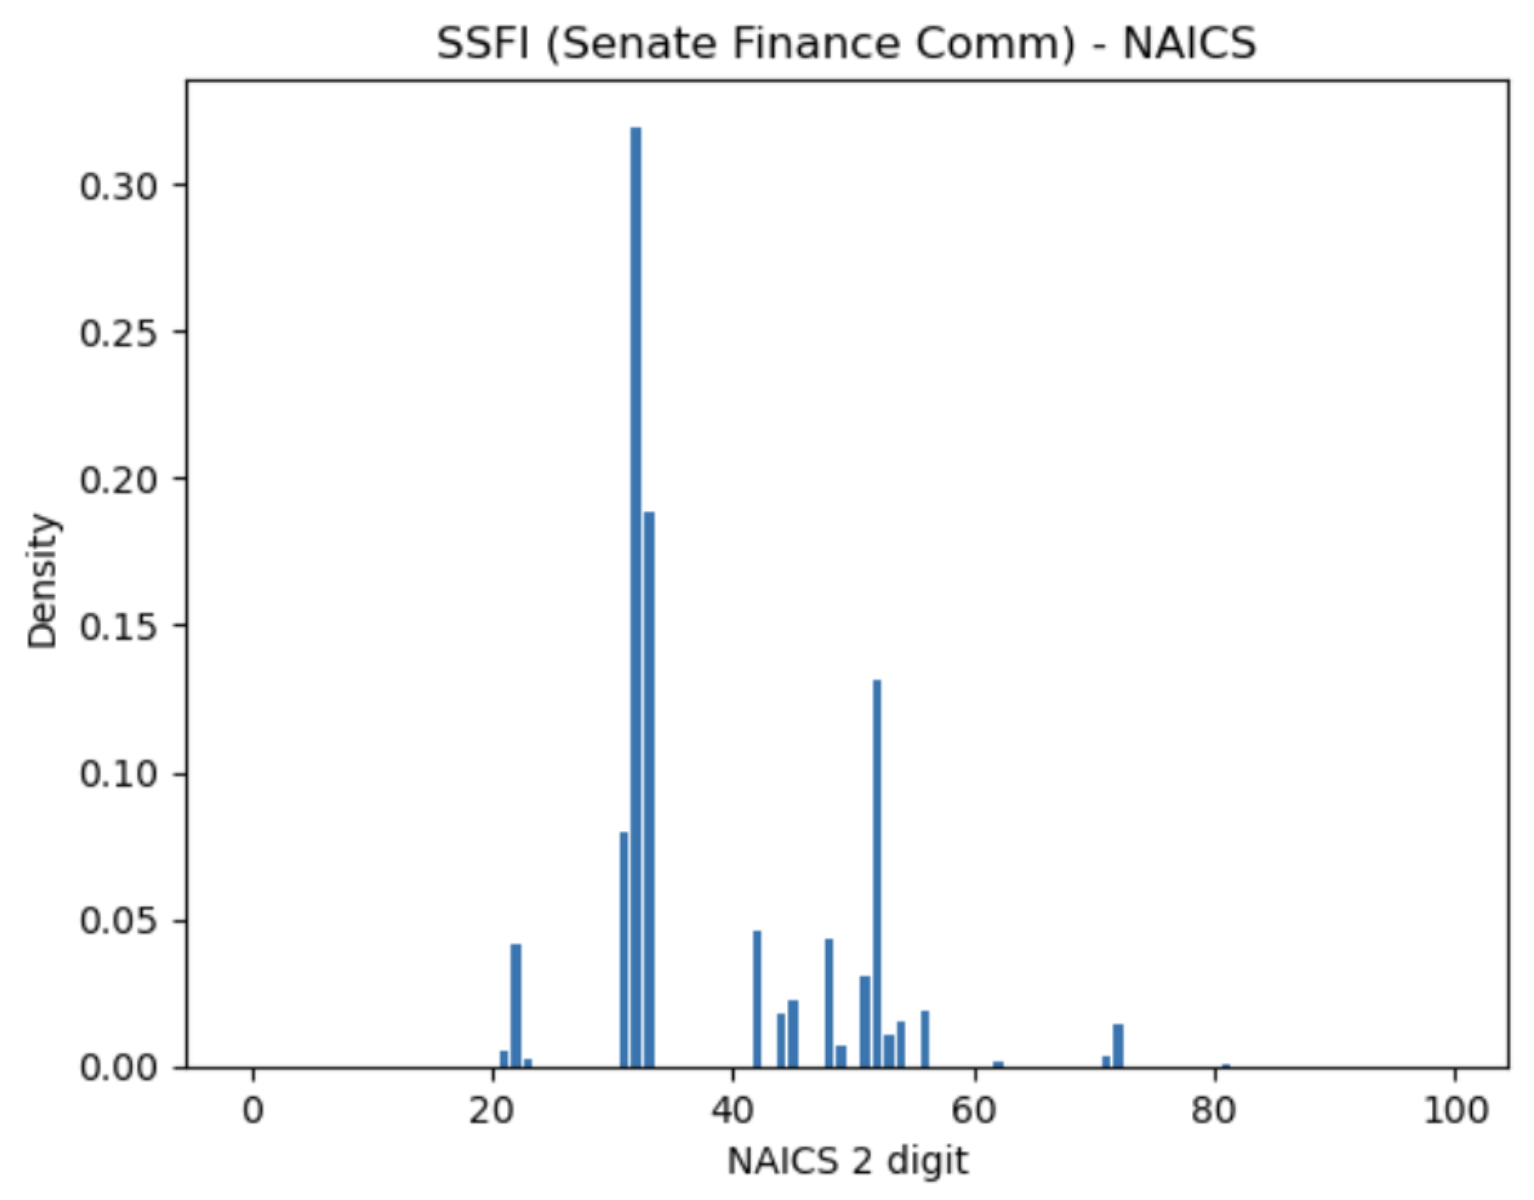
\includegraphics[width=\textwidth, height=0.2\textheight]{imgs/ssfi-entire2.png}
      \caption{Senate Finance Committee (SSFI) NAICS Distribution}
      \label{fig:ssfi_density}
  \end{subfigure}
  \hfill
  \begin{subfigure}[b]{0.3\textwidth}
      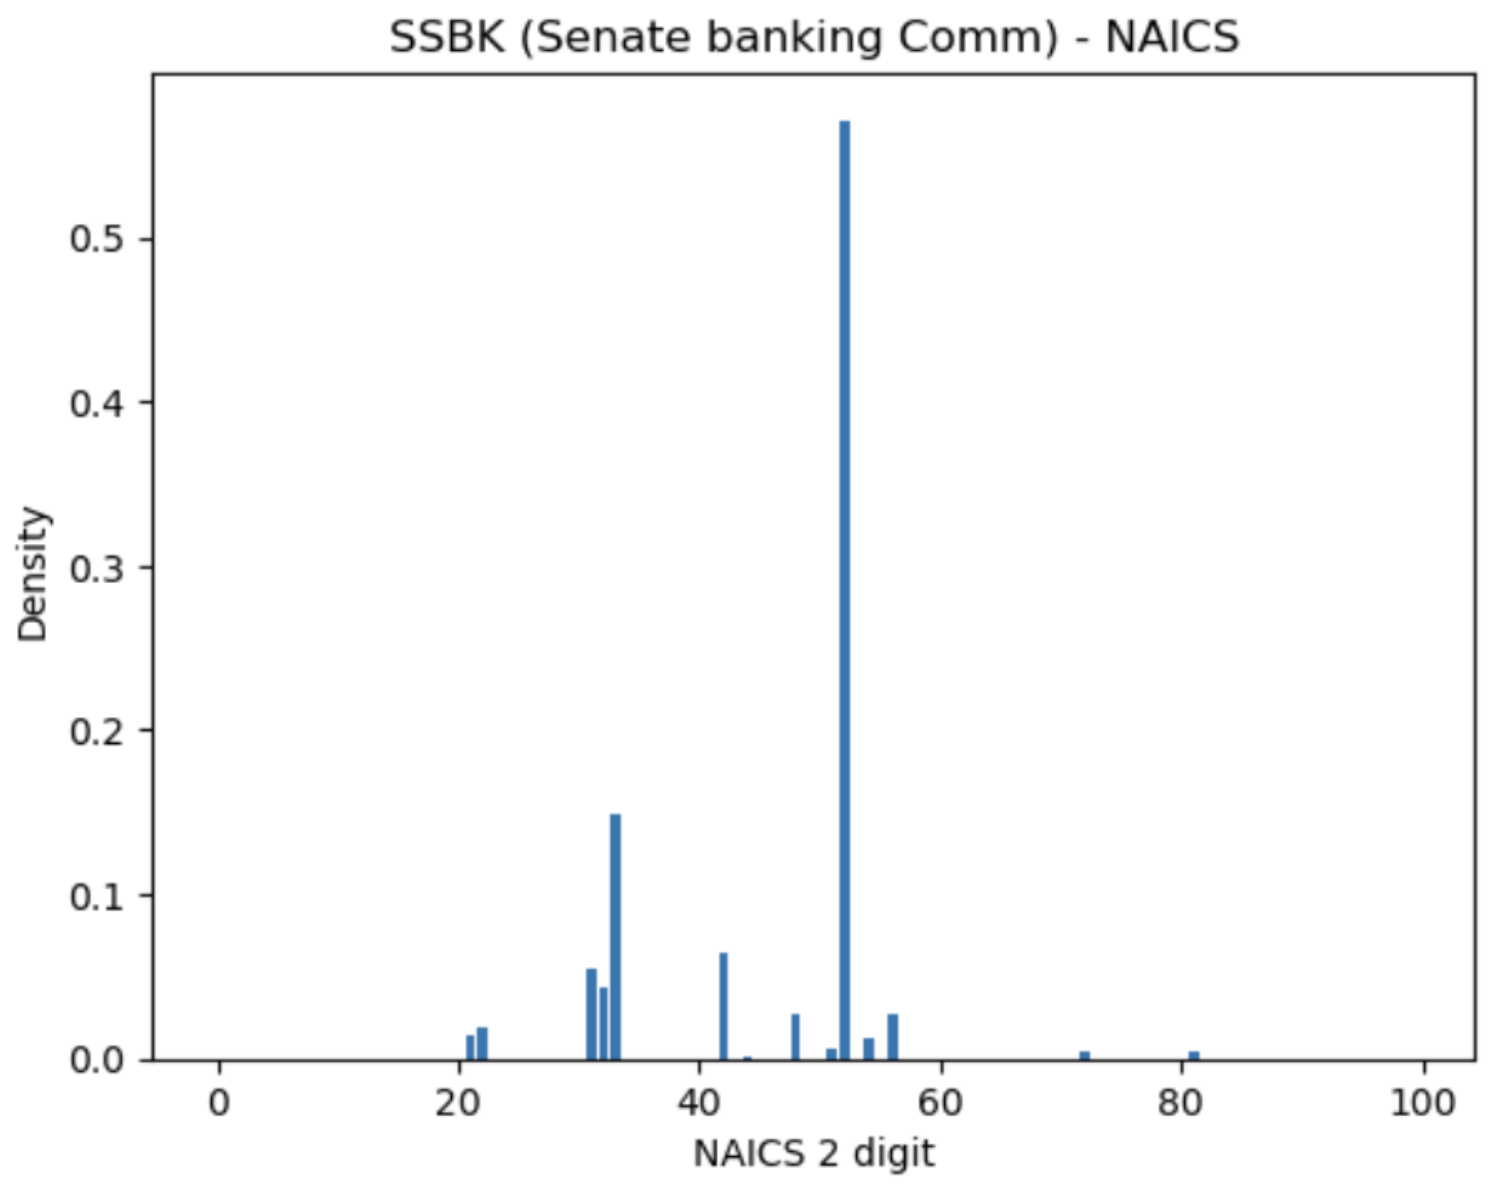
\includegraphics[width=\textwidth, height=0.2\textheight]{imgs/ssbk-entire2.png}
      \caption{Senate Banking Committee (SSBK) NAICS Distribution}
      \label{fig:ssbk_density}
  \end{subfigure}
  \caption{Comparison of NAICS code distributions for Sen. Sheldon Whitehouse, Senate Finance Committee (SSFI), and Senate Banking Committee (SSBK). The figure illustrates how the distribution of Sen. Whitehouse's stock transactions resembles the Senate Finance Committee's distribution more closely than that of the Senate Banking Committee.}
  \label{fig:density_plots}
\end{figure}

% To measure the similarity between the two discrete probability distributions, we can use cross-entropy. 
% Cross-entropy is a useful statistical tool for determining the similarity between two distributions \citep{wu2018entropy, mao2013novel}, making it an ideal choice for comparing the distributions of NAICS codes for committee assignments and stock transactions. 
In Figure \ref{fig:density_plots}, we can calculate the cross-entropy between Sen. Whitehouse's stock transaction distribution and the distributions of Senate Finance Committee (SSFI) and Senate Banking Committee (SSBK). The results are as follows:
\begin{align*}
  \text{Cross entropy (Sen. Sheldon Whitehouse, SSFI)} &= 0.816 \\
  \text{Cross entropy (Sen. Sheldon Whitehouse, SSBK)} &= 3.311
\end{align*}

These values indicate that Sen. Sheldon Whitehouse's investment portfolio is more similar to Senate Finance Committee in terms of NAICS code distribution, as a lower cross-entropy value represents a closer resemblance between the distributions.
This reflects that Sen. Whitehouse's stock portfolio more closely resembles the industry distribution of his own committee, the Senate Finance Committee (SSFI), compared to the Senate Banking Committee (SSBK), to which he does not belong.
Also, this suggests that the cross-entropy measure effectively captures the similarity between the industry-level specialization of a committee and the preferences reflected in a congressperson's stock portfolio. 

% This implies that a congressperson's committee assignments, and the specialized knowledge and focus areas associated with those committees, may indeed influence their stock transactions.






% \subsection{Evaluating the Impact of Committee Assignments on Stock Trading Behavior using Paired T-test}

% In this subsection, I perform a statistical test to determine whether there exists a significant difference in cross-entropy between two groups: assigned and unassigned committees.
% First, I computed the cross-entropy between the NAICS code distribution of stock transactions and committees, as explained in the previous section, for the 115th, 116th, and 117th Congresses. I also restricted the stock transaction dates to match each congressional term (e.g., for the 115th Congress, from January 2017 to January 2019) to ensure that only transactions during these periods were considered for the cross-entropy calculation.

% Senators and House Representatives are typically assigned to 4-5 committees for each congressional term. I computed the average cross-entropy for both assigned and unassigned committees. Then, I tested the significance of the mean cross-entropy values between the two groups using a paired t-test.
% Since it is reasonable to assume that the cross-entropy values within each pair are correlated, as committee assignments are based on a member’s relative specialization in various topics and industries, using a paired t-test is appropriate in this context. However, the assumption of independence between pairs might not be fully justified due to the dense connections between congress members and the potential for correlated behaviors.

% The results of the paired t-test can be found in Figure \ref{fig:paired_ttest}. The sample size is 235, which indicates that there are 235 unique pairs of (Congressperson, Congressional year). For example, one of the pairs includes Ron Wyden's average cross-entropy between the NAICS code distribution of his stock trading and assigned committees (Senate Finance, Budget, Intelligence, and Energy and Nuclear Resources Committee) and the remaining committees not assigned to him.

% \begin{figure}[h!]
% \centering
% 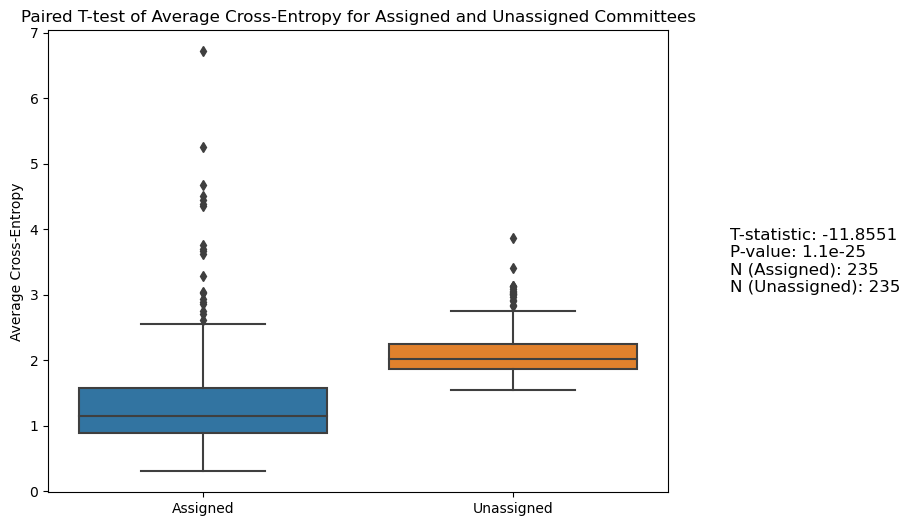
\includegraphics[width=1\textwidth]{imgs/paired.png}
% \caption{\textbf{Paired t-test results for the cross-entropy of assigned and unassigned committees.} The figure shows the comparison between the average cross-entropy of assigned and unassigned committees, with a sample size of 235 unique pairs of (Congressperson, Congressional year). The significantly lower average cross-entropy for the assigned group suggests that the stock trading patterns of Congress members more closely resemble the industry distribution of their assigned committees compared to unassigned committees.}
% \label{fig:paired_ttest}
% \end{figure}

% Despite the limitations of using a paired t-test, the results indicate that the average cross-entropy for the assigned group is significantly lower than that of the unassigned group. This suggests that the stock trading patterns of Congress members more closely resemble the industry distribution of their assigned committees compared to unassigned committees.

% Another potential limitation of this analysis is the difficulty in collecting NAICS codes for ETFs and Mutual Funds, which comprise approximately 60\% of the stock transactions in our dataset. Although each ETF or Mutual Fund's website provides information about their holdings, it was challenging to establish a generalizable pattern across different providers to obtain the composition of stocks held by these funds. Consequently, this study focuses on individual stocks and their corresponding NAICS codes, which might not fully capture the reality of Congress members' investments. However, the findings still indicate that the individual stock trading behaviors of Congress members are significantly influenced by their assigned committees.

\subsection{Paired T-Test: Comparing Assigned and Unassigned Committees}

In this subsection, I investigate whether there is a significant difference in the similarity between the industry distributions of Congress members' stock transactions and the industry distributions of their assigned and unassigned committees. 
To conduct this analysis, I computed the cross-entropy between the NAICS code distribution of stock transactions and committees for the 115th, 116th, and 117th Congresses. I restricted the stock transaction dates to match each congressional term (e.g., for the 115th Congress, from January 2017 to January 2019) to ensure that only transactions during these periods were considered.

Senators and House Representatives are typically assigned to several committees during each congressional term. For each Congress member $i$, and for each congressional term $t$, I calculated the cross-entropy $H_{i, k}^t$ between their stock transactions and each committee $k$ (both assigned and unassigned). The objective is to ascertain whether the industry preferences in a Congress member's stock transactions align more closely with the industry specializations of their assigned committees than those of unassigned committees.
To summarize these measurements, I calculated the mean cross-entropy value for each Congress member $i$ across all their assigned committees (denoted as $\bar{H}_{i, \text{assigned}}^t$), and the mean cross-entropy value across all their unassigned committees (denoted as $\bar{H}_{i, \text{unassigned}}^t$) for each congressional term $t$. The means here are taken over all committees $k$ that each Congress member $i$ is assigned or not assigned to respectively, for each term $t$.

To test this, I performed a one-sided paired t-test on the differences in these mean cross-entropy values for each congress member $i$ and congressional year $t$. The null hypothesis for this test was that the mean cross-entropy of assigned committees is less than or equal to that of unassigned committees for each Congress member and Congressional year ($\bar{H}_{i, \text{assigned}}^t \ge \bar{H}_{i, \text{unassigned}}^t$). The alternative hypothesis was that the mean cross-entropy of assigned committees is greater than that of unassigned committees ($\bar{H}_{i, \text{assigned}}^t < \bar{H}_{i, \text{unassigned}}^t$). A rejection of the null hypothesis would thus provide evidence that congressional activities significantly influence stock transaction behavior, indicating that a Congress person's stock trading pattern significantly resembles the committee's industry-level specialization.

% The paired t-test \citep{hsu2014paired} is appropriate in this context because the cross-entropy values within each pair (assigned and unassigned committees) are expected to be correlated. This correlation arises because committee assignments are based on a member's relative specialization in various topics and industries. However, the assumption of independence between pairs may not be fully justified due to the dense connections between Congress members and the potential for correlated behaviors.

\begin{figure}[h!]
  \centering
  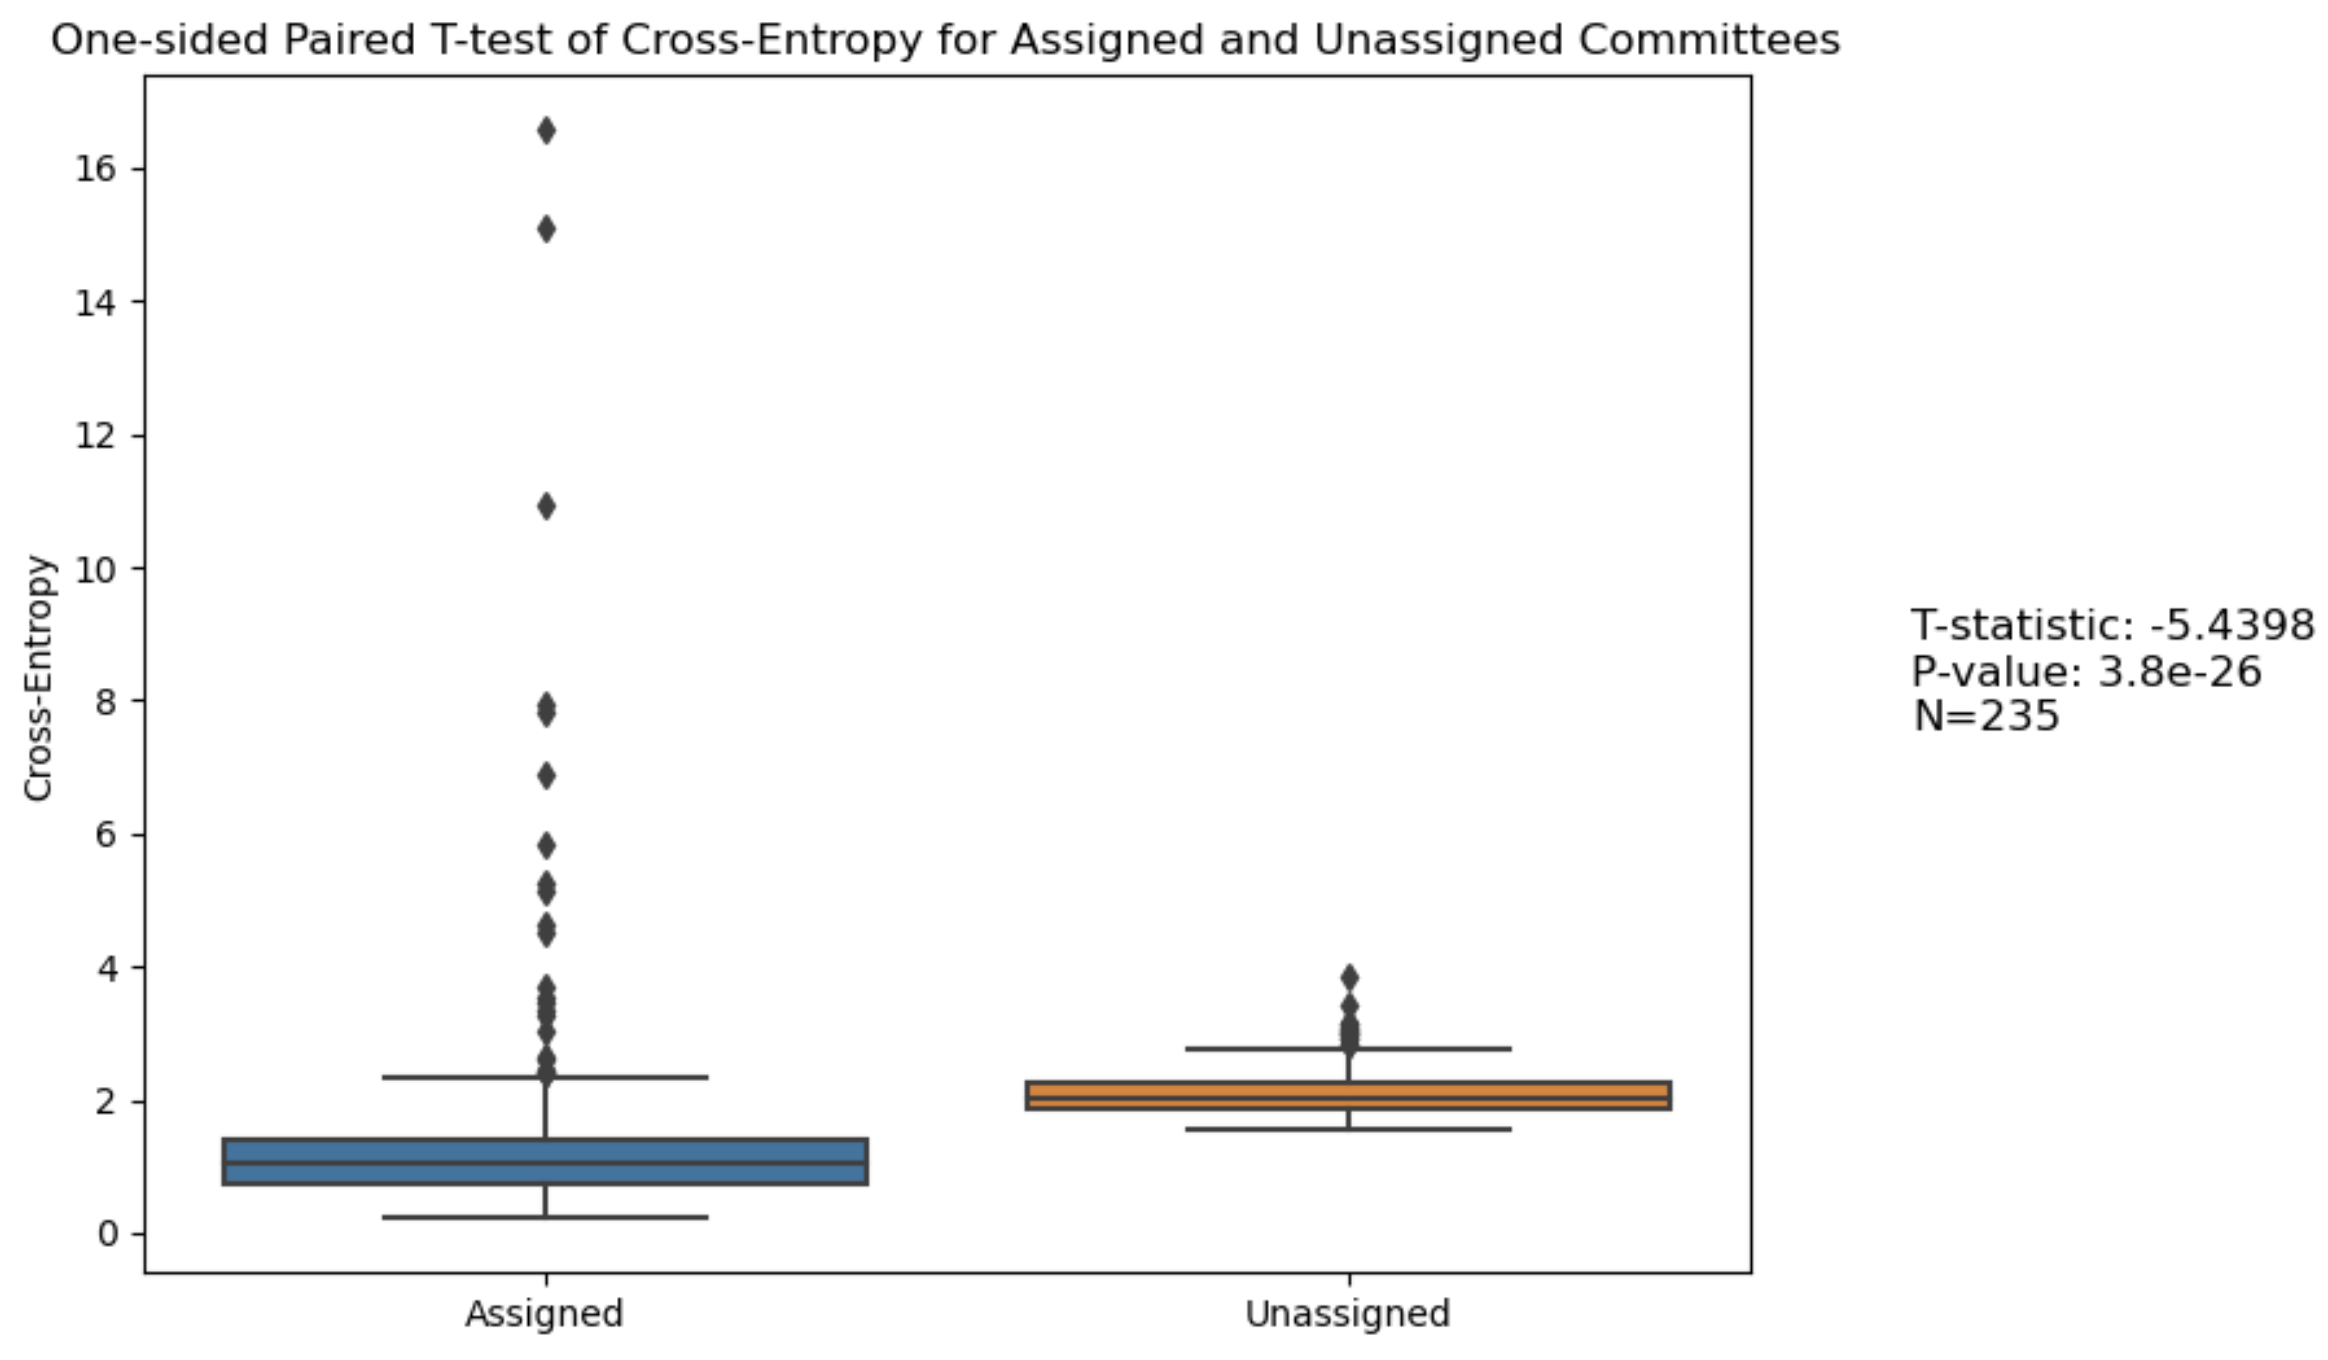
\includegraphics[width=1\textwidth]{imgs/onspt.png}
  \caption{\textbf{One-sided Paired t-test results for the cross-entropy of assigned and unassigned committees.} The figure shows the comparison between the average cross-entropy of assigned and unassigned committees, with a sample size of 235 unique pairs of (Congressperson, Congressional year). The significantly lower average cross-entropy for the assigned group suggests that the stock trading patterns of Congress members more closely resemble the industry distribution of their assigned committees compared to unassigned committees.}
  \label{fig:paired_ttest}
\end{figure}  

\begin{figure}[h!]
  \centering
  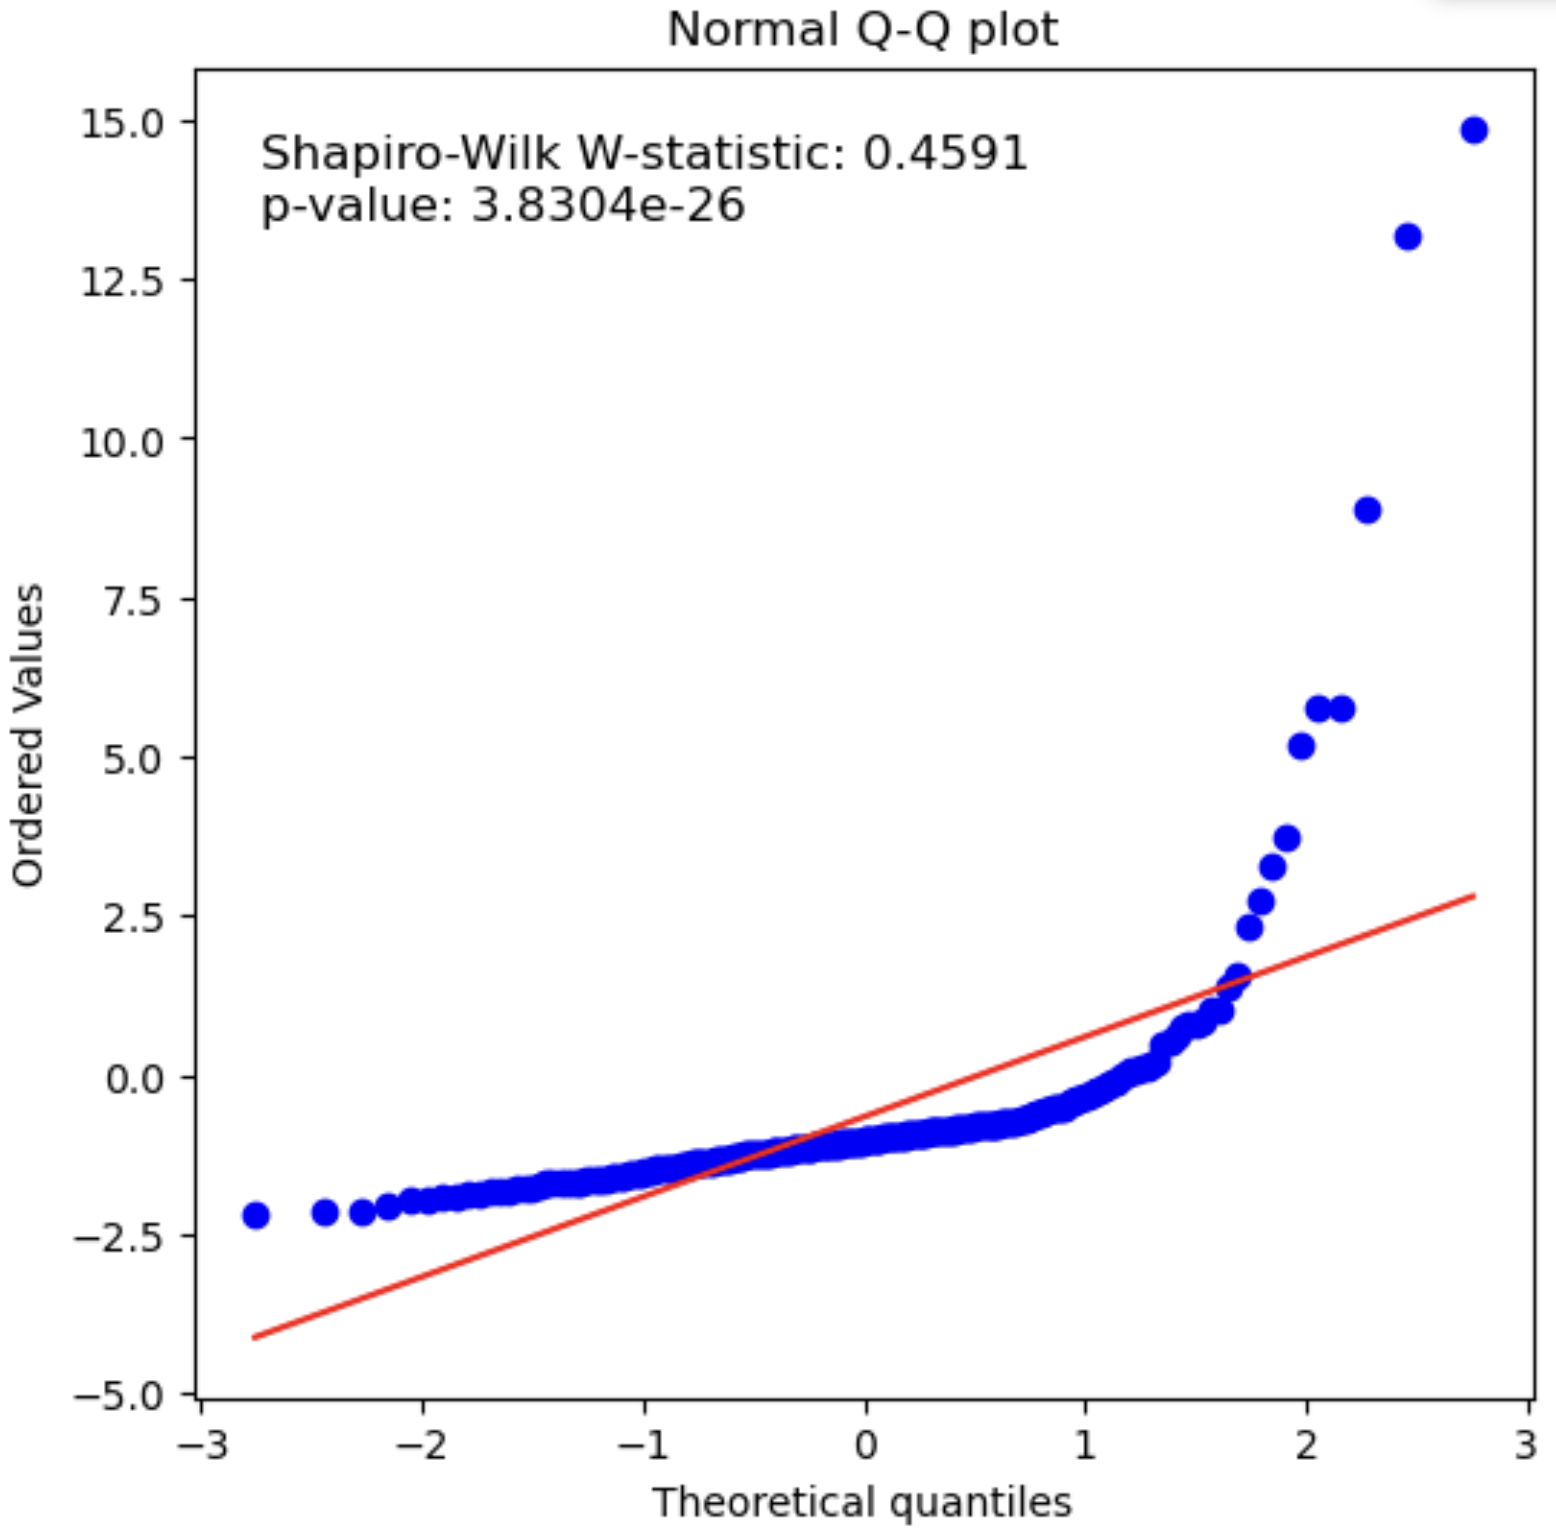
\includegraphics[width=1\textwidth]{imgs/wstat2.png}
  \caption{\textbf{Normal Q-Q plot of the differences in cross-entropy values:} Significantly small p-value of $3.8304 \times 10^{-26}$, decisively rejecting the null hypothesis and suggesting that the differences in cross-entropy are not normally distributed.}
  \label{fig:wstat}
\end{figure}

The results of the one-sided paired t-test are presented in Figure \ref{fig:paired_ttest}, with a sample size of 235 unique pairs of (Congressperson, Congressional year). The statistical test indicates that the average cross-entropy of the assigned committees is significantly lower than that of the unassigned committees. This finding suggests that a Congressperson's stock trading pattern significantly aligns with the industry-level specialization of the committees they are assigned to, supporting the hypothesis that congressional activities influence stock transaction behavior.

The paired t-test used in this analysis is based on several assumptions. Firstly, the data must consist of pairs of observations, where each pair represents a particular entity under two conditions or at two time points. In our case, these pairs consist of average cross-entropy values for each Congressperson for each congressional year, under two conditions: assigned and unassigned committees. This pairing is meaningful as it controls for individual level variation and trends across time, isolating the effect of committee assignment on stock transaction behavior.

Secondly, the paired t-test assumes that the differences between paired observations are independently and identically distributed. In the context of our study, this would mean that the difference in cross-entropy values between the assigned and unassigned committees for a specific Congressperson in a specific Congressional year should be independent of the differences observed for other Congresspersons or other Congressional years.

However, this assumption could potentially be compromised in our setting. Congresspersons often interact and influence each other, potentially leading to correlated trading behaviors. If one Congressperson's stock trading strategy is influenced by another's, this might induce correlations among the differences in cross-entropy values across pairs, thereby potentially violating the assumption of independence.

Additionally, committee assignments are typically influenced by the specialties and expertise of Congresspersons, which can create a potential confounding effect. Since Congresspersons with similar areas of expertise are likely to be assigned to similar committees, the trading patterns influenced by these assignments could become correlated, posing another challenge to the assumption of independence.

Finally, the paired t-test assumes that the differences between paired observations follow a normal distribution. As illustrated in Figure \ref{fig:wstat}, this assumption appears to be violated in our case, with the differences not closely following the reference line in the Q-Q plot.


% The results indicate that the average cross-entropy for the assigned group is significantly lower than that of the unassigned group. This suggests that the stock trading patterns of Congress members more closely resemble the industry distribution of their assigned committees compared to unassigned committees.

Despite the limitations of using a paired t-test, the results indicate that the average cross-entropy for the assigned group is at least descriptively lower than that of the unassigned group. This suggests that the stock trading patterns of Congress members more closely resemble the industry distribution of their assigned committees compared to unassigned committees.
This result is directly opposite to the findings of \cite{eg14}, which conclude that ``\textit{...In contrast, we find no evidence that members disproportionately invest in companies to which they are connected through their committee assignments...}(p.4)''. 
This result, on the other hand, suggests that there exists a clear resemblance between the industry-level bias in Congresspersons' trading and their committees' industry-level specialization.
% This result, on the other hand, suggests that committee assignments affect the congresspersons' decisions to invest disproportionately in industries connected to their committee assignments.


There could be several reasons for this discrepancy. For example, the data range is different: \cite{eg14} consider the period from January 1, 2004, to December 31, 2008, while in this case, we consider the 115th, 116th, and 117th Congresses, which correspond to the years 2017 to 2022. However, more fundamentally, the difference may reside in the measurement approach.

\cite{eg14} use a binary encoding to indicate whether a specific firm has engaged in lobbying behavior on a certain bill that is referred to a particular congressional committee. They then design a linear regression model to predict the weight of that specific firm's stock in a congressperson's entire investment portfolio. In this way, they investigate whether there is a relationship between a firm's lobbying activities on bills assigned to a committee and the investment decisions of congresspersons who are members of that committee. However, this approach only captures a specific company's lobbying behavior rather than industry-level information in its entirety. For example, multiple firms can lobby on the same bill assigned to a certain committee, then a congressperson on that committee can evaluate more broadly how this could impact the industry as a whole and selectively redesign their own portfolio. This means that there is no reason to assume that a congressperson would buy a specific stock that is being lobbied for — instead, it is more plausible to understand that such lobbying provides more detailed context about a specific industry, which the congressperson can utilize in their personal financial investment decisions.

Therefore, while the cross-entropy approach, which directly measures the industry-level similarity between a committee's interests and a congressperson's portfolio, provides a more intuitive and comprehensive understanding of the potential influences on a congressperson's investment behavior, it is not without limitations. The approach allows us to discern a relationship between the industry-level specialization of committee assignments and the industry-level bias in Congresspersons' stock trading, which contributes to our understanding of these influences. However, it is important to recognize that confounding factors could affect both committee assignments and the resemblance of stock trading to the committee's industry-level specialization.
For example, scholarly consensus suggests that committee assignments are often based on a congressperson's existing knowledge and expertise \citep{10.2307/40709444, 10.2307/2111156, kiewiet1991logic, krehbiel1992information, curry2018knowledge}. Consequently, it's possible that the observed correlation between a congressperson's trading patterns and their committee's industry specialization may not entirely result from knowledge gained through congressional activities, but may also be influenced by pre-existing expertise and interests. This introduces a confounding factor, making it challenging to disentangle the effects of pre-existing expertise from the potential influence of congressional committee assignments on trading decisions. The relationship between a congressperson's industry specialization, their committee assignments, and their stock trading patterns thus warrants further exploration and calls for more nuanced analysis.

Another potential limitation of this analysis is the difficulty in collecting NAICS codes for ETFs and Mutual Funds, which comprise approximately 60\% of the stock transactions in our dataset. Although each ETF or Mutual Fund's website provides information about their holdings, it was challenging to establish a generalizable pattern across different providers to obtain the composition of stocks held by these funds and their corresponding NAICS codes. Consequently, this section focuses on individual stocks and their corresponding NAICS codes, which might not fully capture the reality of Congress members' investments. However, the findings still indicate that the individual stock trading behaviors of Congress members are significantly influenced by their assigned committees.

In addition to our primary findings, it's important to acknowledge an interesting observation from Figure \ref{fig:paired_ttest}: the variance in average cross-entropy for assigned committees is considerably higher than that for unassigned committees. This suggests that the stock trading behavior of a subset of Congresspersons deviates significantly from the industry specialization of their assigned committees. This pattern opens up a fascinating potential interpretation.

The conventional political science theory posits that the primary motivation for congressional members is re-election \citep{Mayhew1975CongressTE,fenno1977}. From this perspective, Congresspersons might demonstrate caution in selecting stocks to trade to avoid the perception of conflict of interest with their assigned committees' focus industries. Essentially, they may strive to prevent any appearance of using insider knowledge gained from committee assignments for personal financial gain, which could negatively affect their chances of re-election. This behavior underscores the importance of considering not just direct legislative and financial interests but also political strategy and public perception in understanding the investment behavior of Congresspersons.



\section{Predicting Congressional Stock Transactions using Graph Neural Networks}\label{sec:gnn}

In the previous section, therefore, I discussed the limitations of the linear prediction model used by \cite{eg14}, which employed a binary encoding of lobbying and committee assignments to predict the weight of a specific firm's stock in a congressperson's portfolio. I pointed out that this model did not fully capture the complex interactions between different entities involved in congressional activities, particularly at the industry level. However, I acknowledge that the model was an attempt to explain congressional stock transactions using potentially explanatory components such as district, PAC, lobbying, and committee assignments.

It's important to note that while the cross-entropy approach in Section \ref{sec:ce} revealed a clear resemblance between Congresspersons' stock trading behavior and their assigned committees' industry-level specialization, this approach does not directly answer whether this resemblance originates from knowledge gained through congressional activities or from the Congresspersons' expertise and experience before their congressional tenure. 
% Hence, although our model provides valuable insights, it still has its own limitations. It would be an oversimplification to attribute the observed resemblance solely to either pre-congressional expertise or congressional activities, as the reality likely involves a complex interplay of both factors. This calls for a more nuanced model that can further decompose and understand these influences.

In this section\footnote{Reproducible code for this section is available at \url{https://github.com/syyunn/gnnex/blob/main/hetero/train_kfold_auto.py}}, I propose to use a graph neural network (GNN) \citep{gnn1, gnn2, gnn3, gnn4} to predict congressional stock transactions using the information embedded in the congressional activities captured in the data explained in Section \ref{sec:data}. The GNN approach is uniquely equipped to handle this task because it can model the complex relationships among various entities involved in congressional activities, all of which are naturally structured as a graph.

By using GNN, we can design a model that directly consumes the congressional graph that captures legislative-related activities of different entities, thereby enabling us to test the predictability of congressional trading behavior based on these activities. This will help us isolate the influence of congressional activities on stock trading from pre-congressional expertise and other confounding factors, which is a significant step forward in our understanding of the interplay between committee assignments, congressional activities, and stock transactions.
By leveraging a graph representation of the relationships between firms, bills, committees, and congresspersons, we can train a GNN to predict whether a congressperson is likely to buy a particular stock. 

% This will enable us to investigate whether there is an associational relationship between congressional activities and stock transactions, and to identify the most relevant types of interactions between entities that contribute to the predictions.

% While \cite{eg14}'s linear prediction model attempted to explain congressional stock transactions using a limited set of explainable components, the GNN approach will enable us to capture the complexity of the relationships between different entities involved in congressional activities. This will provide new insights into the potential influence of congressional activities on stock transactions and complement the findings of previous studies.

The advantage of using a Graph Neural Network (GNN) over a traditional approach such as including industry dummy variables in a regression model can be attributed to several reasons.


Firstly, a GNN can integrate complex interactions between entities along with their inherent attributes simultaneously in a way that traditional regression models can't accomplish. In our case, we have a multitude of entities such as Congresspersons, committees, bills, industries, and stocks, each with their unique characteristics, represented as node-level attributes in the graph. Additionally, their relationships, expressed as edges in the graph, embody another layer of intricate information. By modeling these entities and their interactions as a graph and applying GNN, we can concurrently consider node attributes and graph topology, enabling a more nuanced understanding of the congresspersons' decision-making processes in their stock transactions. This holistic approach of GNN allows us to capture these complex relationships in a more natural and efficient way.

Secondly, GNNs can better handle the heterogeneous and high-dimensional nature of our data. A traditional approach using industry dummy variables is limited in its ability to handle high-dimensional categorical variables. Furthermore, this approach treats each industry as a separate and independent entity, ignoring any potential correlations or dependencies between industries. On the other hand, GNNs can handle high-dimensional data and also account for the interconnectedness of entities.

Finally, GNNs are capable of learning and evolving over time, allowing them to adapt and improve their predictions as new data comes in. This is especially useful in our context, where the behavior and preferences of Congresspersons, the focus of committees, and the performance of industries and stocks can change over time.

In conclusion, using GNNs to predict congressional stock transactions provides a more nuanced and dynamic understanding of the intricate relationships among various entities involved in congressional activities, leading to more accurate predictions.

\subsection{Designing a Binary Classifier with Graph Neural Networks}

To predict congressional stock transactions using a graph neural network (GNN) approach, I design a binary classifier that takes as input a graph $G$, a congressperson and a ticker (stock symbol). The classifier, denoted as $f(G, \text{congressperson}, \text{ticker})$, will output a binary prediction of either 0 or 1, indicating whether an edge (a buy or sell relationship) exists between the given congressperson and the ticker.

The hidden representations \citep{hd1, hd2}o f the congressperson and the ticker, denoted as $h_{\text{congressperson}}$ and $h_{\text{ticker}}$ respectively, are obtained as outputs of the GNN model. The main task in this approach is to train the GNN model to learn a computational graph that generates ``good'' representation of the congressperson and the ticker, $h_{congressperson}$ and $h_{ticker}$, which involves how to effectively encode the information embedded in the network to perform the downstream task of binary classification \citep{hdforc}.

To design the classifier, a probabilistic modeling approach is used that comprises of a sigmoid function applied to the logit, which is the output of the model. The logit of the model is obtained by passing the representation learned by the GNN, $h_{congressperson}$ and $h_{ticker}$, to an MLP (Multi-layer perceptron) \citep{Gardner1998ArtificialNN, 7103337} that maps the representations of the congressperson and the ticker to a single logit. In other words, the MLP takes as input the representations of the congressperson and the ticker learned by the GNN, and outputs a logit that will be used to compute the probability of the existence of edge between them. MLP is simply an affine transformation over the concatenation of two representations, $h_{congressperson}$ and $h_{ticker}$, follwed by a non-linear activation function \citep{nonl}, which is ReLU \citep{relu} in this case.

Formally, the logit of the classifier is defined as:

% \begin{align*}
%   \operatorname{logit} &= \operatorname{MLP}\left(h_{\text{congressperson}}, h_{\text{ticker}}\right) \\
%   \operatorname{where} \; \operatorname{MLP}(x) &= \operatorname{ReLU}(Ax + b) \\
%   x &= \operatorname{concat}\left(h_{\text{congressperson}}, h_{\text{ticker}}\right) \\
%   A &\in \mathbb{R}^{(d+d) \times 1} \\
%   b &\in \mathbb{R}^{1}
% \end{align*}

\begin{align*}
  \operatorname{logit} &= \operatorname{MLP}\left(x\right) \operatorname{ where }\\  
  \operatorname{MLP}(x) &= \operatorname{ReLU}(Ax + b) \\
  x &= \operatorname{concat}\left(h_{\text{congressperson}}, h_{\text{ticker}}\right) \\
  A &\in \mathbb{R}^{(d+d) \times 1} \\
  b &\in \mathbb{R}^{1}
\end{align*}
  
  $\boldsymbol{\cdot}\operatorname{logit}$: This is the output of the model. It's a transformed version of the probability that a congressperson would invest in a particular stock. In this binary classification problems, the logit (also known as log-odds) is the logarithm of the odds p/(1-p) where p is the probability of a positive event that congressperson trades such stock.
  
  $\boldsymbol{\cdot} \operatorname{MLP}$: This stands for Multi-Layer Perceptron, a type of artificial neural network. In this case, it's a function that takes the concatenated embeddings of a congressperson and a ticker as input and produces a logit as output.
  
  $\boldsymbol{\cdot} h_{\text{congressperson}}$, $h_{\text{ticker}}$: These are the vector embeddings of a congressperson and a ticker symbol, respectively. Each vector embedding represents the congressperson or ticker in the learned feature space. The embeddings are of dimension $d$.
  
  $\boldsymbol{\cdot} \operatorname{ReLU}(Ax + b)$: This is a Rectified Linear Unit activation function applied to a linear transformation of the input. ReLU is defined as $\operatorname{ReLU}(x) = \max(0, x)$ and is used to introduce non-linearity into the model.
  
  $\boldsymbol{\cdot}$  $\operatorname{concat}$: This is a function that concatenates (joins together) two vectors. Here, it concatenates the embeddings of a congressperson and a ticker symbol into a single vector of shape $1 \times 2d$, where $d$ is the dimension of the individual embeddings. This shape is designed to be compatible with the weight matrix $A$ which is of shape $2d \times 1$.
  
  $\boldsymbol{\cdot} A$: This is a weight matrix for the linear transformation in the MLP. It's of shape $(d+d) \times 1$, meaning it takes a vector of size $2d$ and transforms it to a vector of size $1$.
  
  $\boldsymbol{\cdot} b$: This is a bias term for the linear transformation in the MLP. It's added to the output of the linear transformation before the ReLU activation is applied.
  
  $\boldsymbol{\cdot} d$: This represents the dimensionality of the vector embeddings of the congressperson and ticker. $d+d$ is therefore the dimensionality of the concatenated input vector.
    
The sigmoid function is then applied to the logit to obtain a probability value:

$$
\text { prob }=\sigma(\text { logit })
$$

where $\sigma(x)$ is the sigmoid function. The probability value indicates the likelihood of an edge existing between the given congressperson and the ticker. If the probability value is above a certain threshold, we predict that an edge exists between them, otherwise we predict that there is no edge.

Then remaining task is how to design a GNN model that can effectively learn the representations of the congressperson and the ticker, $h_{\text{congressperson}}$ and $h_{\text{ticker}}$, respectively, which can be used to train the classifier. In the following section, I will discuss the design of the GNN model.

\subsection{Design of the Graph Neural Network Architecture}

To obtain the representations $h_{\text{congressperson}}$ and $h_{\text{ticker}}$, I use a GNN approach that is designed to handle the complexity and dynamics of the congressional graph. The GNN approach is based on the idea of message passing and updating \citep{gnn1, gnn2}, which is a process of aggregating information from the neighbors and updating the representation of each node accordingly.

In the case of the congressional graph, I use an edge-conditioned convolution GNN model \citep{nnconv1, nnconv2}, which takes into account the edge attributes, such as the date, to better capture the complex relationships in the graph. The message passing, aggragation and updating in this model is defined as:

$$
\mathbf{h}_i^{\prime}=\boldsymbol{\Theta} \mathbf{h}_i+\sum_{j \in \mathcal{N}(i)}  \mathbf{MLP}\left(\mathbf{e}_{i, j}\right) \cdot \mathbf{h}_j
$$

where $\mathbf{h}_i$ and $\mathbf{h}_j$ are the representations of nodes $i$ and $j$, respectively, $\mathbf{e}_{i,j}$ is the edge attribute between nodes $i$ and $j$, $\mathcal{N}(i)$ is the set of neighbors of node $i$, $\boldsymbol{\Theta}$ is a learnable matrix of size $d \times d$, where $d$ is the dimension of the representation space, and $\mathbf{MLP}$ takes the edge attribute $\mathbf{e}_{i,j}$ as input and outputs a weight matrix of size $d \times d$. 
This weight matrix is then multiplied with the representation $\mathbf{h}_j$ of the neighbor node $j$ to obtain a message $\mathbf{m}_{i,j}= \mathbf{M L P}\left(\mathbf{e}_{i, j}\right) \cdot \mathbf{h}_j$. In the updating step, the message from each neighbor node is aggregated by summing them up, and the resulting sum is added to the current representation $\mathbf{h}_i$ of node $i$ multiplied by the learnable parameter matrix $\boldsymbol{\Theta}$ to obtain the updated representation $\mathbf{h}_i^{\prime}$.

In the case of the congressional graph, the edge attribute $\mathbf{e}_{i,j}$ represents the relationship between nodes $i$ and $j$ at a specific date, which is represented as the elapsed time from a reference date (in this case, January 1, 2016). 
However, in our case, we have different types of edges, which means that $\mathbf{MLP}\left(\mathbf{e}_{i, j}\right)$ should be differently defined for different types of edges. This is because parsing the information of start and end dates should be considered differently across different edge types. For example, committee assignments of a congressperson that occurred over a specific congressional year should be considered differently from the date information that a certain firm lobbied on a certain bill. To account for this, I used the expanded version of the above formula:

$$\mathbf{h}_i^{(l+1)}=\boldsymbol{\Theta}^{(l)} \mathbf{h}_i^{(l)}+\sum_{j \in \mathcal{N}(i)} \operatorname{MLP}^{(l)}_k\left(\mathbf{e}_{i, j}^{(k)}\right) \cdot \mathbf{h}_j^{(l)}$$

Here, $l$ represents a layer, and we can expand the expressivity of such message passing and updating process by stacking up the repeated layers of this operation. This allows the model to learn a more complex representation of each node, which is essential for capturing the intricate relationships in the congressional graph.
Experimentally, I found that using 2 layers of message passing and updating was sufficient to learn the best representation of each node and used this configuration for the GNN model.

In conclusion, our GNN aims to learn the optimal parameter set that defines $\boldsymbol{\Theta}^{(l)}$ and $\operatorname{MLP}_k^{(l)}$ to output the best representations $\mathbf{h}_i^{(l)}$ and $\mathbf{h}_j^{(l)}$, which helps to perform the downstream task successfully. In this case, the downstream task is generating the best logit in the prediction head, $\operatorname{MLP}(\mathbf{h}_{\text{congressperson}}, \mathbf{h}_{\text{ticker}})$. It is important to note that the representations $\mathbf{h}_i^{(l)}$ and $\mathbf{h}_j^{(l)}$ are initialized randomly before they are provided into the first layer of the message passing and updating process. Through multiple rounds of message passing and updating, the GNN is tuned to output the best representation of each node that scores the best performance as possible in binary classification of edge existence.

\subsection{Training \& Evaluation of the GNN}
\subsubsection{Dataset Preparation}

In the context of our GNN architecture, the goal is to predict the existence of edges between two nodes, a task commonly known as link prediction. To train the GNN for this task, the dataset must be prepared for training and evaluation (test). The dataset consists of a total of 24,675 edges, which represent the relationship (congressperson, buy-sell, ticker).

To create a balanced dataset for the link prediction task, the dataset is divided into a train and test set with an 8:2 ratio, resulting in 19,740 instances for training and 4,935 instances for testing. The network is then trained using the 19,740 instances and its performance is evaluated on the 4,935 test instances.

In addition, to ensure a balanced dataset, the same number of randomly sampled negative edges \citep{nns} is prepared. These negative edges are created by randomly selecting pairs of nodes (congressperson and ticker) that do not have a connection in the original dataset. This results in a total of 39,480 edges for training and 9,870 edges for testing. Including both positive and negative examples in the training process helps the model to better differentiate between true and false existence of edges between congressperson and tidcker nodes, improving its ability to predict links in the graph.

\subsubsection{Training of the GNN}

For the training of the GNN, a two-layer GNN architecture, as $l=2$, is employed. Additionally, node embeddings $h_i$ are represented as vectors in a 64-dimensional space ($h \in \mathbf{R}^{64}$). This hyperparameter is also set experimentally.

In order to measure the performance of the model during the training process, binary cross-entropy loss is used as the loss function. Binary cross-entropy loss is particularly suitable for binary classification problems \citep{bcsec}, such as link prediction \citep{lp}, where the goal is to differentiate between the presence and absence of a connection between two nodes. This loss function quantifies the difference between the predicted probabilities and the true labels, and penalizes the model for incorrect predictions. Formally, the binary cross-entropy loss for a set of samples is defined as:

$$L=-\sum_{i=1}^N\left(y_i \cdot \log \left(p_i\right)+\left(1-y_i\right) \cdot \log \left(1-p_i\right)\right)$$

where $L$ represents the total binary cross-entropy loss.
$N$ is the total number of samples.
$y_i$ is the true label for the $i$th sample (1 for the presence of a connection, and 0 for the absence of a connection).
$p_i$ is the predicted probability of a connection existing between two nodes for the $i$th sample.

By minimizing the binary cross-entropy loss, the GNN learns to accurately predict the existence or non-existence of links in the network, ultimately improving its performance on the link prediction task.
For the minimization, the Adam optimizer \citep{kingma2014adam} with stochastic gradient descent (SGD) is utilized. SGD is an iterative optimization algorithm that updates the model's parameters based on a random sample (or minibatch) of training data in each iteration \citep{AMARI1993185}. This approach helps in converging faster and reduces the impact of noisy gradients, thus improving the optimization process. Adam is an adaptive learning rate optimization algorithm, combining the advantages of two other popular optimization methods, AdaGrad and RMSProp \citep{kingma2014adam}. This optimizer is well-suited for large-scale problems and is known for its ability to efficiently handle noisy and sparse gradients, making it a suitable choice for training GNNs.

To obtain a more robust estimation of the model's performance and uncertainty, a 5-fold cross-validation \citep{elem} is performed. In this approach, the entire dataset is randomly split into five equal-sized chunks. For each fold, one chunk is used as the test set, while the remaining chunks are combined to form the training set. This process is repeated five times, with each chunk being used once as the test set. This technique allows for a better understanding of the model's performance across different subsets of the dataset and provides uncertainty statistics of overall prediction performance.

\subsubsection{Evaluation \& Ablation Study}

In this study, we conducted a link-prediction \citep{lp} task to predict the existence of an edge between a congressperson and a ticker, symbolizing the trade relationship - whether the given congressperson would sell or buy a particular stock. This task was performed using a variety of edge types, and the performance was evaluated using two metrics: accuracy and Area Under the Receiver Operating Characteristic Curve (AUC-ROC).

The results of this evaluation are depicted in Figures \ref{fig:accuracy_drop} and \ref{fig:auc_roc_drop}. With all edge types included, the model achieved an accuracy of approximately 81\% and an AUC-ROC of 0.89. These results indicate that the model was generally effective at predicting the stock transactions of congresspersons.

To further understand the importance of each edge type, I conducted an ablation study, where I systematically removed each edge type from the training and testing data and observed the resulting performance drop. The most significant drop in performance was observed when the edge type (`congressperson', `assignment', `committee') was removed. This resulted in a decrease in accuracy from 81\% to 67\%, and a decrease in AUC-ROC from 0.89 to 0.76. This suggests that the (`congressperson', `assignment', `committee') edge type carries significant information for predicting a congressperson's stock transactions.

In comparison, the removal of other edge types, such as (`bill', `assigned\_to', `committee'), or (`ticker', `lobbies\_on', `bill'), resulted in less dramatic performance drops. This further underscores the relative importance of the (`congressperson', `assignment', `committee') edge type in this prediction task.


\begin{figure}[h!]
  \centering
  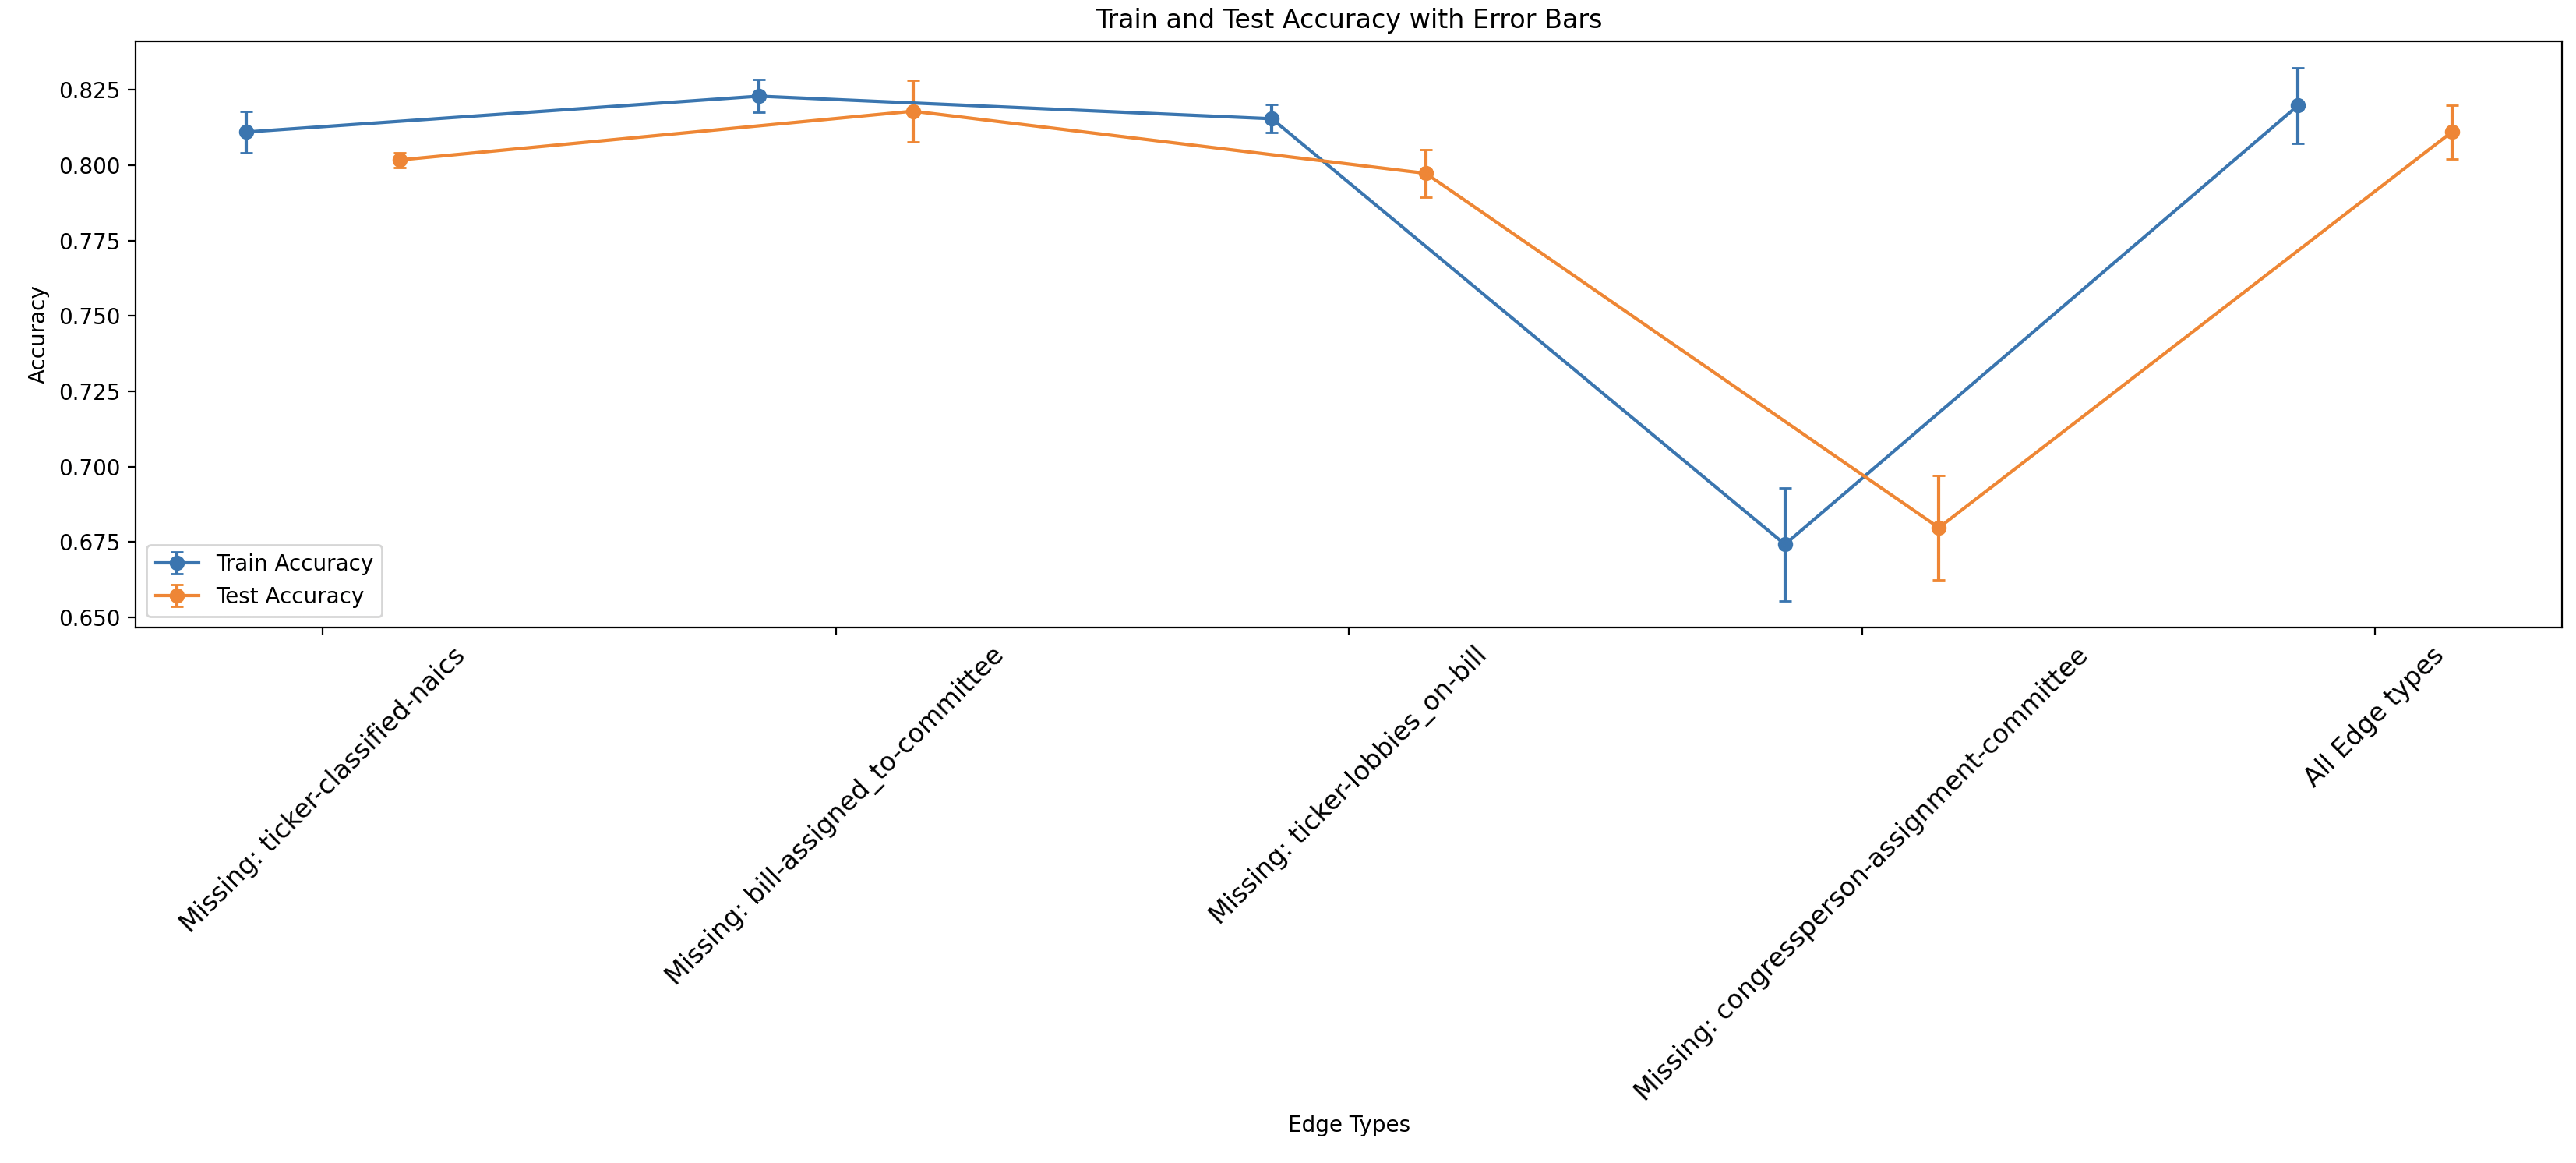
\includegraphics[width=1.1\textwidth, height=0.4\textheight]{imgs/acc2.png}
  \caption{\textbf{Accuracy drop for different edge types.} The figure shows the accuracy of the model with all edge types included and with each edge type removed one at a time. With all edge types included, the model achieved an accuracy of approximately 81\%. The most significant drop in accuracy, to 67\%, was observed when the edge type (`congressperson', `assignment', `committee') was removed. This suggests that the (`congressperson', `assignment', `committee') edge type carries significant information for predicting a congressperson's stock transactions.}
  \label{fig:accuracy_drop}
\end{figure}  

\begin{figure}[h!]
  \centering
  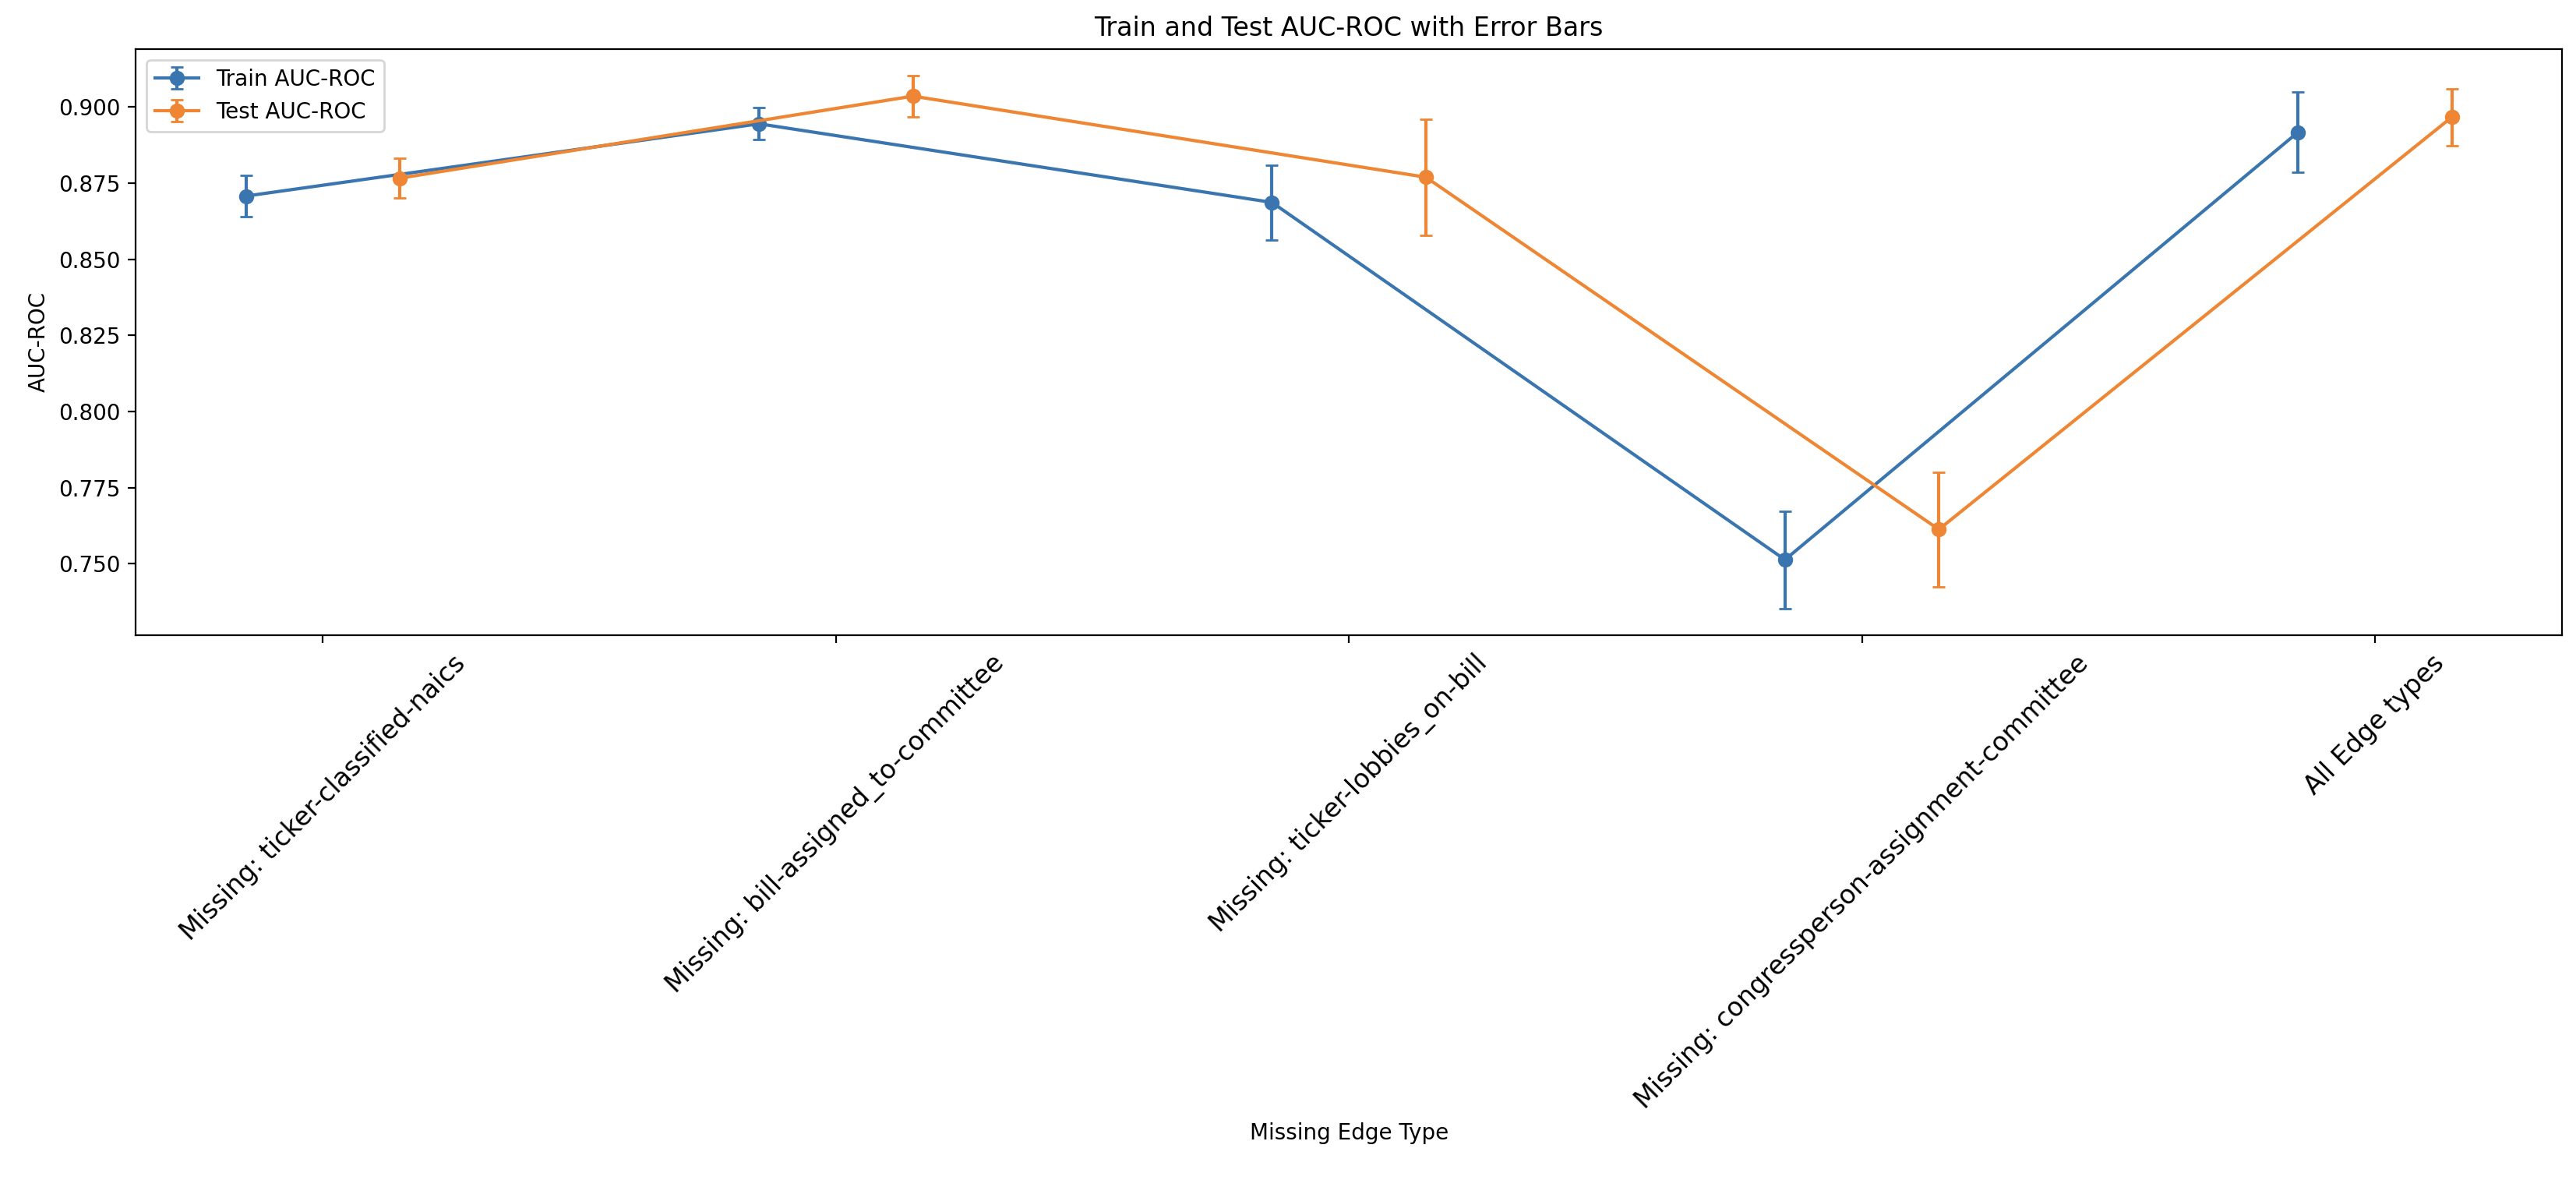
\includegraphics[width=1.1\textwidth, height=0.4\textheight]{imgs/auc2.png}
  \caption{\textbf{AUC-ROC drop for different edge types.} The figure shows the AUC-ROC of the model with all edge types included and with each edge type removed one at a time. With all edge types included, the model achieved an AUC-ROC of approximately 0.89. The most significant drop in AUC-ROC, to 0.76, was observed when the edge type (`congressperson',`'assignment', `committee') was removed. This suggests that the (`congressperson', `assignment', `committee') edge type carries significant information for predicting a congressperson's stock transactions.}
  \label{fig:auc_roc_drop}
\end{figure}

To further quantify the importance of each edge type, I employed the concept of Shapley values \citep{shapley1,shapley2,shapley3}, a concept borrowed from cooperative game theory. In this context, each edge type can be considered as a player in a cooperative game, where the ``payout'' is the performance of the model.

$$
\varphi_i(v)=\sum_{S \subseteq N \backslash\{i\}} \frac{|S| !(n-|S|-1) !}{n !}(v(S \cup\{i\})-v(S))
$$

Here, $\varphi_i(v)$ is the Shapley value for edge type $i$, representing the average marginal contribution of edge type $i$ to the performance of the model, considering all possible combinations of edge types. $N$ is the set of all edge types, not the total number of edges. In our case, there are four edge types, so $N$ is 4. $S$ is a subset of $N$ that does not include edge type $i$, $|S|$ is the number of edge types in subset $S$, and $n$ is the total number of edge types. $v(S \cup{i})$ and $v(S)$ represent the performance of the model when edge type $i$ is added to and excluded from the subset $S$ of edge types, respectively. This means that the Shapley value indicates how much each edge type contributes to the performance of the model, which in our case is measured by prediction accuracy or AUC-ROC.

The Shapley values were computed over all $16 (=2^4)$ possible combinations of the four different edge types, with each combination evaluated through a five-fold cross-validation process. The uncertainty associated with each Shapley value, as reflected in the standard deviation across the five folds, provides an indication of the stability of the Shapley value estimates. The results of this analysis are shown in Figure \ref{fig:shap_values}.

These findings indeed underline the crucial role of the (congressperson', assignment', `committee') edge in predicting congresspersons' stock transactions. Nevertheless, it's worth noting that these results are contextually bound to our graph design. The importance of committee assignments in predicting stock transactions might be somewhat overemphasized due to the absence of other possible edges connecting congresspersons to stocks, such as bill co-sponsorship, business relations, or previous occupation. Including additional edges reflecting other aspects of congressional activities in future work might provide a more nuanced view of the importance of committee assignments and other factors in predicting congresspersons' stock trading behavior."

\begin{figure}[h!]
  \centering
  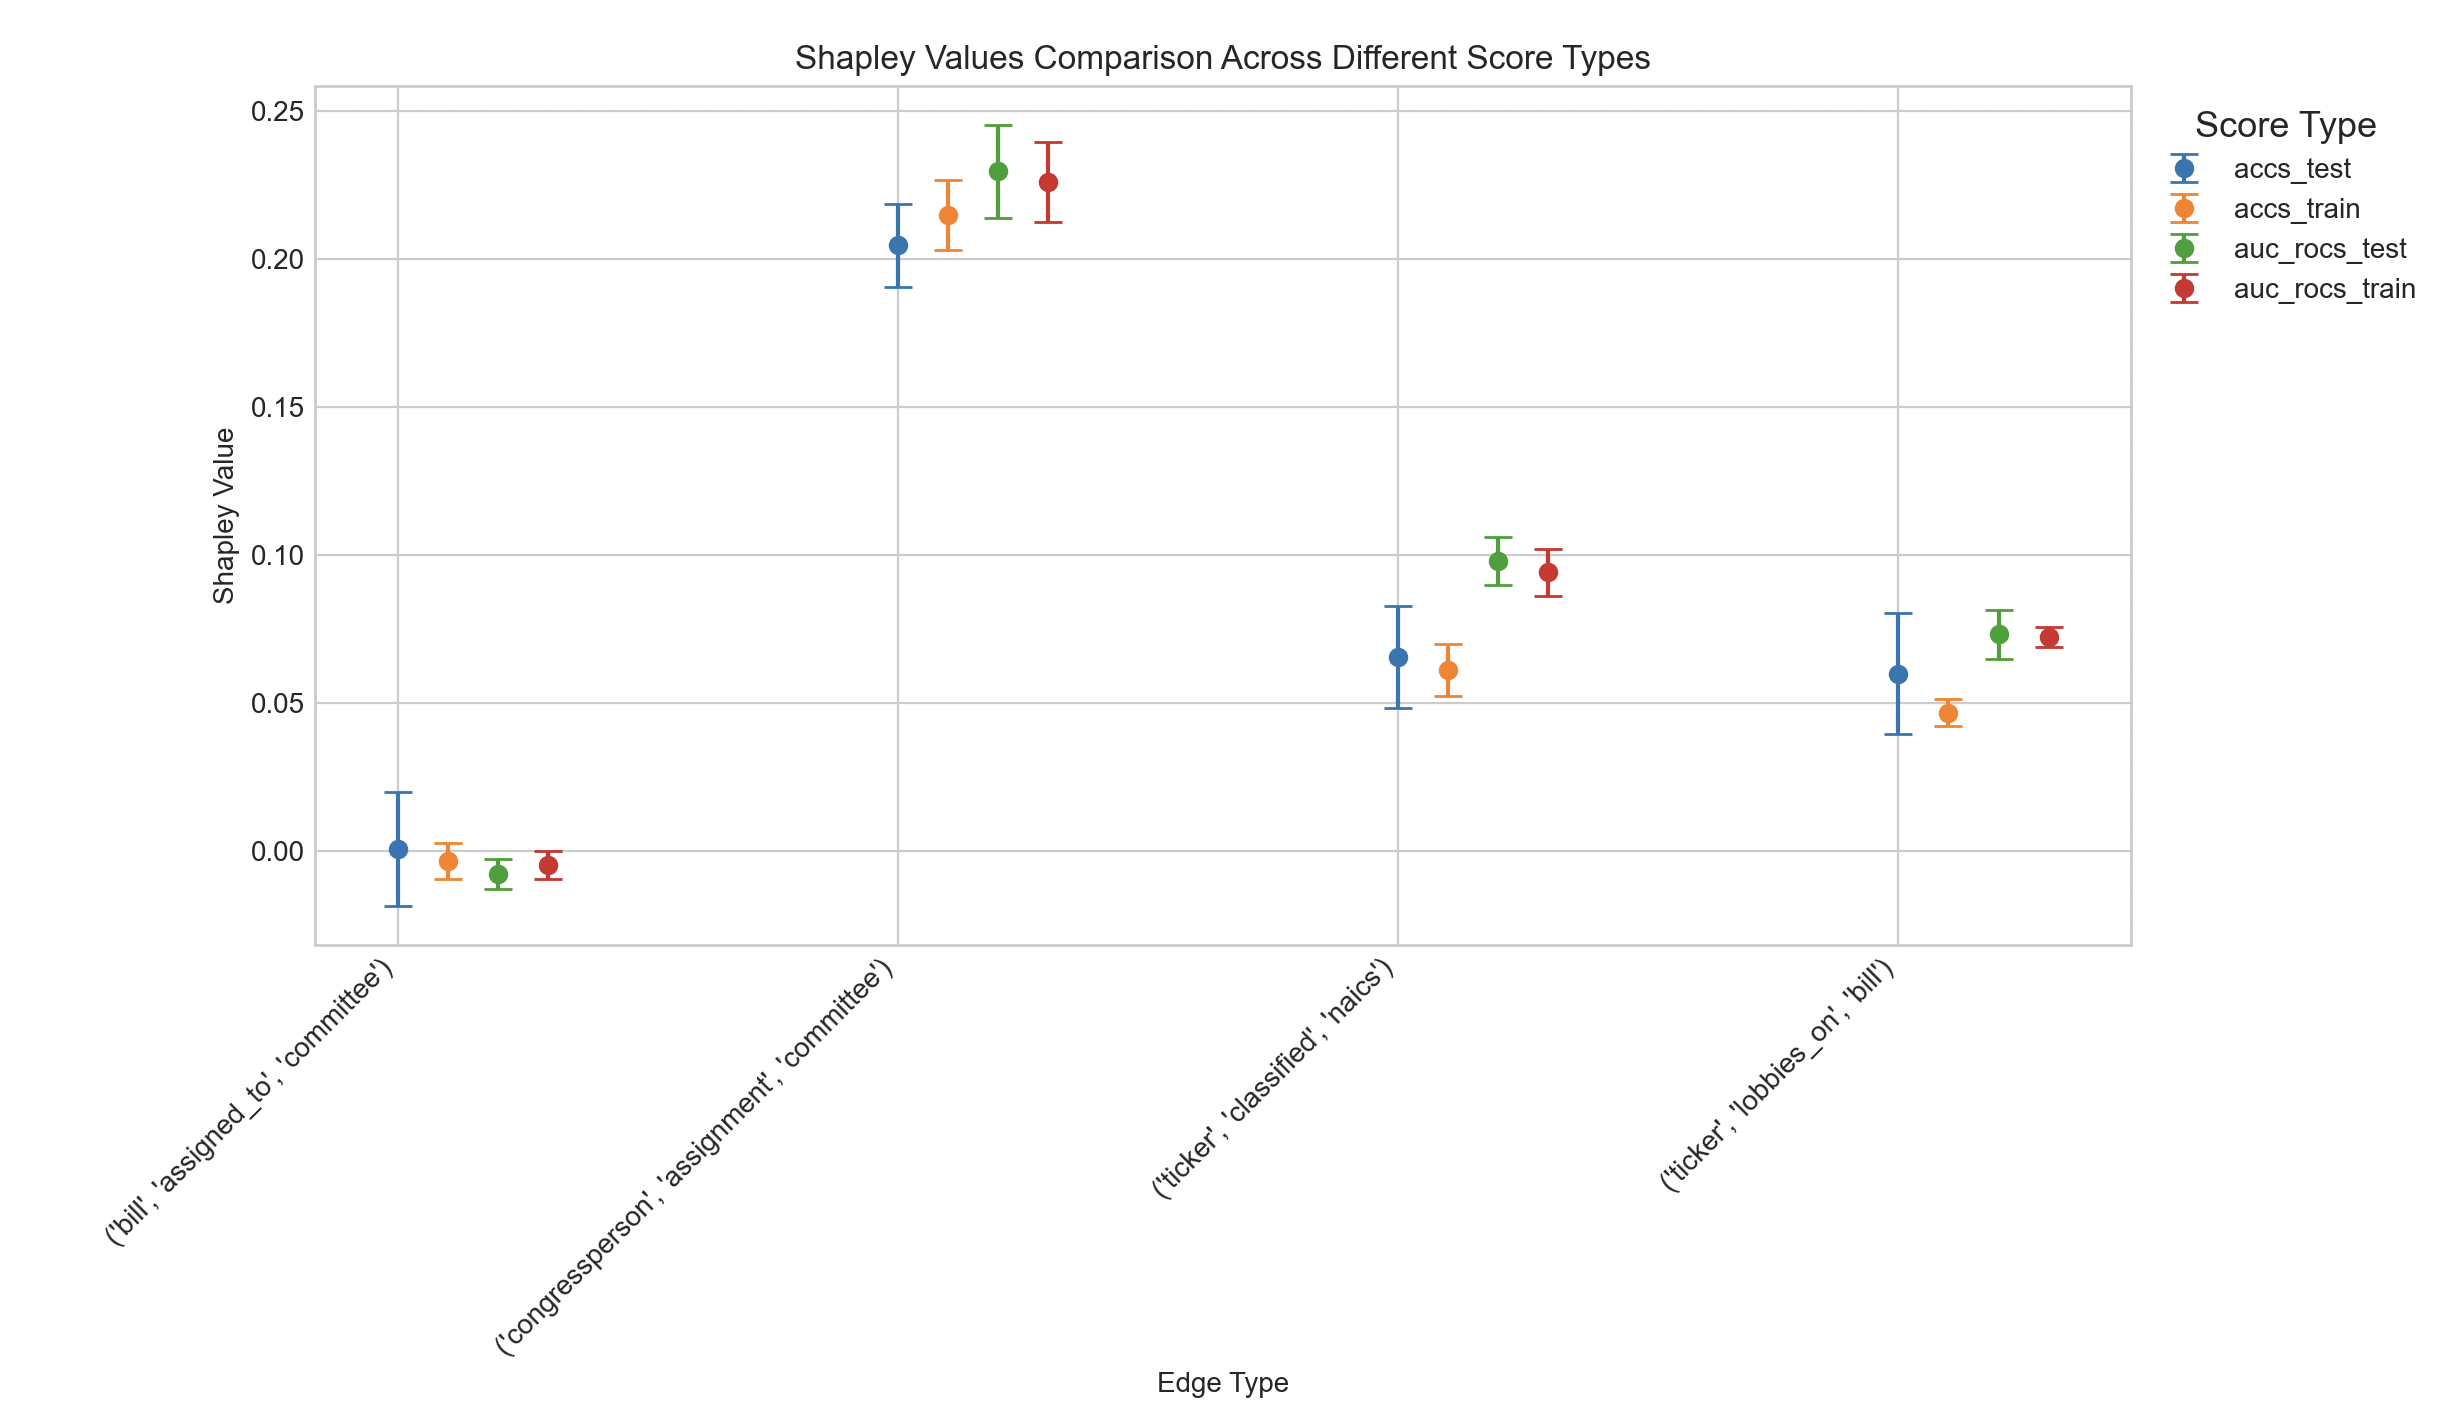
\includegraphics[width=1.1\textwidth, height=0.4\textheight]{imgs/shapeee.png}
  \caption{\textbf{Shapley values for different edge types.} The figure shows the Shapley values for each edge type, computed over all $16 (2^4)$ possible combinations of the four different edge types. The Shapley value for an edge type represents its average marginal contribution to the performance of the model, considering all possible combinations of edge types. The most important feature, according to the Shapley value analysis, was (`congressperson', `assignment', `committee'), followed by (`ticker', `classified\_as', `naics') and (`ticker', `lobbies\_on', `bill'). This further reinforces the conclusion that the (`congressperson', `assignment', `committee') edge type plays a crucial role in predicting congressperson's stock transactions.}
  \label{fig:shap_values}
\end{figure}

In the Shapley value analysis, I observed that the edge type (`bill', `assigned\_to', `committee') had a Shapley value of zero or even negative. This suggests that this type of edge does not contribute to increasing the performance of the model. In fact, it appears to harm the performance when included.

% Given that our task is to predict the existence of a link (edge) between a given congressperson and a ticker, this result implies that most of the relevant information for a congressperson comes from the edge type ('congressperson', 'assigned\_to', 'committee'), and most of the relevant information for a ticker comes from the edge types ('ticker', 'classified\_as', 'naics') and ('ticker', 'lobbies\_on', 'bill').

The reason for the zero or negative contribution of the edge type (`bill', `assigned\_to', `committee') is not immediately clear and warrants further investigation. 
One possible explanation could be that bills can be assigned to different committees, making this information more complex and potentially harder for the model to utilize effectively. 
In contrast, the firm-level lobbying information and industry-level classification of firms provided by the edge types (`ticker', `classified\_as', `naics') and (`ticker', `lobbies\_on', `bill') are more straightforward. These edge types may allow the model to more easily discern patterns in company behavior and use this information to make accurate predictions.

\subsection{Interpreting Predictions with GNNExplainer}

\footnote{Reproducible code for this subsection is available at \url{https://github.com/syyunn/gnnex/blob/main/hetero/explain_edge.py}}To further explain which nodes and edges the trained model focuses on to output such predictions, I used GNNExplainer \citep{gex}, which trains soft node and edge masks that can be applied to the original graph to extract the subgraph most relevant to the prediction.

The detailed implementation of GNNExplainer involves modifying the update rule for the node representations in the GNN. The original update rule is:

$$
\mathbf{h}_i^{(l+1)}=\boldsymbol{\Theta}^{(l)} \mathbf{h}_i^{(l)}+\sum_{j \in \mathcal{N}(i)} \operatorname{MLP}_k^{(l)}\left(\mathbf{e}_{i, j}^{(k)}\right) \cdot \mathbf{h}_j^{(l)}
$$

In the modified update rule, we introduce soft node and edge masks, denoted by $m_i$ and $m_{i,j}$ respectively, which are element-wise multiplied with the node and edge representations:

$$
\mathbf{h}_i^{(l+1)}=m_i \cdot \boldsymbol{\Theta}^{(l)} \mathbf{h}_i^{(l)}+\sum_{j \in \mathcal{N}(i)} m_{i, j} \cdot \operatorname{MLP}_k^{(l)}\left(\mathbf{e}_{i, j}^{(k)}\right) \cdot \mathbf{h}_j^{(l)}
$$

The soft masks are continuous values between 0 and 1, as opposed to hard masks which are either 0 or 1. This allows us to optimize the masks using stochastic gradient descent (SGD).

The objective of the optimization is to minimize the L2 loss between the predictions of the original graph and the masked graph, denoted by $y_{\text{original}}$ and $y_{\text{masked}}$ respectively:

$$
\mathcal{L}=\left\|y_{\text {original }}-y_{\text {masked }}\right\|^2+\lambda \cdot\left(\left\|m_i\right\|_1+\left\|m_{i, j}\right\|_1\right)
$$

Here, $\lambda$ is a regularization parameter that controls the complexity of the subgraph by encouraging sparsity in the masks. For this study, I used a value of 0.01 for $\lambda$.

The masks are trained separately for each prediction, which makes the method less scalable but provides insights into which nodes and edges are important for mimicking the original model's prediction. After training the node and edge masks, I can generate a subgraph by applying the masks to the original graph. The complexity of the subgraph can be controlled by setting a cutoff level for the mask values, or by adjusting the regularization parameter $\lambda$.
Figures \ref{fig:rw-amat} and \ref{fig:pat-gnnex} provide examples of the output from GNNExplainer for specific stock transactions.


\begin{figure}[h!]
  \centering
  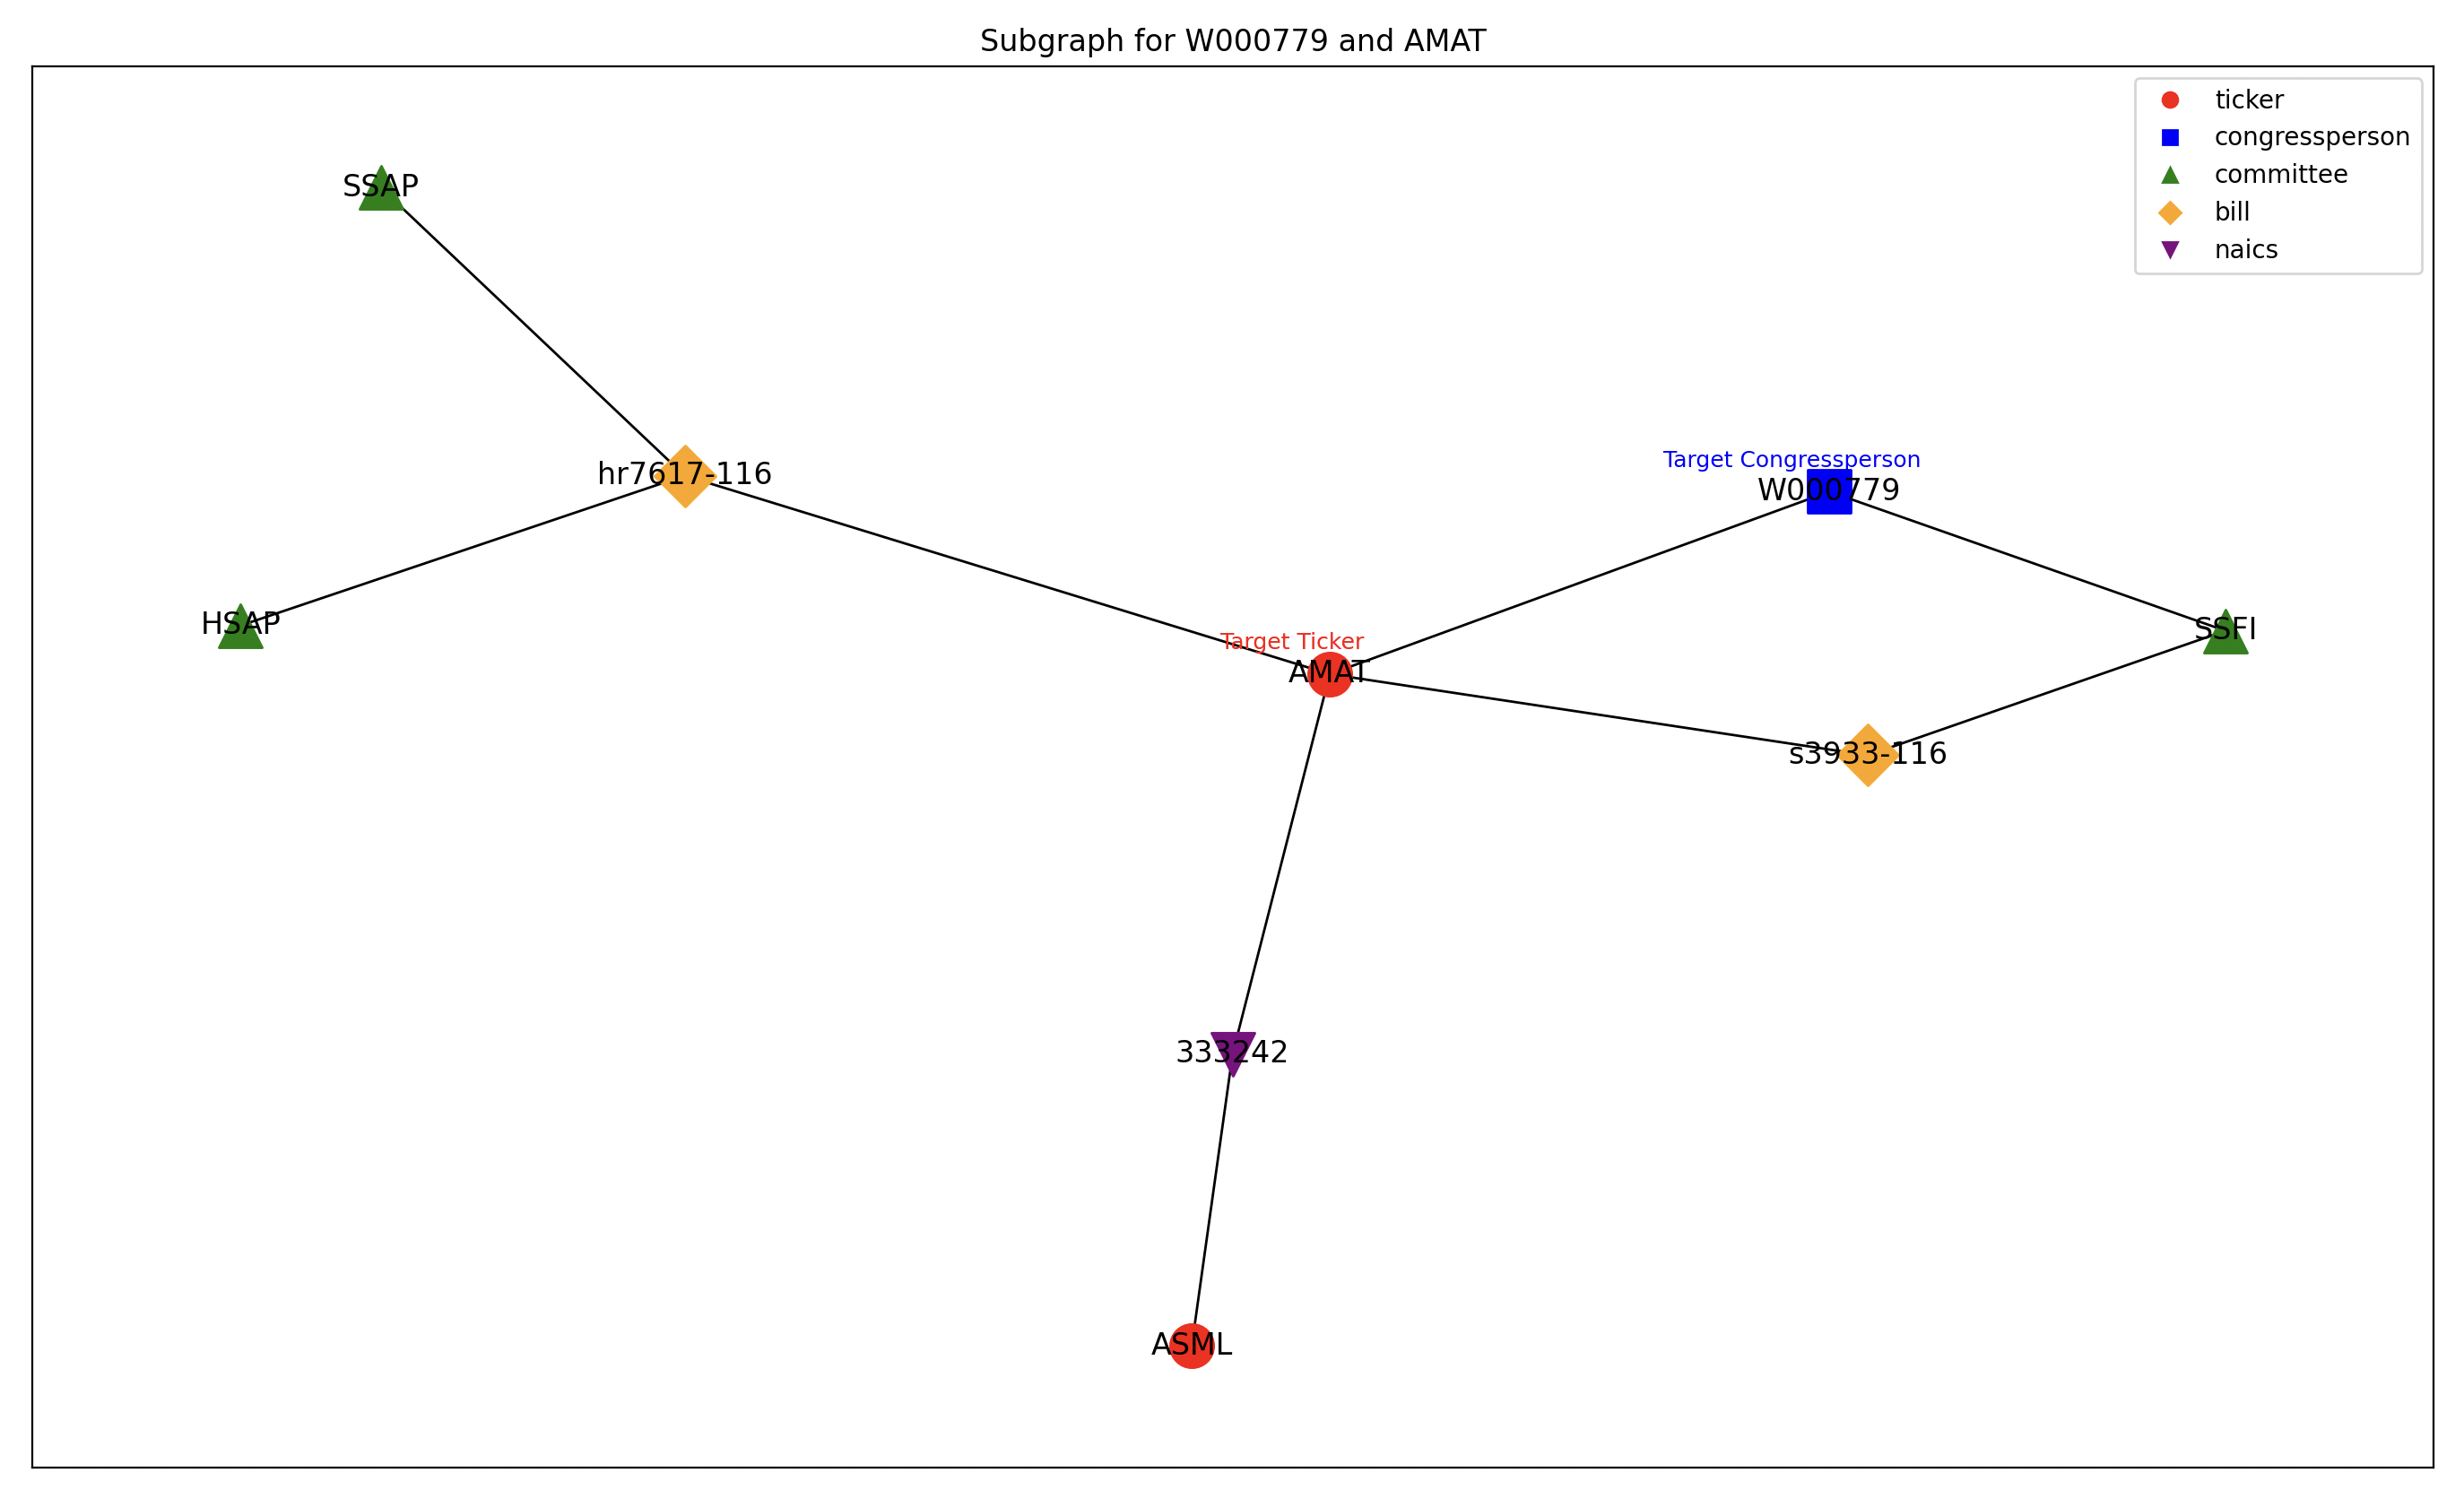
\includegraphics[width=1.1\textwidth, height=0.4\textheight]{imgs/gnnex-rw-amat.png}
  \caption{\textbf{GNNExplainer output for Senator Ron Wyden's transaction of AMAT's stock.} The figure shows the subgraph extracted from the entire graph using the node and edge masks trained by the GNNExplainer. The GNNExplainer identified S3933-116 (the CHIPS Act) and HR7617-116th among the bills that AMAT lobbied on, NAICS code 333242 (Semiconductor Machinery Manufacturing) among the NAICS code classifications of AMAT, and ASML, among the firms classified as 3333242 as the most influential factors for this transaction.}
  \label{fig:rw-amat}
  \end{figure}

Figure \ref{fig:rw-amat} focuses on Senator Ron Wyden's transaction of Applied Materials Inc. (AMAT)'s stock. To generate the subgraph from the entire graph, I applied the node and edge masks trained by the GNNExplainer. This process involved selecting the nodes and edges with the highest scores from the masks. For instance, among all 56 bills that AMAT lobbied on, I selected the two bills that had the highest scores in the edge mask. Similarly, among the two NAICS code classifications of AMAT, I selected the NAICS code 333242 (Semiconductor Machinery Manufacturing), which had the highest score in the edge mask.


The GNNExplainer successfully identified the most relevant bill for this transaction, S.3933-116, the CHIPS Act, which subsidizes the US semiconductor industry. Interestingly, the GNNExplainer also highlighted H.R.7617-116, a more general appropriations act, titled ``Defense, Commerce, Justice, Science, Energy and Water Development, Financial Services and General Government, Labor, Health and Human Services, Education, Transportation, Housing, and Urban Development Appropriations Act, 2021
''. While this bill may not be directly related to subsidization of the semiconductor industry, it is indicative of the broader legislative environment. It's worth noting that the National Defense Authorization Act (NDAA) for Fiscal Year 2021, which is often associated with appropriations for the semiconductor industry, was also part of the data. However, the GNNExplainer did not identify it as a highest score node for this particular transaction. This could be due to a variety of reasons, such as the complexity of the appropriations process or the indirect relationship between the NDAA and H.R.7617-116.

In addition to identifying relevant bills, the GNNExplainer also provided insights into the industry context of Senator Wyden's transaction of AMAT's stock. The NAICS code 333242, which corresponds to Semiconductor Machinery Manufacturing, includes four different companies: Applied Materials, ASML LLC (ASML), Azenta Inc (AZTA), and Tokyo Electron America Inc (TOELY). The GNNExplainer ranked ASML as the most relevant node for this transaction. This makes sense given the industry dynamics. While Azenta is a semiconductor company, it primarily focuses on bio-related semiconductor products, which may not be as directly relevant to AMAT's business. Tokyo Electron, on the other hand, is a much smaller firm compared to ASML or AMAT. Most importantly, ASML and AMAT are known to have a competitive relationship, with AMAT consistently striving to capture market share from ASML.
Therefore, the GNNExplainer's identification of ASML as the most relevant node for this transaction is consistent with the industry context.

As the chair of the Senate Finance Committee (SSFI), Senator Wyden has been a key player in initiatives related to the semiconductor industry. Despite the unexpected selection of H.R.7617-116 by the GNNExplainer, the overall results still highlight the relevance of Senator Wyden's legislative activities and industry context to his stock transactions.

\begin{figure}[h!]
  \centering
  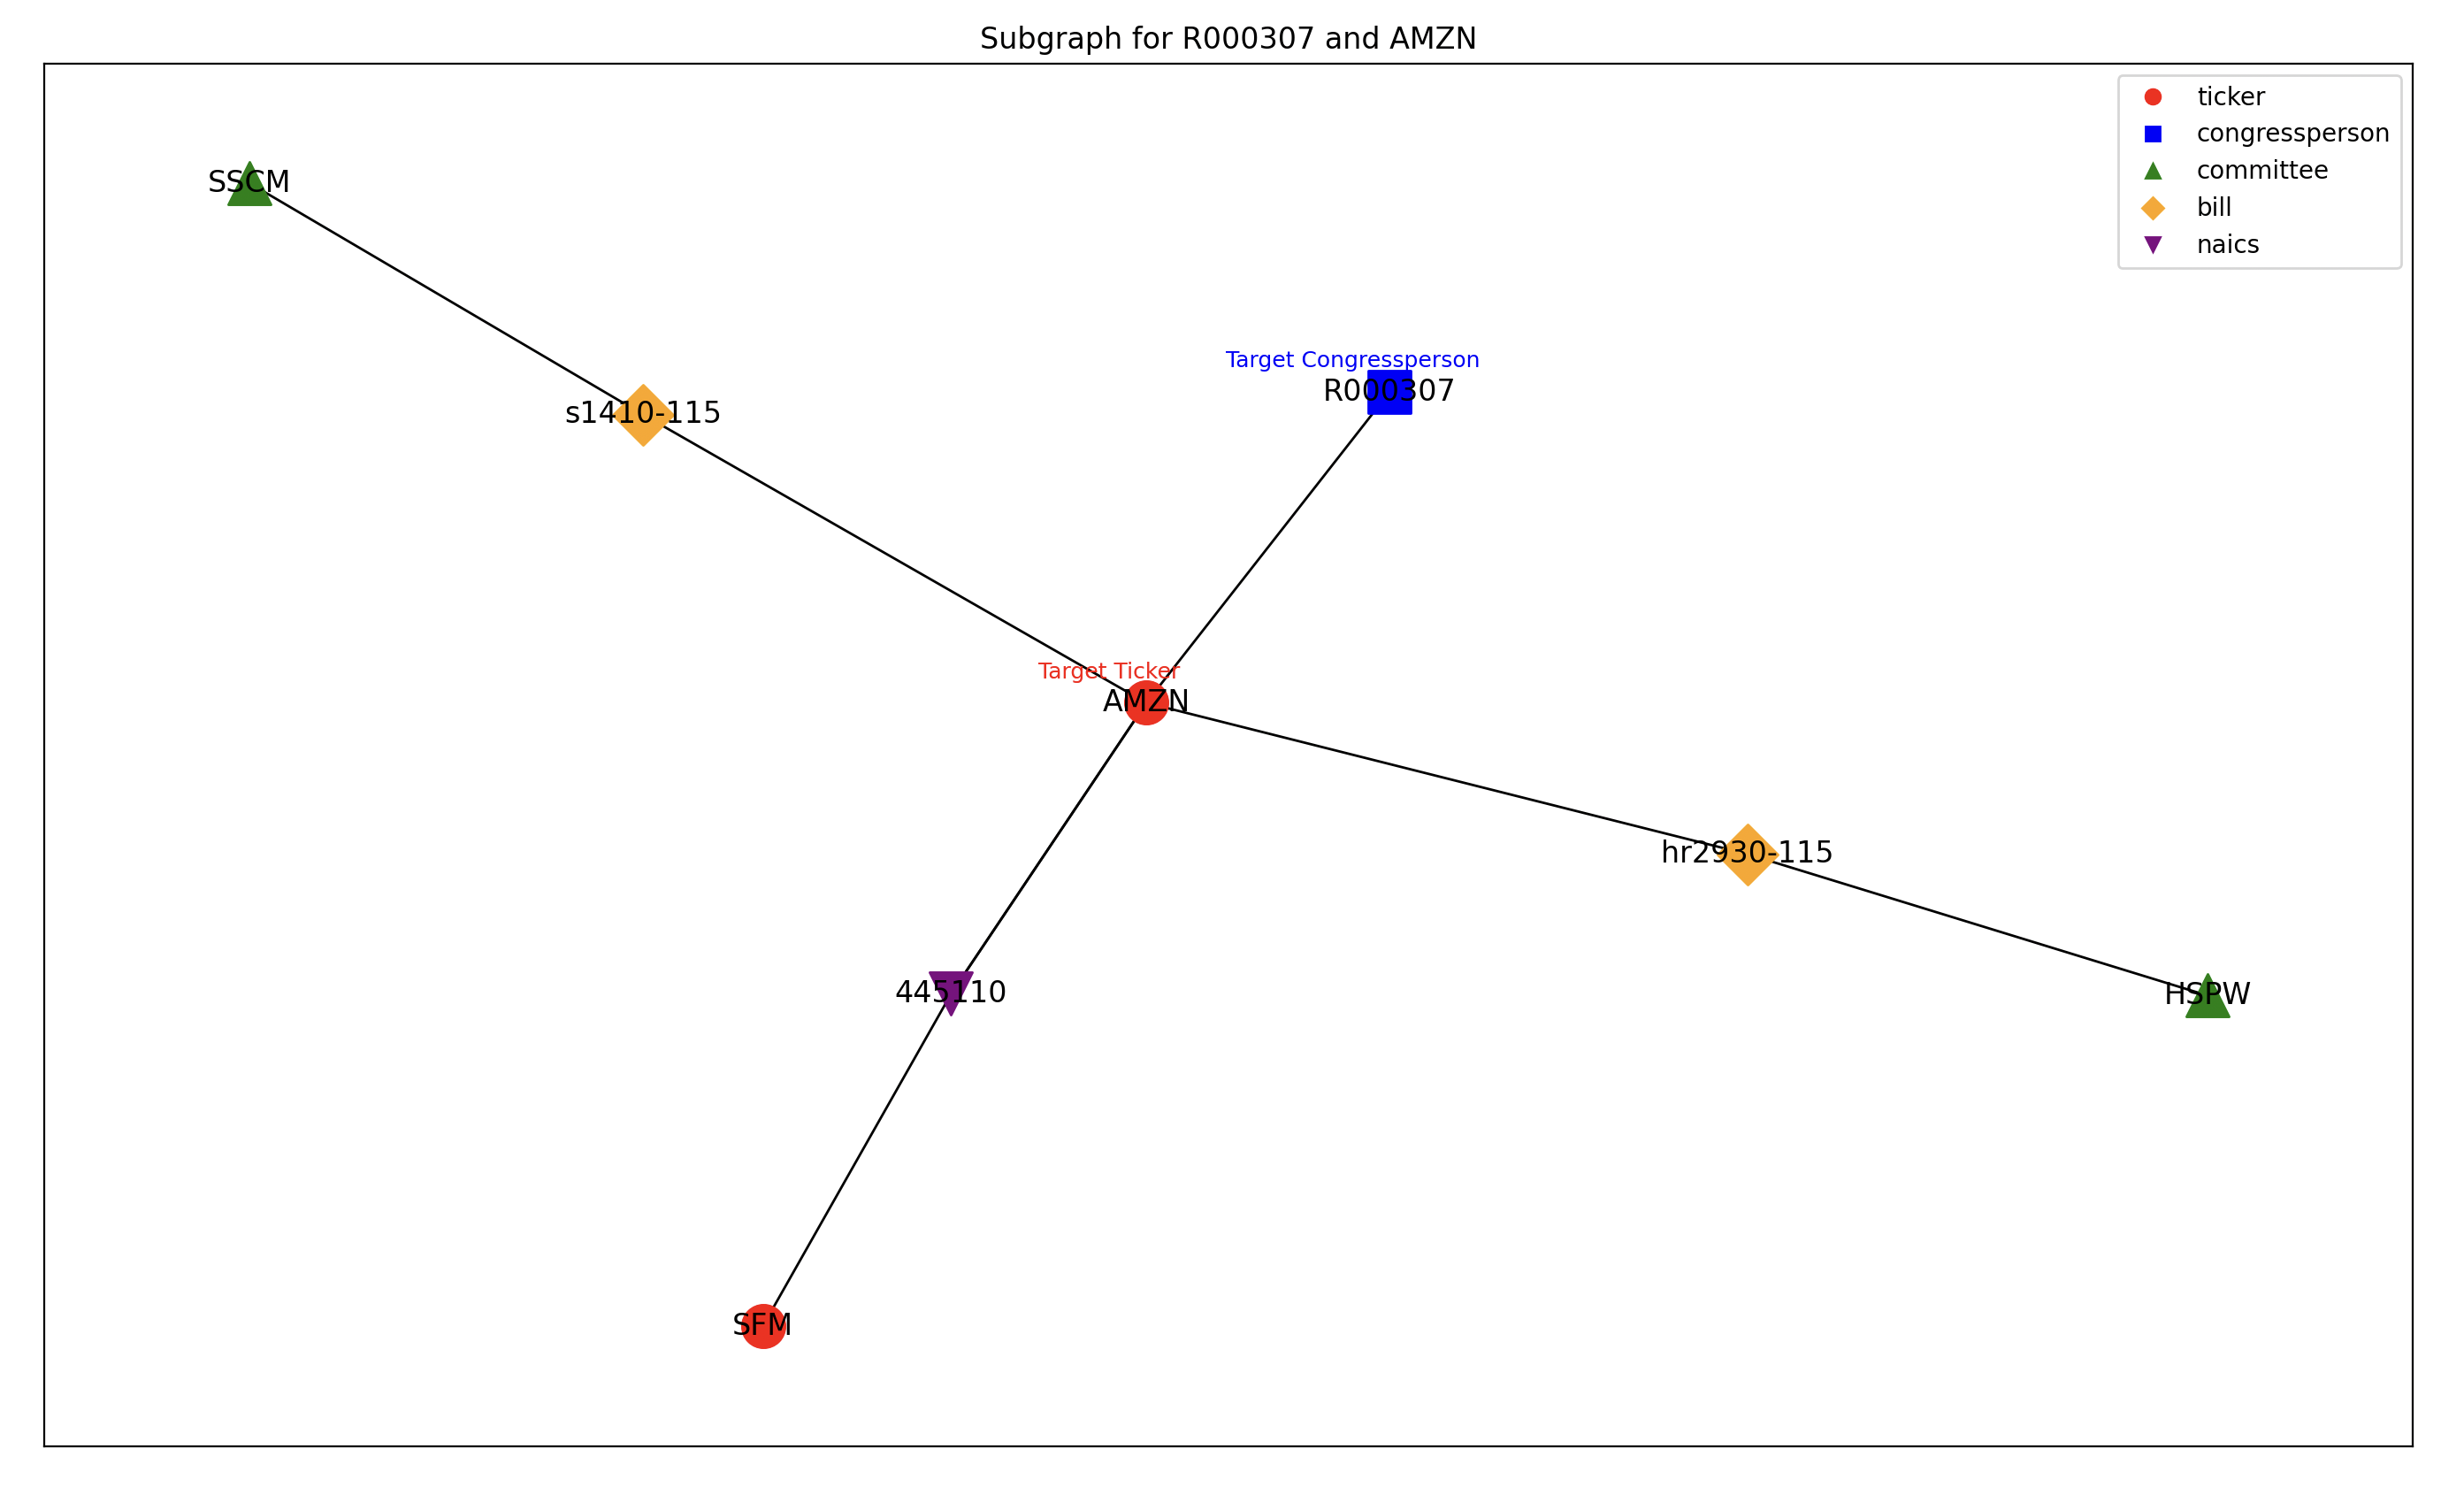
\includegraphics[width=1.1\textwidth, height=0.4\textheight]{imgs/gnnex-rob-pat.png}
  \caption{\textbf{GNNExplainer output for Senator Pat Roberts's transaction of Amazon's stock.} The figure shows the subgraph extracted from the entire graph using the node and edge masks trained by the GNNExplainer. The nodes and edges in the subgraph were selected based on their high scores in the masks, indicating their relevance to the model's prediction for this specific transaction. The GNNExplainer identified H.R.2930-115 (Drone Innovation Act of 2017) and S.1410 (Safe DRONE Act of 2017) among the bills that Amazon lobbied on as the most influential factors for this transaction. This is particularly interesting given Senator Roberts's known legislative activities related to drone technology.}
  \label{fig:pat-gnnex}
\end{figure}

Figure \ref{fig:pat-gnnex} presents another example, focusing on Senator Pat Roberts's transaction of Amazon (AMZN)'s stock. Among the 119 bills that Amazon lobbied on, the GNNExplainer identified H.R.2930-115 (Drone Innovation Act of 2017) and S.1410 (Safe DRONE Act of 2017) as the most relevant bills. This is particularly interesting because Senator Roberts co-sponsored the bill S.2730-116, which establishes a Drone Advisory Committee. Furthermore, 2017 was the year when Amazon started to publicize their plans for drone delivery\footnote{https://www.businessinsider.com/amazon-takes-critical-step-toward-drone-delivery-2017-5}. 
Therefore, we can interpret that Senator Roberts's transaction of Amazon's stock was likely influenced by his legislative activities related to drone technology.

Indeed, Figures 16 and 17 were not primarily intended to reinforce the main story that committee membership matters. Rather, they serve as an example of how the GNNExplainer can elucidate the decision-making process of the graph neural network for individual predictions. These figures showcase the ability of GNNExplainer to generate a plausible explanation for each specific prediction case, thereby providing a mechanism to interpret the predictions made by the neural network.
The ``black-box'' nature of neural networks is a common criticism \citep{bb4, bb5, bb6}, owing to their complex, high-dimensional, and non-linear decision-making process, which is often challenging to interpret and understand. This makes it difficult to trust their predictions, especially in sensitive contexts where understanding the reasoning behind predictions is essential. GNNExplainer addresses this criticism by providing a tool to interpret the predictions of the GNN, thereby making it more transparent and trustworthy.




% These examples demonstrate the ability of the GNNExplainer to highlight relevant legislative and industry context for specific stock transactions, even without explicit information about bill titles, text, or sponsorship relationships.
These examples demonstrate the ability of the GNNExplainer to highlight relevant legislative and industry context for specific stock transactions. It's noteworthy that the GNNExplainer was able to identify these relationships even without explicit information about bill titles, text, or sponsorship relationships. This suggests that the GNNExplainer is effectively capturing the underlying patterns in the data that are relevant for the prediction task.

% In conclusion, the GNNExplainer provides valuable insights into the specific nodes and edges that the model focuses on for its predictions. This allows us to pinpoint the specific legislative and industry factors that a congressperson is likely to consider when making stock transactions.

\section{Conclusion and Future Directions}
In this study, I delved into the dynamics of congressional stock investment, exploring what exactly influences these investment choices. My analysis aligned with the traditional financial literature's approach of excess return, which provided a direct estimation of possible excess return. This estimation addressed the range-censored limitation of the financial disclosure at the specific congress-ticker level, considering the life-cycle of transactions - from consecutive purchases to consecutive sales. This reconfirmed the findings of \cite{eg13}, which argued there was no widespread excess return among congressional investments. However, my findings indicate that such excess returns do exist at least abnormally and asymmetrically, more pronounced in the positive skewness compared to the negative returns. This suggests that some privileged information may drive such asymmetry in their excess return overall.

Secondly, I addressed a puzzle originating from the conclusions drawn by \cite{eg14}, who found no clear evidence that congresspersons disproportionately invested in stocks linked to their lobbying and committee assignments. This finding seemed somewhat counterintuitive and diverged from the extensive research on committee assignment and congresspersons' specialization in specific topics governed by committees. Stemming from this, I compiled a novel graph-structured dataset that more comprehensively captures congressional activities. This data utilizes a hetero-graph type, representing the interactions between different types of entities. Leveraging this dataset, I proposed a novel measure using cross-entropy, demonstrating that a congressperson's stock portfolio significantly resembles the stocks related to their assigned committees, compared to unassigned ones.

Thirdly, this study pioneers the application of a Large Language Model (LLM) Agent for automatic theorization in the realm of congressional stock trading analysis. This approach marks a contribution to the field, introducing a new method for generating theoretical hypotheses and potential explanations from complex high dimensional data sets.

Furthermore, I expanded on the work of \cite{eg14} by using the graph neural network to determine how possibly relevant factors, such as congressional activities captured in the graph data, predict congresspersons' stock transactions. The results showed that, contrary to \cite{eg14}, the committee assignment of congresspersons and lobbying activities of firms are the most important features predicting their stock selections. In addition, to address the black-box nature of predictions leveraging neural networks, I proposed using GNNExplainer \citep{gex}. This type of explainability method complements the evaluation metric to interpret case-by-case predictions and provides a more interpretable and semantically rich explanation of why a particular congressperson may choose certain stocks.

Adding onto these findings, it's worth examining the broader implications of our results. On a macro level, this research invites us to reassess our understanding of the motivations underpinning congressional service. The common perception is that congresspersons are primarily motivated by the goal of reelection, with their actions driven by a desire to serve their constituents and deliver policy outcomes that align with their promises and their party's platform.
However, our findings suggest that the picture may be more complex, with financial considerations also playing a significant role. The evidence that some congresspersons are able to achieve outsized returns on their stock investments points to the potential for personal financial gain to be a motivating factor in their decisions and actions. This raises profound questions about the alignment of incentives in our political system and the possibility of conflicts of interest.

On a micro level, the analysis reveals fascinating variations in the behavior of congresspersons when it comes to stock trading. While some closely mirror the stock transactions related to their committee assignments, others diverge considerably. This cautious behavior may be an attempt to avoid the appearance or reality of insider trading, a legal and ethical boundary that all congresspersons must navigate.
Unraveling the sources of these behavioral differences presents an intriguing avenue for further research. Are these variations simply a reflection of individual personalities, strategic thinking, and risk tolerance? Or are they indicative of deeper systemic factors within our political and financial systems that are yet to be fully understood?

Could the differences in trading patterns, for instance, be linked to the disparities in the level of scrutiny that different congresspersons face, their connections within the industry, or the financial literacy they possess? Do congresspersons with certain committee assignments have more access to non-public market-moving information? Uncovering these underpinnings would offer a more nuanced understanding of the complex interplay between politics and finance and could inform policy decisions to improve transparency and fairness in our political system.

% In conclusion, this research contributes to existing literature in three significant ways. First, it confirms the non-widespread excess return among congresspersons but suggests that they systematically acquire positive excess return compared to their losses. Secondly, this research highlights the importance of committee assignments in explaining congressional stock trading, resolving the potential puzzle instigated by Eggers and Hainmueller (2014). Thirdly, it illustrates the utility of graph-structured data and graph neural networks in understanding which features carry the most critical information to explain congressional stock trading overall.


\bibliography{biblo.bib}

\appendix
\section{Data Merging and Entity Disambiguation}\label{app:disambiguation}

One of the key challenges to make this graph-structured data is the effective disambiguation of entities, as the data is collected from multiple sources, including LobbyView, Senate/House Financial Disclosures, and naics.com. In this graph-structured dataset, entities such as Congresspersons and firms may appear under different names or expressions. For example, ``Ron Wyden'' may also be referred to as ``Ron L. Wyden'', and ``Apple'' may appear as ``Apple Inc.''. To accurately disambiguate these differing text representations of entities, it is essential to establish a unique identifier for each entity, regardless of the variations in their names.

Theoretically, matching entities based on text similarity between two datasets with $n$ and $m$ rows has a computational complexity of 
$O(n m)$ \citep{onm}. 
Therefore, as the datasets grow larger, this complexity becomes prohibitively expensive. For instance, matching 70,000 firm names from LobbyView to 4,000 firm names appearing in the ticker table would require 280,000,000 times of computations for text similarity. To address this challenge, I developed a novel approach that leverages URLs as unique identifiers for entities.

The approach involves acquiring the corresponding URL for each entity through Google searches, such as \url{https://en.wikipedia.org/wiki/Ron_Wyden} for Ron Wyden and \url{https://www.apple.com/} for Apple, Inc. A key advantage of using URLs as unique identifiers is that they facilitate effective entity disambiguation. For example, if two different expressions, ``Ron Wyden'' and ``Ron L. Wyden'' are both assigned the same URL \url{https://en.wikipedia.org/wiki/Ron_Wyden}, we can confidently recognize that these two expressions refer to the same entity. This approach allows us to accurately consolidate information about entities that may be represented in various ways across different data sources. Additionally, this method reduces the computational complexity to 
$O(n+m)$, as only one query is required for each row of data. To further scale up this process, I parallelized the URL acquisition process by batching queries and distributing them across multiple servers available through commercial cloud services like AWS.

\section{Effective Parsing Technique for Financial Disclosures}\label{app:par}

Financial Disclosures from the House are provided as encrypted PDF files. While text can be extracted from these files, the encryption results in irregular patterns, particularly in the tables that contain information about Congresspersons' stock buying and selling activities. These irregular patterns make it challenging to parse the data using manually coded patterns, as the deviations are difficult to anticipate and account for. To address this challenge, I utilized OpenAI's APIs, specifically the GPT-3.5 Turbo language model, to parse the PDFs into a CSV format that includes information such as when and who bought or sold which ticker, and how much.

The process involves querying the Large Language Model (LLM) with the extracted text from the PDFs and instructing the model to convert the irregularly formatted tables into structured CSV data which includes columns such as the date of the transaction, the name of the Congressperson, the ticker symbol of the stock, the type of transaction (buy or sell), and the amount of the transaction.

By leveraging the capabilities of the GPT-3.5 Turbo language model, I was able to effectively parse information contained in PDF files that would normally require manual human labor. This approach significantly streamlines the data extraction process and ensures the accuracy and consistency of the parsed data.


In summary, this innovative approach to entity disambiguation through URL acquisition and parallelization enables efficient data merging from diverse sources, ensuring the accuracy and scalability of the analysis.

\section{Appendix: Task \& Reflection Prompt and Detailed Log from LLM Agent Performing Prediction and Reflection} \label{app:log}

\subsection*{Task Prompt for the Agent to Perform `Make\_Prediction'}\label{app:log:task_prompt}
\begin{Verbatim}[breaklines=true, frame=single]
You are granted access to a graph database that encompasses interactions and activities related to the U.S. Congress, its Legislators, and publicly traded companies. 
Your mission is to deduce the probability of a financial transaction between a designated U.S. Legislator, {Legis}, and a specific publicly traded company or ETF, {Company}, whose ticker is {Ticker} and name is {Company}.

Available Nodes:
- Legislator: Represents members of the U.S. Congress. Essential attributes include their 'name' and an identifier called 'bioguide'.
- Ticker: Symbolizes publicly traded companies or ETF on stock exchanges. Each company or ETF is uniquely identified by its 'ticker' symbol, a shorthand used on stock trading platforms, and it has additional property 'name', the official corporate designation or name of the ETF.
- Committee: Stands for the specialized committees within the U.S. Congress, each of which focuses on specific domains like finance, defense, health, or education. Crucial properties include 'name' and 'id'.
- NAICS: Corresponds to the North American Industry Classification System, which categorizes businesses and industries. Pertinent attributes are 'ticker' and 'desc', which describe the sector or industry where 
a publicly traded company belongs.
- Bill: Denotes legislative bills processed within the U.S. Congress. Essential attributes include 'summary', 'id', 'official_title', and 'short_title'.

Available Relationships:
- BUY_SELL: Indicates a financial transaction or stock trading activity between a U.S. Legislator and a publicly traded company, with date specifics. (Legislator -> BUY_SELL -> Ticker)
- COMMITTEE_ASSIGNMENT: Relays the assignment of a U.S. Legislator to a specific Committee within Congress for a set tenure. (Legislator -> COMMITTEE_ASSIGNMENT -> Committee)
- LOBBY_ON: Chronicles the endeavors where a publicly traded company, via its Ticker, lobbied a particular Bill. (Ticker -> LOBBY_ON -> Bill). However, ETF does not lobby on a bill like QQQ or SPY.
- BELONGS_TO: Designates the industry or sector, as per the NAICS system, where a publicly traded company operates. (Ticker -> BELONGS_TO -> NAICS)
- ASSIGNED_TO: Signals the allocation of a Bill to a distinct Committee within Congress. (Bill -> Assigned_to -> Committee)

[TASK]
Using the information, scrutinize the nodes and relationships to estimate the likelihood of a "BUY_SELL" link between {Legis} and {Ticker}. You should give your guess (prediction) about a EXIST or NOT-EXIST of the transaction between {Legis} and {Ticker} as a final answer. 

[Note]
1. For the purposes of this task, any existing direct "BUY_SELL" relationships between {Legis} and {Ticker} have been intentionally deleted from graph database. Your goal is to infer the likelihood of such a relationship based on indirect data points.
Therefore, make sure that 
    - 1. You don't need to check whether there exist a direct "BUY_SELL" relationship between {Legis} and {Ticker} because it's already and intentionally deleted if exists.
    - 2. You should "guess" a EXIST or NOT-EXIST of the transaction between {Legis} and {Ticker} as a final answer.

2. When you fetch the bill node, do not fetch the `summary` attribute of the node because it's too long and this will deplete your Token limits to conduct the task successfully. Instead, you should fetch the `official_title` attribute of the node to understand the bill's content.

[Harnessing the Memory Vector Database]
You have a Memory Vector Database that encapsulates key strategies derived from your history of analyzing legislator-company stock transactions. This tool operates on a principle of condition-action pairs:

    Condition: A specific scenario or set of circumstances from past tasks.
    Action: The strategic response that was effective in that scenario.

When faced with a new task, the database can be leveraged as follows:

Describe the Condition: Input a description of the current task's conditions into the database. Then the database uses vector similarity to find past conditions that closely match your description.
It then presents you with a list of condition-action pairs that were effective in similar past scenarios. This process helps you to quickly identify the most relevant strategies for the current task, drawing on successful experiences to inform your decision-making.

The following is a list of condition-action pairs that you may be able to find in the database:
    [Example 1]
        Condition: Scenarios where a legislator has multiple overlapping NAICS codes with the tickers they've engaged in transactions with.
        Action: In such scenarios, confidently assert the existence of a relationship.

    [Example 2]
        Condition: Situations where there are no overlapping NAICS codes between a ticker and the legislator's transactions.
        Action: In these instances, scrutinize any bill titles lobbied by the ticker that are pertinent to the committees the legislator belongs to.

In addition, make sure you start your chain-of-action by using this "Memory" tool by describing your task so that you can more faster and more accurately solve the task.  
\end{Verbatim}


\subsection*{Detailed Log of the Agent's Make\_Prediction Process: Ron Wyden - Applied Materials (AMAT)}\label{app:log:make_prediction}

\begin{Verbatim}[breaklines=true, frame=single]
> Entering new AgentExecutor chain...
To begin with, I need to assess the indirect data points that could suggest a financial transaction between Ron Wyden and AMAT. Since direct "BUY_SELL" relationships have been intentionally deleted, I should look for overlapping interests, such as committee assignments, bills lobbied by AMAT, and NAICS codes that might indicate a connection between the legislator and the company.  
  
Action: MemoryDB Query
Action Input: I am trying to predict whether a "BUY_SELL" relationship exists between Ron Wyden and AMAT based on indirect data points such as committee assignments, bills lobbied by AMAT, and overlapping NAICS codes, despite the direct relationship being intentionally deleted from the database.

Observation: [{'condition': "Predicting a 'BUY_SELL' relationship between a legislator and an ETF based on indirect data points, where the ETF targets multiple companies in the same industry or theme.", 'action': "Consider the legislator's committee assignments, the bills lobbied by the ETF, and the sectors or industries where the ETF operates. Check for any overlap between the committees that the legislator is assigned to and the bills that the ETF has lobbied on. Also check if the legislator has had any financial transactions with companies in the same industry as the ETF."}, {'condition': "When there is a lack of data or relationships to infer the likelihood of a 'BUY_SELL' link between a legislator and a company.", 'action': "In these instances, consider other factors such as the legislator's overall trading activity, the company's overall lobbying activity, and the general trends in the legislator's transactions and the company's lobbying activities. Use these factors to make an educated guess about the likelihood of a 'BUY_SELL' link."}]
  
Thought:Based on the observations from the Memory tool, I should consider Ron Wyden's committee assignments, the bills lobbied by AMAT, and the NAICS codes related to AMAT. I should check for any overlap between the committees that Ron Wyden is assigned to and the bills that AMAT has lobbied on. Additionally, I should consider if Ron Wyden has had any financial transactions with companies in the same industry as AMAT. Since direct "BUY_SELL" relationships are intentionally deleted, I need to use these indirect data points to make an educated guess about the likelihood of a "BUY_SELL" relationship.

Action: GraphDB Query
Action Input: 
MATCH (l:Legislator {name: 'Ron Wyden'})-[:COMMITTEE_ASSIGNMENT]->(c:Committee)<-[:ASSIGNED_TO]-(b:Bill)<-[:LOBBY_ON]-(t:Ticker {ticker: 'AMAT'})
RETURN DISTINCT c.name, b.official_title

Observation: [[{'c.name': 'Senate Committee on the Judiciary', 'b.official_title': 'To amend the Immigration and Nationality Act to eliminate the per-country numerical limitation for employment-based immigrants, to increase the per-country numerical limitation for family-sponsored immigrants, and for other purposes.'}
, {'c.name': 'Senate Committee on Finance', 'b.official_title': 'A bill to amend the Internal Revenue Code of 1986 to establish the semiconductor manufacturing investment credit.'}, 
{'c.name': 'House Committee on Energy and Commerce', 'b.official_title': 'To restore American leadership in semiconductor manufacturing by increasing Federal incentives in order to enable advanced research and development, secure the supply chain, and ensure long-term national security and economic competitiveness.'}, 
{'c.name': 'Senate Committee on Finance', 'b.official_title': 'A bill to restore American leadership in semiconductor manufacturing by increasing Federal incentives in order to enable advanced research and development, secure the supply chain, and ensure long-term national security and economic competitiveness.'}, 
{'c.name': 'House Committee on Energy and Commerce', 'b.official_title': 'To modernize and strengthen the Committee on Foreign Investment in the United States to more effectively guard against the risk to the national security of the United States posed by certain types of foreign investment, and for other purposes.'}, 
{'c.name': 'Senate Committee on Finance', 'b.official_title': 'A bill to amend the Internal Revenue Code of 1986 to enhance tax benefits for research activities.'}, {'c.name': 'Senate Committee on the Judiciary', 'b.official_title': 'A bill to amend the Immigration and Nationality Act to eliminate the per-country numerical limitation for employment-based immigrants, to increase the per-country numerical limitation for family-sponsored immigrants, and for other purposes.'}, 
{'c.name': 'House Committee on Energy and Commerce', 'b.official_title': 'To establish a new Directorate for Technology and Innovation in the National Science Foundation, to establish a regional technology hub program, to require a strategy and report on economic security, science, research, innovation, manufacturing, and job creation, to establish a critical supply chain resiliency program, and for other purposes.'}, 
{'c.name': 'Senate Committee on Commerce, Science, and Transportation', 'b.official_title': 'A bill to establish a new Directorate for Technology and Innovation in the National Science Foundation, to establish a regional technology hub program, to require a strategy and report on economic security, science, research, innovation, manufacturing, and job creation, to establish a critical supply chain resiliency program, and for other purposes.'}, 
{'c.name': 'Senate Committee on the Judiciary', 'b.official_title': 'A bill to amend the Immigration and Nationality Act to authorize additional visas for well-educated aliens to live and work in the United States, and for other purposes.'}, 
{'c.name': 'House Committee on Energy and Commerce', 'b.official_title': 'To provide for a coordinated Federal research initiative to ensure continued United States leadership in engineering biology.'}]]

Thought:The query results show that there are bills related to semiconductor manufacturing and technology innovation that have been lobbied on by AMAT and are assigned to committees that Ron Wyden is a member of, particularly the Senate Committee on Finance. This suggests that there is an overlap in the interests of Ron Wyden and AMAT, which could be an indicator of a potential "BUY_SELL" relationship. 
Next, I should check if Ron Wyden has had any financial transactions with companies in the same industry as AMAT to further support the likelihood of a "BUY_SELL" relationship.

Action: GraphDB Query
Action Input: 
MATCH (l:Legislator {name: 'Ron Wyden'})-[:BUY_SELL]->(t:Ticker)-[:BELONGS_TO]->(n:NAICS)
WHERE EXISTS((:Ticker {ticker: 'AMAT'})-[:BELONGS_TO]->(n))
RETURN DISTINCT t.ticker, n.desc
Parsing Cypher queries...
Input text: MATCH (l:Legislator {name: 'Ron Wyden'})-[:BUY_SELL]->(t:Ticker)-[:BELONGS_TO]->(n:NAICS)
WHERE EXISTS((:Ticker {ticker: 'AMAT'})-[:BELONGS_TO]->(n))
RETURN DISTINCT t.ticker, n.desc


Observation: [[{'t.ticker': 'AVGO', 'n.desc': 'Semiconductor and Related Device Manufacturing'}, {'t.ticker': 'INTC', 'n.desc': 'Semiconductor and Related Device Manufacturing'}, {'t.ticker': 'NVDA', 'n.desc': 'Semiconductor and Related Device Manufacturing'}]]

Thought:The results indicate that Ron Wyden has engaged in financial transactions with other companies in the semiconductor and related device manufacturing industry, which is the same industry as AMAT. This further supports the likelihood of a "BUY_SELL" relationship between Ron Wyden and AMAT, as there is a pattern of interest in this sector.
Given the overlap in committee interests and the legislator's previous financial transactions within the same industry as AMAT, I can make an educated guess about the existence of a "BUY_SELL" relationship.

Final Answer: Based on the indirect data points such as committee assignments related to technology and semiconductor manufacturing, bills lobbied by AMAT that are assigned to these committees, and Ron Wyden's financial transactions with other companies in the same industry, it is likely that a "BUY_SELL" relationship between Ron Wyden and AMAT exists (EXISTS).

> Finished chain.
\end{Verbatim}

\subsection*{Reflection Prompt for the Agent to Perform `Generate\_Reflection'}\label{app:log:reflect_prompt}
\begin{Verbatim}[breaklines=true, frame=single]
  Previously, I presented you with a link prediction task:

  [Previous TASK]-----------------
  {Task Prompt}
  -------------------------------

  Your response was:

  [LOG]---------------------------
  {Log from Make_Prediction}
  --------------------------------

  % Either one of the below two lines based on eval:
  Your response was ACCURATE, as there is indeed a "BUY-SELL" relationship between "{Legis}" and "{Ticker}".

  Your response was INACCURATE, as there exists a "BUY-SELL" relationship between "{Legis}" and "{Ticker}".  


  Moving on, your next objective involves self-reflection:

  [TASK]
  Building upon your failure with the previous task, take a moment to consider the key factors that contributed to your failure. Then reflect on how and when certain strategies can be applied in future scenarios to avoid such failure. 
  Now that you know the answer of the task, you can try multiple possible queries using the tool GraphDB Query to see which features of the data could have helped you to solve the task.

  Then, structure your self-assessment in two parts:

  Condition: Identify specific conditions under which the strategy you came up with reflection employed.
  Action: Outline the steps of the strategy to be employed under these conditions.

  This analysis will serve as a guide for tackling similar tasks in the future, where "similarity" is determined by the conditions you delineate. You will be provided with a new task later on, along with a tool to detect conditions akin to those you've described by assessing vector similarity, enabling you to retrieve and apply the successful action from your previous experience.

  For example:

      [Example 1]
          Condition: Scenarios where a legislator has multiple overlapping NAICS codes with the tickers they've engaged in transactions with.
          Action: In such scenarios, confidently assert the existence of a relationship.

      [Example 2]
          Condition: Situations where there are no overlapping NAICS codes between a ticker and the legislator's transactions.
          Action: In these instances, scrutinize any bill titles lobbied by the ticker that are pertinent to the committees the legislator belongs to.

  However, as you reflect on the task you've just completed, distill a novel condition-action pair that captures a new understanding or strategy not previously recorded in your memory. This pair should be informed by unique aspects or outcomes of the current task. If no new insights have emerged or if the task's conditions do not warrant a fresh approach distinct from existing entries, please return an empty list.


  [Output Format]
  We want your answer to be jsonl format with the list of your pair of "Condition" and "Action" as follows:

  [{{
  "condition": "Instances where a legislator has several overlapping NAICS codes among the tickers they've transacted with.",
  "action": "In such a data landscape, confidently indicate 'EXIST'."
  }}, ... ] # store multiple pairs of "Condition" and "Action" in a list if you have multiple pairs of "Condition" and "Action" to store in your memory.
\end{Verbatim}


\subsection*{Detailed Log of the Agent's `Generate\_Reflection' Process: Ron Wyden-Applied Materials (AMAT)}\label{app:log:reflect}

\begin{Verbatim}[breaklines=true, frame=single]
  > Entering new AgentExecutor chain...
  To complete the self-assessment, I need to identify the conditions under which the strategy I previously employed can be effectively utilized and outline the steps of the strategy to be employed under these conditions.
  
Action: Memory
Action Input: I need to reflect on the key factors that contributed to the successful prediction of a "BUY_SELL" relationship between Ron Wyden and AMAT, and how to apply similar strategies in future scenarios with similar conditions.
Observation: [{'condition': "Predicting a 'BUY_SELL' relationship between a legislator and an ETF based on indirect data points, where the ETF targets multiple companies in the same industry or theme.", 'action': "Consider the legislator's committee assignments, the bills lobbied by the ETF, and the sectors or industries where the ETF operates. Check for any overlap between the committees that the legislator is assigned to and the bills that the ETF has lobbied on. Also check if the legislator has had any financial transactions with companies in the same industry as the ETF."}, {'condition': "When there is a lack of data or relationships to infer the likelihood of a 'BUY_SELL' link between a legislator and a company.", 'action': "In these instances, consider other factors such as the legislator's overall trading activity, the company's overall lobbying activity, and the general trends in the legislator's transactions and the company's lobbying activities. Use these factors to make an educated guess about the likelihood of a 'BUY_SELL' link."}, {'condition': "When predicting a 'BUY_SELL' relationship between a legislator and a ticker, and there are no indirect relationships between them in the graph database.", 'action': "In these instances, consider the possibility of a direct 'BUY_SELL' relationship between the legislator and the ticker. Use a query to check for such a direct relationship. If there is a direct 'BUY_SELL' relationship, confidently assert the existence of a relationship."}]

Thought:I now have a list of condition-action pairs that were effective in similar past scenarios. I can use these to create a self-assessment of the strategy I employed in the current task.

Final Answer:
```jsonl
[
    {
        "condition": "When a legislator's committee assignments overlap with bills lobbied by a company.",
        "action": "Use a Cypher query to identify any overlap between the committees a legislator is assigned to and the bills a company has lobbied on. 
        If overlap exists, this suggests a potential 'BUY_SELL' relationship. Cypher query example: MATCH (l:Legislator)-[:COMMITTEE_ASSIGNMENT]->(c:Committee)<-[:ASSIGNED_TO]-(b:Bill)
        <-[:LOBBY_ON]-(t:Ticker) RETURN DISTINCT c.name, b.official_title"
    },
    {
        "condition": "When a legislator has engaged in financial transactions with companies in the same industry as another company.",
        "action": "Use a Cypher query to check if a legislator has had financial transactions with companies in the same NAICS industry as the company in question. If transactions exist, this indicates a higher likelihood of a 'BUY_SELL' relationship. Cypher query example: MATCH (l:Legislator)-[:BUY_SELL]->(t:Ticker)-[:BELONGS_TO]->(n:NAICS) WHERE EXISTS((:Ticker)-[:BELONGS_TO]->(n)) RETURN DISTINCT t.ticker, n.desc"
    }
]
```
> Finished chain.

\end{Verbatim}

% \section*{Detailed Memory Pairs of the LLM Agent}

% \subsection*{Memory Pair 1}
% \textbf{Condition:} When there is no direct 'BUY\_SELL' relationship data available, but there is indirect evidence of a connection between a legislator's committee assignments and a ticker's lobbying activities on related bills.

% \textbf{Action:} Use indirect evidence such as committee assignments and bill lobbying to infer the likelihood of a 'BUY\_SELL' relationship.

% \textbf{Cypher Query:} 
% \begin{verbatim}
% MATCH (l:Legislator {bioguide: '<bioguide>'})-[:COMMITTEE_ASSIGNMENT]->(c:Committee)
% <-[:ASSIGNED_TO]-(b:Bill)<-[:LOBBY_ON]-(t:Ticker {ticker: '<Ticker>'}) 
% RETURN l.name, c.name, b.official_title, t.ticker
% \end{verbatim}

% % Repeat the above format for each memory pair, changing the content accordingly.

% \subsection*{Memory Pair 2}
% \textbf{Condition:} When a legislator has a history of transactions with companies across diverse sectors, and the ETF in question also represents a broad range of sectors.

% \textbf{Action:} Predict the existence of a 'BUY\_SELL' relationship between the legislator and the ETF, considering the legislator's broad investment interests and the ETF's diverse sector coverage.

% \textbf{Cypher Query:} None specific; general prediction based on behavioral patterns.


% \subsection*{Memory Pair 27}
% \textbf{Condition:} When there is an overlap in NAICS sectors between the companies a legislator has transacted with and the industry of a ticker, and direct 'BUY\_SELL' relationships are intentionally deleted from the database.

% \textbf{Action:} Predict 'EXIST' for a 'BUY\_SELL' relationship between the legislator and the ticker, as the overlap in NAICS sectors suggests a potential alignment of interests that could lead to financial transactions.

% \textbf{Cypher Query:} 

\end{document}


\end{document}